\documentclass{tstextbook}

% \documentclass[11pt]{report}
% \documentclass[11]{book}
% \usepackage[dutch]{babel}
% \usepackage{a4wide}
\usepackage{epsfig}
\usepackage{wrapfig}
\usepackage{subfigure}
\usepackage{graphics}
\usepackage{subfigure}
\usepackage{fancyvrb}
\usepackage{algorithm}
\usepackage{algpseudocode}
\usepackage{units}
% \usepackage{amsthm}
% \renewcommand{\thepage}{\hspace*{-3cm}\arabic{page}}

\usepackage{paralist}
\usepackage{hyperref}

\setlength{\textwidth}{15cm}
\setlength{\oddsidemargin}{0.5cm}
\setlength{\evensidemargin}{0.5cm}
\setlength{\textheight}{20cm}

% \usepackage{titlesec}

\usepackage{amssymb}

\usepackage{shadow}
\usepackage{xcolor}
\usepackage{soul}
% \newcommand{\grijs}[1]{\fcolorbox{gray}{gray}{#1}}
\definecolor{shadecolor}{RGB}{230,230,230}
\newcommand{\grijs}[1]{\par\colorbox{shadecolor}
  {\parbox{\dimexpr\textwidth-2\fboxsep\relax}{#1}}}

\newcommand{\bart}[1]{\marginpar{\color{red} Bart}\textbf{\color{blue}[#1]}}
\newcommand{\marton}[1]{\marginpar{\color{red} Marton}\textbf{\color{red}{#1}}}
\newcommand{\martonst}[2]{\marginpar{\color{red} Marton}\textbf{\color{red}{\st{#1}$~\mapsto~${#2}}}}

%\renewcommand\qedsymbol{$\blacksquare$}

\newcommand{\N}{\mathbb{N}}
\newcommand{\Z}{\mathbb{Z}}
\newcommand{\Q}{\mathbb{Q}}
\newcommand{\R}{\mathbb{R}}
\newcommand{\C}{\mathbb{C}}



%fancy heading
% \usepackage{fancyhdr}
% \pagestyle{fancy}


%  Een paar definities
% \renewcommand{\thesection}{\arabic{section}}
\newcommand{\ds}{\displaystyle}
\newcommand{\bin}[2]{{{\ds #1} \choose {\ds #2}}}
\newcommand{\prend}{\hfill \rule{2.3mm}{2.3mm} \hspace*{3mm} $ $}
\newcommand{\rpijl}{$\rightarrow~$}
\newcommand{\eps}{$\epsilon~$}
\newcommand{\project}[1]{}

\newcommand{\myref}[1]{~\ref{#1} on page~\pageref{#1}}

\newtheorem{stelling}{Theorem}[section]
\newtheorem{definitie}[stelling]{Definition}
\newtheorem{informeledefinitie}[stelling]{Informal definition}
%\newtheorem{lemma}[stelling]{Lemma}
\newtheorem{algo}[stelling]{Algorithm}
\newtheorem{eig}[stelling]{Property}
\newtheorem{gevolg}[stelling]{Consequence}
\newtheorem{vb}[stelling]{Example}




\lhead[\fancyplain{}{\rm\thepage}]{\fancyplain{}{\rightmark}}
\chead[]{}
\rhead[\fancyplain{}{\leftmark}]{\fancyplain{}{\rm\thepage}}
\lfoot[]{}
\cfoot[]{\fancyplain{\rm\thepage}{}}
\rfoot[]{}

% nu degene zonder nummer
% \newtheorem{vb}{Voorbeeld}
% \renewcommand{\thevb}{}

\setlength{\parindent}{0cm}

\renewcommand{\P}{{\bf P} }
\newcommand{\NP}{{\bf NP} }
\newcommand{\LL}{{\bf L} }
\newcommand{\NL}{{\bf NL} }
\newcommand{\NPC}{{\bf NPC} }
\newcommand{\PSPACE}{{\bf PSPACE} }
\newcommand{\NPSPACE}{{\bf NPSPACE} }
\newcommand{\EXP}{{\bf EXP} }
\newcommand{\NEXP}{{\bf NEXP} }


\begin{document}

\tsbook{Fundamentals for Computer Science}
       {Bart Demoen, Tom Schrijvers}
       {Tobias van Schneider}
       {2019}
       {xxxxx}{xxx--xx--xxxx--xx--x}{1.0}
       {}
       {Leuven}

% %% TITELBLAD
% \renewcommand{\thepage}{}
% % \pagestyle{plain}
%
%
%
% \begin{center}
% \shabox{\Huge \bf Fundamentals for Computer Science}
% ~~\\
% ~~\\
% ~~\\
% ~~\\
% 
\includegraphics[%
%   width=0.1\linewidth,
%   keepaspectratio]{afbeeldingen/sedes}
% ~~\\
% ~~\\
% {\Large \bf Master of Engineering: Computer Science}\\[0.5cm] \today
%
% \vspace*{2cm}
% {\large B. Demoen}\\
% KU Leuven\\
% Departement\ Computerwetenschappen
% \end{center}




% \tableofcontents
% \setcounter{page}{1}
% \renewcommand{\thepage}{\roman{page}}
% \setcounter{tocdepth}{2}
% \dominitoc% Initialization




% \renewcommand{\thepage}{\arabic{page}}
% \setcounter{page}{1}
% \setlength{\parskip}{0.2cm}

\chapter*{Foreword}

Algorithms are at the heart of computer science. Effective algorithms
for concrete problems are always based on a good choice of the
abstraction and a formal insight in that abstraction. Apparently, {\em
graphs} offer an often useful abstraction context, so we start this
course with an introduction to graph theory: basic concepts, a few
theorems, and some algorithms that are based on the theorems. Graphs
will be useful in the later chapters. After graph theory follow
chapters on {\em languages}: we build up a hierarchy of languages,
the necessary machinery to decide those languages, and the formalisms
to specify them. We pay particular attention to non-decidable
languages, because they define the limits of what can be achieved by
means of an algorithm. The course notes end with an introduction to
complexity theory: one of the central problems of computer science is
defined precisely, i.e. the question whether $\P$ equals
$\NP$. Besides time complexity, we also discuss space complexity.

This text is a translation of the course notes for {\em Fundamenten
voor de Computerwetenschappen}, and it contains pieces of course
notes from other courses, in particular
\begin{verse}
* {\em Fundamenten voor de Informatica} 1$^{ste}$ Bachelor
Informatica, written with my colleague K. De Kimpe in 1997,

* {\em Automaten en Berekenbaarheid} 3$^{de}$ Bachelor Informatica,
written in 2004.
\end{verse}
This explains the non-uniform style.

Sources and extra material are mentioned at the end of a chapter, the
end of a subject, or the end of the course notes. On purpose, there
are no exercises in this text, but often, the student is invited to
do certain things themselves.

\section*{Acknowledgments}

Many thanks to Marton Bognar for helping with the revision of the 
English course notes in 2019.

We are also grateful to Tom Bury, Thomas De Backer, Yevhen Tsyba and Nicholas Wellens
for reporting typographical and other errors in this text.


\addtocontents{toc}{\protect\vspace{10pt}}

\part{Graph Theory}

\graphicspath{{./GraphTheory/figures/}}

\chapter{Introduction to Graph Theory}

\begin{summary}
Informally, a graph is a picture with dots (we name them vertices)
connected by lines (edges).
They can often be used as an abstraction for solving a concrete
problem. They are a context in which many algorithms were (and are)
developed: shortest-path algorithms (think of GPS), spanning trees
(optimisation of networks), graph coloring (register allocation by
a compiler), maximal flow in networks, cycles of all kinds
\ldots Therefore, it pays off to formally study the abstract context of
graphs.

The next three chapters of this book formally deal with different kinds
of graphs and related concepts. In this chapter we first illustrate
the use of graphs for modelling and tackling various problems.

% The first part of this book deals with
% \begin{inparaenum}[]
% \item
% definitions related to graphs, and examples of some particular graphs,
% \item
% planar graphs - Euler's formula - $K_3$ and $K_{2,2}$ as minimal non-planar graphs,
% \item
% Eulerian and Hamiltonian cycles,
% \item
% weighted graphs,
% \item
% minimal spanning tree (Kruskal and Prim),
% \item
% a maximal flow algorithm and the SCCS algorithm,
% \item
% graph coloring,
% \item
% problem modeling with graphs.
% \end{inparaenum}
\end{summary}

%===============================================================================
\section{Three Coins}

Three coins are on a table heads (H) up, tails (T) down. You are
allowed to perform the following action as often as you want: flip any
two coins. Question: is it possible that after some actions, all
coins are tails up?

One way to solve this (type of) problem goes as follows: draw a graph
with each of the possible configurations of the 3 coins as a vertex,
and an edge between two vertices if the allowed action transform one
configuration into the other. We get the graph in Figure~\ref{munten}.

\begin{figure}[ht]
\begin{center}
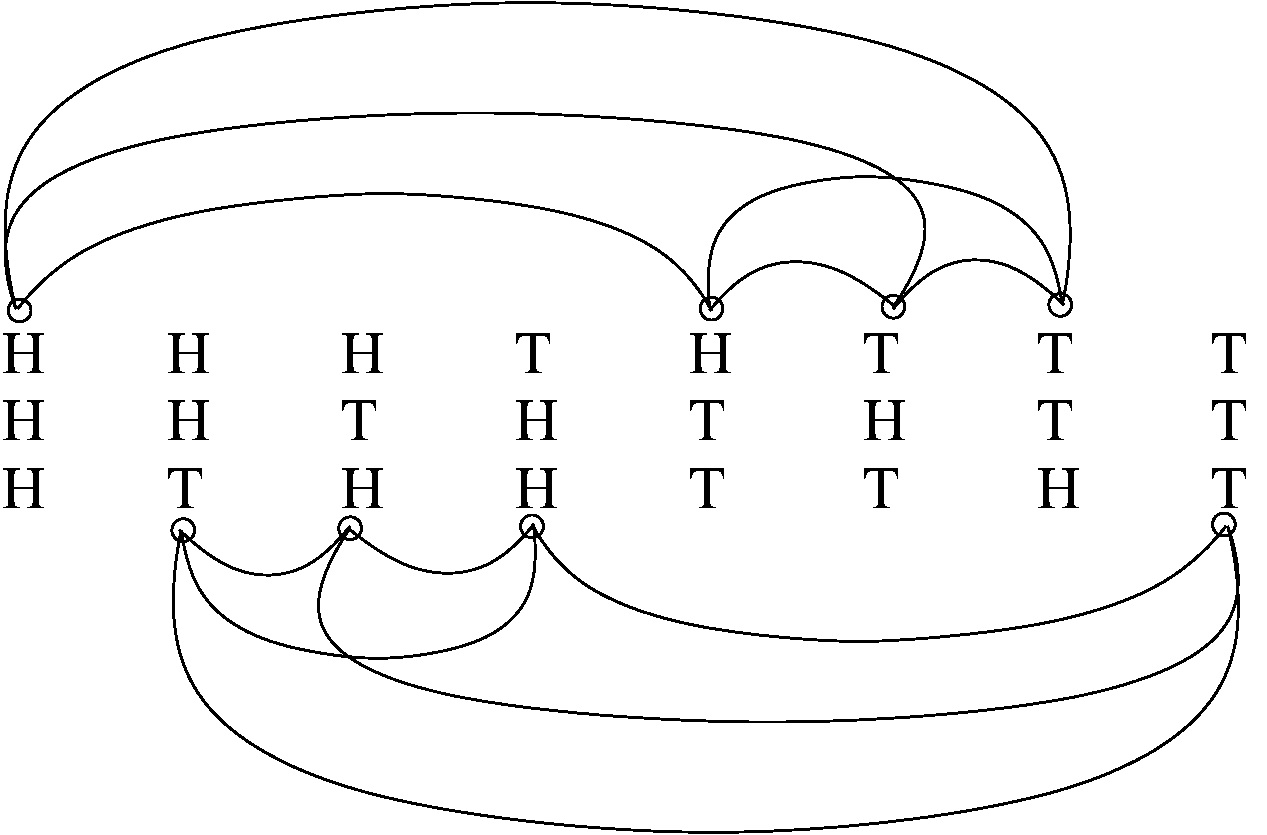
\includegraphics[width=0.5\linewidth,keepaspectratio]{munteneng}
\end{center}
\caption{The 3 coins graph \label{munten}}
\end{figure}

Just looking at the graph shows us that it is impossible to get from
the HHH configuration to the TTT configuration: they belong to a
different component of the graph. The property used here is {\em
reachability}.


%===============================================================================
\section{The Wolf, the Goat, the Cabbage, and the Farmer}

A farmer owns a wolf, a goat and a cabbage. He lives at the left bank
of a river, and he wants to move to the right bank. He also has a
small boat: it is too small to put all his belongings in it at the
same time, in fact, it is so small he can transport at most one
item at a time. He could transport his wolf, goat, and
cabbage to the right bank one by one, in some particular order, but the problem
is that when the wolf and the goat are left alone, the wolf will eat
the goat. Similarly for the goat and the cabbage: they can't be left
alone. So this simple plan does not work. Can the farmer transport all
his belongings to the other side so that nothing gets eaten?

You could of course try out all possibilities - why not try it now!
You notice that there is a problem of bookkeeping while doing that.
A better way is to note down all possible situations: a situation
describes who/what is on which side of the river, and is characterized
completely by what is on the left side. So, the situation FGC means
that the farmer, the goat and the cabbage are on the left bank, while
the wolf is at the right bank. Some situations - like GC - are a
priori forbidden. All situations can be described by the dots in
Figure~\ref{BWGK1}: we use $\ast$ to indicate that nothing is at the
left bank: it is the situation the farmer really wants.

\begin{figure}[ht]
\mbox{
\hspace{1cm}
\subfigure[All possible situations for the farmer, wolf, goat, and
cabbage]{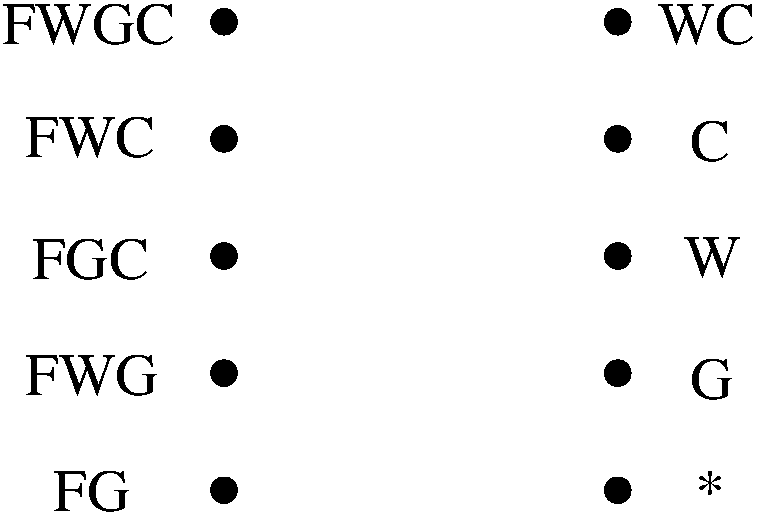
\includegraphics[height=0.12\textheight,keepaspectratio]{BWGK1eng} \label{BWGK1}}\hspace{2.5cm}
\subfigure[The graph describing the situations and their allowed
transitions]{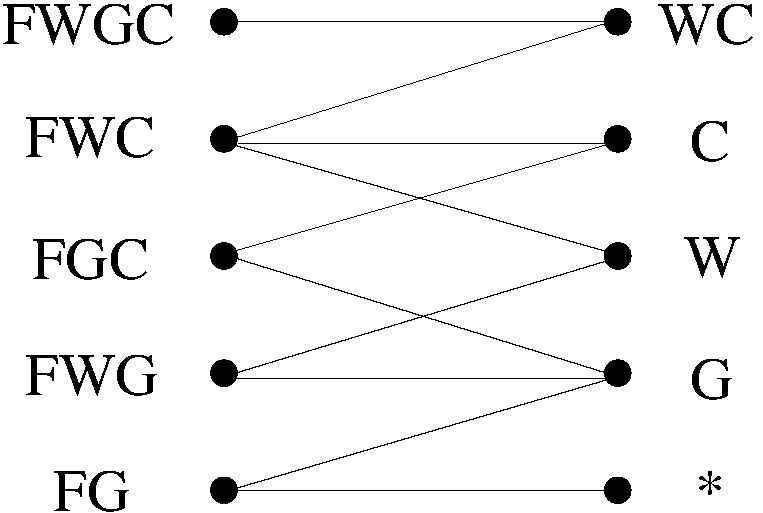
\includegraphics[height=0.12\textheight,keepaspectratio]{BWGK2eng} \label{BWGK2}
} }
\caption{The farmer, wolf, goat and cabbage problem}
\end{figure}

We can now connect any two situations $\alpha$ and $\beta$ if the
farmer can cross the river - possibly with one of his belongings - and
by doing so transforms $\alpha$ into $\beta$. We get the graph in
Figure~\ref{BWGK2}.  The problem is now reduced to the question: is
there a path from vertex FWGC to $\ast$ using the edges in
Figure~\ref{BWGK2}?

Again, reachability is the key concept, and the details of the problem
have been abstracted away.


%===============================================================================
\section{The Bridges of K\"onigsberg}

18$^{th}$ century, K\"onigsberg (now Kaliningrad in Russia): the river Pregel
crosses the city. It contains two islands, connected by a total of 7
bridges with each other and the river banks: see
Figure~\ref{pregel}. The citizens of K\"onigsberg used to make walks
during the weekend, and they wondered: is it possible to make a walk
(starting at home and arriving at home of course) so that every bridge
is crossed exactly once? They couldn't solve it. When the swiss
mathematician Leonhard Euler (1707-1783) visits the town, he hears
about the problem, solves it (negatively), and publishes the first
paper ever on graph theory.

\begin{figure}[ht]
\begin{center}
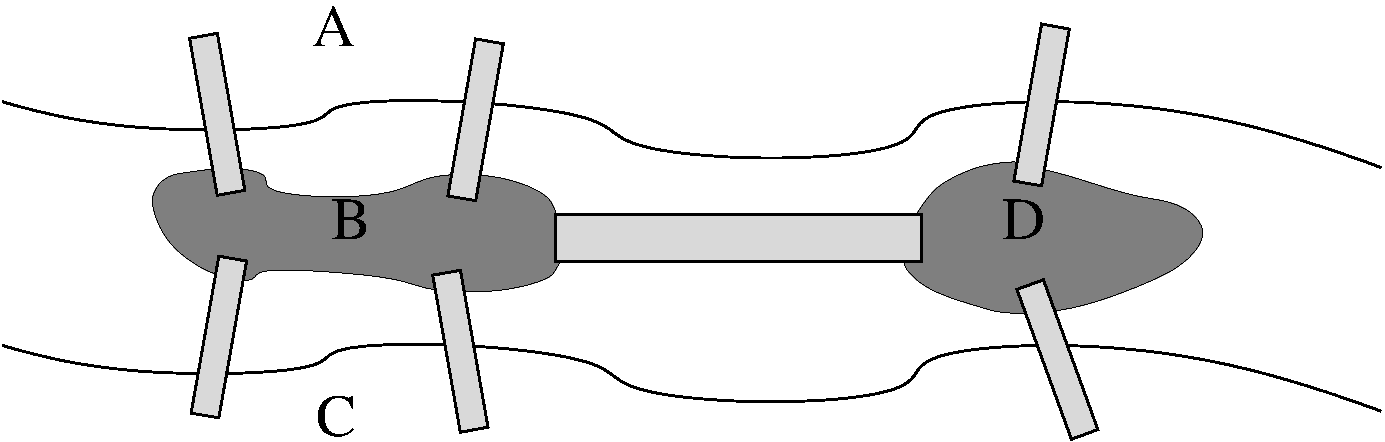
\includegraphics[width=0.4\linewidth,keepaspectratio]{pregel}
\end{center}
\caption{The bridges on the river Pregel \label{pregel}}
\end{figure}

How is this problem connected to graph theory? The graph
representation of the bridges and river banks can be seen in
Figure~\ref{pregelgraph}. The essence of the problem is now: does the
graph have a cycle (a closed path) that uses every edge exactly once?
This kind of cycle is now named an Eulerian cycle. We will later see
that the characterization of graphs with an Eulerian cycle is simple,
as well as finding an Eulerian cycle.

\begin{figure}[ht]
\begin{center}
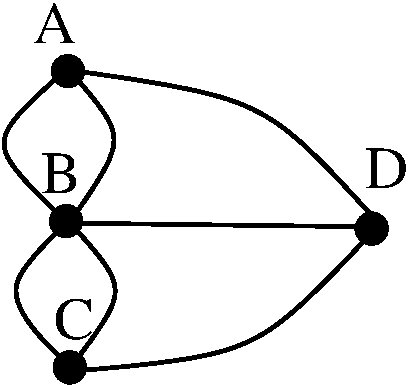
\includegraphics[width=0.15\linewidth,keepaspectratio]{pregelgraph}
\end{center}
\caption{The graph modeling the bridges over the Pregel \label{pregelgraph}}
\end{figure}

You might know the problem of finding an Eulerian cycle (or path) in a
different context: you are given a drawing in which points are
connected by lines; you are asked to draw it by putting your pen at
one point, never lifting it, following all lines not more than once.

Finding Eulerian cycles is important in real life: suppose you need to
check the state of the median strip of the highways. You need to
traverse all highways, but preferably only once.

%===============================================================================
\section{Hamilton's Toy}

Sir William Rowan Hamilton tried to commercialize circa 1850 a 3-D
puzzle in the form of a dodecahedron (it has 12 pentagons):
Figure~\ref{hamilton1} shows a planar representation of this spatial
object. Each corner had the name of a city and the problem consisted
in finding a closed path (a cycle) starting at a particular city so
that every city is visited exactly once. Such path is named a
Hamiltonian cycle. It turns out that finding such a cycle (or proving
it exists) is much more difficult than for Eulerian cycles.

\begin{figure}[ht]
\begin{center}
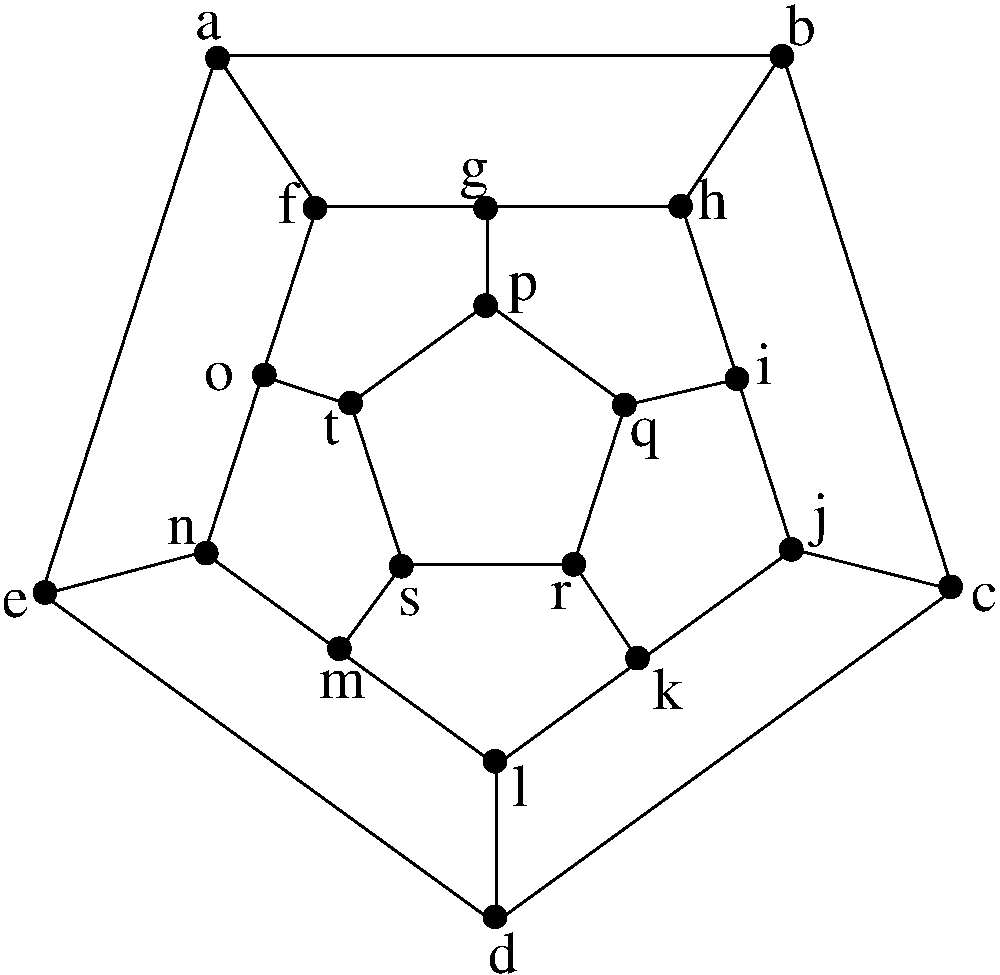
\includegraphics[width=0.4\linewidth,keepaspectratio]{hamilton}
\end{center}
\caption{Hamilton's puzzle
\label{hamilton1}}
\end{figure}

The puzzle was a commercial disaster, but it is at the heart of the
Travelling Salesman Problem \martonst{we will encounter in complexity theory}{}.

The Postman Problem has a similar flavor: during his tour, a postman
wants to visit each street exactly twice (once at each side of the
street) \ldots is that always possible \ldots?

Figure~\ref{hamiltonkring} shows a Hamiltonian cycle for Hamilton's puzzle.

\begin{figure}[ht]
\begin{center}
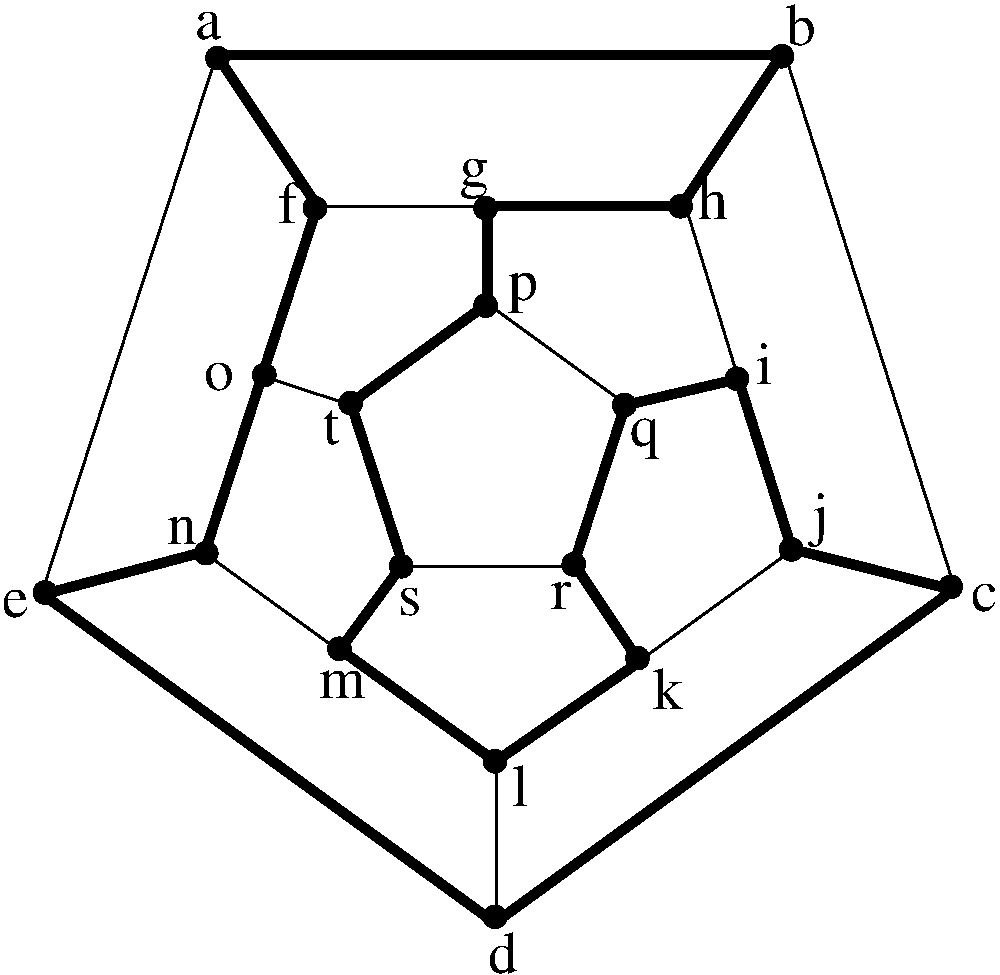
\includegraphics[width=0.6\linewidth,keepaspectratio]{hamiltonkring}
\end{center}
\caption{A solution for Hamilton's puzzle
\label{hamiltonkring}}
\end{figure}

%===============================================================================
\section{References}

\begin{itemize}
\item
Richard Johnsonbaugh ``Discrete Mathematics'', MacMillan, 1984
\item
Shimon Even ``Graph Algorithms'', Pitman, 1979
\item
Ralph P. Grimaldi ``Discrete and Combinatorial Mathematics''
\item
William Barnier, Jean B. Chan ``Discrete Mathematics''
\item
Michael Townsend ``Discrete Mathematics: Applied combinatorics and \\
graph theory''
\end{itemize}



%///////////////////////////////////////////////////////////////////////////////
\chapter{Graphs}

%===============================================================================
\section{Basic Definitions}

\begin{definition}[Graph]
A(n undirected) \textbf{graph} $G$ is a tuple $(V,E)$ in which
$V$ is a set of \textbf{vertices} and $E$ a (multi-)set\footnotemark
of \textbf{edges}; each edge $e \in E$ is an unordered pair $(v,w) \in
V \times V$; we write $e = (v,w)$ or $e = (w,v)$.
\end{definition}

\footnotetext{A \emph{multi-set} is similar to a set, but an element can
occur more than once; $\{1,1,1,2,2,3,4,5,5\}$ is a multi-set.}

We allow some freedom of notation and speech:
\begin{itemize}
\item
we write $G(V,E)$ for the graph $G$ with vertices $V$ and edges $E$
\item
we write $e \in G$ when $e \in E$ and $E$ is a subset of the edges of $G$
\item
we write $v \in G$ when $v \in V$ and $V$ is a subset of the vertices of $G$
\item
let the edge $e = (x,y)$, and $G(V,E)$, then $G \cup \{e\}$ denotes
the graph $(V \cup \{x,y\},E \cup \{e\})$; we say {\em add $e$ to $G$}
\item
let $b$ be an vertex, and $G(V,E)$, then $G \cup \{b\}$ denotes the
graph $(V \cup \{b\},E )$; we say {\em add $b$ to $G$}
\end{itemize}

We assume sometimes that the vertices are numbered from 1 to $n =
|V|$. We will deal only with finite graphs.

Edge is also used in the context of polyhedra, and that is no
surprise: the study of polyhedra and graphs have common points.

Note that $E$ can contain two edges $(v,w)$: we name those edges {\em
parallel}.

An edge $(v,w)$ is {\em incident on} the vertex $v$ (and on $w$);
the vertices $v$ and $w$ are {\em adjacent} to the edge $(v,w)$.

\begin{definition}[Directed graph (digraph)]
A directed \textbf{graph} $G$ is a tuple $(V,E)$ in which
$V$ is a set of \textbf{vertices} and $E$ a (multi-) set
of \textbf{edges}; each edge $e \in E$ is an ordered pair $(v,w) \in
V \times V$; we write $e = (v,w)$.
\end{definition}

You can think of a directed graph as a graph in which each edge has an
arrow, pointing from one vertex to the other.


\begin{definition}[Loop]
  \textup{A \textbf{loop} in a graph is an edge $(v,v)$. }
\end{definition}


\begin{definition}[Simple graph]
\textup{A graph is \textbf{simple} if the graph has neither parallel edges
nor loops.}
\end{definition}


\begin{definition}[Degree of a vertex]
  \textup{The \textbf{degree $\delta(v)$ of a vertex $v$} of graph
$(V,E)$ is the number of edges $(v,w) \in E$, where a loop counts for 2.}
\end{definition}


\begin{definition}[Isolated vertex or point]
A vertex $v$ in a graph $(V,E)$ is {\bf isolated} if $\delta(v)=0$.
\end{definition}


\begin{theorem}[Sum of vertex degrees] \label{somgraad}
The sum of all vertex degrees is even.
\end{theorem}
\begin{proof}
Since each edge $(v,w)$ contributes 1 to the degree of both $v$ as
$w$, each edge contributes 2 to the sum of all vertex degrees, hence
the conclusion.
\end{proof}


\begin{theorem}[Number of vertices with an odd degree]
The number of vertices with an odd degree is even.
\end{theorem}
\begin{proof}
Partition $V$ in the vertices with an even degree $\{a_i |
i=1,\ldots,n\}$, and the vertices with an odd degree $\{b_i |
i=1,\ldots,m\}$.  Then, because of Theorem~\ref{somgraad}
\[0 = \left(\sum_{i=1}^{n} \delta(a_{i}) + \sum_{i=1}^{m} \delta(b_{i})\right)
\bmod 2 = m \bmod 2 \] and the conclusion follows.  \end{proof}


\begin{definition}[Path]
\textup{A \textbf{path} (with length $n$) in a graph $(V,E)$ is a
sequence of edges
\[( e_1=(v_{1},v_{2}),\;e_2=(v_{2},v_{3}),\;\ldots, e_{n}=(v_{n},v_{n+1})).\]
We assume that it is clear which of the parallel edges is used (if at
all important). \\
In a simple graph, a path can also be characterized by a sequence of
vertices $(v_{1}, \ldots , v_{n+1})$}
\end{definition}

\begin{definition}[Simple path]
  \textup{A \textbf{simple path} $(v_{1}, \ldots , v_{n+1})$ is a path
  with the property that $\forall i,j: i \neq j \Rightarrow v_{i} \neq v_{j}$ }
\end{definition}



\begin{definition}[Cycle]
  \textup{A \textbf{cycle} is a path
    $((v_1,v_2),...,(v_n,v_{n+1}))$ such that all edges in it are
different and $v_{1} = v_{n+1}$.}
\end{definition}

A cycle is sometimes called a circuit.


\begin{definition}[Eulerian cycle (path)]
  \textup{An \textbf{Eulerian cycle (path)} is a cycle (path)
containing all edges exactly once.}
\end{definition}

\begin{definition}[Hamiltonian cycle]
  \textup{ A \textbf{Hamiltonian cycle} is a cycle containing all
vertices of the graph exactly once.}
\end{definition}


\begin{definition}[Connected graph]
  \textup{ A graph is \textbf{connected} if for every two different
vertices $v$ and $w$, there is a path from $v$ to $w$.}
\end{definition}



\begin{theorem}[Existence of an Eulerian cycle.]
  A graph $G(V,E)$ has an Eulerian cycle if and only if $G$ is
  connected and the degree of each vertex is even.
\end{theorem}
The intuition behind the proof is that when you arrive in a vertex,
you can leave again because the degree is even. It therefore does not
matter which path you follow, as long as you don't return to the
starting point too soon. Even if you did, you can still mend the path.


\begin{proof}

\begin{itemize}
\item A graph with an Eulerian cycle is connected: the cycle connects
all vertices, so there is a path from each vertex to each other
vertex. While traversing the cycle, we leave every vertex in which we
arrive, and since all edges are traversed by the cycle, the degree of
each vertex is even.

\item Construct a cycle $P$: start from any vertex $s$, follow any
edge incident on $s$; from then on extend the partial path with any
edge incident on the most recently added vertex, never using a
previously used edge. Repeat until there are no more edges to choose
from. Since the degree of each vertex is even, the just constructed
$P$ is a cycle starting in $s$ and arriving at $s$. If $P$ contains
all edges from $G$, the theorem is proven. Otherwise, there exists a
vertex $s'$ on the path $P$ from which an unused edge leaves (explain
why!). Construct a cycle $P'$ starting at $s'$ not using any edges
from $P$ (why is this possible?). Then add $P'$ to $P$: now you have a
larger cycle. One can repeat the procedure until there are no more
unused edges. Figure~\ref{euler4} illustrates the construction.
\end{itemize}
\begin{figure}[ht]
\begin{center}
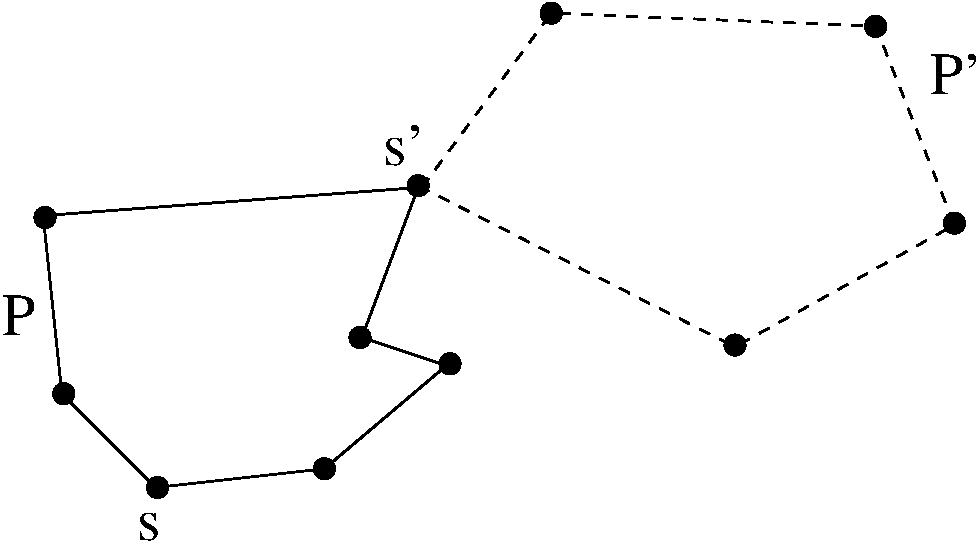
\includegraphics[width=0.4\linewidth,keepaspectratio]{euler4}
\end{center}
\caption{ $P$ and the extension $P'$ \label{euler4}}
\end{figure}
\end{proof}


\begin{theorem}[Existence of an Eulerian path]
  A connected graph $G$ has an Eulerian path from vertex $v$ to $w$
  ($v \neq w$) if $v$ and $w$ are the only vertices with an odd degree.
\end{theorem}
\begin{proof}
Consider the graph $G'$ obtained by adding the edge $(w,v)$ to $G$.
$G'$ is connected and each vertex has an even degree, so it has an
Eulerian cycle $(w,v,\ldots,w)$; delete the first edge from this cycle
to obtain the Eulerian path $(v,\ldots,w)$ in $G$.
\end{proof}

\begin{example}
Looking back at Figure~\ref{pregelgraph} (the graph modeling the
bridges in K\"onigsberg), you notice that there are four vertices with an
odd degree. It follows that there is neither an Eulerian cycle, nor an Eulerian
path.
\end{example}



\begin{definition}[Subgraph]
  \textup{A graph $(V_1,E_1)$ is a \textbf{subgraph} of $(V,E)$ if
    $V_1 \subseteq V$ and $E_1 \subseteq E$.}
\end{definition}



 \begin{definition}[Component of a  graph]
  \textup{A \textbf{component} $C$ of a graph $G$ is a maximal
    connected subgraph of $G$, i.e.
$\forall C' \subseteq G: C \subset C' \Rightarrow C'$ is not connected.}
\end{definition}

 \begin{theorem}[\label{partitie} Partition of a graph]
The components $(V_{i},E_{i})$ ($i=1,\ldots,n$) of a graph $(V,E)$
form a partition,
i.e. \\
$(V,E) = (\cup_{i=1}^{n} V_{i},\cup_{i=1}^{n} E_{i})$ and
for any $i \neq j$, $V_{i} \cap V_{j} = \emptyset$ and $E_{i} \cap E_{j} =
\emptyset$
\end{theorem}
\begin{proof}
Clearly every vertex and edge belongs to at least one component.
Suppose a vertex belongs to two components $\alpha$ and $\beta$, then
the union of $\alpha$ and $\beta$ is a connected subgraph of $(V,E)$
so $\alpha = \beta$, so $V_{i} \cap V_{j} = \emptyset$ for $i \neq
j$. Since an edge belongs to the component of its incident vertices,
the proof can be completed easily.
\end{proof}


Theorem~\ref{partitie} is important because it is often easier to
prove properties for connected graphs: Theorem~\ref{partitie} tells us
that a non-connected graph can be uniquely divided in connected
components.


%===============================================================================
\section{Graph Representations \label{voorstelgraph}}

Until now we have just drawn graphs. However, we often need a more
formal representation of graphs, e.g. because we need to write
programs dealing with graphs. There is no single best representation:
it depends on what we want to compute. So we introduce several
representations, first for undirected graphs, later for digraphs.

Let us number the $n = |V|$ vertices of $G(V,E)$ from 1 to
$n$. Construct an $n\times n$ matrix $A$ with $A(i,j)$ equal to 1 if
$(i,j) \in E$ and 0 otherwise. $A$ is called the adjacency matrix $G$:
it readily shows which vertices are adjacent.

\begin{figure}[ht]
\begin{center}
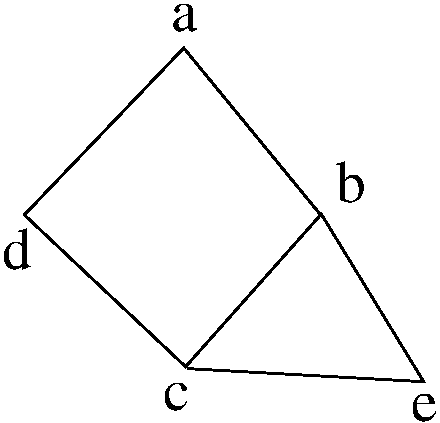
\includegraphics[width=0.15\linewidth,keepaspectratio]{adjacency1}
\end{center}
\caption{ Some graph \label{adjacency1}}
\end{figure}

\begin{example}
The adjacency matrix $A$ of the graph in Figure~\ref{adjacency1} is

\begin{center}
\mbox{\space \space \space}
$\begin{array}{ccccc}
a & b & c & d & e\\
\end{array}
$\\
$
\begin{array}{c}
a\\
b\\
c\\
d\\
e\\
\end{array}
$
$
\left(
\begin{array}{ccccc}
0 & 1 & 0 & 1 & 0\\
1 & 0 & 1 & 0 & 1\\
0 & 1 & 0 & 1 & 1\\
1 & 0 & 1 & 0 & 0\\
0 & 1 & 1 & 0 & 0\\
\end{array}
\right)
$
\end{center}
\end{example}

The adjacency matrix of a simple graph has only zeros on the main
diagonal. The adjacency matrix does not show whether a graph has
parallel edges. The adjacency matrix is symmetric and hence not a
very efficient representation of a graph. Still, it has interesting
properties.

\begin{example}
Compute $A^{2}$ for the example above. We get

\begin{center}
$
A^{2} = \left(
\begin{array}{ccccc}
2 & 0 & 2 & 0 & 1\\
0 & 3 & 1 & 2 & 1\\
2 & 1 & 3 & 0 & 1\\
0 & 2 & 0 & 2 & 1\\
1 & 1 & 1 & 1 & 2\\
\end{array}
\right)
$
\end{center}

We got the $(a,c)$ element of $A^{2}$ by:

\begin{center}
$
\left(
\begin{array}{ccccc}
0 & 1 & 0 & 1 & 0\\
\end{array}
\right)
\times
\left(
\begin{array}{c}
0\\
1\\
0\\
1\\
1\\
\end{array}
\right)
 =
0\times 0 + 1\times 1 + 0\times 0 + 1\times 1 + 0\times 1 = 2$
\end{center}

The positive contributions in the calculation result from the paths
$(a,b)-(b,c)$ and $(a,d)-(d,c)$. This shows that $A^{2}[i,j] = $ the
number of paths from vertex $i$ to vertex $j$ with length 2.
\end{example}
But we need to
be careful: the adjacency matrix does not show parallel edges, and
parallel edges increase the number of paths between two vertices.
As a consequence, the next theorem is about simple graphs.

 \begin{theorem}
\label{aantalpathen}
$ $ \\
Let $A$ be the adjacency matrix of a simple graph $G(V,E)$,\\
then
$A^{n}[i,j] = $ the number of paths with length $n$ from vertex $i$ to vertex
$j$.
\end{theorem}
\begin{proof} We use induction on $n$. For $n=1$, the theorem is true
because of the definition of adjacency matrix.

Suppose the theorem is true for $n$; we prove that the theorem is true
for $(n+1)$: $A^{n+1}=A^{n}*A$, so $A^{n+1}[i,j] = \sum_{k=1}^{\#V}
A^{n}[i,k]*A[k,j]$. By the induction hypothesis, $A^{n}[i,k]$ is the
number of paths from $i$ to $k$, and if there is an edge from $k$ to
$j$, (i.e. if $A[k,j] = 1$), then there are also $A^{n}[i,k]$ paths
from $i$ to $j$ passing through $k$ just before arriving at
$j$. Since no two paths are the same (why not?), the result for
$(n+1)$ follows.
\end{proof}

For the graph in Figure~\ref{adjacency1}, we have
\begin{center}
$A^{4} = \left(
\begin{array}{ccccc}
9 & 3 & 11& 1 & 6\\
3 & 15& 7 & 11& 8\\
11& 7 & 15& 3 & 8\\
1 & 11& 3 & 9 & 6\\
6 & 8 & 8 & 6 & 8\\
\end{array}
\right)
$
\end{center}

You can check manually that the theorem is true.

Making use of the previous result, we can derive that $(\sum_{k=1}^{n}
A^{k})[i,j]$ equals the number of paths from $i$ to $j$ and equal to
or shorter than $n$ edges.

The adjacency matrix can also be used in a different way: interpret
the numbers 0 and 1 as the boolean values $false$ and $true$, and
define boolean matrix multiplication as

\[(A*B)[i,j] = (A[i,1] \wedge B[1,j]) \vee (A[i,2] \wedge B[2,j]) \vee
\ldots \vee (A[i,n] \wedge B[n,j])\]


If $B$ is the boolean adjacency matrix of $G$, then $B^{n}[i,j]$
equals the truth value of the sentence {\em there exists a path of
length $n$ from $i$ to $j$}.

Analogously, $(\sum_{k=1}^{n} B^{k})[i,j]$ (sum means boolean sum,
i.e. $\vee$) is the truth value of {\em there exists a path from $i$
to $j$ of length smaller than or equal to $n$}.

For the usual adjacency matrix, the entries in this sum, for
successive values of $n$, grow indefinitely, but for the boolean
adjacency matrix, the entries can only be $false$ or $true$. Moreover,
they are monotonically increasing, so the limit exists. In fact, the
limit is reached after at most $|V|$ steps, and it is one way to
compute the transitive closure of the relation {\em is connected by an
edge}.

Another graph representation consists of the incidence matrix $I$: it
has a row for each vertex and a column for each edge. $I[i,j] = 1$
iff the $j^{th}$ edge is incident on $i$ and 0 otherwise.  The
incidence matrix of the graph in Figure~\ref{adjacency1} is

\begin{center}
\mbox{\space \space \space}
$\begin{array}{cccccc}
ab & ad & cd & bc & ce & be\\
\end{array}
$\\
$
\begin{array}{c}
a\\
b\\
c\\
d\\
e\\
\end{array}
$
$
\left(
\begin{array}{cccccc}
1 & \hspace{0.18cm} 1 & \hspace{0.18cm}0 & \hspace{0.18cm}0 & \hspace{0.18cm}0 & \hspace{0.18cm}0\\
1 & \hspace{0.18cm}0 & \hspace{0.18cm}0 & \hspace{0.18cm}1 & \hspace{0.18cm}0 & \hspace{0.18cm}1\\
0 & \hspace{0.18cm}0 & \hspace{0.18cm}1 & \hspace{0.18cm}1 & \hspace{0.18cm}1 & \hspace{0.18cm}0\\
0 & \hspace{0.18cm}1 & \hspace{0.18cm}1 & \hspace{0.18cm}0 & \hspace{0.18cm}0 & \hspace{0.18cm}0\\
0 & \hspace{0.18cm}0 & \hspace{0.18cm}0 & \hspace{0.18cm}0 & \hspace{0.18cm}1 & \hspace{0.18cm}1\\
\end{array}
\right)
$
\end{center}

The incidence matrix shows loops and parallel edges.

Instead of using an adjacency matrix, one can also use an {\em
adjacency list}: it is just a list of all edges.


The representation of digraphs can be done as for non-directed graphs:
the adjacency matrix has a 1 on the $(i,j)^{th}$ entry if there is a
directed edge from $i$ to $j$, and otherwise a 0. Usually, this matrix
is not symmetric, but since we never used that fact for non-directed
graphs, Theorem \ref{aantalpathen} applies also to digraphs, and the
idea of the boolean adjacency matrix does too.

One use of the boolean adjacency matrix is in finding out the
functions that are called (directly or indirectly) from a given
function in a given program: you can work that out yourself, and also
discover how you can detect {\em dead code} (compiler jargon),
i.e. functions that are not called by anyone. In Section~\myref{sccs},
this application example is used in an interesting graph algorithm.


%===============================================================================
\section{Graph Isomorphisms}

We do the following experiment: all of you take a pen and paper, and
without looking at what your neighbour is doing, you follow the
following instructions:

\begin{itemize}
\item[]
- draw 5 points and put a name next to each of them \\
- connect the first point you drew with the second point\\
- connect the second with the third\\
- connect the third with the fourth\\
- connect the fourth with the fifth\\
- connect the fifth with the first\\
\end{itemize}

There is a chance that some students come up with one of the graphs in
Figure~\ref{experiment1}.

\begin{figure}[ht]
\begin{center}
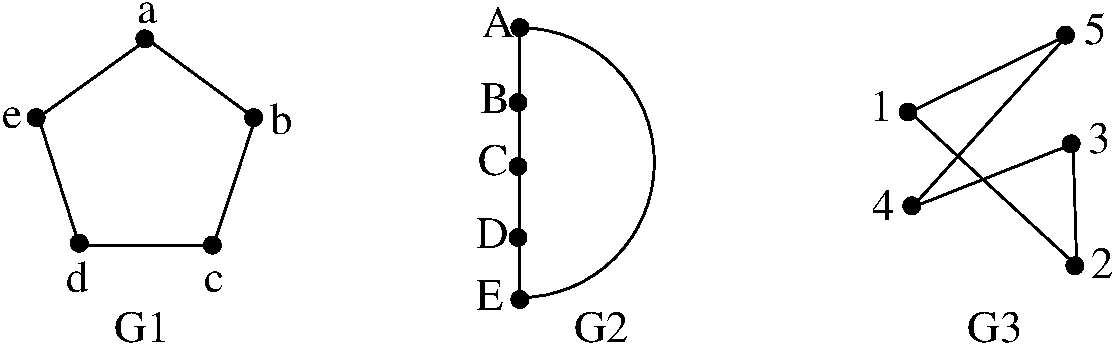
\includegraphics[width=0.6\linewidth,keepaspectratio]{experiment1}
\end{center}
\caption{Three different graphs, or are they equal?\label{experiment1}}
\end{figure}

All these graphs look different, but they were drawn following the
same instructions: there is a good reason for considering them {\em
the same} in some sense, hence the following definition:

\begin{definition}[Graph Isomorphism]\label{isomorfegraphs}
\textup{The graphs $G_{i}(V_{i},E_{i})$ (i = 1,2) are
    \textbf{isomorphic}, if there exists a bijection $f: V_{1}
\rightarrow V_{2}$ such that $g: E_{1} \rightarrow E_{2}$ specified by
$g((v,w)) = (f(v),f(w))$ for all $v,w \in E_{1}$ is well defined,
i.e. $g((v,w)) \in E_{2}$ and a bijection.  Such $f$ is named a
graph isomorphism.}
\end{definition}

Between $G1$ and $G2$ of Figure~\ref{experiment1}, there exists
the isomorphism $f$:
\begin{itemize}
\item[]
f(a) = B\\
f(b) = C\\
f(c) = D\\
f(d) = E\\
f(e) = A
\end{itemize}

You can check that this is a graph isomorphism between $G_{1}$ and
$G_{2}$. Another characterisation of isomorphic graphs relies on the
following theorem:

\begin{theorem}[Characterisation of isomorphic graphs with
the incidence matrix]
Graphs $G_{1}$ and $G_{2}$ are isomorphic if and only if there is an
ordering of the vertices and edges so that the incidence matrices of
$G_{1}$ and $G_{2}$ are equal.
\end{theorem}
\begin{proof}
\begin{itemize}
\item
Let $G_{1}$ and $G_{2}$ be isomorphic, with isomorphism $f$.
Choose any order of the vertices of $G_{1}$. Now order the vertices of
$G_{2}$ by: $f(v) < f(w) \Leftrightarrow v < w$; the order on the
edges of $G_{2}$ is induced in the same way by any order on the edges
of $G_{1}$ and the bijection on the edges. The incidence matrices are
equal.
\item If the incidence matrices are equal, the isomorphism $f$ is
trivial to specify.
\end{itemize}
\end{proof}

We know that the adjacency matrix does not fully determine a graph,
since parallel edges and loops are not visible in the adjacency
matrix. Consequently the following theorem is limited to simple
graphs.

\begin{theorem}[Characterisation of isomorphic simple graphs
with the adjacency matrix]
The simple graphs $G_{1}$ and $G_{2}$ are isomorphic if and only if
there is an ordering of the vertices so that the adjacency matrices of
$G_{1}$ and $G_{2}$ are equal.
\end{theorem}

\begin{proof} Please prove this yourself.
\end{proof}

The theorems on graph isomorphism provide algorithms using the
concrete representation of the graphs. However, every currently known
algorithm for testing whether two graphs are isomorphic is at least
exponential. On the other hand, there exist very efficient tests that
can show that two graphs are {\em not} isomorphic: one checks whether
some graph properties that are {\em invariant} under graph isomorphism
hold for both graphs. Such properties can be based on the number of
vertices, the number of edges, the degrees of the vertices \ldots We will
later see more of such properties. But remember that these simple
tests never tell you that two graphs are isomorphic, only that two
graphs are not isomorphic.



%===============================================================================
\section{Weighted Graphs}

 \begin{definition}[Weighted graph]
  \textup{ A \textbf{weighted graph} $(V,E)$ is a graph in which each
edge $e \in E$ has a \textbf{weight $w(e)$} $\in \R^{+}_0$. The
weight $w(G)$ of a weighted graph $G$, is the sum of the weights of
all the edges of $G$.  }
\end{definition}

The weight of an edge can be interpreted as the length of an
edge, or some cost associated with the use of the edge in a path: if
the graph models a road network, then the weight can be a distance
between cities, or a toll to be paid to use the road. The {\em weight
of a path} is the sum of the weights of the edges in the path. It is
clear that in the case of road networks, one would be naturally
interested in minimal weight paths connecting two given nodes, or put
differently, one is interested in {\em shortest} paths. Since two such
nodes are necessarily in the same component, this section deals with
connected graphs.

The {\em existence} of a shortest path in a connected (and finite)
graph is easy to prove (do it anyway). We are now interested in {\em
constructing} a shortest path. We restrict ourselves to simple graphs:
loops can't occur in a shortest path, and of the parallel edges
between two nodes, we need only the shortest one.

Algorithms in this chapter consist of a sequence of instructions,
numbered 1,2, \ldots . At the end of instruction $n$, there is an
implicit {\bf Go to instruction $n+1$}. {\em Stop} means the algorithm
finishes.


%===============================================================================
\section{Planar Graphs}

Informally, a planar graph is a graph one can draw on a sheet of
paper so that no two edges cross: there is no need for the third
dimension to achieve this non-crossing. There is a formal definition
as well: look it up. We will use the informal definition in proofs.

Another important class of graphs is the class of {\em bipartite}
graphs.

 \begin{definition}[Bipartite graph]
  \textup{A \textbf{bipartite graph} is a graph $(V,E)$ with $V =
V_{1} \cup V_{2}$ so that $V_{1} \cap V_{2} = \emptyset$ and $E
\subseteq V_{1} \times V_{2}$ }
\end{definition}

In words: in a bipartite graph, one can identify two disjoint subsets
of vertices, so that all the edges have an element of each subset as
an endpoint (and consequently, there are no edges that connect nodes
from the same subset).

Figure~\ref{kuratowski1} shows one such graph at the right.

$K_{n,m}$ denotes the bipartite graph in which $|V_{1}| = n$ and
$|V_{2}| = m$, and such that every vertex in $V_{1}$ is connected to
every vertex of $V_{2}$. $K_{n,m}$ occurs naturally when one considers
the problem of connecting $n$ houses with $m$ utilities (water, gas,
electricity, internet \ldots).

$K_{n}$ denotes the graph with $n$ vertices, in which there is an edge
between every two vertex. Such graphs are {\em completely
connected}, and we name them cliques.

The $K$ is in honour of Kazimierz Kuratowski, a famous graph theorist.

Figure~\ref{kuratowski1} shows $K_{4}$ and $K_{2,2}$.

\begin{figure}[ht]
\begin{center}
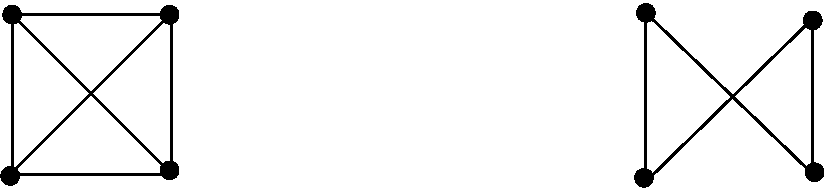
\includegraphics[width=0.4\linewidth,keepaspectratio]{kuratowski1}
\end{center}
\caption{$K_{4}$ and $K_{2,2}$ \label{kuratowski1}}
\end{figure}

When you try drawing $K_{n}$ on paper for successive values of $n$,
and such that no two edges cross, you notice that from $n=5$ on, it is
no longer possible. Similarly, trying this for successive values of
$(n,m)$ and $K_{n,m}$, it fails for all $n,m > 2$.

As we said before, graphs one can draw in the plane without crossing
edges are named \textbf{planar}. As an application: if the graph of a
road network is planar, there is no need for tunnels or bridges. Euler
proved the following formula in 1752\footnote{Descartes
($\pm$ 1600) knew the formula and most probably so did Archimedes
($\pm$ --250)}:

 \begin{theorem}[Euler's formula for planar graphs:]
If $G$ is a connected planar graph with $e$ edges, $v$ vertices and
$f$ {\em faces} then $v-e+f = 2$.
\end{theorem}

We haven't defined a face yet: informally, it is a piece of the plane
enclosed by a minimal cycle. The infinite part of the plane
that lies outside of a (drawing of a) graph also counts as a face. The
origin of the word {\em face} is in the study of polyhedra.


\begin{proof} We use induction on the number of edges. Suppose
$e=1$. Then $G$ is one of the graphs in Figure~\ref{euler1}. In
both cases, the Euler's formula is correct.  Suppose the formula is
correct for all graphs with $n$ edges. Let $G$ be a graph with $(n+1)$
edges.

\begin{figure}[ht]
\begin{center}
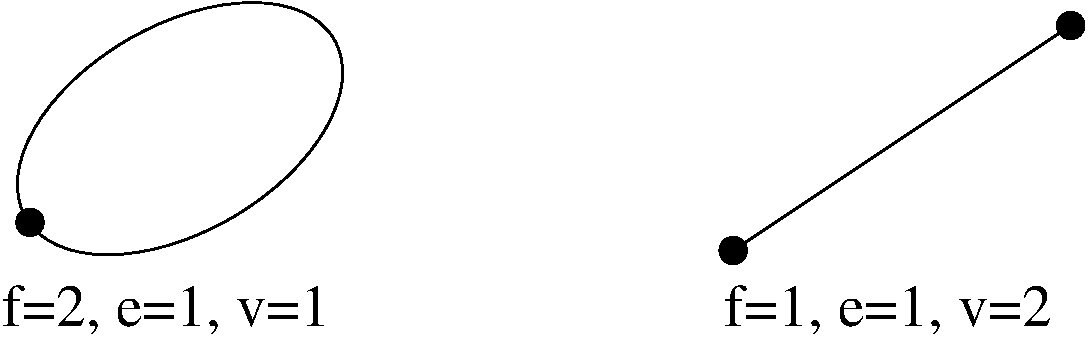
\includegraphics[width=0.4\linewidth,keepaspectratio]{euler1}
\end{center}
\caption{The two graphs with $e=1$ \label{euler1}}
\end{figure}

1) First assume that $G$ does not contain a cycle. Consider a maximal
simple path in $G$; that path contains a vertex $a$ with $\delta(a) =
1$: now consider the graph $G'$ which you obtain by removing from $G$
the vertex $a$ and the only edge arriving there; $G'$ has 1 vertex
and 1 edge less than $G$, the same number of faces, and $G'$ is also
connected (why?), so Euler's formula is valid for $G'$, and
consequently also for $G$ (see e.g. Figure~\ref{euler2}).\\
\begin{figure}[ht]
\begin{center}
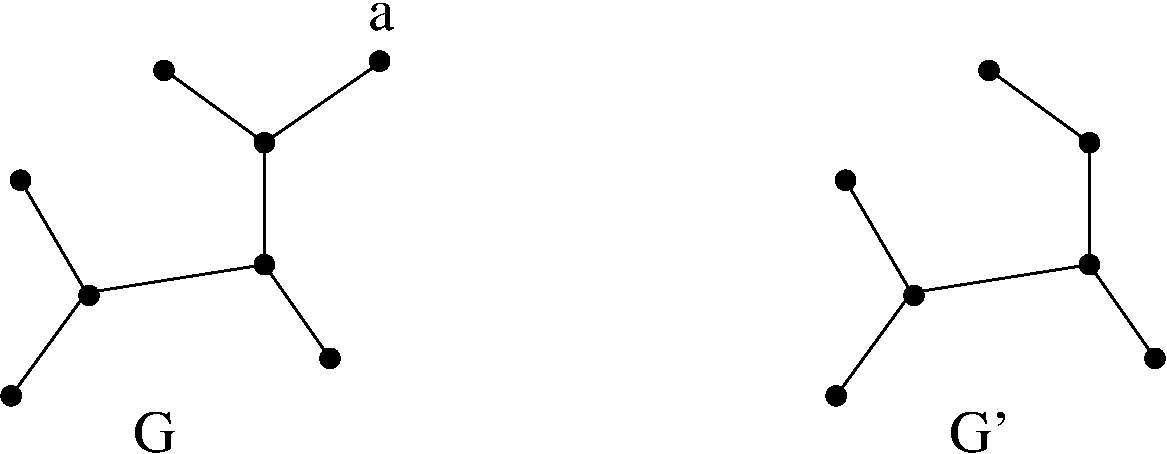
\includegraphics[width=0.4\linewidth,keepaspectratio]{euler2}
\end{center}
\caption{G without a cycle \label{euler2}}
\end{figure}

2) Suppose now that $G$ contains a cycle: take away any edge $x$ from
this cycle, but not its endpoints; the result is $G'$ (see
e.g. Figure~\ref{euler3}).
\begin{figure}[ht]
\begin{center}
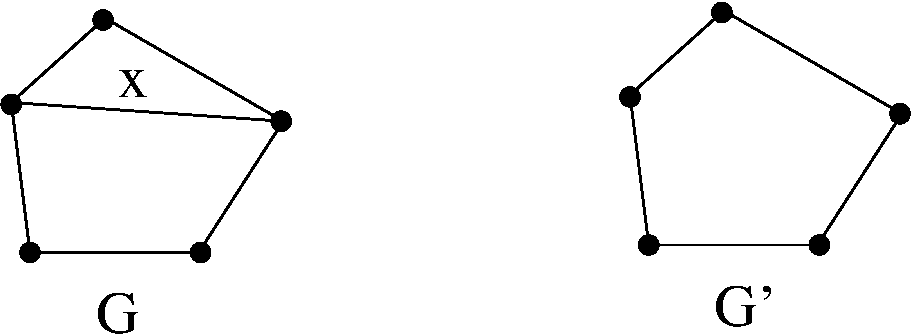
\includegraphics[width=0.4\linewidth,keepaspectratio]{euler3}
\end{center}
\caption{$G$ with a cycle \label{euler3}}
\end{figure}
$G'$ has $n$ edges, the same number of vertices as $G$, and one less
face than $G$; $G'$ is connected (why?); so Euler's formula is valid
for $G'$ (by the induction hypothesis), and it follows that Euler's
formula is also valid for $G$.
\end{proof}

Note that the connectedness condition is essential: the graph with two
vertices and no edge, has $f = 1, e = 0, v = 2$, so Euler's formula is
not valid. You should be able to generalize Euler's formula to
non-connected graphs, taking into account the number of components.

The origin of Euler's interest in this formula lies in the study of
spatial objects, more specifically polyhedra. This interest
existed already since Greek ancient history: regular polyhedra were
supposed to be the building blocks of the world. The formula expresses
the relation between the number of faces, edges and vertices of a
polyhedron. The transformation from a polyhedron and a planar graph
can be visualised as follows: imagine the polyhedron is drawn on a
balloon. Carefully make a hole in the middle of any face, and stretch
the hole until all the material is in a plane. The resulting picture
of edges and vertices form a planar graph. The face that was punctured
corresponds to the infinite face.

 \begin{theorem}
$K_{3,3}$ and $K_{5}$ are not planar.
\end{theorem}
\begin{proof}
Suppose $K_{3,3}$ is a planar graph. Let $\beta$ be the total number
of edges in all faces: an edge counts $n$ times if that edge occurs in
$n$ faces. Since (in a planar drawing) every edge can belong to at most 2
faces, we know that $2*e \geq \beta$.

Moreover, every cycle in $K_{3,3}$ has at least 4 edges (why?) from
which it follows that $\beta \geq 4*f$. Together with the previous
inequality, we derive $e \geq 2*f$. Now use Euler's formula to
eliminate $f$ from the right hand side. We get $e \geq 2*(e-v+2)$.
Fill out the values for $e$ and $v$ for $K_{3,3}$, and get $9 \geq
10$, which is not true. So $K_{3,3}$ is not planar.

Every cycle in $K_{5}$ has minimally 3 edges \ldots\ and the rest of
the proof is like above.
\end{proof}


When two graphs are isomorphic, they are basically the same up to a
renaming of the vertices. But graphs sometimes look similar even
though they they do not have the same number of edges or
vertices. E.g. if we add a vertex in the middle of an edge, it feels
like nothing essential has changed in the graph. For one thing, its
planarity has not changed, neither its connectivity (and you may
perhaps think of other properties that remain invariant). The
operation of adding the extra vertex is named subdivision or expansion
of the graph. The inverse operation is named {\em smoothing (out)} the
graph. The latter consists of replacing two edges $(a,b)$ and $(b,c)$
of which $\delta(b) = 2$ by one edge $(a,c)$. See Figure~\ref{rij1}.



\begin{figure}[ht]
\begin{center}
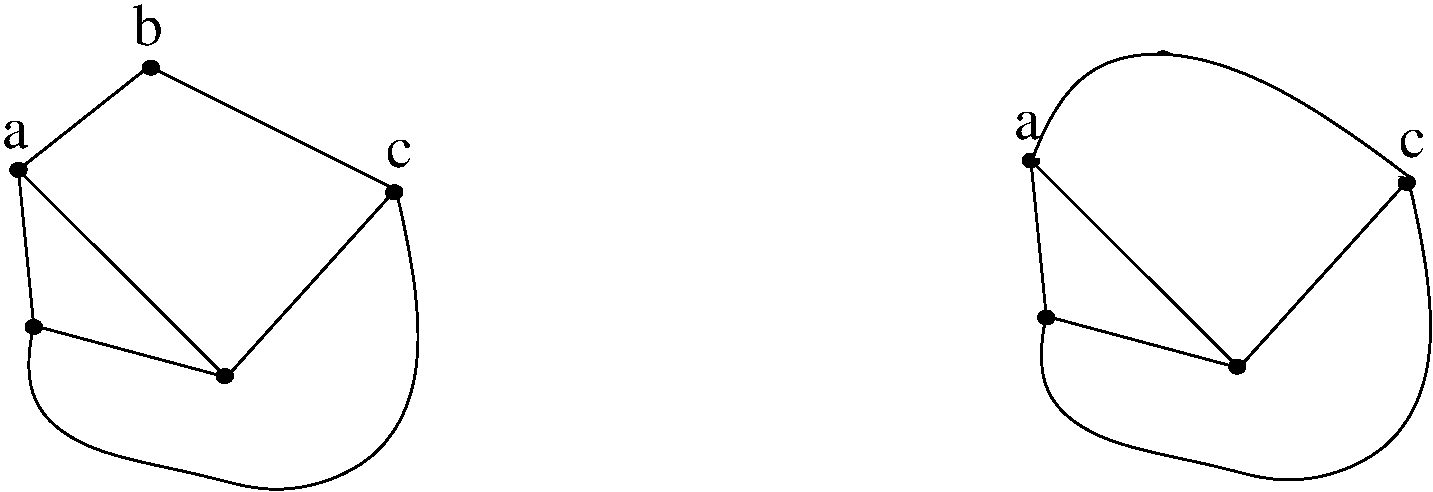
\includegraphics[width=0.4\linewidth,keepaspectratio]{rij1}
\end{center}
\caption{Smoothing a graph \label{rij1}}
\end{figure}

\begin{definition}
  \textup{Two graphs $G_{1}$ and $G_{2}$ are \textbf{homeomorphic} if
by applying smoothing to both graphs, one obtains isomorphic graphs.}
\end{definition}

 \begin{theorem}[Kuratowski's Theorem]
A graph is planar if and only if it does not contain a subgraph
homeomorphic to $K_{5}$ nor $K_{3,3}$.
\end{theorem}
\begin{proof}
One direction is obvious (but please give arguments!). The other direction
is out of the scope of this course.
\end{proof}

The above theorem basically says that $K_{5}$ and $K_{3,3}$ are in
some sense the smallest non-planar graphs.


%===============================================================================
\section{Graph Coloring}

 \begin{definition}
\textup{A \textbf{coloring} of a graph $(V,E)$ is an assignment of a
  color to each $v \in V$ such that the colors of $v$ and $w$ differ
  if $(v,w) \in E$. An
  \mbox{\textbf{n-coloring}} is a coloring with $n$ or less
  (different) colors. A \textbf{minimal} coloring is an $n$-coloring
  with minimal $n$.}
\end{definition}

There are lots of practical applications of (minimal) graph colorings.
Just a few examples:

\begin{itemize}
\item
Suppose you need to plan 4 meetings, involving persons A,B,C and D. The
first meeting must be attended by A and B; the second by A and C; the
third by B, C and D, and the fourth one by C and D. What is the
minimal number of time slots you can make all these meetings happen?
You may assume you have enough meeting places, and that each meeting
takes the same time. Of course, a person can't attend two meetings at
the same time.

You can represent this problem by the graph in Figure~
\ref{planning1}: each vertex corresponds to a meeting, and two
meetings are connected if they can't be at the same moment (because
some person needs to attend both). Now find a minimal coloring of this
graph, et voil\'{a}! Each color corresponds to a new time slot.
\begin{figure}[ht]
\begin{center}
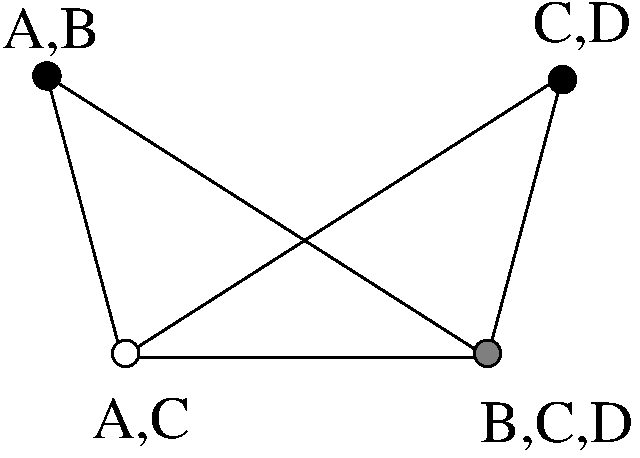
\includegraphics[width=0.2\linewidth,keepaspectratio]{planning1}
\end{center}
\caption{The meeting graph with a minimal coloring\label{planning1}}
\end{figure}

\item
You need to organize the goods in a supermarket on the racks, but some
goods can not be put next to each other, e.g. fuel can't be next to
bread, porn not next to cleaning powder, etc. Once more, you can
construct a graph representing the constraints, and a coloring of the
graph solves your problem.

\item
A compiler tries to put integer variables in machine registers
instead of in memory (why?). There are typically more variables than
available registers, but the same register can be used for more than
one variable. For example, consider the following code:


\parbox{9cm}{
\begin{tabbing}
123 \= 1234 \= 12 \= 12 \= 12 \kill
\> \> \{\\
\> \> \> int i,j,k,l,m;\\
\\
\> \> \> i = 1;\\
\> \> \> j = 2;\\
\> \> \> k = i+j;\\
\> \> \> i = 3;\\
\> \> \> j = 4;\\
\> \> \> l = i+j;\\
\> \> \> m = k+l;\\
\> \> \}
\end{tabbing}
}\\

$i$ and $l$ can be assigned the same register, and likewise for $k$
and $m$. You can find that out by constructing the inference graph of
this piece of code: the graph has the variables as vertices, and an
edge between two variables whose value is {\em alive} at the same
moment. Figure~\ref{regalloc1} shows the corresponding graph.

\begin{figure}[ht]
\begin{center}
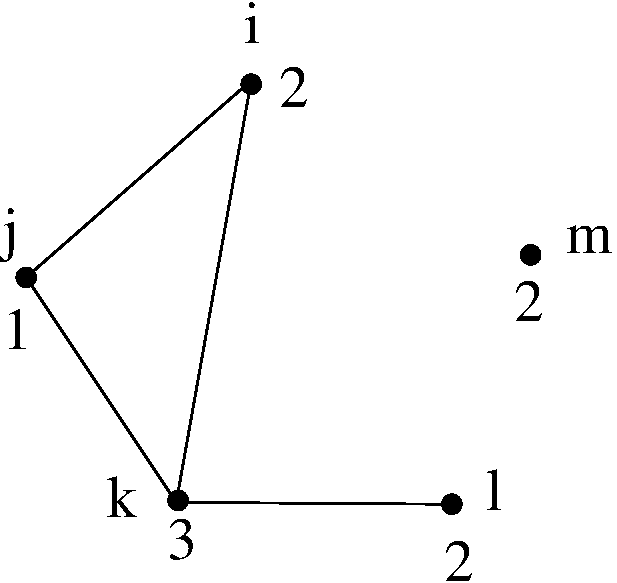
\includegraphics[width=0.2\linewidth,keepaspectratio]{regalloc1}
\end{center}
\caption{The interference graph and a coloring (with numbers) \label{regalloc1}}
\end{figure}

A minimal coloring determines the minimal number of registers needed
to assign each variable in a register, and also an optimal assignment.

\end{itemize}

A problem with practical implications, and historically important, is
the 4-color problem: is it possible to color each map with four
colors, so that no two neighboring countries have the same color? This
problem was set up by Francis Guthrie around 1850, and conjectured to
have a positive answer. Despite several attempts, the conjecture
remained unproven until 1976: K. Appel and W. Haken proved that there
exist 1936 graphs of which at least one must be in any 4-colorable
graph, and then proved that such graphs are not minimal ... The proof
was performed by a computer program.

The connection between map coloring and graph coloring is rather easy
for planar graphs. A map is a planar graph $G$, and can be turned into
another planar graph - its {\em dual} - $G'$ as follows: assume for
the sake of simplicity that each region in the map is a country. Each
country has a capital inside that country. Now construct the graph
with the capitals as nodes, and define an edge between two capitals if
their countries share a border. Figure~\ref{dual1} shows some
examples.


\begin{figure}[ht]
\begin{center}
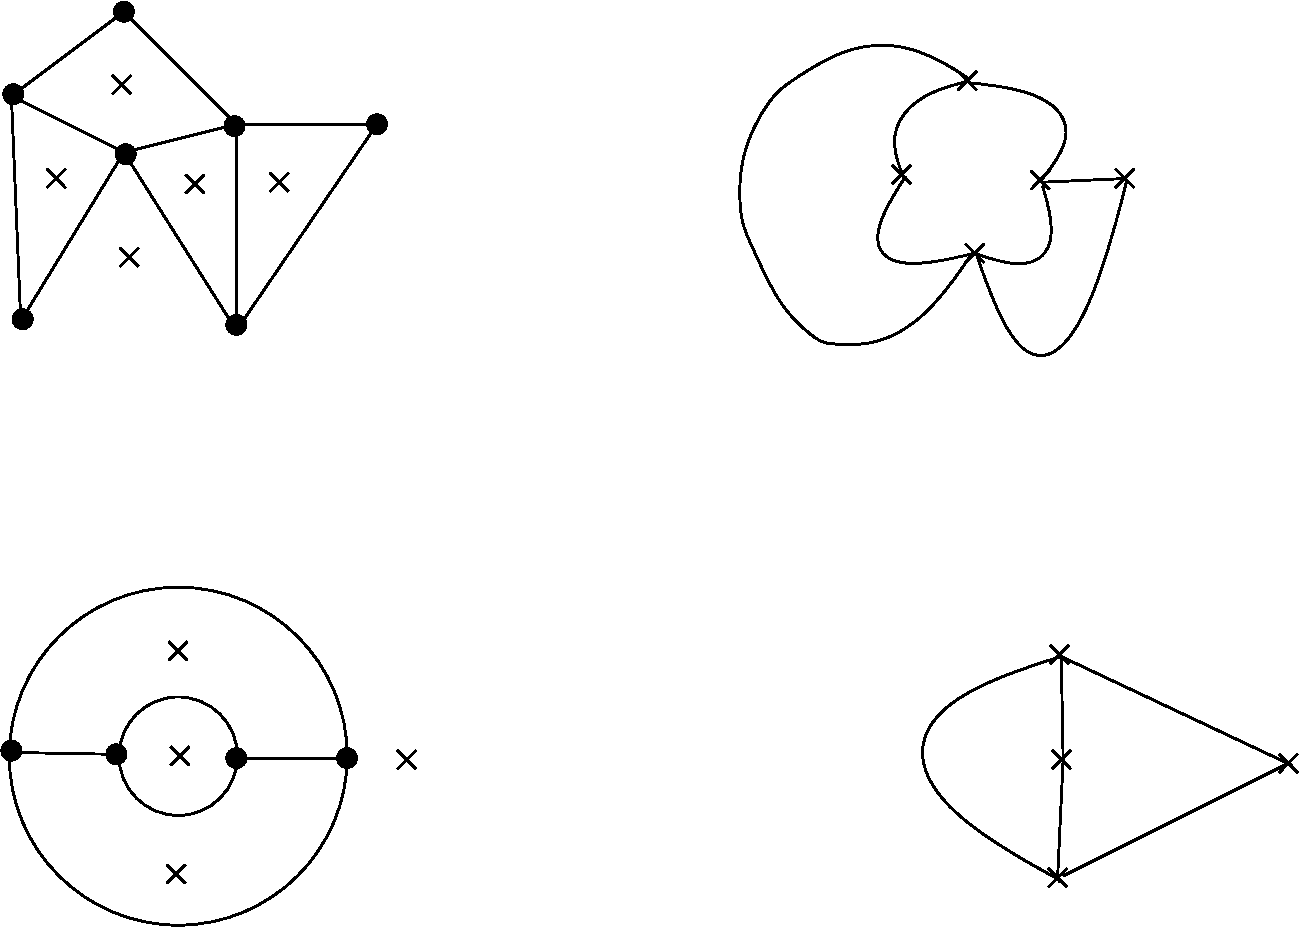
\includegraphics[width=0.6\linewidth,keepaspectratio]{dual1}
\end{center}
\caption{Two planar maps and their dual graphs\label{dual1}}
\end{figure}

Note that the dual graph of a planar map is planar, and simple. A
coloring of the dual graph, corresponds to a coloring of the map - and
vice versa.

In the rest of this section, we prove the 5-color theorem: every
planar graph can be colored with 5 colors.

 \begin{theorem} $e \leq 3*v-6$ for every planar, simple graph
     $G$ with more than one edge.\label{euler}
\end{theorem}
\begin{proof}
We prove the theorem only for connected graphs: first remove
every vertex from $G$ with a degree of 1 (and the corresponding edge),
until no more such vertices exist. The resulting graph $G'$ is still
planar, simple and connected. Denote the number of its edges by $e'$,
the number of its vertices by $v'$; the number of faces is $f$
because removing the particular edges did not change that. So we have
$e-e'=v-v'$ which is equal to the number of removed edges (or
vertices). Denote that quantity by $t$. We now make a case distinction:

1) if $e' = 0$ then $v' = 1$; since $e > 1$ we also have $t > 1$;
so we know: $e = t$ and $3*v-6 = 3*(v'+t) -6 = 3*t-3$; since $t \leq
3*t-3$, we get $e \leq 3*v-6$.

2) $e'$ can't be equal to 1 or 2 (why not?)

3) $e' > 2$; every face is delimited by at least 3 edges (because
there are no loops or parallel edges); let $\sum$ denote the sum of
the number of edges in all faces. then $\sum \geq 3*f$; since each
edge borders exactly 2 faces (why?), we also have $\sum = 2*e'$, so
$2*e' \geq 3*f$. Now use Euler's formula for $G'$ to eliminate $f$
from this inequality, and you get: $e' \leq 3*v'-6$ and thus $e'+t
\leq 3*(v'+t)-6$ and $e \leq 3*v-6$.
\end{proof}

 \begin{theorem} A planar, simple graph has at least one
 vertex - say $v$ - with $\delta(v) \leq 5$.
\end{theorem}
\begin{proof}
This is clearly true for graphs with 1 or 2 vertices. Suppose the
theorem is not true for a certain graph with at least 3 vertices,
i.e. this graph has degree at least 6 for each vertex. Then the sum of
the degrees of all the vertices is at least $6*v$, so, $e \geq 3*v$,
in contradiction with the $e \leq 3*v-6$ from the previous theorem.
\end{proof}

We are now ready to state and prove

 \begin{theorem} 5 colors is enough to color any simple,
     planar graph $G(V,E)$.
\end{theorem} % uit Townsend
\begin{proof} (the proof follows Townsend)

We use induction of the number of vertices: a $G$ with just one vertex,
can clearly be colored with 5 colors. Also, assume $G$ is connected:
if not, the theorem will be proven true for its components, and carry
over to the whole graph. So, assume that the theorem is true for
graphs with $n$ vertices; let $G$ have $n+1$ vertices. Then there is
at least one vertex $v$ with degree 5 or less.

1) If $v$ has degree 4 or less, then $v$ occurs in $G$ as in
Figure~\ref{5kleuring1}.

\begin{figure}[ht]
\begin{center}
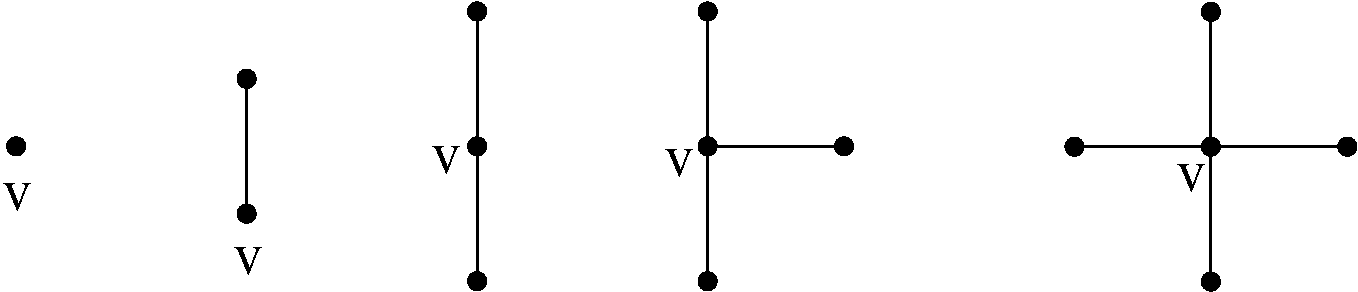
\includegraphics[width=0.6\linewidth,keepaspectratio]{5kleuring1}
\end{center}
\caption{The 5 possibilities in which $\delta(v) < 5$ \label{5kleuring1}}
\end{figure}

Consider the $G'$ obtained by deleting $v$ from $G$ (and the edges
arriving in $v$). $G'$ has the required properties for the theorem,
and it has only $n$ vertices, so by the induction hypothesis, it has a
$5$-coloring. Since $v$ has at most 4 neighbors, $v$ can get a color
different from the color of all its neighbors, resulting in a
$5$-coloring of $G$.

2) If $\delta(v) = 5$, then $v$ occurs in $G$ as in
Figure~\ref{5kleuring2}: each neighbor $w_{i}$ of $v$ has a color
$c_{i}$ ($i = 1,\ldots,5$) as obtained by a $5$-coloring of $G'$.

\begin{figure}[ht]
\begin{center}
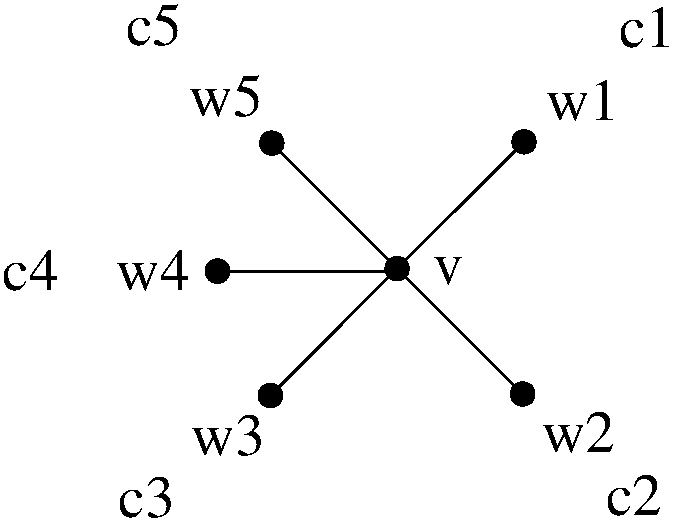
\includegraphics[width=0.25\linewidth,keepaspectratio]{5kleuring2}
\end{center}
\caption{$\delta(v) = 5$ \label{5kleuring2}}
\end{figure}

We still need to determine a color for $v$. If the neighbors of $v$ do
not use all 5 colors, we can give $v$ any remaining color.

So, assume that all five $c_{i}$ are different. Consider the set
$P_{1,3}$ of all paths in $G'$ starting at $w_{1}$ and whose vertices
have alternating colors $c_{1}$ and $c_{3}$. We name such paths
$c_{1}-c_{3}$ paths.  There are two possibilities:

\begin{description}
\item[$P_{1,3}$ does not contain a path that contains $w_{3}$:]
  for each vertex in the paths $P_{1,3}$, change color $c_{1}$ in
  $c_{3}$ and vice versa. We obtain a different $5$-coloring of $G'$
  (why?) and now vertices $w_{3}$ and $w_{1}$ have the same color
  $c_{3}$, so $v$ has no neighbor with color $c_{1}$. This means the
  new 5-coloring of $G'$ can be extended to a $5$-coloring of $G$, by
  assigning $v$ the color $c_{1}$.

\item[$P_{1,3}$ contains a path $p_{1,3}$ that contains $w_{3}$:]
  construct the path set $P_{2,5}$; as you can see in
  Figure~\ref{5kleuring3}, $P_{2,5}$ cannot contain a path that
  contains $w_{5}$; indeed, if such a path $p_{2,5}$ exists, then both
  $p_{1,3}$ and $p_{2,5}$ can be extended with the vertex $v$ so that
  they form cycles in $G$; these cycles must intersect, but not in a
  vertex, because of the different colors. But we have started from a
  plane drawing of the graph, so no intersection is possible. This
  means that no path in $P_{2,5}$ arrives at $w_{5}$, and we can use
  the trick.
\end{description}

\begin{figure}[ht]
\begin{center}
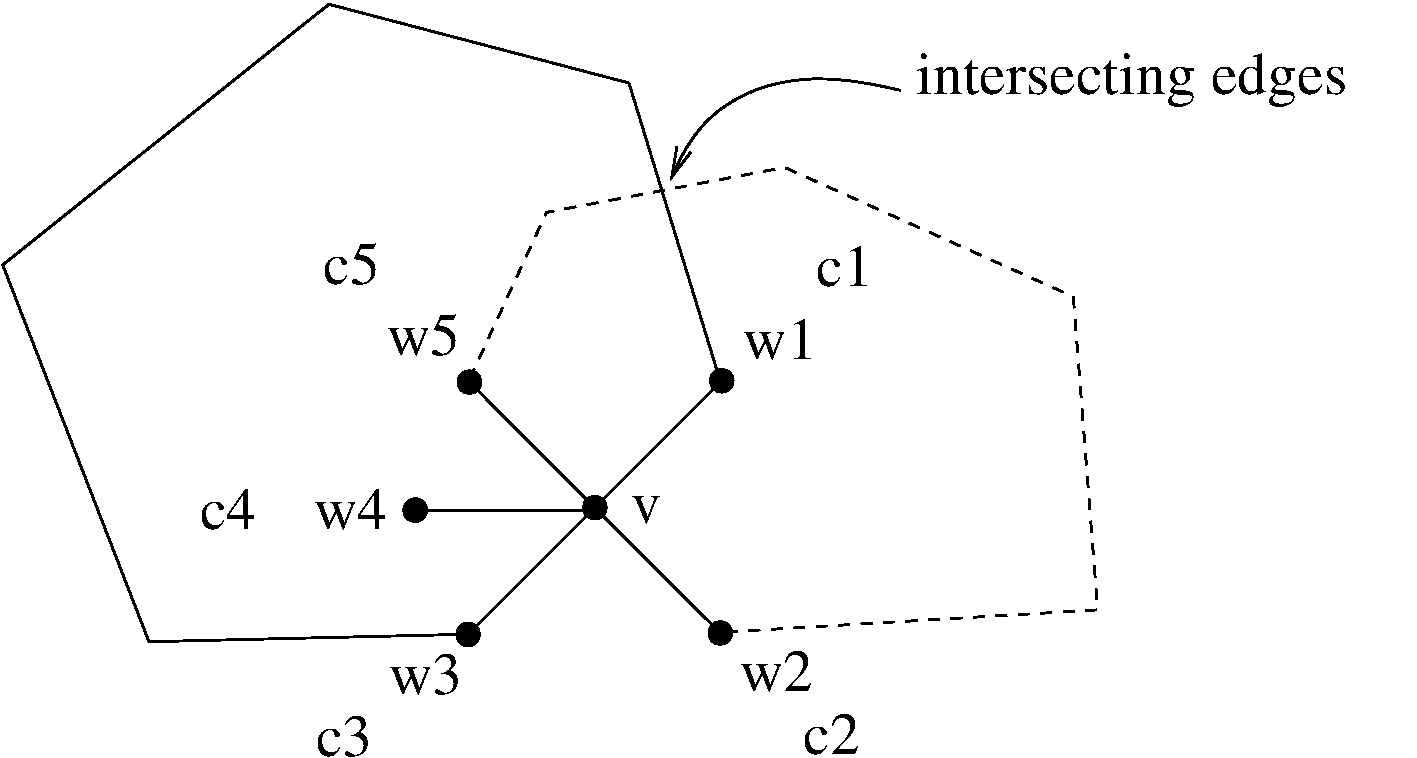
\includegraphics[width=0.4\linewidth,keepaspectratio]{5kleuring3eng}
\end{center}
\caption{$p_{1,3}$ and $p_{2,5}$ \label{5kleuring3}}
\end{figure}
\end{proof}

Appel and Haken {\em proved} that every planar graph has a
$4$-coloring, so they {\em proved} the 4-color conjecture for planar
maps.

This is a good moment to reflect on the concept of a {\em computer
  proof}. Whether something is accepted as a proof or not, is mainly a
social given. It feels true that the mathematical correctness of a
proof is independent of people agreeing with it, but a proof exists
mainly by the grace of the community accepting the proof, even if the
proof turns out to be incorrect later. So it is up to the community
(only to the mathematical community?) to accept or reject computer
proofs: one could imagine a branch of science that accepts only hand
written proofs on paper, just as there is a branch of mathematics that
accepts only constructive proofs, and no existential proofs. It is not
possible to decide unequivocally whether to accept computer proofs just
based on scientific arguments. But the fact is that the proofs are
only possible by computer, the more we are inclined to accept such
proofs, especially if the theorems so proven have useful consequences.

One could argue that it is in principle possible to check a computer
proof by hand, or prove (by hand) that the computer program generating
the proof is correct. That is currently not possible for larger
programs. Moreover, one would also have to prove the correctness of
the machine executing the program \ldots something we might want to
leave to another computer program?

Returning to the coloring of graphs: there are non-planar graphs with
no 4-coloring, e.g. $K_{n}$ with $n > 4$ needs at least $n$ colors,
and the same holds for graphs containing the clique $K_n$. But there also
exist graphs not containing $K_4$ (or larger) with no
3-coloring. Finally, lots of non-planar graphs have a 4-coloring. More
specifically, every bipartite graph (e.g. $K_{3,3}$) has a 2-coloring.


%===============================================================================
\section{Strongly Connected Components}\label{sccs}

We abbreviate {\em strongly connected component} to SCC. Robert Endre
Tarjan \footnote{Turing award 1986} - the master algorithmist -
designed a very nice algorithm in 1972 that partitions the vertices of
a digraph into SCCs. An SCC is a (maximal) set of vertices in which
every node is connected to every other node of the same set. We first
look at an application. Below is a program in pseudo-code, from which
everything is stripped except the procedure call and definitions.

\begin{Verbatim}[frame=single, samepage=true, fontsize=\scriptsize]
main()               venus()                aurochs()           tarpan()
{ venus();           { pluto();             { dodo();           { aurochs();
  aurochs();           venus();               tarpan();         }
}                    }                      }

                     pluto()                dodo()              mamoet()
                     { venus();             { tarpan();         { mamoet();
                     }                        mamoet();         }
                                            }
\end{Verbatim}
The {\em call graph} of this program can be seen in
Figure~\ref{vbtarjan}: the vertices are the procedures; there is a
directed edge $(p_1,p_2)$ if and only if $p_1$ calls $p_2$. We have
left out the self-calls.

% \clearpage

\begin{figure}[h]
\begin{center}
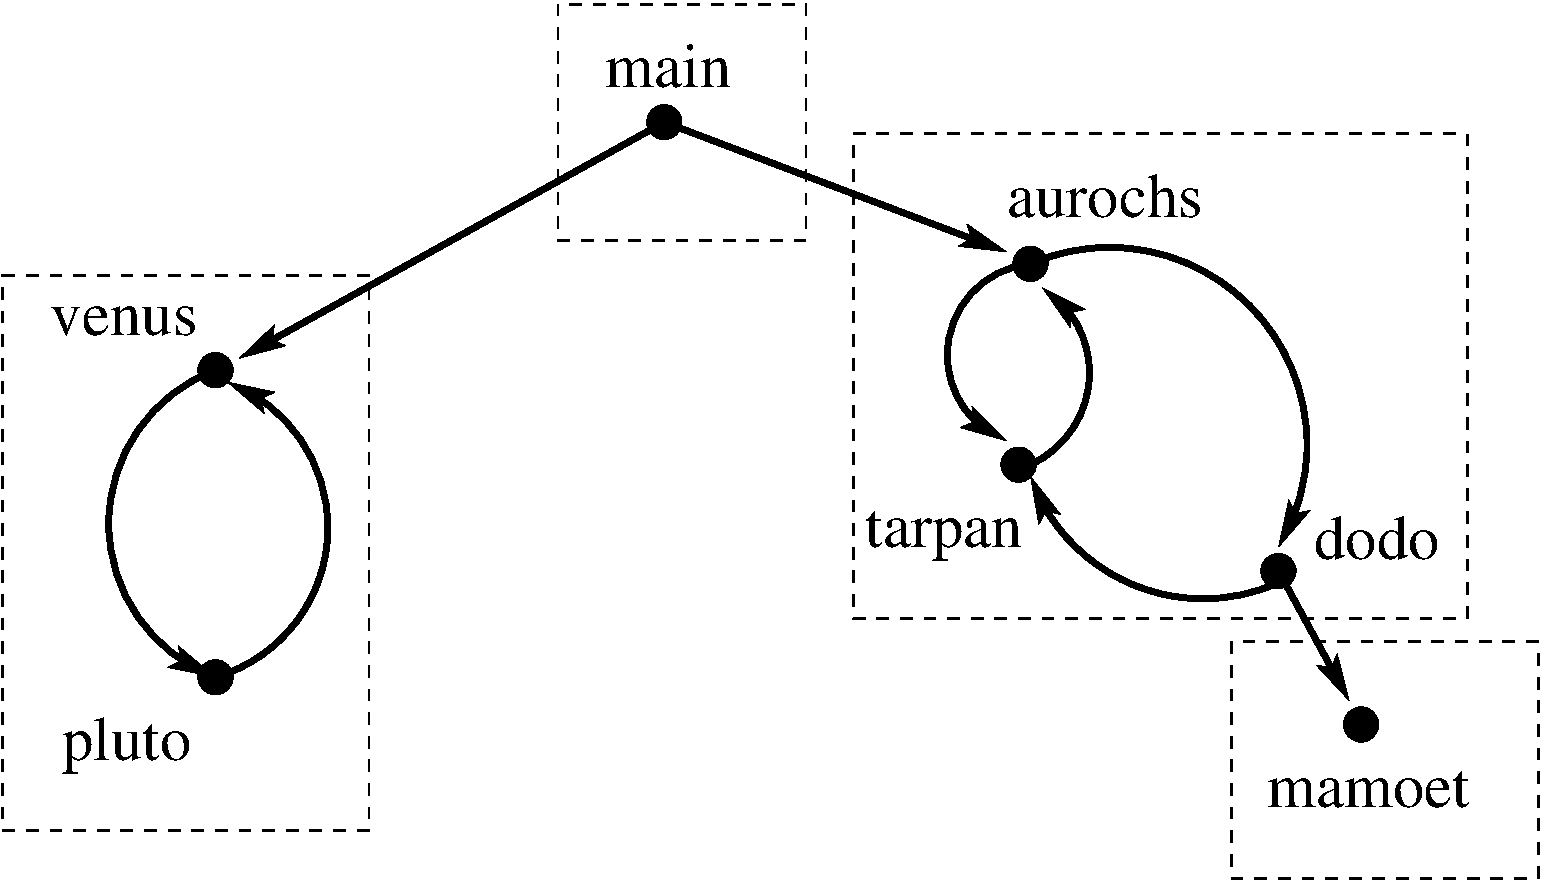
\includegraphics[height=0.2\textheight,keepaspectratio]{vbtarjan}
\caption{The directed call graph}\label{vbtarjan}
\end{center}
\end{figure}

SCCs partition the program in smaller parts of which the analysis can
be performed independently, and/or sequentialized
appropriately. The analysis could concern complexity, invariants (for
correctness), data-flow, liveness analysis (for optimization) ... One
finds uses of SCCs in very different contexts.


The SCCs are indicated in Figure~\ref{vbtarjan} with a rectangle: each
vertex belongs to exactly one SCC. Try understanding and proving this.

Algorithm~\ref{alg:tarjan} is an adapted version from
Wikipedia\footnote{
http://en.wikipedia.org/wiki/Tarjan's\_strongly\_connected\_components\_algorithm,
28-7-2014}.
%
Each vertex has 4 fields: the booleans {\em instack} and {\em visited}
are initially FALSE; the integers {\em index} and {\em lowlink} are
initialized at a later point in the algorithm. Their selection is denoted as e.g. $v.visited$.

\begin{algorithm}[h]
\begin{algorithmic}

\Function {tarjan}{}
    \State{index := 1;}
    \ForAll{$v \in V \wedge (\neg v.visited)$}
    \State{strongconnect(v);}
    \EndFor
\EndFunction
~\\
\Function {strongconnect}{v}
\State{v.visited := TRUE;}
\State{v.index := v.lowlink := index++;}
\State{push(v); v.instack := TRUE;}
~\\
\ForAll {$(v,w) \in E$}
       \If {$\neg w.visited$};
       \State{strongconnect(w);}
       \State{v.lowlink  := min(v.lowlink, w.lowlink);}
       \ElsIf {w.instack}
       \State{v.lowlink  := min(v.lowlink, w.index)}
       \EndIf
\EndFor
% ~\\
    \If{v.lowlink == v.index}
    \State{start a new SCC}
    \Repeat
         \State{w := pop(); w.instack := FALSE;}
         \State{add w to current SCC}
    \Until {w == v}
    \State{output current SCC}
    \EndIf
\EndFunction

  \end{algorithmic}
  \caption{Tarjan's algorithm computes the SCCs}
  \label{alg:tarjan}
\end{algorithm}


Give arguments why this algorithm ends and is correct.

Donald E. Knuth\footnote{Turing award in 1974}
says\footnote{{\bf Twenty Questions for Donald Knuth} at
\url{http://www.informit.com/articles/article.aspx?p=2213858}} that Tarjan's
algorithm is his favorite one, also because it sorts topologically as
a byproduct. Can you see that in the algorithm?

% \clearpage
% \newpage

%///////////////////////////////////////////////////////////////////////////////
\chapter{Trees}

%===============================================================================
\section{Introduction}

 \begin{definition}[Tree]
  \textup{ A \textbf{tree} is a simple graph with the property that
there is a unique simple path between any two different points. }
\end{definition}

Any vertex of a tree could be designated as a root of the tree.

 \begin{definition}[Height of a vertex]
  \textup{
The
 \textbf{height of a vertex} $v$ in a tree with root
    $w$, is the number of edges in the path from $w$ to $v$. }
\end{definition}

 \begin{definition}[Height of a tree]
  \textup{
The
\textbf{height of a tree} is the maximum of the heights of its vertices.}
\end{definition}

\begin{figure}[ht]
\begin{center}
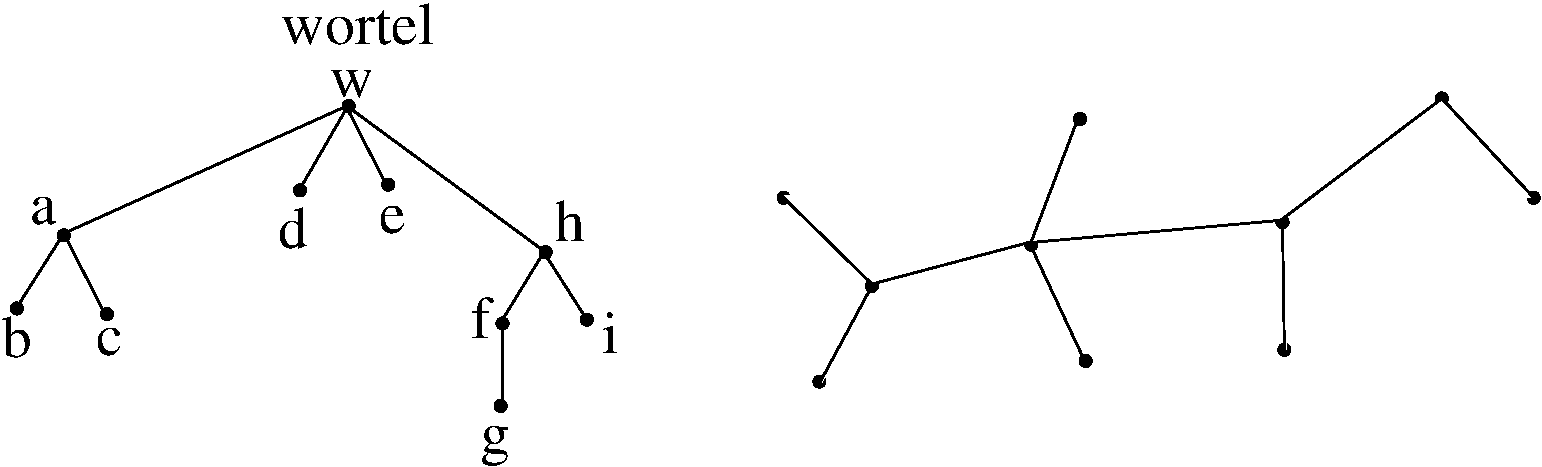
\includegraphics[width=0.5\linewidth,keepaspectratio]{bomen1}
\end{center}
\caption{Examples of trees \label{bomen1}}
\end{figure}


Figure~\ref{bomen1} shows a tree with root $w$ and a tree without a
root. The heights of $a,b,c,d,e,f,g,h,i$ and $w$ are 1,2,2,1,1,2,3,1,2
and 0.

\begin{figure}[ht]
\centering
\mbox{
\subfigure[ Decision tree]{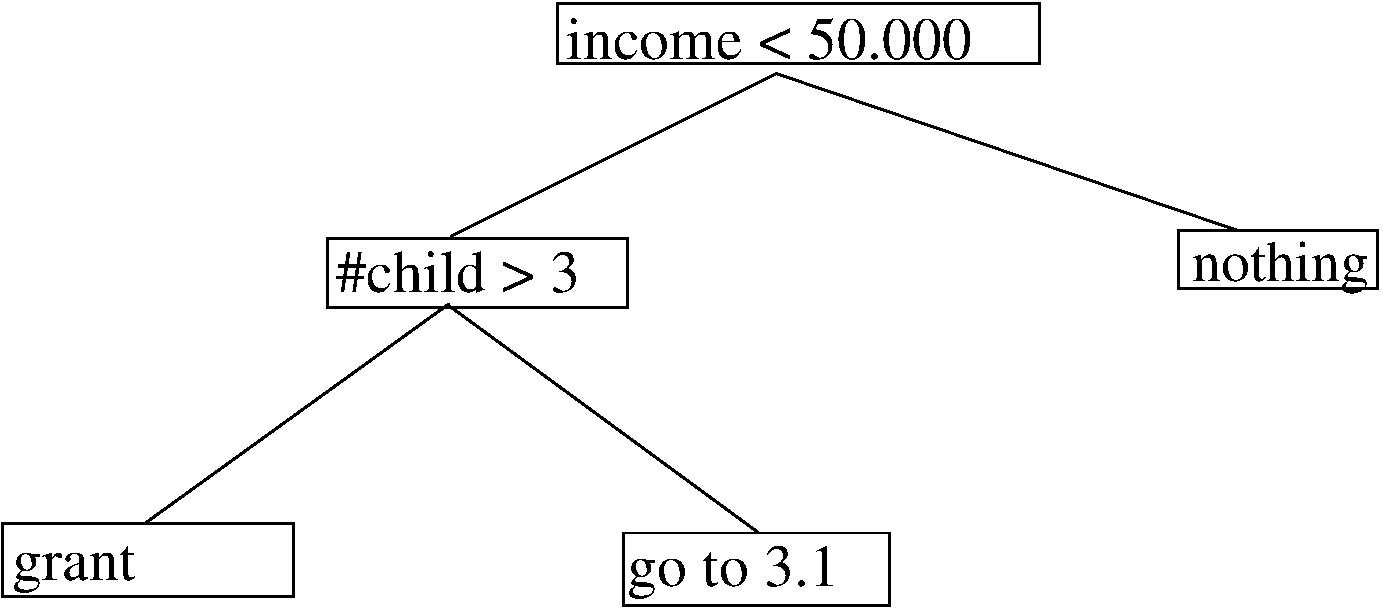
\includegraphics[width=0.5\linewidth,keepaspectratio]{decisiontree1eng} \label{decisiontree1}} %\quad
\subfigure[Representation of $(3+1) *5 - 7/3$]{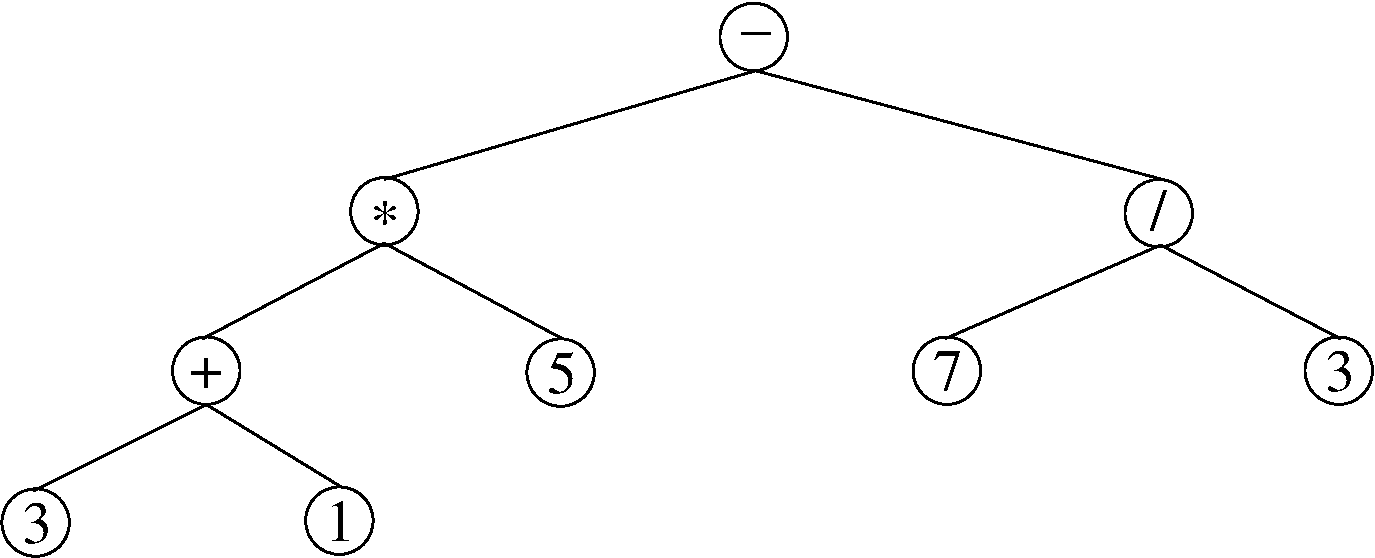
\includegraphics[width=0.5\linewidth,keepaspectratio]{expr1} \label{expr1} }}
\caption{Useful trees}
\end{figure}


Figure~\ref{decisiontree1} shows a decision tree: each vertex
contains a test. The idea is that you start at the root of the tree,
and depending on the answer in the test, you move down left or
right. In this way, you could get advice on whether you are eligible
for financial support.


Figure~\ref{expr1} shows a tree representation of the arithmetic
expression $(3+1) *5 - 7/3$.

%===============================================================================
\section{Properties of Trees}

The following theorem gives 4 equivalent characterisations of trees:

 \begin{theorem}
For a simple graph $T$ with $n$ vertices
 $(a) \Leftrightarrow
  (b) \Leftrightarrow (c) \Leftrightarrow (d)$ with \\[2mm]
(a) $T$ is a tree\\
(b) $T$ is connected and cycle free\\
(c) $T$ is connected and has exactly $(n-1)$ edges\\
(d) $T$ is cycle free and has exactly $(n-1)$ edges
\end{theorem}
\begin{proof} We prove that $(a) \Rightarrow (b)$, $(b) \Rightarrow
(c)$, $(c) \Rightarrow (d)$ and $(d) \Rightarrow (a)$
\begin{itemize}
\item $(a) \Rightarrow (b)$: since $T$ is a tree, there is a path
between any two vertices, so $T$ is connected; if $T$ contained a
cycle, some vertices would be connected by more than one path, so $T$
is cycle free
\item $(b) \Rightarrow (c)$:
we prove this by induction on $n$ that $T$ has $(n-1)$ edges; for
$n=1$ $T$ has zero edges, so the basis for the induction is true;
suppose that every connected cycle free graph with $n$ vertices has
$(n-1)$ edges; consider a connected cycle free graph $S$ with $(n+1)$
vertices; choose a simple path $P$ of maximal length in $S$
(convince yourself this is possible); $P$ contains a vertex $v$ with
$\delta(v) = 1$, because there are no cycles in $S$: indeed, when
$\delta(v) > 1$ then one can extend $P$; consider $S \setminus v$ -
the graph $S$ from which $v$ is removed; $S \setminus v$ has $n$
vertices, is cycle free and connected, so by induction $S \setminus v$
has $(n-1)$ edges; consequently, $S$ has $n$ edges

\item $(c) \Rightarrow (d)$: suppose $T$ contains a cycle; we can now
remove at least one edge (and no vertices) from $T$ to obtain a
connected, cycle free graph $T_{*}$; so we can use the previous result
(from $(b) \Rightarrow (c)$, meaning $T_{*}$ has $(n-1)$ edges; this
means that $T$ has strictly more than $(n-1)$ edges, so we get a
contradiction, from which we must conclude that $T$ is cycle free

\item $(d) \Rightarrow (a)$:
we need to prove that $T$ is connected, and that there is a unique
path between every two vertices; consider the partition of $T$ in its
connected components $\{T_{i}\}_{i=1}^{k}$; let the number of vertices
in $T_{i}$ be equal to $n_{i}$; each of the $T_{i}$ is connected and
cycle free, so $T_{i}$ has $(n_{i}-1)$ edges; summing these we get:
$(n-1) = \sum_{i=1}^{k} (n_{i}-1) = \sum_{i=1}^{k} (n_{i}) - k = n - k$;
from this it follows that $k=1$, so $T$ is connected; now suppose that
there exist two different paths from $a$ to $b$: those two paths form
a cycle, but $T$ is cycle free; we conclude that there is a unique
path between every two nodes; so $T$ is a tree

\end{itemize}
\end{proof}

One reason why this theorem is important is this: to walk around in a
general graph is dangerous, because you run the risk to run in circles
(cycles), and your program could easily end up in an infinite loop.
To prevent that, you need to do extra work, for instance keep track of
all the nodes you have visited already. The theorem above tells us
that in a tree, your walk will end if you always go {\em forward},
i.e. never go back to the (one) previous node. The reason is that a
tree has no cycles. So, if you know that you are dealing with trees,
you can and should use that fact in your program.


 \begin{definition}[Terminology related to trees]
\textup{For a tree $T$ with root $v_{0}$, let $x$, $y$ and $z$ be
vertices in $T$ and $(v_{0}, v_{1}, \ldots , v_{n})$ a path.
} {\rm
\begin{verse}
%\begin{itemize}
%\item
\hspace*{1ex}$\bullet$
$v_{n-1}$ is the \textbf{parent} of $v_{n}$; we often say father (or mother)

%\item
\hspace*{1ex}$\bullet$
$v_{0}$ \ldots\ $v_{n-1}$ are all
\textbf{ancestors} of $v_{n}$, and $v_{n}$ is a \textbf{descendant} of
$v_{0}$ \ldots\ $v_{n-1}$
%\item

\hspace*{1ex}$\bullet$
$v_{n}$ is a \textbf{child} of $v_{n-1}$
%\item

\hspace*{1ex}$\bullet$
if $x$ and $y$ have the same parent, then $x$ and $y$ are siblings
%\item

\hspace*{1ex}$\bullet$
if $x$ has no child, $x$ is a \textbf{leaf}, also called {\bf external node}
%\item

\hspace*{1ex}$\bullet$
if $x$ is not a leaf, $x$ is an \textbf{internal node}
%\item

\hspace*{1ex}$\bullet$
a subgraph of $T$ with vertex $x$ and all descendants of $x$, is a
{\bf subtree} of $T$ rooted at $x$\footnotemark
%\end{itemize}
\end{verse}}
\end{definition}
\footnotetext{Actually, you should prove that this subgraph is a tree!}

Relating this to Figure~\ref{boom1}:

\begin{figure}[ht]
\begin{center}
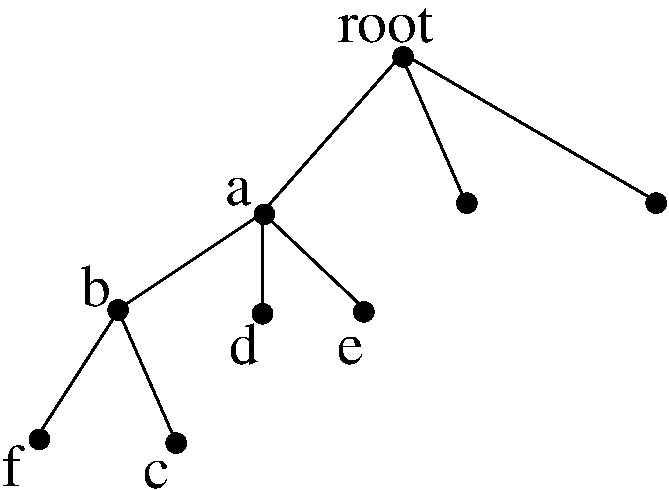
\includegraphics[width=0.25\linewidth,keepaspectratio]{boom1eng}
\end{center}
\caption{Example tree \label{boom1}}
\end{figure}

\begin{itemize}
\item
$c,d,e$ are leaves
\item
$a$ is the parent of $d$
\item
$b,c,f$ are descendants of $a$
\item
$a$ and {\em root} are the ancestors of $b$
\item
$b,d,e$ are siblings
\item
$a,b$ are internal nodes
\item
the subtree rooted in $a$ contains the vertices $a,b,c,d,e,f$
\end{itemize}

Often, the order of the siblings is important, especially with binary
trees.

 \begin{definition}[Binary tree]
\textup{A \textbf{binary tree} is a rooted tree in which every node
has 0, 1, or 2 children; because of the way binary trees are drawn and
used, we speak of a left child (connected to its parent by the left
branch) and a right child (\ldots); this makes an order on the branches
explicit.  }
\end{definition}

You already saw a binary tree in Figure~\ref{decisiontree1}: it is
important to know whether to go left or right on a positive answer to
the test in an internal node.

 \begin{definition}[Full  binary tree]
\textup{A \textbf{full binary tree} is a binary tree
in which every internal node has exactly two children.  }
\end{definition}

\begin{figure}[ht]
\begin{center}
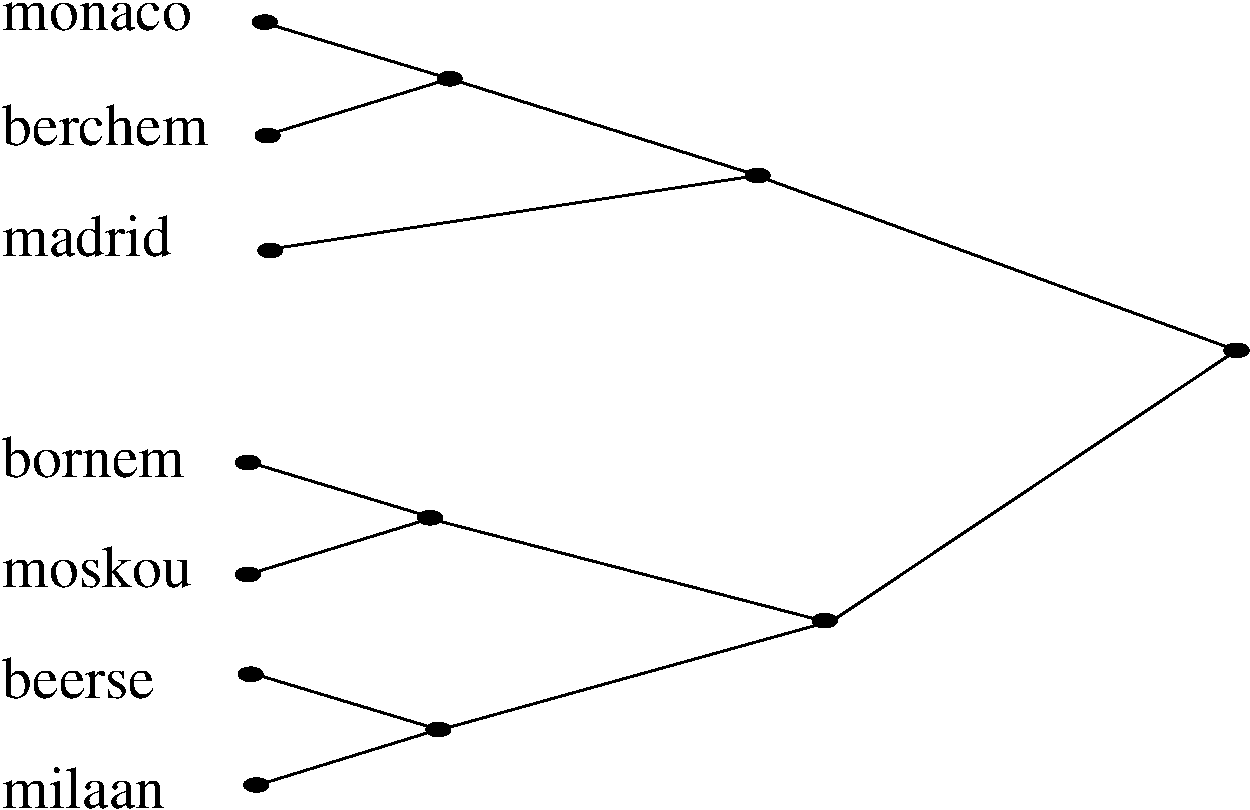
\includegraphics[width=0.5\linewidth,keepaspectratio]{tornooi1}
\end{center}
\caption{Tournament tree \label{tornooi1}}
\end{figure}


Figure~\ref{tornooi1} shows a tournament tree: it is a full binary tree.

 \begin{theorem}
\label{relatiebladinwendig}
A full binary tree $T$ with $i$ internal vertices has
$(i+1)$ leaves and $(2i+1)$ vertices.
\end{theorem}
\begin{proof} Each internal vertex has 2 children, so there are $2i$
children in $T$; there is exactly one vertex that is not a child: the
root; so there are $2i+1$ vertices. Each vertex is either a leaf or
internal, so the number of leaves equals $2i+1 - i = i+1$
\end{proof}


In a tournament with $n$ participants, and direct elimination, you
could wonder how many matches must be played before the winner is
known. Since the tournament tree has $n$ leaves, the number of
internal nodes is $n-1$, and that is the number of matches.

 \begin{theorem}
\label{relatieheightbladeren}
For a binary tree $T$ with height $h$ and $t$ leaves $\log_2(t) \leq
h$ (or $t \leq 2^h$).
\end{theorem}
\begin{proof}
We prove the theorem by induction on $h$ and by considering the
subtrees of $T$: for $h=0$, there is one leaf (the root), so
$t=1=2^h=2^0$ this provides the base case.

Assume $h > 0$; consider $T_{l}$ and $T_{r}$, the left and right
subtree of the root of $T$. $T_{l}$ or $T_{r}$ can be empty, but not both.
Assume $T_{r}$ is empty: then we have $h_{l} = h-1$, and by induction
$t_{l} \leq 2^{h_{l}}$; since $t_{l} = t$ we get $t \leq 2^{h-1}\leq
2^h$.

If $T_{l}$ is empty, we can reason analogously.

Suppose neither $T_{l}$ nor $T_{r}$ is empty; so $h_{l} \leq h-1$ and
by induction $t_{l} \leq 2^{h_{l}}$ and similarly $t_{r} \leq
2^{h_{r}}$, so $t=t_{l} + t_{r} \leq 2^{h_{l}} + 2^{h_{r}}\leq
2^{h-1}+2^{h-1}=2^h$.
\end{proof}

 \begin{theorem} For a binary tree $T$ with $n$ vertices and
height $h$ $\log_2(n+1) \leq h+1$
\label{relatieheightnodes}
\end{theorem}
\begin{proof}
Extend the tree $T$ to a tree $T'$ as follows:
\begin{itemize}
\item
add a left and right branch to every leaf
\item
add a left branch to each internal node missing a left branch
\item
add a right branch to each internal node missing a right branch
\end{itemize}

$T'$ has $n$ internal vertices (all the vertices of $T$) and height
$(h+1)$; $T'$ is full and binary, so we can apply
Theorem~\ref{relatiebladinwendig} and conclude that $T'$ has
$(n+1)$ leaves, and by Theorem~\ref{relatieheightbladeren} $\log_2(n+1)
\leq h+1$.
\end{proof}

Figure~\ref{uitbreiding1} shows a tree and its extension as defined in
Theorem~\ref{relatieheightnodes}: the added vertices are drawn by a
black rectangle. Note that if the original tree is already full, its
extension is different from the original.

\begin{figure}[ht]
\begin{center}
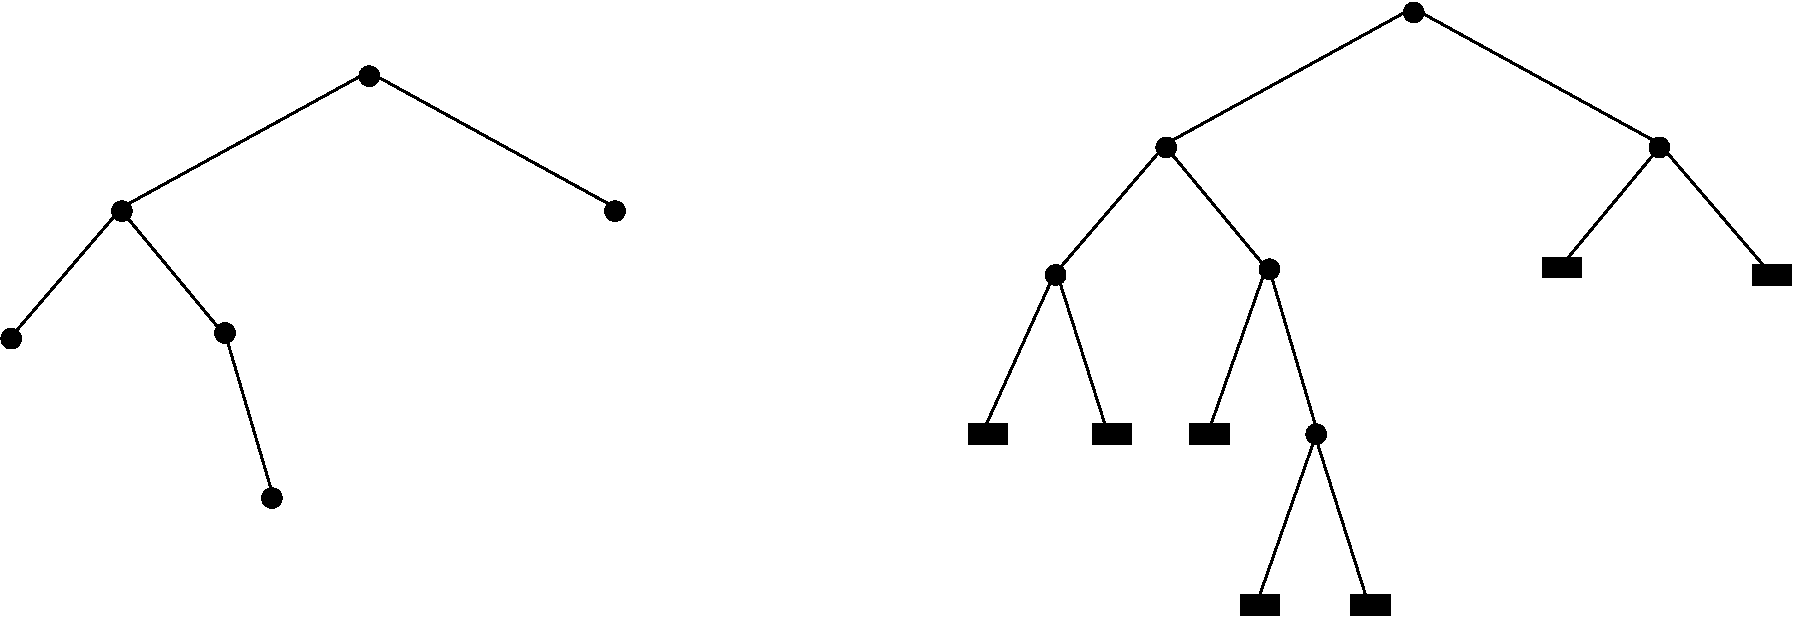
\includegraphics[width=0.6\linewidth,keepaspectratio]{uitbreiding1}
\end{center}
\caption{A binary tree and its extension to a full binary tree\label{uitbreiding1}}
\end{figure}

 \begin{definition}[Binary search tree]
\textup{A \textbf{binary search tree} is a binary tree in which every
vertex $v$ has a value $w(v)$ (e.g. a number or a string) so that
if $l$ belongs to the left subtree of $v$ and $r$ to the right subtree
of $v$, then  $w(l) < w(v) < w(r)$ }
\end{definition}


A binary search tree is also named a sorted binary tree.

Figure~\ref{binboom1} shows a binary search tree in which the values
of the vertices are words; the order is alphabetic.

\begin{figure}[ht]
\begin{center}
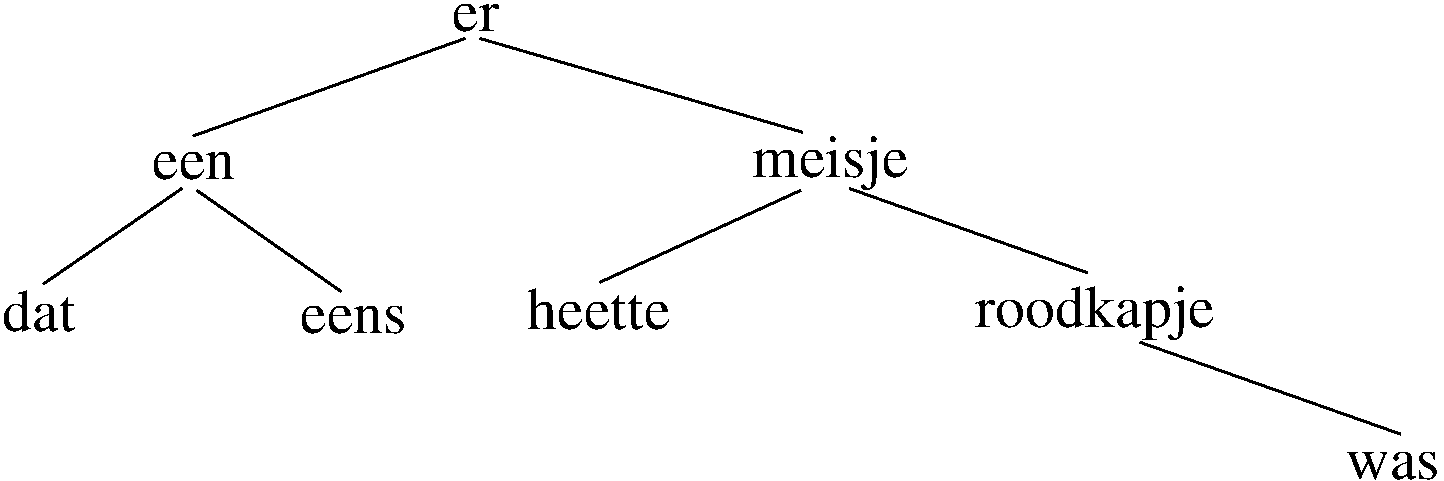
\includegraphics[width=0.6\linewidth,keepaspectratio]{binboom1}
\end{center}
\caption{A binary search tree for the words from the sentence
{\em Er was eens een meisje dat Roodkapje heette} \label{binboom1}}
\end{figure}

The next algorithm searches a given value in a binary search tree: the
algorithm is written as a procedure returning TRUE if the value is
found, and FALSE otherwise.


\parbox{9cm}{
\begin{tabbing}
123456789 \= 12 \= 12 \= 12 \= 12 \= 12 \= 12 \kill
\> boolean search(tree T, value W);\\
\> \{\\
\> \> P = root(T);\\
\> \> while (! empty(P))\\
\> \> \{\\
\> \> \> if (value(P) == W)\\
\> \> \> \> \> return(TRUE);\\
\> \> \> else\\
\> \> \> if (value(P) $<$ W)\\
\> \> \> \> P = rightchild(P);\\
\> \> \> else P = leftchild(P);\\
\> \> \}\\
\> \> return(FALSE);\\
\> \}
\end{tabbing}
}

The complexity of this algorithm can be expressed in the number of
times the body of the while-loop is executed. In the worst case,
the value is not in the tree, and we search along the longest path
starting at the root: that path has length equal to the height $h$ of
the tree, so the loop is executed $h+1$ times. From
Theorem~\ref{relatieheightnodes} we know that $lg(n+1) \leq h+1$, so
for fixed $n$, the worst case is not less than $lg(n+1)$. By balancing
the tree as well as possible, we can achieve $\lceil \log_2(n+1)
\rceil$. Figure~\ref{balanced1} shows two binary search trees with the
same values: the one at the right is balanced better than the one on
the left, and has a smaller height.

\begin{figure}[ht]
\begin{center}
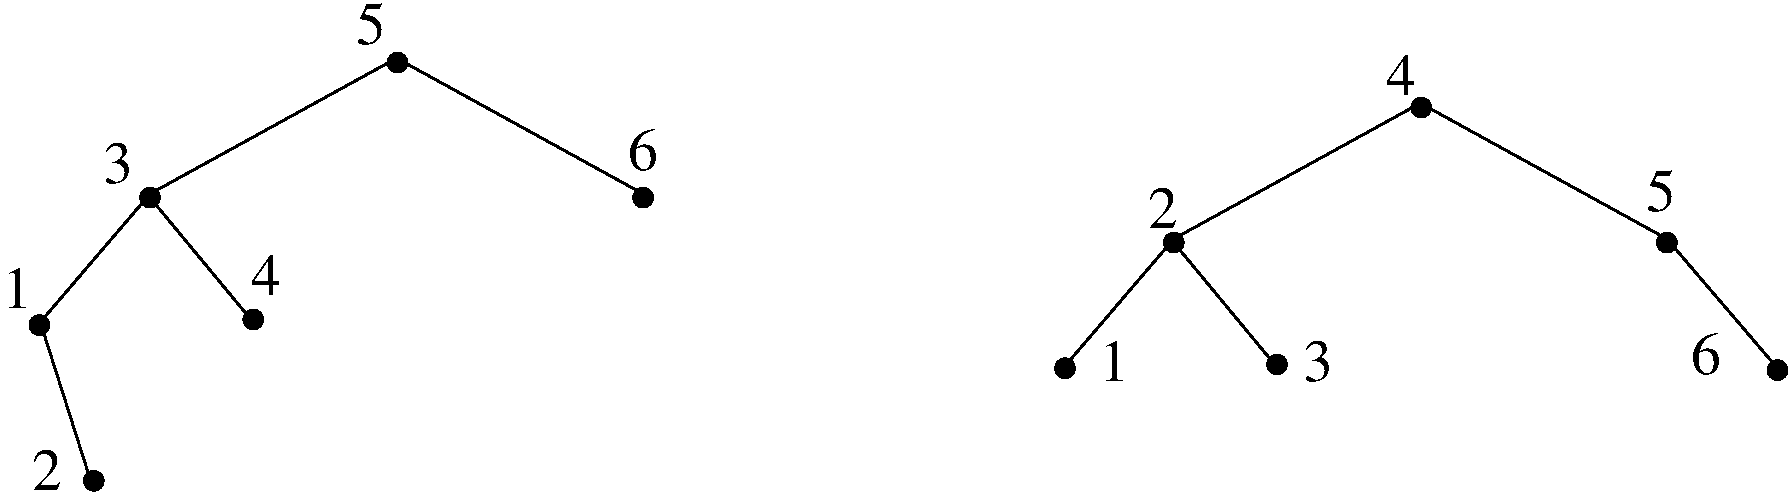
\includegraphics[width=0.6\linewidth,keepaspectratio]{balanced1}
\end{center}
\caption{Two trees with the same values and different height \label{balanced1}}
\end{figure}


%===============================================================================
\section{A Compact Representation}

A tree is often represented with {\em directed} edges. This
representation stresses the fact that often the two functions {\em
leftchild} and {\em rightchild} are explicitly available for use in a
program, but not the function {\em parent}.

It can also be useful to represent a tree as a digraph without cycles
that is not necessarily a tree. As an example take the tree
representation of the expression $(i+7)^{2} + i + 7$ in
Figure~\ref{boomexpressie}. Two subtrees are equal, namely for the
subexpression $i+7$ that occurs twice. The corresponding more compact
representation as digraph can be seen in Figure~\ref{graafexpressie}:
the representation of $i+7$ is now shared.

\begin{figure}[ht]
\mbox{
\hspace{0.5cm}
\subfigure[Tree representation]{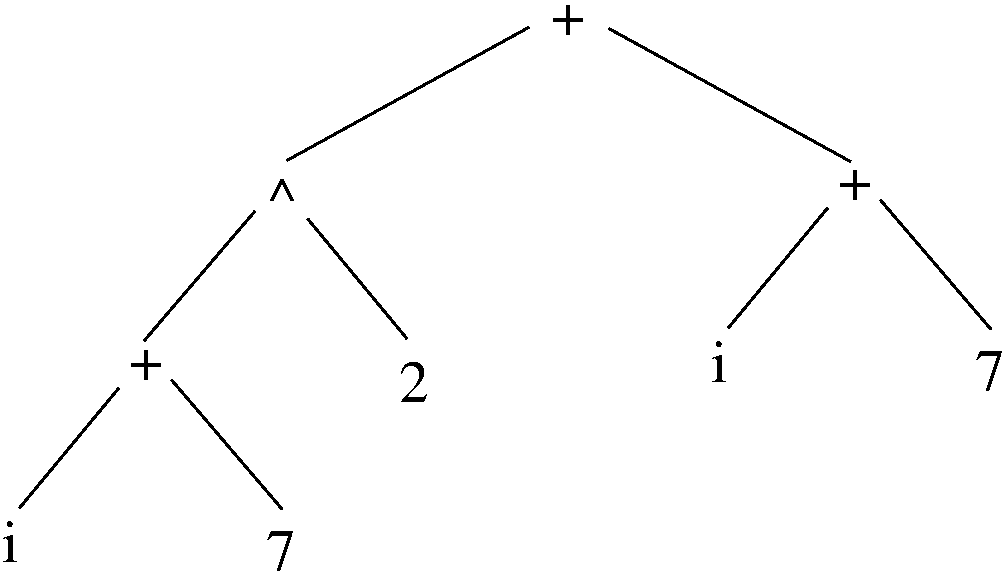
\includegraphics[width=0.4\linewidth,keepaspectratio]{boomexpressie} \label{boomexpressie}}\hspace{1cm}
\subfigure[Graph representation with sharing]{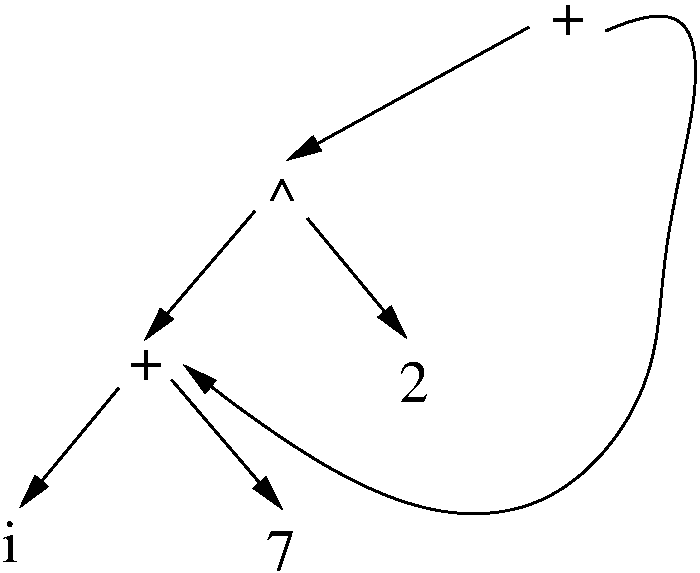
\includegraphics[width=0.3\linewidth,keepaspectratio]{grafeexpressie} \label{graafexpressie} }
}
\caption{Two representations of $(i+7)^{2} + i + 7$}
\end{figure}

Sharing subtrees has its dangers: when the shared subtree is changed,
{\em both} occurrences change. If that is not intended, one should not
use the more compact representation.

%===============================================================================
\section{Spanning Trees}

In this section, we only consider simple graphs: convince yourself
(later) that this is not a severe restriction.

 \begin{definition}[Spanning tree]
A tree \textup{$T$ is a \textbf{spanning tree} of a graph $G$,
if it is a subgraph of $G$ containing all vertices of $G$.}
\end{definition}

A spanning tree covers all vertices of a graph, and it is the smallest
connected subgraph doing so: if you take away an edge from a spanning
tree, you end up with a subgraph that is not a tree.

 \begin{theorem}
A graph $G$ has a spanning tree $T$ if and only if $G$ is connected.
\end{theorem}
\begin{proof}
\begin{itemize}
\item
If $G$ has a spanning tree $T$, then $G$ is connected: a path between
any two edges can use the edges of $T$.

\item
If $G$ is connected and cycle free, then $G$ is a tree and a spanning
tree of itself.

If $G$ is connected and has a cycle, remove one edge from that cycle
(but not the vertices); the resulting graph is still connected and has
one cycle less than $G$; the theorem is now proved by induction on the
number of cycles.
\end{itemize}
\end{proof}

The above theorem does more than prove the existence of a spanning
tree: it gives a constructive method (and algorithm) for finding a
spanning tree: remove an edge from every cycle and you end up with a
spanning tree. An algorithm based on this method is not very
efficient, because we must find cycles and it might be possible to do
better.

\begin{theorem}[Characterisation of spanning tree]\label{opspannend4}
A cycle free subgraph $T$ of a connected graph $G$ that contains a
maximal number of edges of $G$, is a spanning tree of $G$.
\end{theorem}
\begin{proof}

Assume that $G$ has at least 2 vertices.

The fact that $T$ contains a maximal number of edges, means that
that one can't add an edge without introducing a cycle.

We must prove two things: (1) $T$ is connected (which makes it into a
tree); (2) $T$ covers all vertices (making it spanning).


(2) Suppose there exists a vertex $v \in G \backslash T$; since $G$ is
connected, there exits an edge $b$ arriving in $v$; $b \notin T$,
since otherwise $v \in T$; since $T$ is maximal, the graph $T \cup
\{b\}$ contains a cycle that contains $b$. But this means that $v \in
T$, which contradicts the assumption. So $T$ contains all vertices of
$G$.

(1) Suppose that $T$ is not connected; consider the partition of its
components $\{T_{i}\}_{i=1}^{n}$. Figure~\ref{opspannend3} shows
$T_{1}$ and $T_{2}$. Since $G$ itself is connected, there exist
vertices $v_{1} \in T_{1}$ and $v_{2} \in T_{2}$ connected by a simple
path $P$ in $G$ and this path has no other vertices in $T_{1}$ neither
$T_{2}$ (see the dotted line in Figure~\ref{opspannend3}). Suppose $P$
has only one edge $b$. Then $T \cup \{b\}$ contains a cycle through
$v_{1}$ and $v_{2}$; but that means there exists already a path from
$v_{1}$ to $v_{2}$ in $T$, which contradicts the assumption that
$T_{1}$ and $T_{2}$ are two different components.

We still need to prove that in a partition $\{V_{k}\}_{k=1}^{n}$
vertices of a connected graph $G$, there exist always a $V_{i}$ and
$V_{j}$ so that there exist $v_{i} \in V_{i}$, $v_{j} \in V_{j}$, and
an edge $(v_{i},v_{j}) \in G$: consider $V_{1}$ and any other $V_{k}$;
because $G$ is connected, there is a path from a vertex $v_{1} \in
V_{1}$ to a vertex of $V_{k}$; we can choose $v_{1}$ so that the first
edge arrives in a vertex $v \notin V_{1}$. If $v \in V_{k}$, then we
are done. If not, $v$ belongs to another $V_{j}$ and with $j \neq 1$.
\end{proof}


Here is an additional characterisation of spanning trees:

\begin{eig}
A subgraph of a simple connected graph $G$ with $n$ vertices is a
spanning tree of $G$ if $T$ is cycle free and has $n-1$ edges.
\end{eig}

\begin{figure}[ht]
\begin{center}
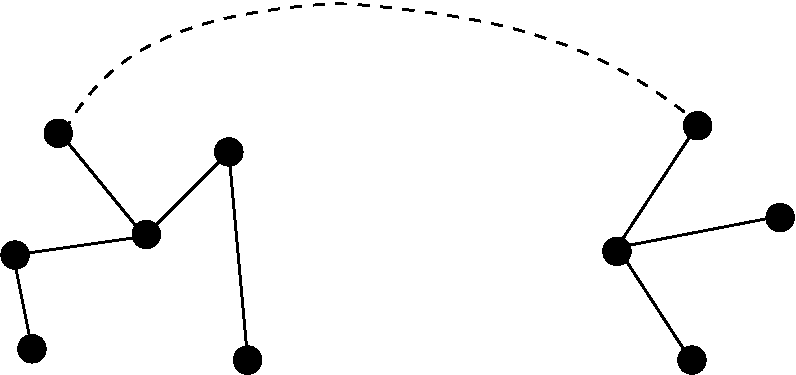
\includegraphics[width=0.3\linewidth,keepaspectratio]{opspannend3}
\end{center}
\caption{Two components of $T$ connected by a path in $G$
\label{opspannend3}}
\end{figure}

Theorem~\ref{opspannend4} leads to a general (non-deterministic)
algorithm for constructing a spanning tree for a graph $G$: start with
the empty tree $T$; repeatedly add an edge to $T$ so that no cycle is
introduced, until this is no longer possible: $T$ is now a spanning
tree.

Note that (1) each edge needs to be considered only once (why?); (2)
the order in which the edges are considered does not matter; (3)
eventually $T$ is a tree, but at intermediate stages, $T$ does not
need to be connected: it is a forest; (4) one can stop trying to add
edges as soon as $T$ has $n-1$ edges.

Two orders for choosing edges are related to general strategies for
tree traversal: {\em depth-first} and {\em breadth-first}. They are
described informally here:

\begin{description}
\item[Depth-first construction of a spanning tree:] choose a vertex
and a construct a simple path starting at this vertex with maximal
length: this path belongs to the spanning tree; back up one step along
that path and start at that node constructing a maximal simple path;
repeat backing up and constructing paths ... until you are back at the
initial vertex and can't construct a path anymore;
Figure~\ref{diepteeerst1} illustrates the method starting from the top
vertex: the solid edges belong to the spanning tree.
\begin{figure}[ht]
\begin{center}
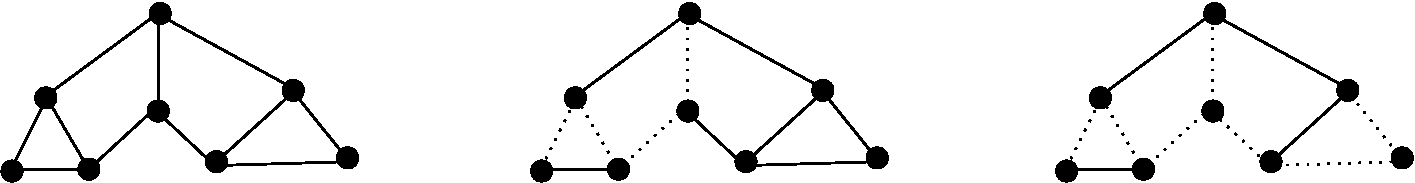
\includegraphics[width=0.6\linewidth,keepaspectratio]{diepteeerst1}
\end{center}
\caption{3 phases in the depth-first construction of a spanning
tree \label{diepteeerst1}}
\end{figure}

\item[Breadth-first construction of a spanning tree:]
choose a vertex and add all edges starting at this vertex make sure no
cycle is made: these edges belong to the spanning tree; repeat this
for all new vertices and keep repeating until no more edge can be
added; Figure~\ref{breedteeerst1} illustrates the method starting from
the top vertex.


\begin{figure}[ht]
\begin{center}
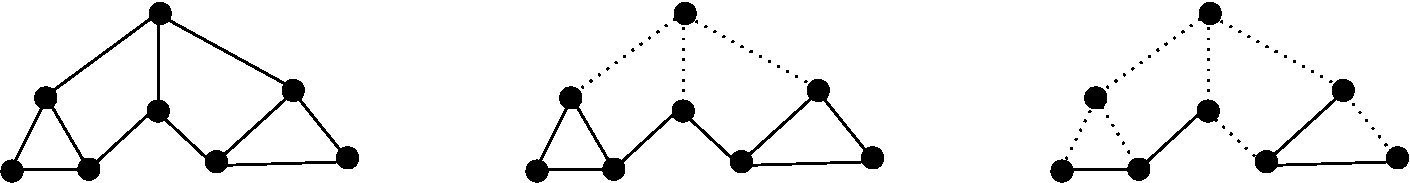
\includegraphics[width=0.6\linewidth,keepaspectratio]{breedteeerst1}
\end{center}
\caption{3 phases in the breadth-first construction of a spanning tree \label{breedteeerst1}}
\end{figure}
\end{description}

The correctness of both methods results from the fact that all edges
are eventually considered for adding to the growing tree, and from
Theorem \ref{opspannend4}. In both methods, the intermediate graph is
a tree, because it is connected and cycle free.

Figure~\ref{opspannend2} shows for $K_{4}$ that depth-first and
breadth-first constructed spanning trees do not need to be isomorphic.

\begin{figure}[ht]
\begin{center}
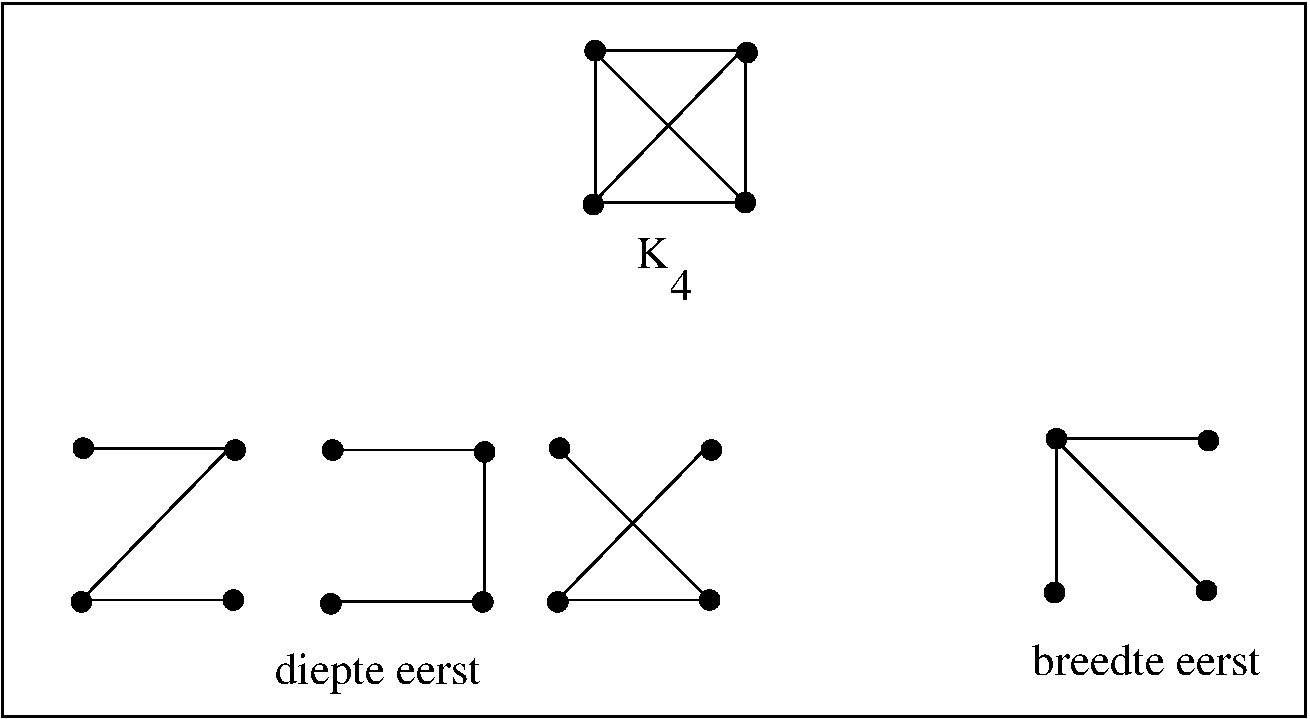
\includegraphics[width=0.5\linewidth,keepaspectratio]{opspannend2}
\end{center}
\caption{Spanning trees for $K_{4}$\label{opspannend2}}
\end{figure}

Maybe you think that {\bf all} spanning trees can be obtained by
either method, but Figure~\ref{opspannend5} shows a graph with a
spanning tree that neither of the methods can compute.

\begin{figure}[ht]
\begin{center}
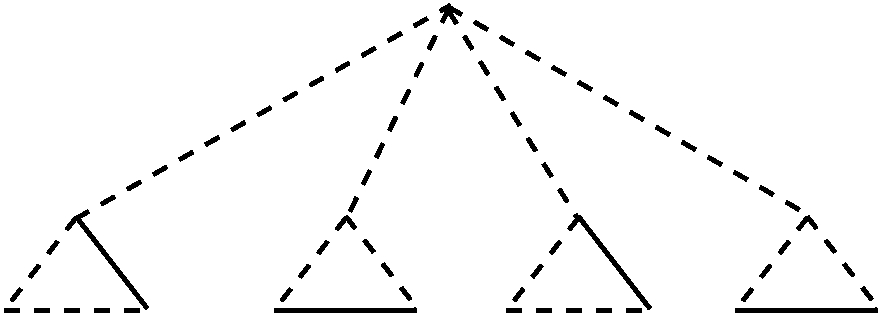
\includegraphics[width=0.5\linewidth,keepaspectratio]{opspannend5}
\end{center}
\caption{Graph with a hybrid spanning tree\label{opspannend5}}
\end{figure}

%===============================================================================
\section{Minimal Spanning Trees}

Consider the following problem: there are a number of cities between
which a road network must be built. The cost of building any road
between two cities is known (it is always strictly positive). We want
to choose which cities to connect by a road, while satisfying two
criteria: (1) the total cost must be minimal, (2) each city must be
reachable from any other city.

Clearly, the network has to be a tree because it can't have cycles
(otherwise the cost would not be minimal), and it must be connected.
This kind of trees is defined as:

 \begin{definition}[Minimal spanning tree (MST)]
\textup{$T$ is a \textbf{minimal spanning tree} of a weighted graph
$G$ if $T$ is a spanning tree of $G$ with minimal weight.}
\end{definition}

Figure~\ref{opspannend1} shows a graph, one of its spanning trees, and
its minimal spanning tree.

\begin{figure}[ht]
\begin{center}
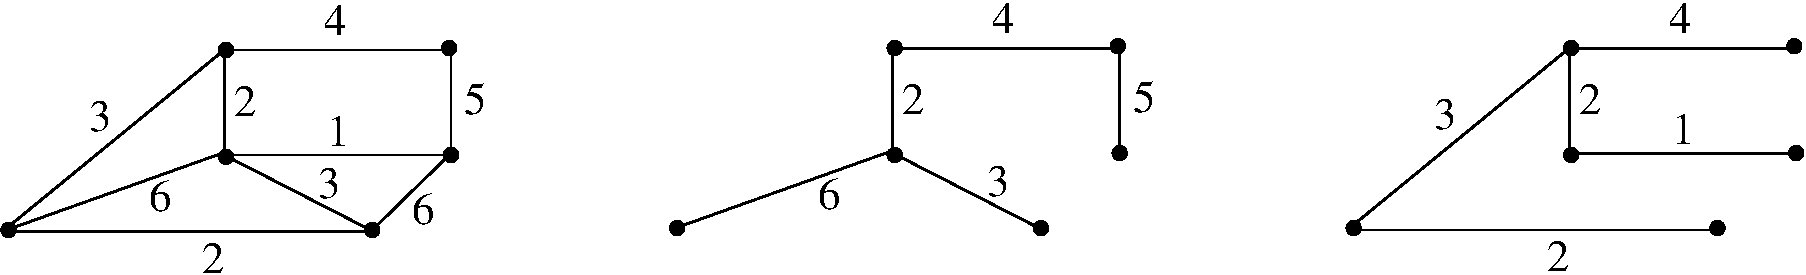
\includegraphics[width=0.6\linewidth,keepaspectratio]{opspannend1}
\end{center}
\caption{A graph with spanning trees\label{opspannend1}}
\end{figure}

Can a graph have more than one MST? Does a graph always have at least
one MST?

Efficient algorithms for constructing an MST are based on the following
theorem:

\begin{theorem} An edge that belongs to an MST \label{even}

Let $(V,E)$ be a connected graph, $U \subset V$ and $e \in E$
so that $e$ has minimal length of all edges between $U$ and $V
\backslash U$. Then $e$ belongs to some minimal spanning tree $T$ of
$(V,E)$.
\end{theorem} % stelling 2.3 from Shimon Even
\begin{proof} Let $T_{0}$ be any MST of $(V,E)$. If $e \in T_{0}$,
then we are done. If not, add $e$ to $T_{0}$, resulting in $T_{1}$
which contains a cycle (Theorem~\ref{opspannend4}). This cycle
contains $e$ and also another edge $e' = (u,v)$ so that $u \in U$ and
$v \in V \backslash U$. Removing $e'$ from $T_{1}$ results in a
spanning tree $T$ (why is $T$ a tree?) and moreover $w(T) \leq
w(T_{0})$ since $w(e) \leq w(e')$. So, $T$ is a minimal spanning tree
containing $e$.
\end{proof}


\begin{code}Prim\label{prim} \\
  Let $G(V,E)$ be a connected weighted graph $G(V,E)$ where the
vertices are numbered: $V = \{v_{1},v_{2},\ldots,v_{n}\}$. The
following procedure constructs a minimal spanning tree $T$ for $G$.
\begin{enumerate}
\item \textbf{Initialisation}: $T := (\{v_{1}\},\emptyset)$
\item \textbf{Stop?}: If $T$ has $(n-1)$ edges, stop.
\item \textbf{Add edge}:
Define $S = \{e | e = (u,v), u \in T, v \notin T\}$ and choose an edge
$b$ from $S$ so that $\forall e \in S: w(b) \leq w(e)$. Add $b$ to
$T$. The result is still connected and cycle free.
Go to \textbf{Stop?}.
\end{enumerate}
\end{code}

\begin{proof}
At the end of the algorithm, $T$ is a tree with $n$ vertices,
$(n-1)$ edges, and cycle free, so $T$ is a spanning tree $G$. We still need to prove termination of the algorithm and the minimality of $T$.

Termination is easy: \textbf{Add edge} is executed $(n-1)$ times, and
then the algorithm stops. Maybe you should convince yourself that
\textbf{Add edge} is always possible as long as $T$ has less than
$n-1$ edges.

Figure \ref{prim2} shows the reasoning below.

After the \textbf{Initialisation}, $T$ consists of one vertex, so at
that moment $T$ is part of an MST. We now prove that this property
is invariant under the application of \textbf{Add edge}:

denote by $W$ the vertices of $T$ and suppose that $T \subset T'$ with
$T'$ an MST. Denote by $B$ the set
%
$\{(x,y)\;|\; x \in W,\; y \in V \backslash W,\; (x,y) \in E\}$.
%
Consider a shortest edge $(i,j)$ in $B$ that does not cause a cycle
when added to $T$. If $(i,j) \in T'$ then clearly $T \cup \{(i,j)\}
\subseteq T' = $ MST. If $(i,j) \notin T'$ then $T' \cup \{(i,j)\}$
contains a cycle which contains $(i,j)$.  This cycle contains another
edge $(x,y) \in B$ and we can take it out of $T' \cup \{(i,j)\}$ so
that we get a new spanning tree $T''$ (it contains all vertices and is
connected and cycle free). So the question is: is $T''$ minimal?
Since $w(i,j) \leq w(x,y)$ (that is how $(i,j)$ was chosen), we
have $w(T'') \leq w(T')$ so $T''$ is an MST. We can conclude that
$T \cup \{(i,j)\}$ is part of an MST.

As a result, the spanning tree constructed by Prim is a minimal
spanning tree.
\end{proof}

\begin{figure}[ht]
\begin{center}
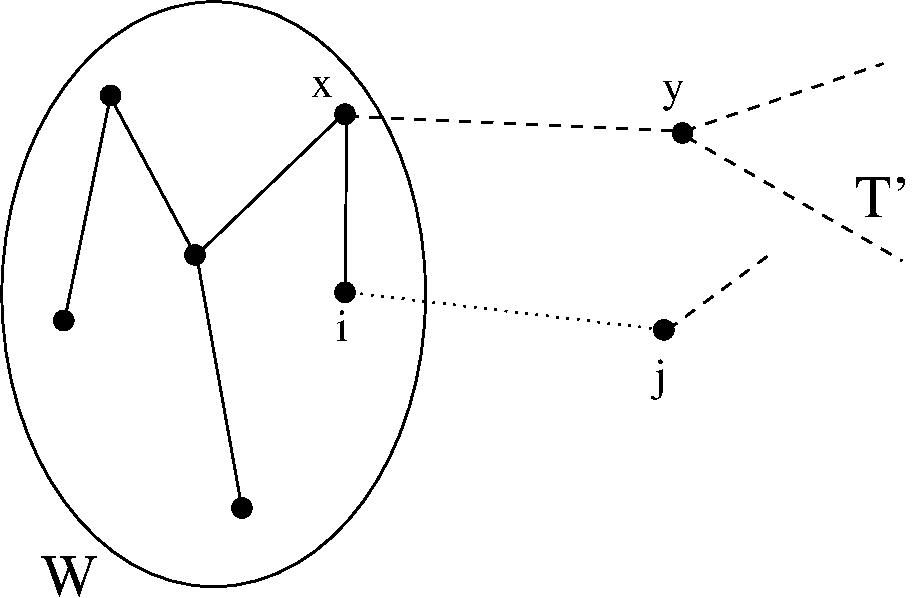
\includegraphics[width=0.4\linewidth,keepaspectratio]{prim2}
\end{center}
\caption{Illustration of the Algorithm~\ref{prim} \label{prim2}}
\end{figure}


Prim's algorithm is a classic example of a {\em greedy} algorithm: any
time a choice needs to be made, the decision is made taking very
little into account, and definitely not the future choices. Exactly
because of Theorem \ref{even}, this greedy algorithm delivers the
optimal solution. That is not true for every greedy algorithm: a
shortest path algorithm that would choose at any junction the shortest
edge leaving that junction, often does not give an overall shortest
path; also, a greedy chess player loses more often than they win.

Prim's algorithm is illustrated in Figure~\ref{prim1}: the initial
vertex is A; the order in which the edges are added, is indicated as
a,b,c \ldots h.

\begin{figure}[ht]
\begin{center}
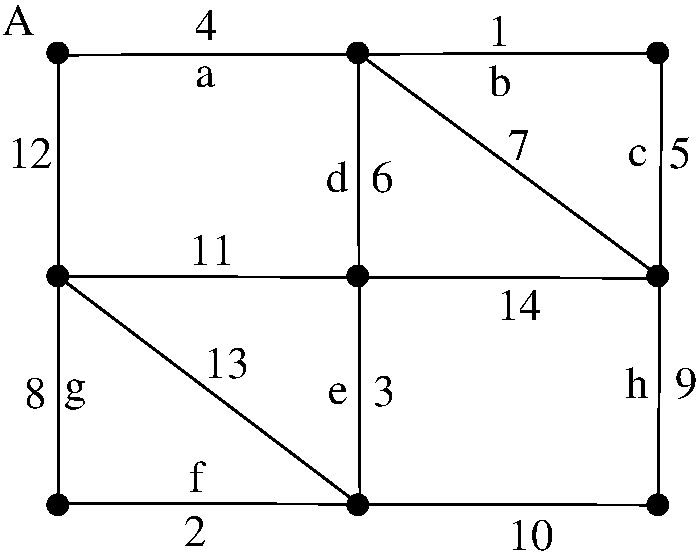
\includegraphics[width=0.3\linewidth,keepaspectratio]{prim1} % ,height=5cm}
\end{center}
\caption{Prim's algorithm~(\ref{prim}) executed \label{prim1}}
\end{figure}


Prim's algorithm builds the MST incrementally: at each moment during
the execution of the algorithm, $T$ is an MST of a subgraph of
$G$. There is also a variant of Prim's algorithm without this
property:


\begin{code} Kruskal \label{kruskal}\\
  Let $G(V,E)$ be a connected weighted graph $G(V,E)$ where the
vertices are numbered: $V = \{v_{1},v_{2},\ldots,v_{n}\}$. The
following procedure constructs a minimal spanning tree $T$ for $G$.
\begin{enumerate}
\item \textbf{Initialisation}: $T := \emptyset$
\item \textbf{Stop?}: If $T$ has $(n-1)$ edges, stop.
\item \textbf{Add edge}: Add to $T$ an edge $b$ with minimal weight
  that does not introduce a cycle in the result. Go to {\bf Stop?}.
\end{enumerate}
\end{code}
\begin{proof}
Termination of Kruskal is proven as for Prim.

The proof that $T$ is a spanning tree at the end, is also similar.

We prove minimality of $T$. Assume $T$ is not an MST.  Name the edges
of $T$ $b_{1},b_{2},\ldots ,b_{n-1}$ in the order as added by the
algorithm. Let $S$ be an MST of $G$ so that
%
$\{b_{1}, b_{2}, \ldots , b_{i}\} \subseteq S$ and with maximal $i$
(such an $S$ exists and by Theorem~\ref{even} $i \geq 1$!). There are
now two possibilities:
\begin{itemize}
\item
\textbf{$i = n-1$}: this means that $T = S$ so $T$ is an MST.
\item
\textbf{$i < n-1$}: now $b_{i+1} \notin S$; let $H$ be the graph with
the edges $\{b_{1}, b_{2}, \ldots , b_{i}\}$ (and their
vertices). Consider the graph $S \cup \{b_{i+1}\} = S'$. $S'$ has a
cycle with at least one edge $b$ not belonging to $T$ (because $T$ is
itself cycle free). So, $b \in S$. $H \cup \{b\}$ is cycle free,
because $H \cup \{b\} \subseteq S$ and since Kruskal added edge
$b_{i+1}$ in the $(i+1)^{th}$ \textbf{Add edge} (for addition to $H$),
we know that $w(b_{i+1}) \leq w(b)$. Consequently $S' \backslash \{b\}
= S''$ is an MST. But that makes $S''$ into an MST that contains
$\{b_{1}, b_{2}, \ldots , b_{i+1}\}$, in contradiction with the
maximality of $S$. It follows that $i < n-1$ is not possible.
\end{itemize}
\end{proof}

Note that during Kruskal, $T$ does not need to be a tree all the
time. The execution of Kruskal's algorithm is illustrated in
Figure~\ref{kruskal1} on the same graph as in Figure~\ref{prim1}.

\begin{figure}[ht]
\begin{center}
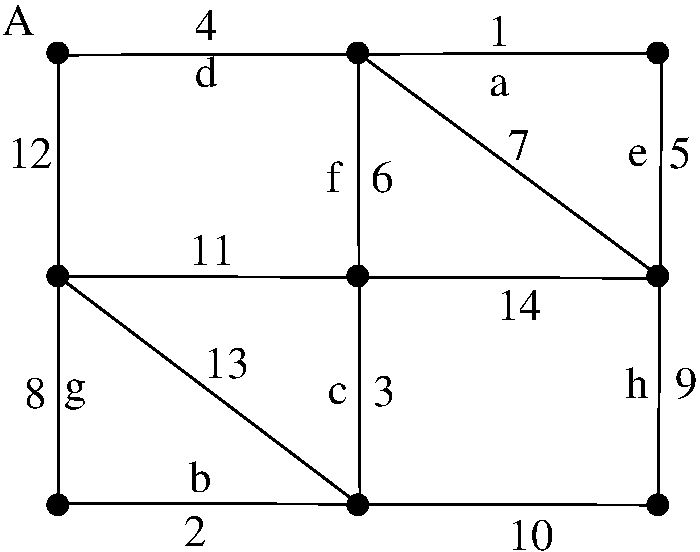
\includegraphics[width=0.3\linewidth,keepaspectratio]{kruskal1} % ,height=5cm}
\end{center}
\caption{Kruskal's algorithm executed}\label{kruskal1}
\end{figure}


%///////////////////////////////////////////////////////////////////////////////
\chapter{Network Models}

A network of connections with each having its own capacity can be modelled by
a directed, weighted graph. The following are examples of such
networks: a road network, an electrical network, oil pipes \ldots An
interesting and important problem in this area is the optimization
of the flow, while respecting the capacities. We will solve this
optimization problem with some graph theory. Problems that are
seemingly unrelated to flow optimization can often be modelled as a
network problem as well: personnel assignment, resource allocation and
even partner choice - the latter is known as the {\em marriage
  problem}.


%===============================================================================
\section{Transport Networks}

 \begin{definition}[Transport network] {\rm A \textbf{transport
         network} (or simply \textbf{network}) is a simple, weighted,
       directed graph $G$ with the following properties:
\begin{verse}
1. there is exactly one vertex in $G$ without incoming edges; this
vertex is called the \textbf{source}

2. there is exactly one vertex in $G$ without outgoing edges; this
vertex is called the \textbf{sink}

3.
the weight $C_{i,j}$ of the (directed) edge $(i,j)$ is positive and is
named the \textbf{capacity} of the edge

4.
disregarding the direction of the edges, $G$ is connected
\end{verse}
}
\end{definition}



Figure~\ref{transport1} shows a network: the source is vertex $a$ and
the sink is $z$; the capacity of an edge is written next to the
edge. The network could model a number of one way streets in a city
with a railway station $a$ and a market place $z$; the capacity could
be the number of vehicles that can pass through the street per minute.

\begin{figure}[ht]
\begin{center}
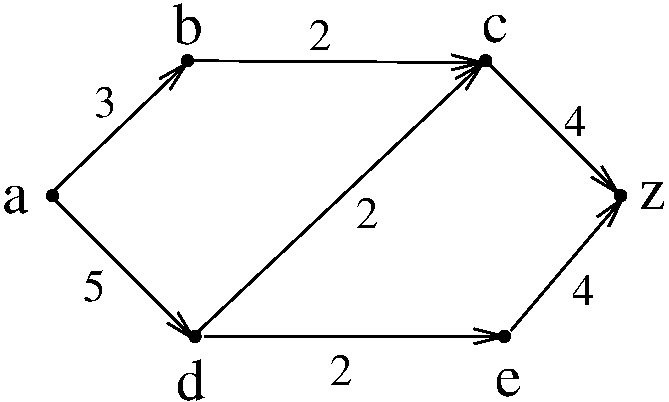
\includegraphics[width=0.3\linewidth,keepaspectratio]{transport1} % ,height=3cm}
\end{center}
\caption{A transport network \label{transport1}}
\end{figure}

The restriction to simple graphs is not so bad: loops and parallel
edges can be simply removed by putting an extra vertex on such
edges. This changes nothing essential as far as the problems studied
later in this section are concerned.


\begin{definition}[Network flow]\label{stroming1}
\label{stromingdef}
{\rm A {\bf network flow} $F$ in a network $G(V,E)$ with capacities
  $C_{i,j},\;\; i,j \in V$\footnotemark is a mapping from $E$ to
  $\R^{+}$ so that\\
\begin{minipage}{12cm}
\begin{enumerate}
\item
\label{stromingdef1}
$F(i,j) \leq C_{i,j}$
\item \label{conserve1} for each vertex $j$ different from source and
  sink:
\[\displaystyle \sum_{i \in V} F(i,j) = \sum_{i \in V} F(j,i)\]
\end{enumerate}
\end{minipage}\\[2mm]
We name $F(i,j)$ the flow in edge $(i,j)$. For a vertex $j$, we name
the quantity $\sum_{i \in V} F(i,j)$ the incoming flow in $j$, and
$\sum_{i \in V} F(j,i)$ the outgoing flow out of $j$.  }
\end{definition}
\footnotetext{if there is no edge $(i,j)$, we assume that $C_{i,j} = 0$}



Formula~\ref{conserve1} in Definition~\ref{stroming1} expresses the
law of conservation of goods: everything that comes into an edge must
get out as well. That prevents accumulation of goods in a vertex, and
production of goods in a vertex. Think of Kirchhoff's law.

Figure~\ref{stroom2} shows a flow for the network of Figure
\ref{transport1}; the flow is defined by:
\begin{center}
$
\begin{array}{l}
F(a,b) = 2\\
F(b,c) = 2\\
F(c,z) = 3\\
F(a,d) = 3\\
F(d,c) = 1\\
F(d,e) = 2\\
F(e,z) = 2\\
\end{array}
$
\end{center}
It is marked next to the capacity of the corresponding edge.
\begin{figure}[ht]
\begin{center}
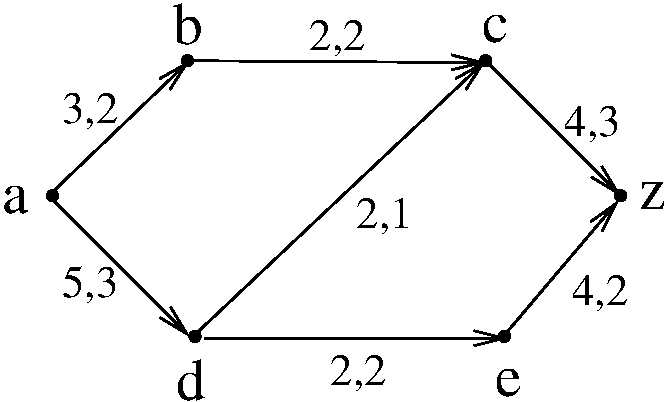
\includegraphics[width=0.3\linewidth,keepaspectratio]{stroom2} % ,height=3cm}
\end{center}
\caption{A transport network flow \label{stroom2}}
\end{figure}

You can check that Formula~\ref{conserve1} in
Definition~\ref{stroming1} is satisfied for each vertex, except the
source and the sink.

You can also check that the flow coming out of the source equals the
flow coming into the sink.

\begin{center}
\mbox{$F(a,b)+F(a,d) = F(c,z) + F(e,z)$}.
\end{center}
This equality is more generally true:

 \begin{theorem}[Source-out = sink-in \label{source=sink}]
For any flow $F$ in a network $G(V,E)$, the flow coming out of the
source equals the flow going into the sink, or more formally:
\[\sum_{i \in V} F(a,i) = \sum_{i \in V} F(i,z).\]
\end{theorem}
\begin{proof}

It should be clear that

$~~~~~~~~~~\sum_{j \in V} (\sum_{i \in V} F(i,j))  =
                \sum_{i \in V} (\sum_{j \in V} F(i,j))
         =  \sum_{j \in V} (\sum_{i \in V} F(j,i))$

Interchanging the $\sum$'s is allowed as we are dealing with finite
graphs. The second equality holds because we only renamed $i$ and $j$.

It follows that

\begin{tabular}{c c c l}
~~~~~~~~~ &
0 & = & $\sum_{j \in V} \left(\sum_{i \in V} F(i,j) - \sum_{i \in V} F(j,i) \right)$\\
 & & & \\
 &  & = & $\left( \sum_{i \in V} F(i,z) -  \sum_{i \in V} F(z,i)\right) +
                \left(\sum_{i \in V} F(i,a) -  \sum_{i \in V} F(a,i)\right)$
    \\
 & & & \\
 &  &  & \hspace*{2cm}
       $+ \sum_{j \in V \backslash \{a,z\}} \left( \sum_{i \in V} F(i,j) -
                \sum_{i \in V} F(j,i)\right)$\\
 & & & \\
 & & = & $\sum_{i \in V} F(i,z) - \sum_{i \in V} F(a,i)$
\end{tabular}



since $F(z,i) = 0 = F(i,a)$ for $\forall i \in V$ (by Definition~\ref{stromingdef})

and  $\sum_{i \in V} F(i,j) = \sum_{i \in V} F(j,i)$  $\forall j \in
(V \backslash \{a,z\})$ (by Formula~\ref{conserve1} in
Definition~\ref{stromingdef})
\end{proof}



Theorem~\ref{source=sink} justifies the following:

 \begin{definition}[Value of a flow]
\textup{The \textbf{value of a flow $F$} in a network $G(V,E)$
with source $a$ and sink $z$ is $\sum_{i \in V} F(a,i)$ or
$\sum_{i \in V} F(i,z)$ }
\end{definition}

The value of the flow in Figure~\ref{stroom2} is 5.



The network problem can now be formulated as: for a given network $G$,
find a maximal flow, i.e. a flow with maximal value.


Before we go into that \ldots Networks could have more than one source
and/or sink: the network in Figure~\ref{transport2} could represent
the water supply of cities $A$ and $B$, from sources $X,Y$ and $Z$,
and with intermediate distribution centers $b,c$ and $d$.

\begin{figure}[ht]
\begin{center}
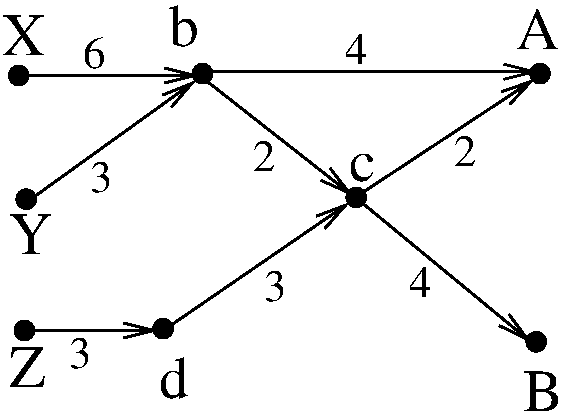
\includegraphics[width=0.22\linewidth,keepaspectratio]{transport2} % ,height=3cm}
\end{center}
\caption{A transport network with more than one source and sink \label{transport2}}
\end{figure}

One can add a super source $a$ and a super sink $z$ to the network, an
edge from $a$ to each original source with infinite capacity, and an
edge from each sink to the super sink, also with infinite capacity: we
get the usual network.

\begin{figure}[ht]
\begin{center}
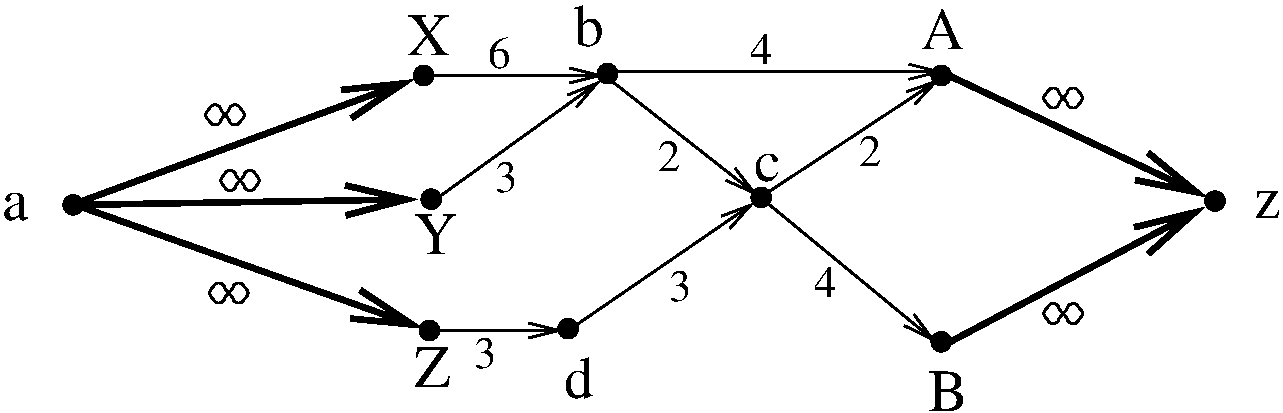
\includegraphics[width=0.507\linewidth,keepaspectratio]{transport3} % ,height=3cm}
\end{center}
\caption{The same transport network with a super source and a
super sink \label{transport3}}
\end{figure}

A maximal flow in the new network corresponds to a maximal flow in the
original network: convince yourself about that.

Finally, a maximal flow is often not unique: Figure~\ref{stroom3}
shows a network with infinitely many maximal flows. Indeed, for each
$i$ and $j$ satisfying $i+j = 5$ and $0 \leq i,j \leq 3$, the flow is
maximal.

\begin{figure}[ht]
\begin{center}
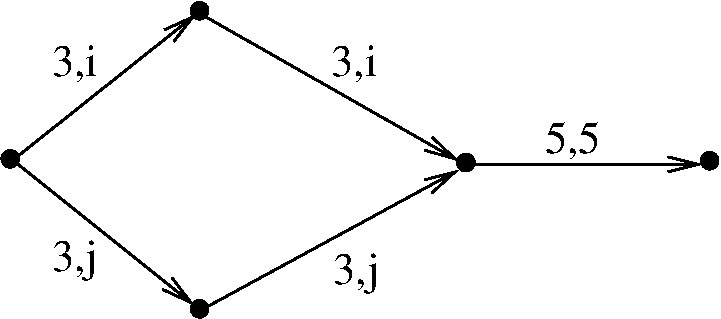
\includegraphics[width=0.3\linewidth,keepaspectratio]{stroom3} % ,height=2.5cm}
\end{center}
\caption{A network with infinitely many maximal flows\label{stroom3}}
\end{figure}


%===============================================================================
\section{Maximal Flow}

The idea behind the next algorithm for computing a maximal flow is as
follows: start from any flow and improve it until no longer possible -
you end up with a maximal flow. The informal description of how to
improve a flow is:
\begin{itemize}
\item
consider a path $P$ from the source $a$ to the sink $z$
\item
find the minimum $\Delta$ of $C_{b} - F(b)$ over all edges $b \in P$
\item
construct the new flow along path $P$ by adding $\Delta$ to each $F(b)$
\end{itemize}

A few remarks about this recipe:
\begin{itemize}
\item the operation increases the flow if and only if $\Delta > 0$
along that chosen path $P$
\item the above only works if all edges in $P$ have the correct (the
{\em good}) direction, but
\item limiting ourselves to paths from $a$ to $z$ along the directed
edges is not enough: look at Figure~\ref{transport4}; no path with
only good edges can be improved with the above method; but the flow
along the path $(a,b,c,z)$ can be improved: the resulting flow is
shown in Figure~\ref{transport5};

\begin{figure}[ht]
\begin{center}
\subfigure[A non-maximal flow]{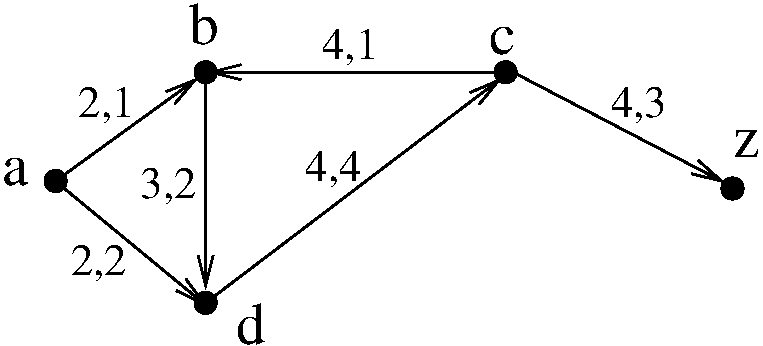
\includegraphics[width=0.3\linewidth,keepaspectratio]{transport4} \label{transport4}}\hspace{1.2cm}
\subfigure[A better flow along a path with a {\em bad}
edge]{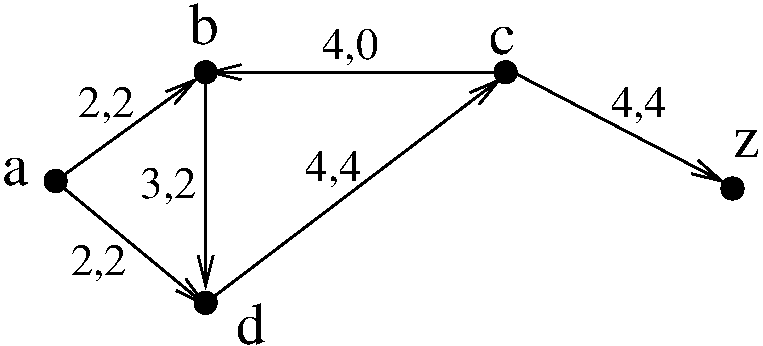
\includegraphics[width=0.3\linewidth,keepaspectratio]{transport5} \label{transport5}}
\end{center}
\caption{Improving a flow}
\end{figure}

It follows that we also need to consider paths with inverted edges,
and we don't add a $\Delta$ to them, we subtract it: if an inverted
edge has a non-zero flow, it is possible that some flow is running in
cycles without ever reaching the sink, while still using up the
capacity of some edges. We formalize this now.

\end{itemize}

 \begin{definition}[Good and bad edges]
\textup{In a digraph $G(V,E)$ with path $(v_{1},v_{2},\ldots ,v_{n})$
we name an edge $(v_{i},v_{i+1})$ \textbf{good} if $(v_{i},v_{i+1})
\in E$, and otherwise \textbf{bad}}
\end{definition}

In a path $P$ , we denote the good edges by $P_{+}$, the bad edges by $P_{-}$.


 \begin{theorem} Improving a flow
\label{verbeterflow}\\
Let $P$ be a path from $a$ to $z$ in a network $G(V,E)$, so that
\begin{verse}
1.
$\forall (i,j) \in P_{+}$: $F(i,j) < C_{i,j}$

2.
$\forall (i,j) \in P_{-}$: $0 < F(i,j)$
\end{verse}

Define $\Delta$ as $min(min_{(i,j) \in P_{+}}
\{C_{i,j}-F(i,j)\},min_{(i,j) \in P_{-}} \{F(i,j)\})$, and the
function $F'$ as:

\begin{eqnarray*}
F'(i,j) & = & F(i,j) \quad \forall (i,j) \notin P\\
        & = & F(i,j) + \Delta \quad \forall (i,j) \in P_{+}\\
        & = & F(i,j) - \Delta \quad \forall (i,j) \in P_{-}
\end{eqnarray*}

Then $F'$ is a flow and it is (strictly) larger than $F$ by $\Delta$.

\end{theorem}
\begin{proof} In order to prove that $F'$ is a flow, we must check
\ref{stromingdef1} and ~\ref{conserve1} from
Definition~\ref{stromingdef}: neither is difficult.

The fact that the flow is improved by $\Delta$, follows from the fact
that the flow over the edge $(a,\_) \in P$ (a good edge! why?) is
increased by $\Delta$, while the flow through the other edges starting
at $a$ has not changed. \end{proof}

One of the consequences of this theorem, is that in a maximal flow $F$
each path from $a$ to $z$ contains at least one good edge with
$C_{i,j} = F(i,j)$ or one bad edge with $F(i,j) = 0$. Otherwise, the
flow can be improved along that path.

We would also like the following properties:

\begin{itemize}
\item
if a flow cannot be improved along any path from $a$ to $z$ (according
to the method of Theorem~\ref{verbeterflow}) then the flow is maximal
- that might look trivial, but remains to be proven!
\item
an algorithm to maximize the flow consists of repeatedly looking for a
path that satisfies the conditions of Theorem \ref{verbeterflow},
and improving the flow over that path, until no more such paths exist;
here we need a systematic way to find relevant paths
\end{itemize}

Both properties will be proven formally. We first describe a classical
algorithm that is actually a {\em labeling procedure}: each vertex
gets a label with information during the execution of the algorithm.
We use a label with two pieces of information: the first component is
{\em the vertex you came from}; the second component is the $\Delta$
from Theorem~\ref{verbeterflow} in the path up to that vertex. The
algorithm makes this more precise.

\begin{code} Construction of a maximal flow.
\label{maxflow}\\
Let $G(V,E)$ be a network with source $a$, sink $z$ and capacity $C$,
and let all the capacities be a positive integer. Define any order on
the vertices: $a = v_{0}, v_{1}, \ldots , v_{n} = z$.

We use ${\cal C}$ to denote the set of considered vertices, ${\cal L}$
for the labeled vertices. We will make the operations on ${\cal C}$
explicit and leave the operations on ${\cal L}$ implicit.

\begin{enumerate} \item \textbf{Initialisation}:
Define $\forall (i,j) \in E: F(i,j) = 0$

\item
\textbf{Label the source}: Give $a$ the label $(\_,\infty)$; set
${\cal C} = \emptyset$

\item
\textbf{Arrived?}: If $z$ has a label, improve the flow and go back to
\textbf{Label the source}.

Improving the flow works as follows: there is exactly one path $P$ from
$a$ to $z$ that can be found by constructing backwards, starting at $z$
and repeatedly following the first component of the label of the
vertex. The second component of the $z$'s label is a quantity $\Delta$
that is added to the flow in the good edges of $P$, and subtracted
from the flow in the bad edges. Finally, erase all labels in the network.

\item
\textbf{Choose the next vertex}: If ${\cal L} \setminus {\cal C} =
\emptyset$, \textbf{stop}: the flow $F$ is maximal.

Let $v$ be the $v_{i} \notin {\cal C}$ with a label and with minimal
index $i$.
\item
\textbf{Label the neighbours}: Suppose the label of $v$ equals
$(\alpha,\Delta)$. Treat any edge of the form $(v,w)$ or $(w,v)$ in
the order $(v,v_{0})$, $(v_{0},v)$, $(v,v_{1})$, $(v_{1},v)$, $\ldots
$ and such that $w$ has no label yet.
\begin{itemize}
\item
for an edge $(v,w)$ (i.e. outgoing of $v$):
if $F(v,w) < C_{v,w}$ than give $w$ the label $(v,min\{\Delta,C_{v,w}-F(v,w)\})$
otherwise, do not label $w$
\item
for an edge $(w,v)$ (i.e. arriving in $v$):
if $F(w,v) > 0$ than give $w$ the label $(v,min\{\Delta,F(w,v)\})$
otherwise, do not label $w$
\end{itemize}
Go to \textbf{Arrived?}
\end{enumerate}
\end{code}

\marton{C(apacity) and C(onsidered) might be a bit confusing in the algorithm.}

\begin{proof}
~\\
\begin{itemize}
\item
\textbf{Termination}:

Point 3 in the algorithm is crucial: point 3 is repeated as long as
the exit \textbf{stop} is not taken. From point 3, execution goes to
point 2 or 4. The transition from point 3 to point 2 can occur only a
finite number of times, as each transition implies that the flow
improved with $\Delta > 0$; moreover, $\Delta$ is an integer.
So after a finite number of transitions from point 3 to point 2, the
transitions from point 3 must go to point 4, in which a vertex is
added to ${\cal C}$ (it is never reset to $\emptyset$!). So, after a
while ${\cal L}={\cal C}$ and the algorithm stops.
\item
\textbf{Maximality}: we postpone the proof until after
Theorem~\ref{maxflowmincut}.
\end{itemize}
\end{proof}

Note that not all maximal flows are found by Algorithm~\ref{maxflow}:
see Figure~\ref{stroom3}.


 \begin{definition}[Cut in a network]
  \textup{A \textbf{cut} in a network $G(V,E)$ with source $a$ and sink
    $z$, is a tuple $(P,\overline{P})$
    so that $a \in P$, $z \in \overline{P}$, $P
    \cup \overline{P} = V$ and $P \cap \overline{P} = \emptyset$ }
\end{definition}

We can draw a cut by a line that separates the vertices of the network
in two sets: in Figure~\ref{snede1}, we have drawn the cut with a
dotted line.

\begin{figure}[ht]
\begin{center}
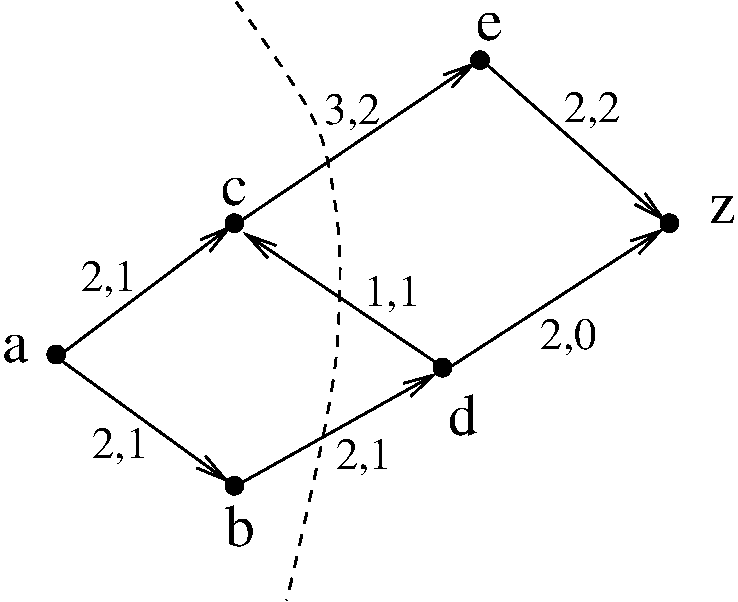
\includegraphics[width=0.3\linewidth,keepaspectratio]{snede1} % ,height=4cm}
\end{center}
\caption{A network with a flow and a cut\label{snede1}}
\end{figure}

We can check how much of the flow traverses the cut, i.e. from left to
right in the figure. While doing that, an edge from $P$ to
$\overline{P}$ should be counted as contributing to that quantity,
while the flow of the other edges must be subtracted. For the network
in Figure~\ref{snede1} we get: \mbox{$~~~~~~~~F(c,e) + F(b,d) -
F(d,c) = 2+1-1=2$ }

Comparing this number with the flow (in {\em a} or {\em z}), we notice
that these are also equal to 2! Coincidence?

We can also try to make an optimistic estimate of how much flow there
could maximally be over a cut: maybe there exists a flow that uses all
the capacity of the edges from $P$ to $\overline{P}$, and nothing is
flowing back over the other edges. We name this quantity the {\em
capacity of the cut}. In the example, we get \mbox{$~~~~~~~~C_{c,e} +
C_{b,d} = 2+3=5$}

The capacity of a cut seems larger than the flow over the cut, and
larger than the maximal flow (you can check that the maximal flow in
the example is 4). Is this a coincidence? We study this more formally.


 \begin{definition}[Capacity $C(P,\overline{P})$ of a cut]
  \textup{The \textbf{capacity of a cut} $(P,\overline{P})$ is
    $C(P,\overline{P}) = \displaystyle
    \sum_{i \in P} \sum_{j \in \overline{P}} C_{i,j}$}
\end{definition}

 \begin{theorem} \label{snedeflow}
The capacity of a cut is not smaller than a flow, i.e.
\[\sum_{i \in P} \sum_{j \in \overline{P}} C_{i,j} \geq \sum_{i \in V} F(a,i).\]
\end{theorem}
\begin{proof}
\begin{eqnarray*}
\sum_{i \in V} F(a,i) & = &
                \sum_{i \in V}(F(a,i) - F(i,a)) +
                \sum_{j \in P \backslash \{a\}} \sum_{i \in V}(F(j,i) - F(i,j))\\
        & = & \sum_{j \in P} \sum_{i \in V} (F(j,i) - F(i,j)) \\
        & = & \sum_{j \in P} \sum_{i \in P} F(j,i) +
                \sum_{j \in P} \sum_{i \in \overline{P}} F(j,i) -
                \sum_{j \in P} \sum_{i \in P} F(i,j) -
                \sum_{j \in P} \sum_{i \in \overline{P}} F(i,j)\\
        & = & \sum_{j \in P} \sum_{i \in \overline{P}} F(j,i) -
                \sum_{j \in P} \sum_{i \in \overline{P}} F(i,j)\\
        & \leq & \sum_{j \in P} \sum_{i \in \overline{P}} F(j,i)\\
        & \leq & C(P,\overline{P})
\end{eqnarray*}
\end{proof}

Note that from the last but two lines, you see that the flow equals
the flow over the cut.



A \textbf{minimal} cut is a cut with minimal capacity. The previous
theorem implies directly that any maximal flow is smaller than or
equal to the capacity of the minimal cut. The connection between the
two is even stronger:


 \begin{theorem}[Max flow - min cut \label{maxflowmincut}]
  Let $(P,\overline{P})$ be a cut and $F$ a flow in a network $G(V,E)$,
if
\[C(P,\overline{P})=F\mbox{ \ \ (or written out }
\sum_{i \in P} \sum_{j \in \overline{P}} C_{i,j} = \sum_{i \in V} F(a,i)
 \mbox{ )}\]
 then $F$ is maximal and the cut is minimal.\\
  Moreover, the equality is equivalent with
\begin{enumerate}
\item
$\forall i \in P, j \in \overline{P}: F(i,j) = C_{i,j}$ and
\item
$\forall i \in \overline{P}, j \in P: F(i,j) = 0$
\end{enumerate}
i.e. all good edges in the cut have a flow equal to their capacity and
all bad edges have zero flow.
\end{theorem}
\begin{proof}
All this follows from the inequalities in Theorem~\ref{snedeflow}
\end{proof}

Note that we have not proven that for each maximal flow there is a
minimal cut, neither the other way around.



Figure~\ref{snede2} shows a maximal flow with its minimal cut.

\begin{figure}[ht]
\begin{center}
\includegraphics[width=0.35\linewidth,keepaspectratio]{snede2} % ,height=4cm}
\end{center}
\caption{A network with a maximal flow and its minimal cut\label{snede2}}
\end{figure}

We are now ready to prove that Algorithm~\ref{maxflow} ends with a
maximal flow.



\begin{proof} (of Theorem~\ref{maxflow})\\
At the moment the algorithm ends, let $P$ be the set of vertices with
a label (note: $a \in P$) and $\overline{P}$ the set of vertices
without a label ($z \in \overline{P}$). $(P,\overline{P})$ is a cut.
Consider a (directed) edge $(i,j)$ with $i \in P$ and $j \in
\overline{P}$.  Since $i$ has a label $F(i,j)$ must be equal to
$C_{i,j}$, otherwise $j$ would have gotten a label. Now consider an
edge $(j,i)$ with $i \in P$ and $j \in \overline{P}$. Since $i$ has a
label, $F(j,i)$ must be equal to 0, otherwise $j$ would have gotten a
label. Together with Theorem~\ref{maxflowmincut}, we derive that $F$
is maximal.
\end{proof}

You see that the algorithm constructs a maximal flow
and a minimal cut at the same time. Some of the steps in Algorithm~\ref{maxflow} are
shown in Figure~\ref{maxflow1} and~\ref{maxflow2}:

\begin{figure}[ht]
\begin{center}
\subfigure[After initialisation and labeling source
a]{\includegraphics[width=0.4\linewidth,keepaspectratio]{maxflow1} \label{maxflow1}}
\hspace{1cm} \subfigure[After a labeling that reached
$z$]{\includegraphics[width=0.4\linewidth,keepaspectratio]{maxflow2} \label{maxflow2}}
\end{center}
\caption{Illustration 1 for Algorithm~\ref{maxflow}}
\end{figure}

Choose the order on the vertices as $(a,c,d,b,z)$. Starting from $a$,
$d$ and $b$ get a label. Then $c$ is labeled from $d$; $b$ is not
labeled from $d$ because $b$ has already a label. Then $z$ is labeled
from $c$: we have found a path from $a$ to $z$ as you can see in
Figure~\ref{maxflow2}. The flow is improved and the result is in
Figure~\ref{maxflow3}.

\begin{figure}[ht]
\begin{center}
\subfigure[After improving the flow the first
time]{\includegraphics[width=0.35\linewidth,keepaspectratio]{maxflow3} \label{maxflow3}}
\hspace{1cm} \subfigure[A second labeling has reached
$z$]{\includegraphics[width=0.35\linewidth,keepaspectratio]{maxflow4} \label{maxflow4}}
\end{center}
\caption{Illustration 2 for Algorithm~\ref{maxflow}}
\end{figure}

The labeling restarts in the situation of Figure~\ref{maxflow3}. From
$a$, $d$ is not labeled now: the flow on edge $(a,d)$ is already
maximal. $c$ does not get a label from $b$, because the edge $(c,b)$
is {\em bad} and its flow is zero, so it cannot be decreased. But $d$
gets a label from $b$, and since the capacity of edge $(b,d)$ (3)
is smaller than the $\Delta$ of $b$ (7 at that moment), we give $d$ a
$\Delta = 3$. $c$ gets a label from $d$ and since the unused capacity
$(d,c)$ equals 2, we give $c$ a $\Delta = 2$. From $c$, only $z$ can be
labeled: the resulting situation is in Figure \ref{maxflow4}. The flow
can be improved along the obtained path: the result is in
Figure~\ref{maxflow5}.

\begin{figure}[ht]
\begin{center}
\subfigure[After improving the flow for the second time]{\includegraphics[width=0.35\linewidth,keepaspectratio]{maxflow5} \label{maxflow5}} \hspace{1cm}
\subfigure[The labeling does not reach $z$: the cut is minimal, the
flow is
maximal]{\includegraphics[width=0.35\linewidth,keepaspectratio]{maxflow6} \label{maxflow6}}
\end{center}
\caption{Illustration 3 for Algorithm~\ref{maxflow}}
\end{figure}

At this moment, the flow is already maximal, but the algorithm has not
found that out: another attempt to construct a path from $a$ to $z$ is
needed. The last round of labeling start in the situation in Figure
\ref{maxflow5}: from $a$ we can label $b$ (the capacity of the edge
$(a,d)$ is already fully used) and also edge $(b,d)$ has some spare
capacity, but then we are stuck: the labeling stops at
Figure~\ref{maxflow6}. The minimal cut is defined by $P = \{a,b,d\}$ and
$\overline{P} = \{c,z\}$.

Run the algorithm (manually) for the networks in in
Figure~\ref{maxflow7}, with order $(a,b,c,d,e,z)$ on the vertices.

\begin{figure}[ht]
\begin{center}
\includegraphics[width=0.6\linewidth,keepaspectratio]{maxflow7} % ,height=3.2cm}
\end{center}
\caption{Two networks for practising \label{maxflow7}}
\end{figure}

Finding the maximal flow in a network is equivalent to finding
(integer) values $F(i,j)$ so that
\begin{itemize}
\item
$\sum_{j} F(a,j)$ is maximal
\item
$0 \leq F(i,j) \leq C_{i,j}$ for the given $C_{i,j}$
\item
$\forall j: \sum_{i} F(i,j) = \sum_{i} F(j,i)$
\end{itemize}

This type of problem can also be solved by linear programming,
e.g. by the simplex algorithm.

%===============================================================================
\section{Matching}

Consider the following problem: 4 students ($A,B,C$ and $D$) want to
make a separate appointment with an assistant who is available on 5
different days $(a,b,c,d$ and $e)$. Each student has their own
preference for one or more of the days. The assistant must now decide
who comes when.  Clearly, this is not always possible: e.g. if both
$A$ and $B$ have as their only preference day $a$, then it is
impossible. Even if it is possible, it is not trivial to solve such a
problem, especially not when there are many more students and days
involved.

At first sight, this problem is unrelated to graphs, but we can
represent it as a graph $G$ and work from there: the students and the
days play the role of the vertices of $G$. We draw a directed edge
between a student and a day, if that student has included that day in
their preference list. As an example: $A$ prefers $\{b,c\}$, $B$
prefers $\{a,b\}$, $C \{d,e\}$ and $D$ $\{b,c,e\}$. We get the graph
in Figure~\ref{matching1}

\begin{figure}[ht]
\begin{center}
\includegraphics[width=0.17\linewidth,keepaspectratio]{matching1} % ,height=4cm}
\end{center}
\caption{The graph for the matching problem\label{matching1}}
\end{figure}

This graph is bipartite and directed. The connection with the previous
section becomes clear if we add a source and a sink, and give each
edge 1 as capacity: see Figure~\ref{matching2}.

\begin{figure}[ht]
\begin{center}
\includegraphics[width=0.5\linewidth,keepaspectratio]{matching2} % ,height=4cm}
\end{center}
\caption{Network for the matching problem: all edges have capacity =
1\label{matching2}}
\end{figure}

We can now construct a maximal (integer) flow $F$ in in this network:
the value of this maximal flow is 4 (the number of students). We can
derive an assignment of students to days (or a matching of the
students with the days) by interpreting an edge $(s,d)$ so that
$F((s,d)) = 1$ as: student $s$ can see the assistant on day
$d$. Figure~\ref{matching3} shows a maximal flow with dotted lines. From this, we
can read out the assignment $(A,b)$, $(B,a)$, $(C,d)$,
$(D,e)$. The assignment is complete, and we have a complete (or
perfect) matching, since every student is matched up with a day.

\begin{figure}[ht]
\begin{center}
\includegraphics[width=0.5\linewidth,keepaspectratio]{matching3} % ,height=4cm}
\end{center}
\caption{A solution for the assignment problem\label{matching3}}
\end{figure}

The maximal flow could have been smaller than the number of
students (for a different set of preferences of course): that maximal
flow gives us a maximal matching, but not a complete one. More
formally:


 \begin{definition}
{\rm Let $G(V \cup W,E)$ be a directed, bipartite graph $G(V \cup
W,E)$ with $V \cap W = \emptyset$ and $E \subseteq V \times W$, then
$M$ is a \textbf{matching} if
\begin{verse}
\hspace*{1ex}$\bullet$
$M \subseteq E$ and

\hspace*{1ex}$\bullet$
$\forall (x,y),\;(i,j) \in M:$ if $(i,j) \neq (x,y)$ then
$i \neq x$ and $j \neq y$
(i.e. at most one edge arrives and leaves any vertex)
\end{verse}
A \textbf{maximal} matching has a maximal number of edges in $M$. A
matching is \textbf{complete} if $\forall v \in V,\; \exists w\in W:\;
(v,w) \in M$.  }
\end{definition}

A directed, bipartite graph $G(V \cup W,E)$ to which a source and sink
are added, with edges from the source to all the vertices in $V$, and edges from
all the vertices in $W$ to the sink, with a capacity of 1 for every
edge is named the \textbf{matching network} derived from $G$.


The next theorem formalises the correspondence between a maximal
flow in a matching network and a maximal matching.

 \begin{theorem}
Let $G(V \cup W,E)$ be a directed, bipartite graph
with $V \cap W = \emptyset$ and $E \subseteq V \times W$, then the
following is true:
\begin{verse}
\hspace*{1ex}$\bullet$
An integer flow in the corresponding matching network $F$ gives a
matching in $G$: $v \in V$ corresponds to $w \in W$ if and only if
$F(v,w) = 1$

\hspace*{1ex}$\bullet$
A maximal integer flow corresponds to a maximal matching.

\hspace*{1ex}$\bullet$
An integer flow with value $\#V$ corresponds to a perfect matching.
\end{verse}
\end{theorem}
\begin{proof}
You can work out the proof yourself.
\end{proof}

It is sometimes possible to quickly test that no perfect matching
exists: clearly, when $n$ students together prefer strictly fewer than
$n$ days, they cannot all get one of their preferred days. We generalize this:

\begin{itemize}
\item
define the mapping \footnote{${\cal P}(S)$ denotes the power set of
$S$}

\begin{center}
$
\begin{array}{lrcl}
R: & {\cal P}(V) & \rightarrow & {\cal P}(W)\\
   & S    & \mapsto     &
                \{w\in W \;|\; \exists v \in S \mbox{ with }(v,w) \in E\}
\end{array}
$
\end{center}
\item
If $G$ has a perfect match, then $\#S \leq \#R(S)$ holds $\forall S
\subseteq V$
\end{itemize}

The English mathematician Philip Hall proved the converse in 1935:

 \begin{theorem}[Hall's marriage theorem \label{hall}]

A directed, bipartite graph $G(V \cup W,E)$ with $V \cap W =
\emptyset$ and $E \subseteq V \times W$, has a perfect match if and
only if $\#S \leq \#R(S),\; \forall S \subseteq V$
\end{theorem}
\begin{proof}
We have already argued one direction: if $G$ has a perfect match, then
$\#S \leq \#R(S), \forall S \subseteq V$. Now the converse:

Let $m = |V|$. We prove by induction on $m$ that the condition is
sufficient. The base case is $m=1$: it is clear that a perfect match
exists. So assume $m \geq 2$. We distinguish between two cases:


\begin{enumerate}
\item
Suppose that for all $S$ such that $\emptyset \neq S \subsetneq V$ it
is true that $|S| + 1 \leq |R(S)|$. Take any edge $(v,w)$ with $v \in
V$ and consider the $G' = G \setminus \{v,w\}$. $G'$ fulfills the
conditions of Hall and $V'$ is strictly smaller than $m$: by the
induction hypothesis there exists a perfect matching of $G'$. Add the
edge $(v,w)$ to it and obtain a perfect match of $G$.

\item
Now assume the existence of a set $S$ with $\emptyset \neq S
\subsetneq V$ and $|S| = |R(S)|$. Consider the subgraph $G_1$ induced
by the vertices $S \cup R(S)$, and the subgraph $G_2$ induced by
$(V\setminus S) \cup (W \setminus R(S))$. Now prove that $G_1$ and
$G_2$ fulfill the conditions of Hall, so they both have a perfect
matching. Take the union of these perfect matchings to obtain a perfect
matching of $G$. Figure \ref{hallfig} illustrates the construction.
\end{enumerate}
\end{proof}

\begin{figure}[h]
\begin{center}
\includegraphics[height=0.35\textheight,keepaspectratio]{hall}
\caption{The dashed lines belong to the original graph, but not to $G_1$ and $G_2$}\label{hallfig}
\end{center}
\end{figure}

Hall's Theorem~\ref{hall} can be used in partner choice problems, hence its name.



% http://myweb.facstaff.wwu.edu/sarkara/hall.pdf geeft een mooier bewijs
% van de stelling van Hall, eentje waarvoor geen kennis van networken
% nodig is.





\addtocontents{toc}{\protect\vspace{10pt}}

\part{Languages \& Automata}

\graphicspath{{./LanguagesAutomata/figures/}}

\chapter{Introduction to Languages and Automata}\label{chap:languagesautomaten}

Computer programs are central in the activity of the computer
scientist. Computer programs transform a given input into a desired
output. The input could be an electric pulse indicating a temperature
change, a character from the keyboard, another program, a database
\ldots The output could be a sequence of signals controlling some valves,
a new version of a document, an error message, the display of a
graph \ldots

From a practical point of view, the above examples are quite
different, but when we focus too much on the details, we miss a lot.
We can abstract away many details and focus on the essence: in every
example, there is a mapping from elements in an input domain to
elements in an output domain. These domains are always discrete, and
sometimes infinite. This means that from a theoretical point of view,
programs are just functions from (a part of) $\N$ to (a part of) $\N$.

In case the input domain is small, that function is not very
interesting: one could just build a table with all precomputed values,
and then the computation is just a simple lookup.\footnote{Tabulation
is an interesting dynamic implementation technique, whichever the
programming paradigm. Ask if you want to know more.}

In case the input domain is large, or not a priori known, then it is
impossible to tabulate the function, so it is better to assume the
input domain is infinite.

Now about the output domain: it needs to contain at least two values
to be interesting. These two elements could be {\em yes, no} and that
is enough to describe {\em decision problems}: you want to know
whether a given input has a certain property, e.g. {\em is this
program syntactically correct?} or {\em is this a good day to invest
time in FCS?} \footnote{Yes !}  \ldots

If the output domain contains more than two elements, but a finite
number of them, then one can easily compute the correct output by a
finite sequence of yes/no questions. Suppose you want to know which is
the best day of the week for investing time in FCS (the output domain
has 7 values), you could ask the following yes/no questions {\em is
Monday the best day for investing time in FCS?}, {\em is Tuesday the
best day for investing time in FCS?} \ldots So, it seems that of all
finite output domains, the only really interesting one has exactly two
values.

If the output domain is infinite, the function can not be reduced
easily to a finite sequence of functions with a finite output domain.

We can conclude that there exist only two kinds of interesting
functions. They have signature $\N \rightarrow\{yes, no\}$ and $\N \rightarrow \N$.

We focus for now on the first kind: it is easy to associate a certain
structure and semantics with the output domain, but the input domain
is very generic. $\N$ could indeed be replaced by any other countably
infinite set. Moreover, when we note down elements of $\N$, we can use
decimal digits: we form strings (sequences) of such digits. We could
have used another basis for the representation - binary, hexadecimal,
or even more exotic excess-3, \ldots These representations have something
in common: a finite set of symbols is used (we name it an alphabet), a
sequence of such symbols (we name it a string) has a unique meaning,
and one can concatenate strings.
%
Let $\Sigma$ denote a finite alphabet, and let $\Sigma^*$ denote all
finite sequences of symbols from $\Sigma$. Then we have just argued
that the interesting functions have signature $\Sigma^* \rightarrow
\{yes, no\}$. A function $F$ in this class is totally determined by the
set of strings $s$ for which $F(s) = yes$, so instead of studying such
functions, we can just as well study subsets $V$ of $\Sigma^*$
together with the associated question: {\em does a given s belong to
$V$}. It is important to understand that we are still considering the
same class of functions $\N \rightarrow\{yes, no\}$, but also that it
is often more natural and insightful to describe decision problems
starting from a particular $\Sigma^*$. Almost all of computability
theory uses this framework.

The second kind of functions - the ones with signature $\N \rightarrow
\N$ - are of course very important as well, but will not be the focus
in this course.


{\bf Selfie:}
\begin{itemize}
\item[]
The introduction simplifies matters, and makes assumptions that you
might disagree with, or that require a bit more argument ... Find {\em
holes} in the introduction, think of alternatives, argue in favor and
against ...

Describe a decision problem already known to you, but now by choosing
an alphabet $\Sigma$ and defining a subset $Sol$ of $\Sigma^*$ that is
the solution to the problem. Do that for different kinds of problems:
with numbers, words, graphs, ... Make sure to construct an example in
which $Sol$ is finite and one in which it is infinite. What happens if
you interchange $yes$ and $no$?

\end{itemize}

\newpage
\section{What Is a Language?}

The introduction gives the motivation for studying decision
problems. A decision problem corresponds to a subset of all strings
(or words) consisting of elements of a finite alphabet $\Sigma$. Any
such subset is a {\em language} over $\Sigma$.

\begin{definition}[String over an alphabet $\Sigma$]
A {\bf string} over an alphabet $\Sigma$ is a finite sequence of zero,
one or more elements of $\Sigma$.
\end{definition}

Clearly, if we put two strings $x$ and $y$ one after the other, we get
a new string denoted $xy$.

\begin{definition}[Language over an alphabet $\Sigma$]
A {\bf language} over an alphabet $\Sigma$ is a set of (finite)
strings over $\Sigma$.
\end{definition}

A language can be finite or infinite. If the language $L$ is infinite,
is it countably infinite?\footnote{If you do not remember what that
means, now is the time to look it up}

In order to identify a language, one must give a description for every
element of the language, and that description should not fit any
string not in the language. E.g. the language of odd numbers (over the
alphabet of decimal digits), or the set of strings ending on
1,3,5,7,9. Another example: the English words rhyming with automata.

The description of a language is preferably finite, even if the
language itself is infinite.

The description of the language can {\em often} be used to check whether a
given string belongs to the language, and even to generate or
construct each element of the language. But be careful with the {\em
often}: we will need to get back to it.

If the description of a language is simple, we expect the language to
be simple, but we don't really have a good idea what {\em simple}
means here.

Here are some questions for you to think about: this course provides
you with material to answer them.

\begin{itemize}
\item
Do formalisms exist that can denote language descriptions?

\item
Does such a formalism allow to (automatically) derive testers and
generators for the language?

\item
Are there languages that do not fit the formalism?

\item
What is a good notion of testing/generating?

\item
Are some languages inherently easier to describe, test, generate?

\end{itemize}

And finally:

\begin{itemize}
\item[] Why should a computer scientist know all this?
\end{itemize}


\paragraph{Selfie:}
\begin{itemize}
\item[]

Can you use the description of the set of even numbers to generate all even numbers?

Same question but for the English words rhyming with automata.

Can you use them for testing?

Invent a new very extravagant language, give its description and use
it to test whether a given string belongs to it, and use it to
generate all strings belonging to the language.

Based on these examples, can you see a connection between the ease of
description, the testing and the generation?
\end{itemize}

%===============================================================================
\section{An Algebra of Languages}

An algebra (or algebraic structure) is a set with some internal
operations (often binary operations, but unary operations are also
common, and even operations with a larger arity). The set of languages
over the alphabet $\Sigma$ becomes an algebra by defining operations
like union, intersection, complement \ldots More concrete:
let $L_1$ and $L_2$ be two languages, then

\begin{itemize}
\item their union is a language: $L_1 \cup L_2$
\item their intersection is a language: $L_1 \cap L_2$
\item the complement is a language: $\overline{L_1}$
\end{itemize}

You can construct other operations on languages by composing the three
above, just like with any sets.

There is also a new way - not directly linked to set theory - to make
a new language out of two given languages: {\em concatenation}.

\begin{definition}[Concatenation of two languages]
Let $L_1$ and $L_2$ be two languages over the same alphabet $\Sigma$,
then we denote the concatenation of $L_1$ and $L_2$ by $L_1L_2$ and we
define: $L_1L_2 = \{xy | x \in L_1, y \in L_2\}$.
\end{definition}

When we concatenate three languages, we do not need brackets, because
clearly, concatenation is associative:
%
$(L_1L_2)L_3 = L_1(L_2L_3)$


Concatenating $L$ n times with itself is denoted by $L^n$.
$L^0$ contains only the empty string, and we denote that string by
$\epsilon$.

Finally, we also define an operation that allows to construct an
infinite language from a finite one:

\begin{definition}[$L^*$ - the Kleene {\bf star} of $L$]
$L^* = \cup_{n=0}^\infty L^n$
\end{definition}

As an abbreviation of $LL^*$ one uses $L^+$.


Now we have all this notation, we can say that $L$ is a language over
$\Sigma$ if $L \subseteq \Sigma^*$, or equivalently
%
$ L \in {\cal P}(\Sigma^*)$.

\paragraph{Selfie:} Define new operations on languages.

%===============================================================================
\section{Language Descriptions}

In maths, one uses the set notation, e.g.

\begin{example}
Let $\Sigma = \{x,y,z\}$:
\begin{itemize}
\item
$\Sigma^* = \{a_1a_2a_3...a_n|~a_i \in \Sigma, n \in \N \}$
\item
$L = \{a_1a_2a_3...a_n|~a_1 = y, n \in \N, \forall i > 1: a_i \in \Sigma\}$

or in words: L is the set of strings starting with y
\end{itemize}
\end{example}

Informal descriptions are possible as well, as long as they are not
ambiguous about membership.

\begin{example}
~~
\begin{itemize}
\item
$H(n) = \{P | P~is~a~Java~program~and~P~stops~after~at~most~~n~seconds~on~input~n\}$
\item
$Prime = \{n|n \in \N, n~is~prime\}$
\end{itemize}
\end{example}

While the last one is an informal description, it hides the formal
description of {\em prime}, so we could also have specified $Prime$ as

\hspace{1cm}$Prime = \{n|n \in \N, \forall i:1<i<n \rightarrow n~mod~i \neq 0\}$

This kind of description is OK for doing maths, but computer
scientists need a different formalism: it should (more easily) allow
to convert a description into a generator and a tester. For natural
languages, linguists have grammars: they describe the structure of a
sentence. Natural languages are very complicated, with lots of
exceptions to rules, and exceptions to exceptions \ldots It makes sense
to study classes of languages with a simpler structure. We aim
therefore at

\begin{itemize}
\item[]
a hierarchy of languages

\item[]
an accompanying hierarchy of description formalisms, or grammars

\item[]
an accompanying hierarchy of {\em test} and {\em generate} procedures

\end{itemize}

The hierarchy we study is named the {\em
Chomsky-hierarchy\footnote{Noam Chomsky}}. We start at the bottom of
this hierarchy, i.e. with the easiest languages.



%///////////////////////////////////////////////////////////////////////////////
\chapter{Regular Expressions and Regular Languages}

%===============================================================================
\section{Basic Definitions}

\begin{definition}[Regular Expression (RE) over an alphabet $\Sigma$] \label{defregexp}
E is a {\bf regular expression over alphabet $\Sigma$} if E has the form
\begin{itemize}
\item $\epsilon$
\item $\phi$
\item $a$ for $a \in \Sigma$
\item $(E_1E_2)$ for regular expressions $E_1$ and $E_2$ over $\Sigma$
\item $(E_1)^*$ for a regular expression $E_1$ over $\Sigma$
\item $(E_1 | E_2)$ for regular expressions $E_1$ and $E_2$ over $\Sigma$
\end{itemize}
\end{definition}

In this way, the set of regular expressions {\em RegExps} (over an
alphabet $\Sigma$) is defined inductively. It implies that something
that does not comply with the definition is not a regular expression,
and that every regular expression can be constructed using only the
rules above.
%
It is often implicitly clear which alphabet is used, and we often do
not mention it.
%
We use the brackets to avoid ambiguity: the brackets to not belong to
the alphabet.
%
In the next examples, $\Sigma = \{a,b,c\}$.

\begin{example}
Regular expressions over $\Sigma$:
\begin{itemize}
\item b
\item a($\epsilon$c)
\item $(((ab))^*c~|~(bc))$
\end{itemize}
\end{example}

Are we using too many brackets, too few? Why?

\begin{definition}
A regular expression E {\bf determines} a
language $L_E$ over its alphabet $\Sigma$ as follows:
\begin{itemize}
\item if E = a ($a \in \Sigma$) then $L_E = \{a\}$ (the language with
just one string, consisting of the character a)
\item if E = $\epsilon$ then $L_E = \{\epsilon\}$ (the empty string)
\item if E = $\phi$ then $L_E = \emptyset$ (the empty set)
\item if E = $(E_1E_2)$ then $L_E = L_{E_1}L_{E_2}$
\item if E = $(E_1)^*$ then $L_E = L_{E_1}^*$
\item if E = $(E_1 | E_2)$ then $L_E = L_{E_1} \cup L_{E_2}$
\end{itemize}
\end{definition}

This similarity between the structure of the regular expressions and
the structure of the languages they determine is not a coincidence,
and we can exploit it to use less brackets in regular expressions. We
just agree that $^*$ takes precedence over concatenation, which takes
precedence over union. Note also that concatenation is associative. So
we can agree that $L_{(((a)^*(b))c)} = L_{a^*bc}$. You should however
never say that the regular expression $(((a)^*(b))c)$ equals the
regular expression $a^*bc$: the correct wording is {\em the language
(determined by) $(((a)^*(b))c)$ equals the language (determined by)
$a^*bc$}.

\paragraph{Selfie:}
Formulate a verbal description of the languages determined by the REs
over $\{a,b\}$ below - the first one is an example:

\begin{itemize}
\item[]
$(ab)^*$: every $a$ is followed immediately by a $b$, and there are as
many $a$'s as $b$'s

$(aba)^*$

$(a|b)^*$

$(a|b)^*\phi$

$a \epsilon b$
\end{itemize}

\paragraph{Selfie:}
Prove the following statements, or give a counterexample:

\begin{itemize}
\item[]
if a regular expression E does not contain a $^*$, then $L_E$ is
finite

if a regular expression E contains a $^*$, then $L_E$ is infinite

$L_E \subseteq L_{(E|F)}$ for all RE's E and F

the set of regular expressions (over a given alphabet) is itself a
language (over which alphabet?)
\end{itemize}


\medskip

\begin{definition}[Regular Language]
A language determined by a regular expression is named a {\bf regular language}.
\end{definition}

We denote the set of regular languages by $RegLan$. Check which of the
formulas below make sense, and which are true.

\begin{enumerate}
\item $RegLan \subseteq \Sigma$
\item $RegLan \subseteq \Sigma^*$
\item $RegLan \subseteq {\cal P}(\Sigma)$
\item $RegLan \subseteq {\cal P}(\Sigma^*)$
\item $RegLan \subseteq {\cal P}({\cal P}(\Sigma^*))$
\item if $x \in RegLan$ then $x \in \Sigma$
\item if $x \in RegLan$ then $x \in \Sigma^*$
\item if $x \in RegLan$ then $x \in {\cal P}(\Sigma)$
\item if $x \in RegLan$ then $x \in {\cal P}(\Sigma^*)$
\item if $x \in RegLan$ and $y \in x$ then $y \in \Sigma$
\item if $x \in RegLan$ and $y \in x$ then $y \in \Sigma^*$
\item if $x \in RegLan$ and $y \in x$ then $y \in {\cal P}(\Sigma)$
\item if $x \in RegLan$ and $y \in x$ then $y \in {\cal P}(\Sigma^*)$
\end{enumerate}

\paragraph{Selfie:}

\begin{itemize}
\item[]
Is true that {\em for every regular language L, there exists a regular
expression E so that $L_E = L$}?


Is it clear that there exist languages that are NOT regular?

Is every finite language regular?

Is every infinite regular language countable?

Given a regular language, can you construct (one of) its regular
expression(s)?

For given string $s$ and regular expression $E$, can you
determine whether $s \in L_E$?

Can you generate all strings in $L_E$ once you have $E$?
\end{itemize}


\section{The Subalgebra of Regular Languages}

We denote the set of languages over alphabet $\Sigma$ by
$L_\Sigma$. It is an algebra for certain operations, and
%
$L_\Sigma = {\cal P}(\Sigma^*)$.

For $L_1, L_2 \in L_\Sigma$, we can consider the language $L_1L_2$
(concatenation), $L_1 \cup L_2$ (union), $L_1^*$ (repetition), and
$\overline{L_1}$ (complement). The result is always a member of
$L_\Sigma$. We say: $L_\Sigma$ is an algebra with (at least) four
internal operations.

Since $RegLan$ is a subset of $L_\Sigma$, it makes sense to ask whether
RegLan is a subalgebra of $L_\Sigma$. In other words: are the
operations internal to RegLan?

\paragraph{Selfie:} Formulate a theorem stating that RegLan is a
subalgebra of $L_\Sigma$ (for the four operations above), and prove it
in a constructive way, i.e. (for union) construct an E so that $L_E =
L_{E_1} \cup L_{E_2}$. Did you succeed for complement?




\section{Finite Automata}

Finite state machines (FSM) are used to describe languages: testing
and generating strings is part of that. We start with a
graphical representation of an FSM. The formal definition follows
later. Figure~\ref{fsa1} shows a first example of an {\em
  NFA} \footnote{The explanation of this acronym follows later.} over
the alphabet $\{a,b,c\}$.

\begin{figure}[h]
\begin{center}\includegraphics[%
  width=0.5\linewidth,
  keepaspectratio]{fsa1}\end{center}
\caption{A finite state machine\label{fsa1}}
\end{figure}

The most important characteristics are:

\begin{itemize}
\item we see a directed graph
\item the vertices have a name (in this case a number) - the vertices
  are named {\em states}
\item there are two kinds of states: states with a double circle are
  named accepting states (sometimes also named end states or final
  states)
\item loops are allowed
\item the edges are labelled with zero, one, or more symbols from the
  alphabet, and/or $\epsilon$
\item there is exactly one edge not starting from a vertex: the vertex
  in which it arrives is named the start state
\end{itemize}

We can use this graphical representation as follows:

\begin{enumerate}
\item you get a string $s$ over the alphabet (it is now your current
  string) and you start in the start state
\item you can now go from one state to the other along any given
  edge but you must pay a price for that: you spend from the beginning
  of your current string a symbol that appears on the edge (meaning
  that your string shortens); in case the edge contains $\epsilon$,
  you do not need to spend a symbol from your string
\item if you manage to arrive in a final state with an empty string,
  we say {\em the NFA accepts the initial string $s$}
\end{enumerate}

This constitues only an informal definition of which strings are
accepted by an NFA.

Here is a different use of the graphical representation:

\begin{enumerate}
\item start with an empty string in the start state: that is your
  current string
\item now follow any edges: if the edge has a label with symbols from
  the alphabet, add any of these symbols to you string; if the edge
  contains $\epsilon$ you don't have to add any symbol; keep doing that
\item any time you arrive at a final state, you may say {\em this machine generates the current string}
\end{enumerate}



\paragraph{Selfie:} Answer the following questions:

\begin{itemize}
\item[]
does the NFA in Figure~\ref{fsa1} accept ac?

does the NFA in Figure~\ref{fsa1} accept bbb?

is there more than one way to accept bbb?

is it possible that you get stuck with bbb and what does that mean for bbb?

can you give some strings not accepted by this NFA?

construct an NFA with a circuit - can you now get into an endless
loop? is that a problem?

can you comment on {\em the set of strings generated by the NFA equals
  the set of strings accepted by the NFA} ?
\end{itemize}

\begin{definition}[An NFA M determines a language (informal)]
A language L is determined by the NFA M, if M accepts every string
from L, and no other strings. We denote this language by $L_M$.
\end{definition}

The alphabets of the NFA and the language do not need to be the same,
but it is convenient to assume they are.

\begin{definition}[Equivalence of NFAs]
Two NFAs are {\bf equivalent} if they determine the same language.
\end{definition}

The relation {\em NFA-equivalence} defines an equivalence relation on
NFAs: each equivalence class corresponds to one language.


\paragraph{Selfie:} think about the following

\begin{itemize}
\item[] there exists a procedure for deciding whether two given NFAs
  are equivalent

for each NFA there exists an equivalent one with at most one final
state

for each NFA there exists an equivalent one in which {\em you can't
  get stuck}
\end{itemize}

We often need the set $\Sigma \cup \{\epsilon\}$: we abbreviate it by
$\Sigma_\epsilon$.

\begin{definition}[Non-deterministic finite state automaton] \label{nfadef}
A {\bf non-deterministic finite state automaton} is a 5-tuple
$(Q,\Sigma,\delta,q_s,F)$ with
\begin{itemize}
\item Q a finite set of states
\item $\Sigma$ a finite alphabet
\item $\delta$ a transition function, i.e.
%
$\delta: Q \times \Sigma_\epsilon \rightarrow {\cal P}(Q)$
\item $q_s$ is the start state and an element of $Q$
\item $F \subseteq Q$: F is the set of final states
\end{itemize}
\end{definition}

As you guessed by now: NFA is an acronym of {\em Non-deterministic Finite
  Automaton}.


We formally define what it means for a string $s$ to be accepted by an
NFA.

\begin{definition}[A string accepted by an NFA] \label{defacceptnfa}
A string $s$ is accepted by an NFA
$(Q,\Sigma,\delta,q_s,F)$ if $s$ can be written as
$a_1a_2a_3...a_n$ with $a_i \in \Sigma_\epsilon$, and there
exist a sequence of states $t_1t_2t_2t_3...t_{n+1}$ so that
\begin{itemize}
\item $t_1 = q_s$
\item $t_{i+1} \in \delta(t_i,a_i)$
\item $t_{n+1} \in F$
\end{itemize}
\end{definition}

\newpage
\paragraph{Selfie:}
\begin{itemize}
\item[]
You now have both an intuitive notion of acceptance by an NFA (through
its graphical representation) and a formal definition: make sure that
your intuition matches the definition.
\end{itemize}


Up to now, we have defined only non-deterministic automata: it is
possible that at a particular state, there is more than one outgoing
edge with the same symbol. This leaves a potential choice. But some of
those NFAs are deterministic: there is no choice. Such an automaton is
a DFA.

The next section shows the connection between regular expressions and
NFAs: we first construct an NFA from a RE so that $L_{RE} = L_{NFA}$,
and later we do the reverse. Together, this will prove that the two
formalisms are (in some sense) equivalent.


\section{The Transition Table}

The $\delta$ of an NFA is a function with a finite domain. It can be
represented in the form of a table named the {\em transition table}:
it shows which transitions are possible in the NFA. As an example:

\begin{table}[ht]
\center
\begin{tabular}{|r|r|r|}
\hline
$Q$    & $\Sigma_\epsilon$ &  ${\cal P}(Q)$ \\ \hline
1      & a                  &  $\{2\}$         \\
1      & b                  &  $\{3\}$         \\
1      & $\epsilon$         &  $\{2\}$         \\
2      & a                  &  $\{2\}$         \\
2      & b                  &  $\{2,4\}$         \\
3      & a                  &  $\{3\}$         \\
3      & b                  &  $\{3\}$         \\ \hline
2      & $\epsilon$         &  $\emptyset$         \\
3      & $\epsilon$         &  $\emptyset$         \\
4      & a                  &  $\emptyset$         \\
4      & b                  &  $\emptyset$         \\
4      & $\epsilon$         &  $\emptyset$         \\
1,2,3,4 & c                 &  $\emptyset$         \\
\hline
\end{tabular}
\caption{The transition table of the NFA in
Figure~\ref{fsa1}} \label{transitietabel}
\end{table}

For a combination of a state in the NFA and a symbol in
$\Sigma_\epsilon$ for which there is an edge in the graphical
representation, there is a set of states to which transition is
possible. When there is no edge, one can add the entry with an empty
set of states.

The transition table definitely looks usable in a program that
implements the NFA. The non-determinism is perhaps a bit scary, but
don't panic: we will get rid of it.




\section{An Algebra of NFAs}

We fix the alphabet: we might relax this later. The set of NFAs
over this alphabet is well defined: use the definition on page
\pageref{nfadef}. We will show that on this set, we can define three
internal operations: two binary ones (union and concatenation) and a
unary one (the star). In the mean time, you know that an NFA can
always be transformed to an equivalent one with exactly one accepting
state from which no edges leave. That will make things a little easier.

\paragraph{The union of two NFAs:}


Figure~\ref{uniefsa} shows the intuition about the union of two NFAs:
construct a new accepting state and draw an $\epsilon$-edge from the
old end states to the new one; the old end states become
non-accepeting. Construct a new starting state, with $\epsilon$-edges
to the old starting states.


\begin{figure}[h]
\begin{center}\includegraphics[%
  width=0.6\linewidth,
  keepaspectratio]{uniefsaeng}\end{center}
\caption{The union of two NFAs\label{uniefsa}}
\end{figure}

We can write formally:

Given $NFA_1 = (Q_1,\Sigma,\delta_1,q_{s1},\{q_{f1}\})$ and
%
$NFA_2 = (Q_2,\Sigma,\delta_2,q_{s2},\{q_{f2}\})$.

The union $NFA_1 \cup NFA_2$ is an $NFA = (Q,\Sigma,\delta,q_s,F)$
in which
\begin{itemize}
\item $Q = Q_1 \cup Q_2 \cup \{q_s,q_f\}$ with $q_s$ and $q_f$ new states
\item $F = \{q_f\}$
\item $\delta$ is defined as

 $\delta(q,x) = \delta_i(q,x)~~\forall q \in Q_i \backslash \{q_{fi}\}, x \in \Sigma_\epsilon$ for i=1,2 \\
 $\delta(q_s,\epsilon) = \{q_{s1}, q_{s2}\}$ \\
 $\delta(q_s,x) = \emptyset ~~\forall x \in \Sigma$ \\
 $\delta(q_{fi},\epsilon) = \{q_f\}$ for i = 1,2 \\
 $\delta(q_{fi}, x) = \emptyset ~~\forall x \in \Sigma$ and for i = 1,2
\end{itemize}


\paragraph{The concatenation of two NFAs:} this time we just give the
graphical representation of concatenation in Figure~\ref{concatfsa}:

\begin{figure}[h]
\begin{center}\includegraphics[%
  width=0.6\linewidth,
  keepaspectratio]{concatfsaeng}\end{center}
\caption{Concatenation of two NFAs\label{concatfsa}}
\end{figure}


\paragraph{The star of an NFA:} see Figure~\ref{starfsa}.

\begin{figure}[h]
\begin{center}\includegraphics[%
  width=0.6\linewidth,
  keepaspectratio]{sterfsaeng}\end{center}
\caption{The star of an NFA\label{starfsa}}
\end{figure}

You should work out the formal description of concatenation and star
yourself.

\paragraph{Selfie:}
\begin{itemize}
\item[]
The concatenation of $NFA_1$ and $NFA_2$ determines
$L_{NFA_1}L_{NFA_2}$: prove this.

Formulate a similar statement for star and union.

What does this prove about the algebraic isomorphism between ... and ... ?

\end{itemize}



\section{From Regular Expression to NFA}\label{re2fsasec}

We now have all the necessary ingredients to construct an NFA from a regular
expression RE such that $L_{RE} = L_{NFA}$. Since regular
expressions are defined inductively (see definition page
\pageref{defregexp}) we define a corresponding NFA for each case in the
definition. $NFA_{RE}$ denotes the NFA corresponding to a
regular expression RE.

Figure~\ref{re2fsa} shows the NFA for the first three bases cases in
the definition on page \pageref{defregexp}:

\begin{figure}[h]
\begin{center}\includegraphics[%
  width=0.55\linewidth,
  keepaspectratio]{re2fsa}\end{center}
\caption{An NFA for the three base cases\label{re2fsa}}
\end{figure}

The three {\em recursive} cases are described as follows: let $E_1$
and $E_2$ be two regular expressions, then
\begin{itemize}
\item $NFA_{E_1E_2} = concat(NFA_{E_1},NFA_{E_2})$
\item $NFA_{E_1^*} = star(NFA_{E_1})$
\item $NFA_{E_1|E_2} = union(NFA_{E_1},NFA_{E_2})$
\end{itemize}

\begin{theorem}
The construction above preserves the language, i.e.

~~~~~~~~~~~~~~~~~~~~~~~~~~~~~~~~~~~~~~~ $L_{NFA_E} = L_E$.
\end{theorem}
\begin{proof}
Prove this yourself - use structural induction.
\end{proof}


\section{From NFA to Regular Expression}

The opposite way is a bit more complicated: we first introduce a new
kind of finite automata, the {\em Generalized Non-deterministic Finite
Automata} or GNFAs. We will then follow the path:


$NFA \rightarrow GNFA \rightarrow GNFA~with~2~states \rightarrow regular~expression$

In each of the steps, we must prove that the language stays the same.

\begin{definition}[GNFA (informal)]
A {\bf GNFA} is a finite state machine with the following
modifications and restrictions:
\begin{itemize}
\item there is exactly one end state and it differs from the start state
\item there is exactly one edge from the start state to any other
state, but the start state has no incoming edge (except for the start arrow)
\item there is exactly one edge from each state to the end state, but
the end state has no outgoing edge
\item there is exactly one edge between every other two states (in both
directions) and an edge from each state to itself
\item the edges carry a regular expression as a label
\end{itemize}
\end{definition}


Figure~\ref{gfsa1} shows a GNFA.

\begin{figure}[h]
\begin{center}\includegraphics[%
  width=0.5\linewidth,
  keepaspectratio]{gfsa1}\end{center}
\caption{A GNFA\label{gfsa1}}
\end{figure}

We use the (graphical representation of the) GNFA as follows:

\begin{enumerate}
\item you start off with a string $s$ in the start state
\item you may now move to any state (the same or another one) by
following an edge as long as your string starts with a substring that
matches the regular expression on the edge: during the transition, you
chop off that substring; if the regular expression equals $\epsilon$,
the substring has length zero; if the edge just contains $\phi$, you
can't take that edge
\item keep making transitions: if you arrive in the end state with an
empty string, we say {\em the GNFA has accepted the initial string $s$}
\end{enumerate}

% \newpage
\paragraph{Selfie:}
\begin{itemize}
\item[]
For the GNFA in Figure~\ref{gfsa1}, find strings accepted by it and
strings not accepted by it.
\end{itemize}



Now is the time to describe an algorithm for constructing a RE from an NFA.

\begin{itemize}
\item[Step 1:]  {\em Make a GNFA from an NFA}

Introduce a new start state and a new unique end state. Draw an
$\epsilon$-edge from the new start state to the old start state. and
from the old end states to the new end state. Draw all missing edges
with label $\phi$. Replace parallel edges into a new edge with as
label the union of the labels of the parallel edges.

\item[Step 2:]  {\em Reduce the GNFA to a GNFA with two states}

Choose any state X different from start and end state: if there is
none, go to step 3. Remove X and for each pair of states A and B with
an edge
% from
A to X with $E_1$,
%
from X to itself with $E_2$,
%
from X to B with $E_3$,
%
from A to B with $E_4$,
%
replace the label on the edge from A to B by
$E_4~|~E_1E_2^*E_3$. Finally, remove all edges connected to X.

This base step is illustrated in Figure~\ref{redgfsa1}.

Repeat step 2.

\begin{figure}[h]
\begin{center}\includegraphics[%
  width=0.6\linewidth,
  keepaspectratio]{redgfsa1}\end{center}
\caption{Removal of one state from the GNFA \label{redgfsa1}}
\end{figure}


\item[Step 3:]  {\em Determine the RE}

The GNFA has exactly two states: the start and the accepting
state. There is only one edge and it has RE as a label.
\end{itemize}


\paragraph{Example:} Figures~\ref{gfsa2}~and~\ref{gfsa3} illustrate
this on the GNFA of Figure~\ref{gfsa1}.


\begin{figure}[h]
\begin{center}\includegraphics[%
  width=0.6\linewidth,
  keepaspectratio]{gfsa2}\end{center}
\caption{State 2 was removed \label{gfsa2}}
\end{figure}

\begin{figure}[h]
\begin{center}\includegraphics[%
  width=0.6\linewidth,
  keepaspectratio]{gfsa3}\end{center}
\caption{State 3 was removed \label{gfsa3}}
\end{figure}


The main thing to prove is that the elimination of X in
Step 2 does not change the set of accepted strings. We need to prove
two things: (1) if a string $s$ was accepted before the elimination,
it is also accepted after elimination; (2) if a string was not accepted
before elimination, it is not accepted afterwards.

% \newpage

We use the notion of a path through the GNFA that can be followed to
accept a string - the related notion for NFAs can be found on page
\pageref{defacceptnfa}: write it out for a GNFA. Such an acceptance
path is a sequence of states. We denote the GNFA before the reduction
by $GNFA_{before}$ and the machine after the reduction by
$GNFA_{after}$.

\begin{enumerate}
\item
If $s$ is accepted by $GNFA_{before}$ with a path that does not
contain X, then $s$ is accepted by $GNFA_{after}$ with the same path.

If the accepting path contains X, then there are states A and B so
that for some $n>0$, AX$^n$B is a subsequence in the path. The
regular expressions on the edges AX, XX, XB are E1, E2, E3 and
therefore, to go from A to B through X {\em costs} a piece of string
that matches $E1(E2)^*E3$: that regular expression is part of the
regular expression on the edge AB in $GNFA_{after}$, so ...

\item
If $s$ is accepted by $GNFA_{after}$ then an accepting path cannot
contain X. Let AB be a subsequence of the path: on the edges from A to
B, part of the regular expression is $E4 | E1(E2)^*E3$: using this
while going from A to B, means in $GNFA_{before}$ following the
original edge from A to B (with E4), or following AX, XX (as often as
needed) and then XB, i.e. $E1(E2)^*E3$. It follows that a string
accepted by $GNFA_{after}$ is also accepted by $GNFA_{before}$.

\end{enumerate}

We also need to justify that the GNFA obtained in step 1 determines
the same language as the NFA we started from: please do that.




\paragraph{Conclusion:} the two formalisms NFA and RE determine
exactly the same class of languages, i.e. the regular languages. Our
proofs were constructive and can be transformed into a program in
Java, Prolog ... that compute from an RE an NFA, and vice versa.
We will go two steps further: we will get rid of the non-determinism
in Section~\ref{detfsa}, and we will build the smallest possible
machine in Section~\ref{minfsa}.






\section{Deterministic Finite State Machines}\label{detfsa}

The definition of a (non-deterministic) finite state machine NFA
allows for more than one edge leaving a state with the same symbol,
and also with $\epsilon$: both are a source of
non-determinism. Indeed, one has the choice to shorten the current
string or not, and one has the choice of which state to
move to. Implementing this (on the basis of the transition table for
instance) is not so difficult, but it is clear that a program that is
based on taking steps that might have to backtracked over cannot be
optimal. It would be more efficient if there were no $\epsilon$-edges,
and if for each symbol in the alphabet, there was only one edge with
that label from each state. Such an automaton would be called a
deterministic finite state machine, abbreviated as DFA.

Formally, we restrict the transition function to the signature
%
$\delta : Q \times \Sigma \rightarrow Q$, but we allow it to be a
partial function. It should be clear that DFAs determine regular
languages. So we are left with the question: is every regular language
determined by a DFA? Or, equivalently, we can wonder whether every NFA
can be transformed to an equivalent DFA.
%
We describe this transformation in general.


\begin{itemize}
\item[{\bf Given:}] an NFA = $(Q_n,\Sigma,\delta_n,q_{sn},F_n)$

\item[{\bf To construct:}] a DFA = $(Q_d,\Sigma,\delta_d,q_{sd},F_d)$
such that $L_{NFA} = L_{DFA}$

\item[{\bf Construction:}]
$Q_d = {\cal P}(Q_n)$: one state in the DFA is a set of NFA states

$F_d = \{S |S \in Q_d, $S$ \cap F_n \neq \emptyset\}$: an end state in
the DFA is any state that contains an NFA end state

$\delta_d$ has signature
%
$\delta_d :  ({\cal P}(Q_n) \times \Sigma) \rightarrow {\cal P}(Q_n)$

We first define $er : Q_n \rightarrow {\cal P}(Q_n)$ (er means {\bf
e}psilon-{\bf r}eachable):

\begin{itemize}
\item $er(q)$ is the set of NFA states that can be reached from q
using zero, one or more $\epsilon$-edges

\item
we lift the definition of er to ${\cal P}(Q_n)$ in the usual way: for
${\cal Q} \in {\cal P}(Q_n)$

$~~~~~~~~~~~~~~~~~er({\cal Q}) = \cup_{q \in {\cal Q}} er(q)$

\item
we lift $\delta_n$ in a similar way.
\end{itemize}


We can now define $\delta_d$ as:
\begin{itemize}
\item
$\delta_d({\cal Q},a) = er(\delta_n({\cal Q},a))$ \footnote{Check the
signature!} for ${\cal Q} \in Q_d$

\item
in words: from a DFA state ${\cal Q}$, you move to the next DFA state
by first using the symbol $a$ in each NFA state in ${\cal Q}$ using
the NFA transition function, and then following as many
$\epsilon$-edges as possible; then take the union of all the NFA
states you could reach in this way.

\end{itemize}

Finally, we define

$~~~~~~~~~~~~~~~~q_{sd} = er({q_{sn}})$.


\item[{\bf End}]
\end{itemize}


We use this construction on the NFA of Figure~\ref{fsa2}. This NFA
has 3 states, so we might need 8 DFA states.


\begin{figure}[h]
\begin{center}\includegraphics[%
  width=0.6\linewidth,
  keepaspectratio]{fsa2}\end{center}
\caption{An NFA \label{fsa2}}
\end{figure}


Table~\ref{charstable} shows the resulting transition table, and er.

\begin{table}[ht]
\center
\begin{tabular}{|r|r|r|r|r|r|}
\hline
$q \in Q_d$    & $er(q)$  &  $\delta_n(q,a) $ & $\delta_n(q,b) $ & $\delta_d(q,a)$ & $\delta_d(q,b)$ \\ \hline
\{\}           & \{\}     &  \{\}             & \{\}             & \{\}            & \{\}            \\
\{S\}          & \{S,A\}  &  \{A,E\}          & \{\}             & \{A,E\}         & \{\}            \\
\{A\}          & \{A\}    &  \{E\}            & \{A\}            & \{A,E\}         & \{A\}           \\
\{E\}          & \{A,E\}  &  \{E\}            & \{E\}            & \{A,E\}         & \{A,E\}         \\
\{S,A\}        & \{S,A\}  &  \{A,E\}          & \{A\}            & \{A,E\}         & \{A\}           \\
\{S,E\}        & \{S,A,E\}&  \{A,E\}          & \{E\}            & \{A,E\}         & \{A,E\}         \\
\{A,E\}        & \{A,E\}  &  \{E\}            & \{A,E\}          & \{A,E\}         & \{A,E\}         \\
\{S,A,E\}      & \{S,A,E\}&  \{A,E\}          & \{A,E\}          & \{A,E\}         & \{A,E\}         \\
\hline
\end{tabular}
\caption{The DFA obtained from the NFA in Figure~\ref{fsa2}} \label{charstable}
\end{table}


Some states are not reachable from the start state $\{S,A\}$. It
suffices to represent only the reachable states, as in the graphical
representation of the DFA in Figure~\ref{fsa3}.


\begin{figure}[h]
\begin{center}\includegraphics[%
  width=0.45\linewidth,
  keepaspectratio]{fsa3}\end{center}
\caption{The resulting DFA \label{fsa3}}
\end{figure}

\paragraph{Selfie:}
\begin{itemize}
\item[]
Which language does the DFA determine? Give an RE for it, or express
in words which strings are accepted. Is this the {\em smallest} DFA
accepting the same language? What would be a good notion of {\em size}
of a DFA?

The construction could in the worst case require $2^{\#Q_n}$ DFA
states, but the example shows that $Q_d$ does not need to be larger
than $Q_n$ if we do not use the unreachable states. Is it possible
that the DFA has fewer states than the NFA you start from?
\end{itemize}



\paragraph{Extending $\delta$ to strings:} the domain of $\delta$ in a
DFA is $Q \times \Sigma$. It is useful to extend $\delta$ to a
function $\delta^*$ on the domain $Q \times \Sigma^*$ as follows:

\begin{itemize}
\item $\delta^*(q,\epsilon) = q$
\item $\delta^*(q,aw) = \delta^*(\delta(q,a),w)$ if $\delta(q,a)$
exists - $a \in \Sigma$ and $w \in \Sigma^*$.
\end{itemize}

\paragraph{Selfie:}
\begin{itemize}
\item[]
Prove that $\delta^*(q,wa) = \delta(\delta^*(q,w),a)$ for $a \in
\Sigma$ and $w \in \Sigma_{\epsilon}^*$
\end{itemize}


\section{The Minimal DFA}\label{minfsa}

For any regular language L, there exist many DFAs - how many? It is
important to construct small machines: in an application in which a
DFA is needed, you need to represent the transition table in one way
or another, so you might want to keep the number of states low. It is
clear that for a given regular language, there exists a minimal DFA,
i.e. a DFA with the smallest number of states\footnote{Why is that
clear?}. We will construct such a minimal (equivalent) DFA by removing
states from a given DFA. We will prove minimality and even uniqueness.

States that are unreachable from $q_s$ can be removed: that does not
change the language. There can be another way to remove states:
Figure~\ref{mini1} shows at the left a DFA with 5 states.

\begin{figure}[h]
\begin{center}\includegraphics[%
  width=1.0\linewidth,
  keepaspectratio]{mini1}\end{center}
\caption{ On the left a DFA with 2 {\em equivalent} states that were
collapsed on the right.\label{mini1}}
\end{figure}

From states 2 and 3, we see leaving edges with the same label and
arriving in an end state. This shows that the two states are in some
sense indistinguishable: from state 2 and 3, the same strings lead to
F (the set of the final states). On the other hand, states 3 and 5 do not have this property: the
same string can lead to F and not. So, states 3 and 5 are
distinguishable. The minimalisation idea consists in: identify
indistinguishable states and collapse them.

We will assume that $\delta$ is total, i.e. that from each state there
is an outgoing edge for every symbol in the alphabet. A DFA without
that property can be easily transformed to a DFA complying to it:
convince yourself you need at most one extra state.

\begin{definition}[Indistinguishable states] \label{gelijk}
Two states p and q are {\bf indistinguishable} if
$\forall w \in \Sigma^*: \delta^*(p,w) \in F \Longleftrightarrow \delta^*(q,w) \in F$

Two states are {\bf distinguishable} if they are not indistinguishable.
\end{definition}

If $p$ and $q$ are distinguishable, then there exists a word $w$ so that

$~~~~~~~~~~\delta^*(p,w) \in F~~and~~ \delta^*(q,w) \notin F$ or vice versa.


We first informally describe an algorithm to compute sets of
indistinguishable states, and what to do with them.

\begin{itemize}
\item[{\bf Init:}]
a state $p \notin F$ is for sure distinguishable from any state in
F; at this moment, we have not taken a decision about whether any two other states are distinguishable.

\item[{\bf Repeat:}]
take any pair of states $p$ and $q$ about which we have not taken a
decision yet: suppose there is a symbol $a$ so that with $a$ you go
from $p$ and $q$ to distinguishable states; now mark $p$ and $q$ as
distinguishable; repeat until no more such pair exists

\item[{\bf Consolidate:}]
for each pair of states $p$ and $q$ without a decision, decide that
$p$ and $q$ are indistinguishable; indistinguishable is an equivalence
relation, so consider the equivalence classes $Q_i$ within $Q$; these
$Q_i$ will be the states in the minimal DFA; $\delta$ will be shown
later
\end{itemize}

To save on writing, we use $p_a$ as a shorthand for $\delta(p,a)$.


\begin{algo} Indistinguishable states \label{gelijketoestanden}
\begin{enumerate}
\item[{\bf Init:}]
Consider the graph $G$ with the states of the DFA as vertices; add an
edge between any two vertices of which exactly one belongs to F and
label these edges with \eps; an edge between $x$ and $y$ with label
$l$ will be denoted by $(x,y,l)$


\item[{\bf Repeat:}]
\underline{If} there exist vertices $p$ and $q$ so that
\begin{itemize}
\item there is no edge between $p$ and $q$
\item $\exists a \in \Sigma: \exists (p_a,q_a,\_) \in G$
\end{itemize}
\underline{then} choose an $a$ with $(p_a,q_a,\_) \in G$
and add $(p,q,a)$ to G; go back to the beginning of Repeat;

\underline{otherwise}: go to Equal;

\item[{\bf Equal:}]
Consider the complement of $G$: each component is a clique; let $Q_i$
be the set of vertices in the $i^{th}$ component; all states in $Q_i$
are indistinguishable; every state in $Q_i$ is distinguishable from
any other state not in $Q_i$

\end{enumerate}

\end{algo}
\begin{proof}
The termination of the algorithm is obvious: the maximal number of
edges in $G$ is $N(N-1)/2$ with $N=|Q|$; one such edge is added in
Repeat each time the condition is fulfilled.

we prove that


$~~~~~~~~~~~~~~~(p,q,\_)$ is an edge in $G$ $\Longleftrightarrow$ $p$ and $q$ are distinguishable


$\underline{\Longrightarrow}$: if $(p,q,X)$ is an edge in $G$, then
there are two possibilities: $X = \epsilon$ or $X = a \in \Sigma$; in
the former case, we know that $p$ and $q$ are distinguishable (take
$w = \epsilon$ in the conclusion after the definition of
distinguishable on page \pageref{gelijk}); in the latter case, there
exists an edge of the form $(p_a,q_a,\_)$ in $G$: you can use the
label to arrive (eventually) at the former base case, i.e.
%
$\exists w \in \Sigma^* : \exists (p_w,q_w,\epsilon) \in G$, and we
conclude that $p$ and $q$ distinguishable.

$\underline{\Longleftarrow}$: if $p$ and $q$ are distinguishable, then
there exists a $w$ so that $\delta^*(p,w) \in F~~and~~\delta^*(q,w)
\notin F$ or vice versa; if $w$ is the empty string, the conclusion
holds; if not, then $w$ has a last symbol $z \in \Sigma$ and can be
written as $w = vz$; we then know that $\delta^*(p,w) =
\delta(\delta^*(p,v),z)$ so, between states $\delta^*(p,v)$ and
$\delta^*(q,v)$ there is an edge; we can now get rid of the last
symbol of $v$ etc. until we derive that there is an edge between
$\delta^*(p,\epsilon)$ and $\delta^*(q,\epsilon)$, and we are done.
\end{proof}

We have now constructed the equivalence classes of indistinguishable
states - the $Q_i$ at the end of the algorithm: we are now ready to
define the components of the $DFA_{min}$, starting from a DFA
$(Q,\Sigma,\delta,q_s,F)$ all of whose states are reachable.

$DFA_{min}$ consists of
$(\tilde{Q},\Sigma,\tilde{\delta},\tilde{q_s},\tilde{F})$
with
\begin{itemize}
\item $\tilde{Q} = \{Q_1, Q_2, ...\}$ in which the $Q_i$ are as
  computed by the algorithm

\item
$\tilde{\delta}(Q_i,a) = Q_j$ in which $Q_j$ is obtained by taking any
  $q \in Q_i$ (*) and then taking the $Q_j$ containing $\delta(q,a)$

\item
$\tilde{q_s}$ is the $Q_i$ for which $q_s \in Q_i$

\item
$\tilde{F}$ is the set of $Q_i$ for which $Q_i \cap F \neq \emptyset$
\end{itemize}

Figure~\ref{minim1} illustrates how $G$ evolves for the DFA in
Figure~\ref{mini1}, and the complement of the final graph.
\begin{figure}[h]
\begin{center}\includegraphics[%
  width=0.9\linewidth,
  keepaspectratio]{minim1}\end{center}
\caption{ 4 steps in the algorithm\label{minim1}}
\end{figure}
\paragraph{Selfie:}
\begin{itemize}
\item[]
In (*) above, really any $q \in Q_i$ can be chosen: prove that this is
indeed true.

Prove that $Q_i \cap F \neq \emptyset$ implies that $Q_i \cap F =
Q_i$, or in words: every element of $Q_i$ belongs to F.

Prove that in $DFA_{min}$ every pair of states is distinguishable.

Finally, prove that $L_{DFA} = L_{DFA_{min}}$

What happens when the algorithm is given a DFA with unreachable states
?
\end{itemize}

\project{collapse NFA naar DFA naar DFA(min) in NFA naar DFA(min)}

We still need to prove that the just constructed $DFA_{min}$ has the
minimum number of states. We prove a slightly stronger theorem:

\begin{theorem}
If $DFA_1 = (Q_1,\Sigma,\delta_1,q_s,F_1)$ is a machine in which all of the
states are reachable, and with every pair of states distinguishable,
then there is no equivalent DFA with strictly fewer states.
\end{theorem}
\begin{proof}
Let $DFA_1$ have states $\{q_s,q_1,...,q_n\}$: $q_s$ is the starting
state. Assume that
%
$DFA_2 = (Q_2,\Sigma,\delta_2,p_s,F_2)$ is a DFA with strictly fewer
states $\{p_s,p_1,...,p_m\}$ than $DFA_1$.

Since in $DFA_1$ every state is reachable, there exist strings $s_i,
i=1..n$ such that
%
$\delta_1^*(q_s,s_i) = q_i$.


Since $DFA_2$ has less states, there must exist $i \neq j$ so that

$~~~~~~~~~\delta_2^*(p_s,s_i) = \delta_2^*(p_s,s_j)$.


Since $q_i$ and $q_j$ are distinguishable, there exists a string $v$
so that


$~~~~~~~~~\delta_1^*(q_i,v) \in F_1 \wedge \delta_1^*(q_j,v) \notin F_1$ or vice versa.

Consequently,
%
$\delta_1^*(q_s,s_iv) \in F_1 \wedge \delta_1^*(q_s,s_jv) \notin F_1$
or vice versa, meaning that $DFA_1$ accepts $s_iv$ or $s_jv$ but not
both.


On the other hand, in $DFA_2$ we have
$\delta_2^*(p_s,s_iv) = \delta_2^*(\delta_2^*(p_s,s_i),v) =
\delta_2^*(\delta_2^*(p_s,s_j),v) = \delta_2^*(p_s,s_jv)$
which means that $DFA_2$ accepts both string $s_iv$ and $s_jv$,
or rejects both.

It follows that $DFA_1$ and $DFA_2$ are not equivalent.
\end{proof}

All states of the constructed $DFA_{min}$ are reachable, and they are
pairwise distinguishable, so our $DFA_{min}$ has the minimum possible
number of states.

% \newpage

Two DFAs can only be really the same if their states are the same, or
otherwise said, if their states have the same name. Also, their
$\delta$, final states and start state must be the same. Still, two
DFAs (on the same alphabet) can be similar except for the names of the
states. We express that by the notion of a DFA isomorphism.

\begin{definition}[Isomorphic DFAs]
$DFA_1 = (Q_1,\Sigma,\delta_1,q_{s1},F_1)$ is {\bf isomorphic} to
  $DFA_2 = (Q_2,\Sigma,q_{s2},\delta_2,F_2)$ if there exists a
  bijection
%
$b: Q_1 \rightarrow Q_2$ so that
\begin{itemize}
\item $b(F_1) = F_2$
\item $b(q_{s1}) = q_{s2}$
\item $b(\delta_1(q,a)) = \delta_2(b(q),a)$ (see Figure~\ref{diagram1})
\end{itemize}
\end{definition}

\begin{figure}[h]
\begin{center}\includegraphics[%
  width=0.4\linewidth,
  keepaspectratio]{diagram1}\end{center}
\caption{Commutative diagram for $b$ and $\delta_i$\label{diagram1}}
\end{figure}


You should be able to prove that two isomorphic DFAs are equivalent
(but not necessarily the other way around).



We can now prove that the minimal DFA is unique up to isomorphism -
give it a try! You can start from the observation that two equivalent
DFAs whose states are reachable and distinguishable must have the same
number of states ...


%% \subsection{De complexiteit van minimizatie en equivalentie}
%%
%% Een DFA minimalizeren kan in polynoomtijd, maar het minimalizeren
%% van NFAs is NP-hard. Het testen van de equivalentie van regular
%% expressions is zelfs PSPACE-hard. Dat kan je intu\"itief argumenteren
%% door te wijzen op het feit dat de conversie van NFAs naar DFAs het
%% aantal toestanden exponentieel kan doen toenemen.


\section{The Pumping Lemma for Regular Languages}

In this section, we get acquainted with a method to prove that a given
language is not regular. Before doing that, here are two arguments why
there exist non-regular languages: it is up to you to make those
arguments more concrete, if not now, certainly later:
\begin{enumerate}

\item
the number of DFAs (over a fixed alphabet) is countably infinite; the
number of languages is uncountably infinite ...

\item
the complexity of deciding whether a string $s$ belongs to a given
regular language, is linear in the size of $s$; since there are
decision problems with a higher complexity ...

\end{enumerate}


Suppose we have an infinite regular language $L$. $L$ has a DFA
deciding it. This DFA has $N = \#Q$ states. Consider a string $s \in
L$ so that $|s| \geq N$, and follow the acceptance path through the DFA
with that string until you reach F. Since the string is longer than
the number of states, at least one state occurs twice in that path:
the path contains a cycle. That cycle {\em consumes} a part $y$ of the
string $s$, and $s = xyz$ where $x$, $y$ and $z$. Convince yourself
that with the string $xyyz$ you could also reach F, and more generally
with $xy^iz$ for any $i \geq 0$.

More formally

\begin{theorem}[The pumping lemma for regular languages]
For every regular language $L$, there exists a pumping length $d$,
so that
%
for all $s \in L$ with $|s| \geq d$, there exists a division of $s$ in
three parts $s = xyz$ and
\begin{enumerate}
\item
$\forall i \ge 0: xy^iz \in L$


\item
$|y| > 0$


\item
$|xy| \leq d$
\end{enumerate}
\end{theorem}
\begin{proof}
Take any DFA that determines $L$. Take $d = \#Q$.

Let $s \in L$ and $s = a_1a_2...a_n$ with $n \geq d$.
Consider the sequence of states along the accepting path of $s$:
$(q_s=q_1,q_2,...,q_{n+1})$: its length is strictly larger than $d$,
so in the first $d$ elements of this sequence, there must be a
repeated state. Assume that $q_i$ equals $q_j$, with $i < j \leq d$,
then define $x = a_1a_2...a_{i}$, $y = a_{i+1}...a_j$, and $z$ the
rest of the string. All statements now follow easily.
\end{proof}

Figure~\ref{pomp1} illustrates the division of $s$ as $xyz$.
\begin{figure}[h]
\begin{center}\includegraphics[%
  width=0.5\linewidth,
  keepaspectratio]{pomp1}\end{center}
\caption{$s = xyz$ \label{pomp1}}
\end{figure}


\subsection{Using the pumping lemma}

First convince yourself that you cannot use the pumping lemma for
proving that a given language is regular. In fact, there are languages
whose strings can be pumped, but which are not regular.

The classical example for applying the pumping lemma is the language
$L = \{a^nb^n|n \in \N\}$ over the alphabet $\{a,b\}$.

Suppose that language has a pumping length $d$; consider the string
$s = a^db^d$. Take any division of $s = xyz$ with $|y| > 0$. There are
now three possibilities:

\begin{itemize}
\item y contains only a's: then xyyz contains more a's than b's and
  does not belong to $L$
\item y is of the form $a^ib^j$ with $i \neq 0, j \neq 0$: then
xyyz has some a's and b's in the wrong order, so that string is not in
$L$
\item y contains only b's: then xyyz contains more b's than a's and
  does not belong to $L$
\end{itemize}

As a consequence, $L$ is not regular.

We have not used point 3 in the theorem. If we do, the proof becomes
shorter and easier. Suppose that language has a pumping length $d$;
consider the string $s = a^db^d$. Take any division of $s = xyz$ with
$|y| > 0$ and $|xy| \leq d$. Now $y$ contains only a's and ...



\paragraph{Note:} Using the pumping lemma to prove that $L$ is not
in RegLan, needs the following:
\begin{itemize}
\item for any number $d$ chosen as pumping length
\item there exists a string $s \in L$ longer than $d$
\item for which {\bf every} division $xyz$ prevents pumping
  (i.e. there is an $i$ for which $xy^iz$ is not in $L$)
\end{itemize}

Especially the latter is important - here is an example of how not to
use the lemma. Take as $L$ the language generated by the regular
expression $ab^*c$.  We prove (wrongly !) that $L$ is not regular:
take any pumping length $d > 0$ and take the string $ab^dc$. Divide that
string as $abc = xyz$ with $x = \epsilon$, $y = a$ and $z =
bc$. Clearly, $xyyz$ is not in $L$ so $L$ is not regular ... or is it?

\paragraph{Selfie:}
\begin{itemize}
\item[]
Which error was made above?

Define some languages and try to use the pumping lemma to prove they
are not regular.

Is the language of the regular expressions (over a fixed alphabet)
regular itself?

Prove: every regular language has a minimal pumping length. Is it
related to the minimal DFA for that language?
\end{itemize}


\section{Intersection, Difference and Complement of Two DFAs}

We have considered the union of regular languages before. Now it is
time to study the other usual set operations: intersection,
(symmetric) difference, and complement. We assume given two DFAs
$(Q_i,\Sigma,\delta_i,q_{si},F_i)$ for i=1,2. We construct a generic
product DFA $(Q,\Sigma,\delta,q_s,F)$ as follows:

\begin{itemize}
\item $Q = Q_1 \times Q_2$
\item $\delta(p \times q,x) = \delta_1(p,x) \times \delta_2(q,x)$
\item $q_s = q_{s1} \times q_{s2}$
\end{itemize}

We still have some freedom in defining $F$:

\begin{itemize}
\item $F = F_1 \times F_2$: the new DFA defines the intersection of
  the two given languages
\item $F = (F_1 \times Q_2) \cup (Q_1 \times F_2)$: ... union ...
of the two languages
\item $F = F_1 \times (Q_2 \setminus F_2)$: the new DFA determines
 $L_1 \setminus L_2$
\item $F = (Q_1 \setminus F_1) \times (Q_2 \setminus F_2)$: the new
  DFA determines $L_1 \triangle L_2$
\end{itemize}

The above constructions show that the union, the intersection, and the
(symmetric) difference of two regular languages is also regular. It
follows that also the complement is regular, since
%
$\overline{L} = \Sigma^* \setminus L$.

\paragraph{Selfie:}
\begin{itemize}
\item[]
Find a simpler construction of the complement of a given DFA.

Now use that same construction on an NFA; do you get what you wanted?
Why (not)?
\end{itemize}







\section{Regular Expressions and Lexical Analysis}

It is often easy to use a regular expression to specify which {\em
  input} is allowed within a certain context. For instance


~~~~~~~~~~~~$20(0|1|2|3|4|5|6|7|8|9)(0|1|2|3|4|5|6|7|8|9)$

indicates that any year in this century may be input.

Also, the lexical tokens of a programming language are often specified
by REs. The following could be a small part of the Java lexicon:
$(a|b|c)(a|b|c|0|1|2)^*~|~(-|\epsilon)(1|2)(0|1|2)^*$ which describes
identifiers that start with the letter a,b or c, after which are
followed by any number of those three letters and digits (only 0,1,2),
and integers that can start with a minus sign.

Such a specification becomes clumsy without the use of
abbreviations. So one typically specifies a lexicon as follows:


~~~~~~~~~~~~$PosDigit \leftarrow 1~|~2~|~3~|~4~|~5~|~6~|~7~|~8~|~9$

~~~~~~~~~~~~$Digit \leftarrow PosDigit~|~0$


~~~~~~~~~~~~$ThisCentury \leftarrow 20DigitDigit$

and the general form of an integers as $(+|-|\epsilon)PosDigit~Digit^*~|~0$

or the general form of a bank account number:


~~~~~~~~~~~~$BANKNR \leftarrow Digit^3(-~|~\epsilon)Digit^7(-~|~\epsilon)Digit^2$

As for the Java lexicon:


\begin{itemize}
\item[]
$JavaProgr \leftarrow (Id|Int|Float|Op|Delimiter)^*$

$Id \leftarrow Letter~(Letter|Digit)^*$

$Digit \leftarrow PosDigit~|~0$

$PosDigit \leftarrow 1~|~2~|~3~|~4~|~5~|~6~|~7~|~8~|~9$

$Sign \leftarrow (+|-|\epsilon)$

$Unsigned \leftarrow PosDigit~Digit^*$

$Int \leftarrow Sign~Unsigned$

$Float \leftarrow Int~.~Unsigned$

...
\end{itemize}

\label{flexlabel}
The description of a lexicon can be used to automatically construct a
{\em lexer} for Java, i.e. a program that takes a Java program as input,
and breaks it up into lexical units. You are at this moment actually
capable of doing that: you got all the theory to make a good lexer!

There exist tools that do that for you: e.g. flex
\verb|http://flex.sourceforge.net/|) generates C-code: the C-code
implements the DFAs (and necessary glue-code, and even error
handling). jflex (\verb|http://www.jflex.de/|) is based on the same principle and generates Java code. flex and jflex are both lexical
analysis generators.

\paragraph{Selfie:}
\begin{itemize}
\item[]
Read more about (j)flex.

Write a program (pick your language) that takes as input a regular
expression E, and produces a Prolog program with a predicate lex/1: a
query like ?- lex({\em string}). should succeed if and only if {\em
  string} is in $L_E$. You can represent a string like ``abc'' as the
list $[a,b,c]$. An RE like $a^*b~|~c$ can be represented as the term
$or([star(a),b],[c])$ (but you are welcome to try another one).
\end{itemize}

\paragraph{The description} above of a $JavaProgr$, is actually a
BNF-grammar: it is in {\em Backus-Nauer form}: this form is actually
meant for context free languages. BNF can also be used for regular
languages, because they are context free as well: see
Section~\ref{contextvrijelanguages}.

\newpage
\section{Variants of Finite State Automata}

\subsection{The transducer}

\project{minimisatie van transducer}

A transducer transforms an input string into an output string: we
adapt the definition of a DFA, so that it can produce output. One
figure is almost worth a definition.

\begin{figure}[h]
\begin{center}\includegraphics[%
  width=0.35\linewidth,
  keepaspectratio]{trans1}\end{center}
\caption{A simple transducer \label{trans1}}
\end{figure}

The labels on the arcs have the form $a/x$: $a$ belongs to the input
alphabet, $x$ to the output alphabet. $x$ can also be the empty
string. The $a$ is used for finding a path in the transducer as if it
were a DFA. The $x$ is output when the edge is used.
The above transducer accepts every string and outputs a 1 for every
$b$ that follows an $a$.



\subsection{A DFA that can check an addition}

Since a DFA can only be used for deciding whether a string belongs to
a language, we define the language of correct additions. If that
language is regular, we should be able to build a DFA for it. Let's do
it as follows: $\Sigma = \{0,1\}$. The two numbers we want to add and
the result are represented in binary, in reverse order. We also add
leading zeros so that all three numbers have the same length. As an
example: adding 3 to 13 with result 16 gives us the strings
11000 10110 and 00001. We merge them systematically, i.e. we make
groups of 3 bits occurring in the i-th place, and write those groups
in a sequence. This way we obtain

$~~~~~~~~~~~~~~$110 100 010 010 001

(the spaces are there only for showing the groups of three)
As a result, the string 110100010010001 represents the correct
addition 3+13=16. A DFA for this language is in Figure~\ref{telop}.


\begin{figure}[h]
\begin{center}\includegraphics[%
  width=0.25\linewidth,
  keepaspectratio]{telop}\end{center}
\caption{An addition checker \label{telop}}
\end{figure}

% \newpage
\subsection{Adding by using a transducer}

Addition is: given two numbers as input, output their sum. This is
possible with a transducer: use the same representation as before for
the two numbers to be added, and merge them in the same way. So 3+13
is represented by the string 1110010100. Figure~\ref{telop2} shows two
addition transducers that are derived from the checker.

\begin{figure}[h]
\begin{center}\includegraphics[%
  width=0.7\linewidth,
  keepaspectratio]{telop2}\end{center}
\caption{Two transducers that produce the sum of two numbers as
  output \label{telop2}}
\end{figure}

\newpage
\paragraph{Selfie:}
\begin{itemize}
\item[]
Can a transducer also perform other arithmetic operations, like
subtraction or multiplication? Why or why not?

Is the transducer output language regular?

Can you write a transducer that outputs every third character of the
input string?

Can you write a transducer that outputs all but every third character
of the input string?

Can you write a transducer that outputs the input string in reverse
order?

Can every regular language be the output language of a transducer?
\end{itemize}

\subsection{Two-way finite automata}

Sometimes, one calls a DFA a {\em one-way finite automaton}. The reason
is that one describes the DFA as a machine with an input tape on which
the input string resides: the machine has a reading head which is
initially above the first character of the string. At each transition,
the reading head moves one position to the right: always towards the
end of the string.

A small adaptation of this automaton allows it to move in both
directions: you can adapt the definition of $\delta$ (see for instance
Chapter \ref{berekenbaarheid}: there, it is done for Turing
machines). What you get is a two-way finite automaton, or a 2DFA.

About other classes of automata, we know that more freedom in how the
{\em memory} can be manipulated, leads to more powerful automata: to
fully appreciate this, you might have to wait until you learn about
PDA and LBA, but keep this in mind.

Therefore, the question {\em is a 2DFA more powerful than a DFA?}, or
otherwise said {\em can a 2DFA recognise some non-regular languages?}
is relevant. What do you think?

\project{hier kan zeker een mooi ding mee gedaan worden}


\subsection{B\"{u}chi automata}

B\"{u}chi\footnote{Julius B\"{u}chi} automata are like NFAs, only you
feed them infinite strings: at no moment is the string finished.
That means that acceptance of a string by such an automata is
different from acceptance by an NFA:

\begin{definition}
The infinite string is accepted by a B\"{u}chi automaton if the
sequence of states followed by the string passes by an accepting state infinitely many times.
\end{definition}

Clearly that is something one can't try out or implement, but that is
not the purpose of B\"{u}chi automata: you use them to model a problem
(e.g. an infinitely repeating process, a protocol ...) and then prove
which strings satisfy the acceptance condition.

Non-deterministic B\"{u}chi automata are strictly stronger than
deterministic B\"{u}chi automata: as an example, you could try to
build a B\"{u}chi automaton for the language $(a|b)^*b^\omega$. \footnote{$\omega$: look up transfinite numbers}

\project{buchi automaten bestuderen ?}



\section{References}

\setlength{\intextsep}{0pt}
\begin{wrapfigure}[7]{r}{0.19\textwidth}
\includegraphics[width=.19\textwidth,keepaspectratio]{static/kleene}
\end{wrapfigure}


A lot of what you learned in this chapter has been developed by
Stephen Kleene: you might know him from fixpoint theorems. He also made contributions to logic, recursion theory, and intuitionism.

Modern texts on regular languages/expressions/machines do not always
follow the same order of presentation: in the previous sections, we
have shows that there is no chicken-and-egg problem, since all three
are equivalent. There is also a variety of small differences in the
basic definitions (e.g. whether $\delta$ needs to be total, whether
there can be more than one accepting end state for the NFA ...): these
do not matter either.

The same diversity in definitions and approaches exists for other
languages and machines: we keep our mind open, focus on the
essentials, and make sure we know when things are basically
equivalent.



\paragraph{References:}

\begin{itemize}
\item
Dexter C. Kozen  {\em Automata and Computability}

\item
Peter Linz {\em An Introduction to Formal Languages and Automata}

\item
Michael Sipser {\em Introduction to the Theory of Computation}

\item
John E. Hopcroft, Rajeev Motwani, Jeffrey D. Ullman
{\em Introduction to Automata Theory, Languages, and Computation}

\item
Marvin Lee Minsky {\em Computation: Finite and Infinite Machines
(Automatic Computation)}
\end{itemize}

If all this gives you the hots, do not forget another important
book: {\em Regular algebra and finite machines}\footnote{The book is
  not in the library, but if it interests you, pass by my office} by
John Horton Conway - the same person of {\em The Game of Life} (it
appears later in this text) and other interesting issues (e.g. the
{\em Angels and Devils game}) that directly affect our understanding
of algorithmics.



\paragraph{Selfie:}
Below, we use the same alphabet for all languages, and it contains at
least $a$ and $b$.  We use the notation $\hat{s}$ to denote the string
with the same characters as $s$ but in reverse order. In each case,
formally write down the definition of L3. The question is always the
same: suppose L1 and L2 are regular languages, is L3 also regular?
\begin{itemize}
\item[]
L3 consists of strings obtained by merging strings of the same length
from L1 and L2 (also formally write down what merging means!)

L3 = $\widehat{L1}$

L3 consists of the strings with even length from L1

L3 consists of strings $s$ obtained by taking strings of even length
from L1, chopping such strings in two parts of equal length
as $s_1s_2$ and then concatenating $\widehat{s_1}$ with $s_2$

L3 consists of strings obtained by taking a string $s$ from L1 and
concatenating $s$ with $\hat{s}$

L3 has the strings from L1 in which every occurrence of $a$ is
replaced by $b$

L3 has the strings from L1 not in L2

L3 consists of the string from L1 from which the symbols on the even
places are taken out

$L3 = \{x|\exists y \in L2, xy \in L1\}$

$L3 = \{x|\exists y \in L2, yx \in L1\}$

\end{itemize}



%///////////////////////////////////////////////////////////////////////////////
\chapter{Context Free Languages and Grammars}\label{contextvrijelanguages}

%===============================================================================
\section{Basic Definitions}

Regular expressions provide one way to determine a language. One can
extend REs a little by allowing {\em abbreviations} for REs, so that
shorter descriptions of the language can be obtained. An abbreviation
gives a name to something, and when that name appears somewhere, you
can replace it with the the thing it abbreviates (or a copy of it):
you now get an expression that does no longer contain the name, and
has the intended meaning. This means that

~~~~~~~~~Brackets \rpijl BracketsBrackets $|$ [Brackets] $|$ $\epsilon$

does not define an abbreviation: by replacing the name Brackets with
its meaning (the right side), you can not get rid of the
name. However, we can still use the above {\em rule} to define a
language. Such rules form a {\em context free grammar}. Before we
define that formally, here are a few examples:

\begin{example}
~~~
\begin{itemize}
\item
S \rpijl aSb

S \rpijl \eps

This grammar describes the strings of the form $a^nb^n$

\item

S \rpijl PQ

P \rpijl aPb

P \rpijl \eps

Q \rpijl cQd

Q \rpijl \eps

This grammar describes the strings of the form $a^nb^nc^md^m$


\item \label{statlabel}
Stat \rpijl Assign

Stat \rpijl ITE

ITE \rpijl If Cond Then Stat Else Stat

ITE \rpijl If Cond Then Stat

Cond \rpijl Id == Id

Assign \rpijl Id := Id

Id \rpijl a

Id \rpijl b

Id \rpijl c

\end{itemize}
\end{example}

Informally, a context free grammar (CFG) consists of rules; at the
left side in a rule, we see a nonterminal symbol; at the right side
we see a sequence of terminal and nonterminal symbols, and
\eps. There is also a start symbol.

One can use a CFG for generating strings, and also for checking
whether a string complies with the grammar. Generation is done by
making a derivation starting with the start symbol. The following is a
derivation using the first CFG example:

$~~~~~~~~~~S$ \rpijl $aSb$ \rpijl $aaSbb$ \rpijl $aabb$

The idea is: if a string contains a nonterminal, choose any
nonterminal X and replace it by the right hand side of a grammar rule
with X at the left. Start with the start symbol and continue until
there are only terminals.

We can represent essence of a derivation as a {\em syntax tree} or
{\em parse tree}: see Figure~\ref{parsetree1}.

\medskip
\begin{figure}[h]
\begin{center}\includegraphics[%
  width=0.4\linewidth,
  keepaspectratio]{parsetree1}\end{center}
\caption{Syntax tree of aabb \label{parsetree1}}
\end{figure}

Clearly, the parse tree hides the order in which rules are applied
during the derivation.

We are now ready for more formal definitions.

\begin{definition}[Context Free grammar - CFG]
A context free grammar is a 4-tuple $(V,\Sigma,R,S)$ in which
\begin{itemize}
\item
$V$ is a finite set of nonterminal symbols (also named variables or
  nonterminals)
\item
$\Sigma$ is a finite alphabet of terminal symbols (terminals); $\Sigma
  \cap V = \emptyset$
\item
$R$ is a finite set of rules (or productions); a rule is a tuple
  consisting of one nonterminal and a string of elements from $V \cup
  \Sigma_\epsilon$; \\ we write the two parts of a rule with a \rpijl
  in between
\item
$S$ is the start symbol and $S \in V$
\end{itemize}
\end{definition}

It is often clear which are the terminals and which symbol is the
start symbol, and in such cases, we just mention the rules.

\begin{definition}[Derivation of a string, based on a CFG]
Let $(V,\Sigma,R,S)$ be a CFG.
A string $f$ over the alphabet $V \cup \Sigma_\epsilon$ is derived
from a string $b$ over $V \cup \Sigma_\epsilon$ using the CFG, if
there exists a finite sequence of strings $s_0, s_1, ..., s_n$
so that
\begin{itemize}
\item $s_0 = b$
\item $s_n = f$
\item $s_{i+1}$ is obtained from $s_i$ (for $i < n$) by replacing a nonterminal $X$ in
 $s_i$ by the right hand side of a rule in which
 $X$ occurs at the left.
\end{itemize}

We use the notation: $s_i \Rightarrow s_{i+1}$ and $b \Rightarrow^* f$
\end{definition}

\begin{definition}[The language determined by a CFG]
The language $L_{CFG}$ determined by the CFG $(V,\Sigma,R,S)$ is the
set of strings over $\Sigma$ that can be derived from $S$; or more
formally: $L_{CFG} = \{s \in \Sigma^* | S \Rightarrow^* s\}$.
\end{definition}

\begin{definition}[Context Free language - CFL]
A language $L$ is {\bf context free} if there exists a CFG so that $L
= L_{CFG}$
\end{definition}

Regarding CFLs, we intend to follow a similar path as for RegLans: we
define a new kind of machine and prove that the set of its accepted
languages coincides with the CFLs defined by CFGs. We study the
difference between deterministic and non-deterministic versions of
these machines; a pumping lemma for CFLs will be established; the
algebraic operations on CFLs are studied. We do not deal with
minimization: the reason why becomes clear in a later chapter
(remember this and get back to it!). We also treat an issue that was
a non-issue for RegLans: ambiguity.

\subsection{Ambiguity}

Consider the CFG Arit1\label{arit1label}
\begin{itemize}
\item Expr \rpijl Expr + Expr
\item Expr \rpijl Expr * Expr
\item Expr \rpijl a
\end{itemize}
Expr is the start symbol. Consider the string $a+a*a$: it belongs to
the language determined by Arit1. Below are two derivations of that
string (the substituted nonterminal is underlined whenever there is a
possible choice)

~~~~~$Expr \Rightarrow \underline{Expr} + Expr \Rightarrow a + Expr \Rightarrow a + \underline{Expr} * Expr$

$~~~~~~~~~~\Rightarrow a + a * Expr \Rightarrow a + a * a$

and

~~~~~$Expr \Rightarrow Expr + \underline{Expr} \Rightarrow Expr + Expr * \underline{Expr} \Rightarrow Expr + \underline{Expr} * a$

$~~~~~~~~~~\Rightarrow Expr + a * a \Rightarrow a + a * a$

In the former derivation, we always substituted the leftmost
nonterminal. In the latter always the rightmost one. But the parse
tree is in both cases the same (check that !). Those two derivations
are essentially the same, and this justifies that we consider only
leftmost derivations.

Consider now the following two leftmost derivations of $a+a*a$:



~~~~~$Expr \Rightarrow Expr + Expr \Rightarrow a + Expr \Rightarrow a + Expr * Expr$

$~~~~~~~~~~\Rightarrow^* a + a * a$

and

~~~~~$Expr \Rightarrow Expr * Expr \Rightarrow Expr + Expr * Expr  \Rightarrow a + Expr * Expr$

$~~~~~~~~~~\Rightarrow^* a + a * a$

or in terms of their parse trees: see Figure~\ref{ambi1}:

\begin{figure}[h]
\begin{center}\includegraphics[%
  width=0.7\linewidth,
  keepaspectratio]{ambi1}\end{center}
\caption{Two parse trees for $a+a*a$\label{ambi1}}
\end{figure}

The string a+a*a seems to have more than one leftmost derivation and
more than one parse tree: the (meaning of the) string is ambiguous.
We say that grammar Arit1 is ambiguous because there exist ambiguous
strings in $L_{Arit1}$ w.r.t. Arit1. A priori, it is unclear whether
for the same language there exists also a non-ambiguous grammar.

\begin{definition}[Equivalence of CFGs]
Two context free grammars $CFG1$ and $CFG2$ are equivalent if

$~~~~~~~~~~~L_{CFG1} = L_{CFG2}$
\end{definition}

You should be able to prove that this defines an equivalence relation
on the CFGs.

We define a different CFG Arit2\label{arit2label}:

\begin{itemize}
\item Expr \rpijl Expr + Term
\item Expr \rpijl Term
\item Term \rpijl Term $*$ a
\item Term \rpijl a
\end{itemize}

Convince yourself that Arit1 and Arit2 are equivalent.

You can also check that $a+a*a$ has only one leftmost derivation:


$Expr \Rightarrow Expr + Term \Rightarrow Term + Term \Rightarrow a + Term$

$~~~~~~~~~~\Rightarrow a + Term * a \Rightarrow a + a * a$


and even better, every string in its language has exactly one parse
tree for Arit2. We say: Arit2 is a non-ambiguous grammar.


Not every CFL has a non-ambiguous CFG: such a CFL is named {\em
  inherently ambiguous}. Here is an example of such a language:
%
 $\{a^nb^mc^m| n,m \geq 0\} \cup \{a^nb^nc^m| n,m \geq 0\}$. The proof that it is
inherently ambiguous can be found in the Hopcroft-Motwani-Ullman book,
but you should be able to prove that the language is context free.
We get back to ambiguity later.

A final note on notation: if a nonterminal occurs at the left side of
more than one rule, we can cluster those rules. For instance, grammar
Arit2 can be written as:
\begin{itemize}
\item Expr \rpijl Expr + Term $|$ Term
\item Term \rpijl Term $*$ a $|$ a
\end{itemize}




\subsection{Special forms of CFGs}

Often, it is convenient to have grammars of a restricted form, but
without excluding any CFLs. Here is such a form.

\begin{definition}[Chomsky Normal Form]
A CFG is in Chomsky Normal Form if every rule has one of the following
forms
\begin{enumerate}
\item A \rpijl BC  (with A,B,C nonterminals; B,C are different from the start symbol)
\item A \rpijl $\alpha$ (with $\alpha$ a terminal)
\item $S$ \rpijl $\epsilon$ (with $S$ the start symbol)
\end{enumerate}
\end{definition}

Some textbooks do not include the rule $S$ \rpijl $\epsilon$: such a grammar
cannot derive the empty string.

\begin{theorem} \label{chomskynormalform}
For each CFG there exists an equivalent CFG in Chomsky Normal Form.
\end{theorem}
\begin{proof}
The proof is constructive, a bit long but not difficult. We start from
a given CFG and transform it in little steps to Chomsky Normal Form
while retaining equivalence.

\begin{enumerate}
\item[{\bf 1.}] We start by making sure that there is a start symbol
  that never occurs at the right of a rule: if $S$ is the start symbol
  in the given grammar, replace it everywhere by a new nonterminal
  (say X) and add the rule $S \rightarrow X$

\item[{\bf 2.}] We now try to satisfy the third requirement of the
  definition of Chomsky Normal Form:

suppose there exist rules ${\cal E} = A \rightarrow \epsilon$ and
${\cal R} = B \rightarrow \gamma$ with A occurring in $\gamma$; we
define the set of rules $V({\cal E},{\cal R})$ of the form
%
$B \rightarrow \eta$ in which $\eta$ is obtained from $\gamma$ by deleting any combination of occurrences of A in $\gamma$.

Then transform the grammar as follows:

\begin{itemize}
\item[]
while there exist rules ${\cal E} = A \rightarrow \epsilon$ and
${\cal R} = B \rightarrow \gamma$ with A occurring in $\gamma$ and
such that $V({\cal E},{\cal R})$ contains {\em new} rules, add
$V({\cal E},{\cal R})$ to the grammar
\end{itemize}
Make sure you understand that this ends!

Then delete from the grammar all rules of the form $A \rightarrow
\epsilon$, except if $A = S$: that is potentially the only rule
deriving \eps.

Make sure you understand that the resulting grammar still defines the
same language: reasoning on the derivations can help.



\item[{\bf 3.}] We now want to get rid of the rules of the form
$A \rightarrow B$ with A and B nonterminals. For a rule of the form
${\cal E} = A \rightarrow B$ and a rule of the form ${\cal R} = B
  \rightarrow \gamma$, define the rule $U({\cal E},{\cal R}) = A
  \rightarrow \gamma$.

\begin{itemize}
\item[]
while there exists rules of the form ${\cal E} = A \rightarrow B$
and ${\cal R} = B \rightarrow \gamma$, and $U({\cal E},{\cal R})$ is a
new rule, add $U({\cal E},{\cal R})$ to the grammar
\end{itemize}
Make sure you understand that this ends!



Then remove from the grammar all rules of the form $A \rightarrow B$.

Make sure you understand that the resulting grammar still defines the
same language: reasoning on the derivations can help.


\item[{\bf 4.}] There are now 3 types of rules:
\begin{enumerate}
\item
$A \rightarrow \gamma$ in which $\gamma$ has exactly two nonterminals:
  they can stay

\item
$A \rightarrow \gamma$ in which $\gamma$ has at least two symbols;
  replace each terminal $a$ by a new nonterminal $A_a$, and add the
  rule $A_a \rightarrow a$

\item
possible $S \rightarrow \epsilon$: it can stay

\end{enumerate}
Once more, make sure you understand that this ends and that the
language remains the same!


\item[{\bf 5.}] rules of the form $A \rightarrow X_1X_2...X_n$ with $n
  > 2$ are now replaced by \\ $A \rightarrow X_1Y_1$, ~~$Y_1 \rightarrow
  X_2Y_2$, ~~..., ~~$Y_{n-2} \rightarrow X_{n-1}X_n$

\end{enumerate}

... and by now, you know what to do.

Do we have a grammar in Chomsky Normal Form now?
\end{proof}

The Chomsky Normal Form has several advantages: we can see immediately
whether the language contains the empty string; every parse tree is
(almost) a full binary tree (that will turn out to be handy in the
pumping lemma). On top of that, every derivation of a string of
length $n > 0$ has length $2n-1$: that will be useful when we study
decision problems related to CFLs.

There exist other normal forms for CFGs. As an example, the
Greibach\footnote{Sheila Greibach} normal form restricts grammars to
rules of the form
\begin{itemize}
\item A \rpijl aX
\item $S$ \rpijl \eps
\end{itemize}
in which X is a (possibly empty) sequence of nonterminals and $a$ a
terminal. Now, derivations are no longer than the
string!\footnote{Careful, do not conclude that one can make the
  derivation of a given string in linear time!} Try proving the
analogue of the theorem on page \pageref{chomskynormalform} but now
for the Greibach normal form.

\paragraph{Selfie:}
\begin{itemize}
\item[]
Prove that a derivation of a string of length $n > 0$ from a grammar
in Chomsky normal form has length $2n-1$.

Prove that a derivation of a string of length $n > 0$ from a grammar
in Greibach normal form has length $n$.

Can you use the transformation to Chomsky normal form to understand
that every (pure) Prolog program can be transformed to an equivalent
Prolog program with zero or two goals in each clause body?
\end{itemize}



\section{The Pushdown Automaton}

An FSA has no memory besides its state, and since there is only a
finite number of them, an FSA can not count in an unlimited way. As a
result, it is incapable of determining lots of interesting
languages. The next machine we introduce - the pushdown automaton
(PDA) - has an unlimited memory, but it can use that memory in a very
limited way only: the memory is organised as a stack, and at any given
moment, only the top of the stack can be inspected or changed. The
latter happens by adding an element (push) or deleting it (pop).
As with the regular automata, we use PDAs as a means to decide whether
a string is accepted: successive characters from the string are
consumed, and based on the current state and the current top of the
stack, the machine goes to a new state, and possibly changes the top
of the stack. Just as with regular automata, we define the PDA from
the start as non-deterministic.

\begin{definition}[The pushdown automaton]
A pushdown automaton is a 6-tuple
$(Q,\Sigma,\Gamma,\delta,q_s,F)$ in which
\begin{itemize}
\item $Q$ is a finite set of states
\item $\Sigma$ is a finite input alphabet
\item $\Gamma$ is a finite stack alphabet
\item $\delta$ is a transition function with signature
%
$Q \times \Sigma_\epsilon \times \Gamma_\epsilon \rightarrow {\cal P}(Q \times  \Gamma_\epsilon)$
\item $q_s$ is the start state
\item $F \subseteq Q$ is the set of (accepting) end states
\end{itemize}
\end{definition}

This definition does not specify how a PDA works. Let us first look at
a graphical representation of a PDA, similar to the graphical
representation for an FSA. As an example, we take PDA
$(Q,\Sigma,\Gamma,\delta,q_s,F)$ with

\begin{itemize}
\item $Q = \{q_s, q_f, x, y\}$
\item $F = \{q_f\}$
\item $\Sigma = \{a,b,c\}$
\item $\Gamma = \{m, \$\}$
\end{itemize}

\newpage
The $\delta$ can be seen in Figure~\ref{pda2}.

\medskip
\begin{figure}[h]
\begin{center}\includegraphics[%
  width=0.6\linewidth,
  keepaspectratio]{pda2}\end{center}
\caption{A pushdown automaton\label{pda2}}
\end{figure}

The meaning of an edge label like $\alpha,\beta \rightarrow \gamma$ is

\begin{itemize}
\item if $\alpha$ is the first symbol of the current string
\item and $\beta$ is at the top of the stack
\item then follow the edge and
\begin{itemize}
\item remove $\alpha$ from the string
\item remove $\beta$ from the stack
\item put $\gamma$ on the stack
\end{itemize}

\end{itemize}

$\alpha$, $\beta$ and $\gamma$ may be $\epsilon$. For $\alpha$ this
means: do not take the beginning of the string into account; for
$\beta$ it means: do not take top of the stack into account; for
$\gamma$: do not push anything.

As you see, the labels specify $\delta$.

The first time we arrive at $y$ after starting in $q_s$ with string
$a^2bc^2$ and an empty stack, the stack contains $mm\$$, and the string
is reduced to $c^2$. Applying $\delta$ two more time exhausts the
string and a final application of $\delta$ brings us in the end
state. We say: $a^2bc^2$ is accepted by the PDA, or $a^2bc^2$ is in
the language determined by the PDA. Here is the formal definition:

\begin{definition}[A string accepted by a PDA]
A string $s$ is accepted by a PDA if $s$ can be split in parts
$w_i$, i= 1..m ($w_i \in \Sigma_\epsilon$), and there exist states
 $q_j$, j= 0..m, and stacks $stack_k$, k=0..m ($stack_k
\in \Gamma^*$), so that
\begin{itemize}
\item $stack_0 = \epsilon$  (the stack is empty at the start)
\item $q_0 = q_s$ (the first state is the start state)
\item $q_m \in F$ (we arrive in an end state with an empty string)
\item $(q_{i+1},y) \in \delta(q_i,w_{i+1},x)$ in which  $x,y \in
\Gamma_\epsilon$ and

$stack_i = xt,~~stack_{i+1} = yt$ with $t \in \Gamma^*$
\end{itemize}
\end{definition}

The last bullet indicates that the transitions follow $\delta$.

\paragraph{Caveat:}

Acceptance as defined above, does not take the contents of the stack
into account at the moment of arriving in an end state: the string
being empty is enough. There exist many alternative definitions for
the PDA: some allow to push more than one symbol during a transition;
some define acceptance as {\em the string and the stack are both
  empty}, in which case the notion of end state is not even needed;
some define acceptance as {\em the string and the stack are both empty
  and we are in $F$}; some require that at each transition either a
symbol is pushed or popped, but not both; some have only one end state
\ldots All these are equivalent in terms of the set of languages that can
be determined by these machines. So, do not get too hung up on the
exact definition, but better stick to a particular one while doing a
proof or an exercise.

\project{ivm equivalentie van die dingen - misschien ook minimisatie
NFA/MN voor NFA}

\begin{definition}[The language determined by a PDA]
The language determined by a PDA is the set of strings accepted by the
PDA.
\end{definition}

Clearly, the language $\{a^nbc^n|n \geq 0\}$ is determined by a PDA:
Figure~\ref{pda2} shows the implementation. Strings like aabc are not
accepted.

% \newpage
Switching between alternative definitions of the PDA can be
tricky. Look at the PDA defined in Figure~\ref{pda1}: at first sight
you might think it accepts the same language as in Figure~\ref{pda2},
but is that really so?

\begin{figure}[h]
\begin{center}\includegraphics[%
  width=0.6\linewidth,
  keepaspectratio]{pda1}\end{center}
\caption{Another pushdown automaton for the same language?\label{pda1}}
\end{figure}

It is only true if you define acceptance for this PDA as {\em arrive
  in the end state with an empty stack and string}. So you see that
the details of the definition matter for a given PDA. On the other
hand, the details of the definition change nothing to the class of
languages determined by PDAs.



\section{Equivalence of CFG and PDA}

We want to prove

\begin{theorem}
Every PDA determines a CFL and every CFL is determined by a PDA.
\end{theorem}
\begin{proof}
There are clearly two parts in this theorem. We prove the first part
in the lemma on page \pageref{equicfgpda1}, and the second part in the lemma on page \pageref{equicfgpda2}.
\end{proof}

We first need some preparatory work and an example.

We mentioned before that allowing PDAs to push more than one symbol
during a transition does not change the power of PDAs: if you haven't
done that yet, this is a good moment to prove it! We use this feature
because it makes the description of the example much shorter.



\begin{figure}[h]
\begin{center}\includegraphics[%
  width=0.45\linewidth,
  keepaspectratio]{pda3}\end{center}
\caption{A PDA derived from Arit1\label{pda3}}
\end{figure}

\begin{example}
Consider again the CFG Arit1 of page \pageref{arit1label}
\begin{itemize}
\item E \rpijl E + E~~~~~~~E \rpijl E * E~~~~~~~E \rpijl a
\end{itemize}
with E the start symbol. Now look at the PDA in Figure~\ref{pda3}.

This PDA has a bit more symmetry than you would get starting from
another CFG. Still, it is constructed in a systematic way as follows:

%
\begin{itemize}
\item it has 3 states: the start state $q_s$, the end state $q_f$, and
 one {\em helper} state $x$

\item there is one edge from $q_s$ to $x$: it ignores the string and
  the stack; it pushes a marker \$ and the start symbol on the stack

\item there is one edge from $x$ to $q_f$: it consumes nothing from
  the string and it takes the marker \$ from the stack

\item all other edges connect $x$ with $x$; their labels correspond to
\begin{itemize}

\item the symbols of $\Sigma$: for each $\alpha \in \Sigma$, there is
  an edge with label $\alpha,\alpha \rightarrow \epsilon$; the meaning
  of these edges is: if the top of the stack is the same symbol as the
  first symbol of the string, consume both

\item the grammar rules: for each rule $X \rightarrow \gamma$ there is
  an edge with label $\epsilon, X \rightarrow \gamma$; the meaning
  of these edges is: if the top of the stack is a nonterminal X,
  replace it by $\gamma$; $\gamma$ is a sequence of terminals and
  nonterminals
\end{itemize}

\end{itemize}
\end{example}

\paragraph{Selfie:} Describe exactly $\Sigma$ and $\Gamma$ for this PDA.


We use the PDA to parse the string $a+a*a$: Table~\ref{parsing1} shows the
stack and the string during parsing. Note that when we push the
sequence of symbols XYZ, we actually want them in reverse order, so the representation of the stack is a string to which we add at the front (without reversing the XYZ) and from which we pop from the left.


\begin{table}[ht]
\center
\begin{tabular}{|r|r|r|}
\hline
string     &  stack      & state \\ \hline
a+a$*$a      & $\epsilon$   & $q_s$   \\
a+a$*$a      &   E\$        & $x$     \\
a+a$*$a      &   E$*$E\$       & $x$       \\
a+a$*$a      &   E+E$*$E\$     & $x$       \\
a+a$*$a      &   a+E$*$E\$     & $x$       \\
 +a$*$a      &    +E$*$E\$     & $x$       \\
  a$*$a      &   E$*$E\$       & $x$       \\
  a$*$a      &   a$*$E\$       & $x$       \\
   $*$a      &    $*$E\$       & $x$       \\
    a      &     a\$       & $x$       \\
$\epsilon$ &      \$       & $x$       \\
$\epsilon$ & $\epsilon$   & $q_f$    \\
\hline
\end{tabular}
\caption{Parsing $a+a*a$} \label{parsing1}
\end{table}
The above parse is a leftmost derivation. It is not necessarily
unique: choose E+E instead of E$*$E at the second step, and you will
still accept.

Is it possible that you get stuck? Try E*E instead of E$+$E at the 3rd
step, and you will see. Does that indicate a problem?

Convince yourself that $L_{Arit1}$ equals the set of strings accepted
by the PDA in Figure~\ref{pda3}.

We can generalize the example to the following lemma:

% \newpage
\begin{lemma} \label{equicfgpda1}
The construction of a PDA from a CFG as described above, results in
a PDA that accepts the language $L_{CFG}$.
\end{lemma}
\begin{proof}
You can check that there is a one-to-one correspondence between a
derivation of string $s$ using the CFG, and an accepting execution of the PDA for $s$.
\end{proof}

The above construction results in a nondeterministic PDA whenever the
CFG has two (or more) rules for a particular nonterminal. This might
give the impression that the grammar is ambiguous, but that's not true: grammar
Arit2 on page \pageref{arit2label} also results in a nondeterministic
PDA, but Arit2 is not ambiguous. Still, you could wonder about the
following questions
\begin{itemize}
\item
if L has a deterministic PDA, then L is not ambiguous
\item
a nondeterministic PDA can be transformed to an equivalent
deterministic one
\end{itemize}


The construction of a PDA from a CFG is easy: you need only 3
states and there is a very uniform description of its transitions.
The reverse direction - from a PDA to a CFG - is disappointingly more
complicated, partly because not every PDA has 3 states. Also, our
DFA-to-RE method using the GNFA seems not to work here (why not?).


We will assume that the PDA has a particular form
\begin{itemize}
\item there is only one end state
\item the stack is being emptied before we arrive there
\item each transition pops one symbol from the stack, or pushes one
  symbol onto the stack, but not both
\end{itemize}
We mentioned this form earlier - now is a good time to prove that it
is not restrictive.


\subsection{Construction of a CFG $(V,\Sigma,R,S)$ from a PDA
$(Q,\Sigma,\Gamma,\delta,q_s,\{q_f\})$:}
\begin{itemize}
\item $V = A_{p,q}$ with $p, q \in Q$
\item $S = A_{q_s,q_f}$
\item $R$ has 3 parts
\begin{itemize}
\item rules of the form $A_{p,p} \rightarrow \epsilon$ for each $p \in Q$
\item rules of the form $A_{p,q} \rightarrow A_{p,r}A_{r,q}$ for each
  $p, q, r \in Q$
\item rules of the form $A_{p,q} \rightarrow aA_{r,s}b$ in which

$p, q, r, s \in Q, ~~
a,b \in \Sigma_\epsilon, ~~
t \in \Gamma,~~
(r,t) \in \delta(p,a,\epsilon),~~
(q,\epsilon) \in \delta(s,b,t)$
\end{itemize}

\end{itemize}

The intuition behind this construction is this: the strings that bring
you in the PDA from state p with an empty stack to state q with an empty
stack, are exactly the strings generated by the nonterminal $A_{p,q}$.

\begin{lemma} \label{equicfgpda2}
The above construction of a CFG from a PDA preserves the language.
\end{lemma}
\begin{proof}
We don't do the proof this year :-)
\end{proof}


\paragraph{Consequence I:} a language accepted by a PDA is context free.

\paragraph{Consequence II:} every regular language is context free. The reason is that an FSA is also a PDA: it just ignores the stack.

\paragraph{Selfie:}
Another way to understand that regular languages are context free:
construct a CFG for the given regular language.

\paragraph{To conclude (for now)} we mention two more theorems
that provide better understanding of the structure of CFLs.

A theorem by Chomsky-Sch\"{u}tzenberger states that every CFL is
essentially the intersection of a regular language with a {\em
  Dyck\footnote{Walther von Dyck} language}: a Dyck language consists
of balanced strings of parentheses, possibly more than one.

Parikh's theorem can best be formulated using the transformation
$Ord$ of a language: you obtain Ord($s$) by putting the symbols of $s$
in alphabetic order. As an example $Ord(bacabbc) = aabbbcc$. Parikh
states: for each CFL L, there exists a regular language R so that
$Ord(L) = Ord(R)$. I.e. apart from the order of the symbols in their
strings, regular and context free languages are the same!

\project{Parikh of Chomsky-Sch\"{u}tzenberger uitwerken}


\section{A Pumping Lemma for Context Free Languages}\label{pompcfl}

\begin{theorem}
For every context free language L, there exists a number p (the
pumping length), so that for each string $s \in L$ with $|s| \geq p$,
there exists a partition of $s$ in 5 pieces u,v,x,y and z from
$\Sigma^*$ so that $s$ = uvxyz
\begin{enumerate}
\item $\forall i \geq 0: uv^ixy^iz \in L$
\item $|vy| > 0$
\item $|vxy| \leq p$
\end{enumerate}
\end{theorem}
\begin{proof}
We use once more the pigeon hole principle, now on the parse tree for
strings that are long enough. Consider a CFG in Chomsky normal form
for L. Let $n$ be the number of nonterminals.

If $s \in L$, it has a parse tree. By deleting the
leaves from that tree, we get a full binary tree - because of the Chomsky normal
form. The height of this tree is at least $log_2(|s|)$, so the longest
(simple) path from the root has at least $log_2(|s|) + 1$ vertices. If
we chose $s$ long enough, $log_2(|s|) + 1 > n$ and consequently, on
this longest path at least one nonterminal - say X - is
repeated. Consider the occurrence of X that is closest to the root,
and denote it by $X_2$; denote by $X_1$ the closest re-occurrence on
that path. Note that X does not equal S
(why?). Figure~\ref{parsetree2} illustrates the situation. From the
parse tree we can construct a derivation of which we show only some
steps:


$~~~~~~~~S \Rightarrow^* uX_2z \Rightarrow^* uvX_1yz \Rightarrow^* uvxyz$ (a)

In this derivation u,v,x,y,z are strings from $\Sigma^*$ and moreover
v and y are not both empty, because that would mean that X could
derive itself, which is impossible because of the Chomsky normal form.

Since (a) is a good derivation,


$~~~~~~~~S \Rightarrow^* uX_2z \Rightarrow^* uxz$

is too, and



$~~~~~~~~S \Rightarrow^* uXz \Rightarrow^* uvXyz \Rightarrow^* uvvxyyz$


as well and \ldots

So we already have obtained (1) and (2) from the theorem if we take strings longer than $2^{(n-1)}$: that is our pumping length p.


We now prove (3): vxy is derived from X with a parse tree smaller than
$n$, so it has at most $2^{n-1}$ leaves which correspond exactly with
vxy. Figure~\ref{parsetree2} once more illustrates this.
\end{proof}

\begin{figure}[h]
\begin{center}\includegraphics[%
  width=0.35\linewidth,
  keepaspectratio]{parsetree2}\end{center}
\caption{The parse tree with the repeating nonterminal
  X \label{parsetree2}}
\end{figure}


\subsection{Using the pumping lemma for CFLs}\label{voorbeeldpompcfl}

Consider the language $L = \{a^nb^nc^n | n \geq 0\}$. Suppose that
there exists a pumping length p. We must take a string $s$ longer than
p, say $s = a^pb^pc^p$.  Suppose that $s = uvxyz$ with $|vy| >
0$. Then there are two possibilities:
\begin{enumerate}
\item
v has the form $\alpha^k$ and y has the form $\beta^l$ and
$\alpha$ and $\beta$ are in $\{a,b,c\}$; in this case we have that
$k+l > 0$. Now, $uv^2xy^2z$ does not have the same number of a's, b's
and c's

\item
v or y contains more than one symbol from $\{a,b,c\}$; then $v^2$ or
$y^2$ contains those symbols in the wrong order, so $uv^2xy^2z$ does not belong to the language

\end{enumerate}

As a consequence, $s$ can not be pumped and so L is not context free.



\section{An Algebra of CFLs?}

The union of two CFLs determined by CFGs $CFG_1$ and $CFG_2$ can be
described easily by the following construction: first make sure the two CFGs don't share any nonterminal names, rename them if necessary. Let the start symbols of the two
grammars be $S_1$ and $S_2$. Construct the grammar for the union by
the union of the two rule sets, adding the rule $S_{new} \rightarrow
S_1 | S_2$, and consider $S_{new}$ as the start symbol of the union
grammar. We can conclude that CFL is closed under union.

How about the intersection of two CFLs? We try an example: take as
terminals $\{a,b,c\}$ and define $L_1 = \{a^nb^nc^m|n,m \geq 0\}$,
$L_2 = \{a^nb^mc^m|n,m \geq 0\}$. Clearly, the $L_i$s are context
free\footnote{Make a CFG for them!}. The intersection of the $L_i$s is
the language $\{a^nb^nc^n|n \geq 0\}$ and we proved earlier in
Section~\ref{voorbeeldpompcfl} that this language is not context
free. So, the intersection of context free languages is not
necessarily context free.

We can now also conclude that the complement of a CFL need not be
context free, because
%
$A \cap B$ = $\overline{(\overline{A} \cup \overline{B})}$.

Finally, let L be context free and A regular, then we can wonder

\begin{itemize}
\item is $L \cup A$ context free/regular?
\item is $L \cap A$ context free/regular?
\end{itemize}

What do you think? What can you prove or show with examples?

\paragraph{Selfie:} Let $\Sigma = \{a,b\}$.
The language $\{ss|s \in \Sigma^*\}$ is not context free: give a
proof. Also show that the \label{zelfdoen1} complement of this
language is generated by the following context free grammar:
\begin{itemize}
\item $s$ \rpijl AB $|$ BA $|$ A $|$ B
\item A \rpijl CAC $|$ a
\item B \rpijl CBC $|$ b
\item C \rpijl a $|$ b
\end{itemize}


\section{Ambiguity and Determinism}

A bit more detail about the link between inherent ambiguity of a
context free language and its determinism. We denote by DCFL the set of context free languages that have a deterministic PDA (DPDA).

An ambiguous language cannot be deterministic: there is a strong
connection between a derivation and an accepting path in a PDA. It
follows that the members of DCFL have a non-ambiguous grammar.

\project{dit verder uitspitten}

The converse is not true: there exist non-ambiguous non-deterministic
languages. One standard example is the language $\{ s\hat{s} | $s$ \in
\{a,b\}^*\}$ ($\hat{s}$ means the reversed string). A non-ambiguous
grammar for this language is
\begin{itemize}
\item[] $s$ \rpijl aSa $|$ bSb $|$ \eps
\end{itemize}
but a PDA does not {\em know} in advance where the middle of the
string is, so it must {\em guess} that. That is exactly the essence of
the non-determinism needed to parse this language with a PDA. That
does not imply that there is no deterministic parser at all for this
language: you can write one easily in a language like Java. Only, it
cannot be done with a deterministic PDA.

There is another way to construct examples of non-deterministic
languages: one uses the fact that the complement operation is internal
to DCFL\footnote{For a proof, see for instance the book by
  Kozen}. Now consider $L = \{ss| $s$ \in \{a,b\}^*\}$. Use the
pumping lemma to prove that $\overline{L}$ is not in CFL. But is
context free: page \pageref{zelfdoen1} contains a CFG for $\overline{L}$.
Consequently, $\overline{L}$ is not deterministic.

Examples of non-deterministic languages are often obtained by taking
the union of two partially overlapping CFLs. As an example:


$~~~~~~~~~~~~~L = \{a^mb^nc^k| m \neq n\} \cup \{a^mb^nc^k|n \neq k\}$
is the union of two DCFLs.

Suppose that $L \in DCFL$, then its complement would be in DCFL, and
also the intersection of $\overline{L}$ with the regular language
$\{a^*b^*c^*\}$. But that results in $\{a^nb^nc^n|n \in \N\}$ and that
is not even context free!

One more example of a non-deterministic language and a proof sketch
that shows it: $L = \{a^nb^n|n \in \N\} \cup \{a^nb^{2n}|n \in \N\}$.

\newpage
Suppose that a DPDA M determines $L$. M has a structure as in
Figure~\ref{dpda1}.

\medskip
\begin{figure}[h]
\begin{center}\includegraphics[%
  width=0.6\linewidth,
  keepaspectratio]{dpda1}\end{center}
\caption{The DPDA M for L\label{dpda1}}
\end{figure}

Replace in the last part of M every b by a c, and change the left
accepting state into an ordinary state. You obtain the machine in
Figure~\ref{dpda2}.
\medskip

\begin{figure}[h]
\begin{center}\includegraphics[%
  width=0.6\linewidth,
  keepaspectratio]{dpda2}\end{center}
\caption{The DPDA for L'\label{dpda2}}
\end{figure}

This PDA accepts $L' = \{a^nb^nc^n|n \in \N\}$ but we know already that this language is not context free!

The book by Linz contains a variant with more details.

The main reason for going into this, is that unlike for regular
languages and their FSAs, determinism makes a huge difference for
CFLs and their PDAs: one step higher in the Chomsky hierarchy,
non-determinism is suddenly very important.


\section{Practical Parsing Techniques}

We could be confronted with the following problem: given the
specification of a language, construct a parser for it. Perhaps this
language is the allowed input in a form to be filled out, and possibly
what you are allowed to input in a particular place depends on what
has been filled out earlier in the form. For instance, if first you
filled out you have 2 children, you should not give the names of 3
children later on. Or the language could be something with an
intricate structure, like for instance a programming language: nested
if-then-else, statement blocks, arithmetic expressions,
package qualifications ... Often this programming language is context
free, and one usually gets (or makes) the description of this language
in two levels: the first level is lexical (see page
\pageref{flexlabel}), the second level is syntactic. One uses the
BNF-notation: BNF is for Backus\footnote{Turing award in
  1977}-Naur\footnote{Turing award in 2005} form. It was used for the
first time for Algol\footnote{Look up what Algol is and how important
  it was and still is for programming language design!} \footnote{Lots
  of historical commotion: who deserves credit ... wikipedia tells you
  a lot}. BNF is very close to CFG and we already used it for the Stat
grammar on page \pageref{statlabel}.

Just as flex can produce an efficient lexer starting from a regular
expression, other tools convert a CFG to an efficient syntax
analyser. The general construction of a PDA from a CFG is not good
enough: it almost invariably results in a non-deterministic parser.
Making it deterministic is not easy, and in general even impossible as
we have found out. Therefore, these parser generators impose
some restrictions on the kind of languages/grammars they want to deal
with.

Well known parser generators are Bison (it followed Yacc) that
produces C, and ANTLER (Java). The practical use of those tools is
beyond the scope of this course, but you should know they exist, so
that if you ever need a PDA, you remember that tools can do it for
you.


The 3-state PDA we constructed from a CFG gave us leftmost topdown
derivations: the parse tree is built starting from the start symbol
downwards. One could realise that also as a deterministic program with
a {\em recursive descent parser}. It contains a number of mutually
recursive procedures that correspond to the nonterminals of the
grammar. That works only for grammars of the type {\em LL(k)}: the
$L$ means that the input is read from Left to right; the second $L$
tells us that it allows a Leftmost derivation, with $k$ symbols as
{\em look-ahead}.

There are other ways to implement a parser. Let us still read from
left to right, and stack what we read. As soon as we have read
something that matches the right side of a rule, we use that
rule. Here is a worked out example for the input $a+a*a$.


\begin{table}[ht]
\center
\begin{tabular}{|l|r|l|}
\hline
seen       & to be read      & action to take \\ \hline
           & a+a$*$a           & shift    \\
   a       &  +a$*$a           & reduce   \\
   E       &  +a$*$a           & shift    \\
   E+      &  a$*$a            & shift    \\
   E+a     &   $*$a            & reduce   \\
   E+E     &  $*$a             & reduce   \\
   E       &  $*$a             & shift    \\
   E$*$      &   a             & shift    \\
   E$*$a     &                 & reduce   \\
   E$*$E     &                 & reduce   \\
   E       &                 & stop   \\
\hline
\end{tabular}
\caption{Bottom-up parsing of $a+a*a$} \label{bottomup}
\end{table}
The actions correspond to what a shift-reduce parser does: either it
pushes the first input symbol on the stack and shifts the input
pointer one position, or it reduces what is on top of the stack, using
a grammar rule. Such a machine also needs an internal state (not shown
here) used to decide at each point which action to take. The decision
can depend on the first $k$ non-shifted input symbols as well. Such
parser constructs the rightmost parse. The corresponding grammar must
be LR(k).

Lots of research has focused on tools for the construction of
efficient parsers, e.g. for compiler front ends, for XML document
analysis ... Additionally, these tools are capable of error
correction/recovery/reporting, generation of syntax directed editors,
...  all on the basis of grammars.



% \begin{verbatim}

% Maak een CFG voor een RE

% Probeer eens een parsetree te maken voor REs

% Greibach - Kuroda - Panini ...

% BNF voor programmeerlanguages

% \end{verbatim}


\section{Context Sensitive Grammar}

The step from regular expressions to context free grammars involved
recursion of the nonterminals. The main restriction on a CFG was that
the left hand side of a rule could have only one symbol, a nonterminal.

The next layer of the Chomsky hierarchy belongs to the context
sensitive languages, generated by context sensitive grammars: at the
left in a rule, one may put an arbitrary string of terminals and
nonterminals: one of the nonterminals is rewritten. As an example:

$~~~~~~~~~a\underline{X}Yz$ \rpijl $a\underline{bCD}Yz$


is a context sensitive grammar rule: X can be rewritten to bCD only in
the context of an $a$ (at its left) and $Yz$ (at its right). There are
alternative, equivalent, definitions of when a rule is context
sensitive, like for instance: $\alpha$ \rpijl $\beta$ only if
$|\alpha| \leq |\beta|$.\label{altdefcs}

At first, it is not clear whether there exist context sensitive
languages that are not context free. Here is an example we studied
before: let $L = \{a^nb^nc^n|n \in \N\}$. We know already that $L$ is
not context free. But it has a context sensitive grammar (according to
the equivalent definition).

\begin{itemize}
\item[] $S$ \rpijl abc
\item[] $S$ \rpijl aSBc
\item[] cB \rpijl  Bc
\item[] bB \rpijl  bb
\end{itemize}

\paragraph{Selfie}: prove that the above grammar generates the above $L$.



There exists a normal form for context sensitive grammars: the Kuroda
normal form: each rule has one of the forms below.

\begin{itemize}
\item[] AB \rpijl CD
\item[] A \rpijl BC
\item[] A \rpijl B
\item[] A \rpijl a
\end{itemize}

A,B,C, and D are nonterminals; $a$ is any terminal.


A CSL can be parsed by a non-deterministic linear bounded automaton
(LBA). We introduce this class later: it is strictly stronger than the
PDAs. LBAs are important because they solve decision problems in
$O(n)$-space! This also indicates that there exists machinery even
stronger than LBAs!


\begin{wrapfigure}[7]{r}{.2\textwidth}
\includegraphics[width=.2\textwidth,keepaspectratio]{static/chomsky}
\end{wrapfigure}
We have almost arrived at the top of the Chomsky hierarchy: by taking
away the last restriction on the left hand side of the grammar rule,
we get the {\em unrestricted grammars}. They generate languages that
need Turing machines to be decided. They are introduced in the next
chapter.

The hierarchy can be found schematically in Table~\ref{chomskyhier}:
there exist quite a few refinements (for instance related to
determinism), but they are not shown.

~\\
~\\
\begin{table}[ht]
\center
\begin{tabular}{|l|l|l|l|}
\hline
         & Grammar          & Language              & Automaton \\ \hline
Type-0   & unrestricted        & recognisable      & Turing machine \\
Type-1   & context sensitive   & context sensitive & linear bounded   \\
Type-2   & context free        & context free      & pushdown \\
Type-3   & regular            & regular          & finite  \\
\hline
\end{tabular}
\caption{The Chomsky hierarchy} \label{chomskyhier}
\end{table}


Chomsky is also known for his political activism - it is worth to read
about it.



% \section{Een toemaatje: Stochastische Context Free Grammar}

% In een stochastische CFG (ook probabilistische CFG genoemd) wordt aan
% elke grammar rule een waarschijnlijkheid gegeven. Bijvoorbeeld:

% \begin{itemize}
% \item 0.7 Expr \rpijl Expr + Expr
% \item 0.3 Expr \rpijl Expr * Expr
% \item 1.0 Expr \rpijl a
% \end{itemize}

% Die kunnen we gebruiken om de waarschijnlijkheid van een afleiding
% te bepalen als het product van de waarschijnlijkheden van de gebruikte
% rules. Men kan dan zoeken naar de meest waarschijnlijke afleiding: in
% het geval van ambigue grammars voor natuurlijke languages geeft dat
% inzichten in wat meest waarschijnlijk bedoeld is (bijvoorbeeld als je
% aan speech recognition doet).
%


\addtocontents{toc}{\protect\vspace{10pt}}

\part{Computability}

\graphicspath{{./Computability/figures/}}

\chapter{Turing machines}\label{berekenbaarheid}

%===============================================================================
\section{The Turing Machine as a Decider or Recognizer}\label{turingmachines}

In the previous sections, we looked at two classes from the Chomsky
hierarchy. In particular we studied the machines that decide the
membership problem for these languages: whether a given string belongs to
a given language. We already understand that some (many?) languages
are beyond the decision power of DFAs, PDAs, and even LBAs. So it is
time to start studying machines that can do more. We use Turing
machines.

Roughly speaking, a TM has a tape infinite on two ends (unlimited would be enough)
consisting of squares (or cells) with one symbol each, a control
unit, a tape head that can read the symbol in a square, and write a
new one. The action of the machine depends on the internal state of
its control unit and the symbol being read. Possible actions are:
writing a symbol and moving the tape head. Figure~\ref{turing1} shows
the parts of the machine and the actions that are described by a
function $\delta$.

\begin{figure}[h]
	\centering
	\includegraphics[%
	  width=0.6\linewidth,
	  keepaspectratio]{turing1eng}
	\caption{Schema of a Turing machine\label{turing1}}
\end{figure}

\begin{wrapfigure}[7]{r}{.2\textwidth}
\includegraphics[width=.2\textwidth,keepaspectratio]{static/turing}
\end{wrapfigure}

 More formally:

\begin{definition}[Turing machine]
A {\bf Turing machine} is a 7-tuple
%
$(Q, \Sigma, \Gamma, \delta, q_s, q_a, q_r)$
%
with $Q, \Sigma, \Gamma$ finite sets:

\begin{itemize}
\item
$Q$ is the set of states

\item
$\Sigma$ is an input alphabet not containing \#

\item
$\Gamma$ is the tape alphabet; $\# \in \Gamma$ and $\Sigma \subset \Gamma$

\item
$q_s$ is the start state

\item
$q_a$ is the accepting end state


\item
$q_r$ is the rejecting end state and different from $q_a$


\item
$\delta$ is the transition function: it is a total function with
  signature

$~~~~~~~~~~Q \times \Gamma \rightarrow Q \times \Gamma \times \{L,R,S\}$

where $L, R, S$ denotes the direction the tape head moves after the transition (left, right, stay)

\end{itemize}
\end{definition}

The machine is initialized as follows:
\begin{itemize}
\item the symbols of a string from $\Sigma^*$ are put in subsequent
tape cells: they constitute the input string; all other cells contain
\#
\item the machine is put in start state $q_s$
\item the tape head is positioned at the leftmost symbol of the input
  string; if the input string is empty, it can be positioned anywhere
\end{itemize}

The machine works as follows: on the basis of the state of the
machine and the symbol under its head, $\delta$ determines the next
state of the machine, which symbol needs to be written, and the
direction of the head movement. This is repeated until
\begin{itemize}
\item the machine arrives in the state $q_a$: the input string is
  accepted and sometimes, the contents of the tape at this moment are
  considered the result of the computation
\item the machine arrives in the state $q_r$: the input string is
 rejected
\item neither of the above, and it continues ... the machine {\em
  loops} or is in an infinite loop
\end{itemize}

As with DFA and PDAs, there are alternative definitions of TMs, or
variants. Here are a few that do not seem to matter: they define {\em
  equivalent} machines. You can prove that, but you must start by
defining precisely what you mean by equivalent.

\begin{itemize}
\item the tape head can not stay at the same place: it must at every step move left of right
\item there can be more than one accepting or rejecting state
\item the tape is unlimited in only one direction (it is half-infinite)
\item there is more than one tape
\item the input alphabet has only two symbols\label{twosymbols}
\item there are only three states
\item the machine has two stacks instead of a tape
\end{itemize}

About the symbol \#: initially it indicates that a tape cell has not
been visited or written before, but the machine may write that symbol
any time. Often, texts refer to it as the blank symbol and use
$\sqcup$. We often refer to \# as the blank symbol as well.


For a given TM, $\Sigma^*$ consists of three disjunct subsets:
\begin{enumerate}
\item the strings accepted by TM: $L_{TM}$
\item the strings for which TM loops: $\infty_{TM}$
\item all other strings (they are rejected)
\end{enumerate}
These subsets are used in the following definitions.



\begin{definition}[To recognize]
A Turing machine TM recognizes $L_{TM}$.
\end{definition}

Its complementary definition is

\begin{definition}[Turing-recognizable language]
A language $L$ is Turing-recognizable if there exists a Turing machine
TM so that TM recognizes $L$ or alternatively, $L = L_{TM}$
\end{definition}

Here is an example of a recognizable language $L$ and a TM that
recognizes $L$: $\Sigma = \{a,b\}$, $L = \{a\}^*$. Table \ref{turing3}
describes $\delta$.

\begin{table}[ht]
\center
\begin{tabular}{|l|c||l|c|c|}
\hline
$Q$    & $\Gamma$   &  $Q$  &  $\Gamma$ &  LRS \\ \hline
$q_s$  &  a         &  $q_s$&   \#      &  R   \\
$q_s$  &  b         &  x    &    b      &  S   \\
$q_s$  &  \#        &  $q_a$&    -      &  -   \\
x      &  a         &  x    &    a      &  S   \\
x      &  b         &  x    &    b      &  S   \\
x      &  \#        &  x    &    \#     &  S   \\
\hline
\end{tabular}
\caption{A TM recognizing $\{a\}^*$} \label{turing3}
\end{table}
$\infty_{TM}$ is not empty: every string not in $L$ brings the machine
in an infinite loop. But we can also construct a TM for $L$ that always
halts, this is shown in table \ref{turing4}.

\begin{table}[ht]
\center
\begin{tabular}{|l|c||l|c|c|}
\hline
$Q$    & $\Gamma$   &  $Q$  &  $\Gamma$ &  LRS \\ \hline
$q_s$  &  a         &  $q_s$&   \#      &  R   \\
$q_s$  &  b         &  $q_r$&    -      &  -   \\
$q_s$  &  \#        &  $q_a$&    -      &  -   \\
\hline
\end{tabular}
\caption{A TM that decides $\{a\}^*$} \label{turing4}
\end{table}

This distinction is captured in the following definitions:

\begin{definition}[To decide]
A Turing machine TM decides a language $L$, if TM recognizes $L$ and
$\infty_{TM} = \emptyset$.
\end{definition}

\begin{definition}[Turing-decidable language]
A language $L$ is Turing-decidable if there exists a Turing machine that
decides $L$.
\end{definition}

It might not be clear at this point that to recognize and to decide
are two very different things, but we will work towards this
understanding. Still, it should be clear that a decidable language is
also recognizable.

Other terminology for {\em decidable language} is {\em recursive
  language}, and for {\em recognizable language}, one uses {\em
  recursively enumerable}, or sometimes {\em semidecidable}.

\begin{definition}[Co-recognizable/co-decidable]
A language $L$ is \textbf{co-recognizable/co-decidable} if $\overline{L}$
is recognizable/decidable.
\end{definition}

\begin{theorem} \label{corecognizable}
If $L$ is decidable, then $L$ is also co-decidable.
\end{theorem}
\begin{proof}
Let $M$ be the TM deciding $L$; now switch the roles of $q_a$ and $q_r$.
\end{proof}

\begin{theorem} \label{isdec}
If $L$ is recognizable and co-recognizable, then $L$ is decidable.
\end{theorem}
\begin{proof}
Let $M_1$ be the machine that recognizes $L$, and $M_2$ the machine
recognizing $\overline{L}$. The idea is to have a machine $M$ that
lets $M_1$ and $M_2$ run in parallel: as soon as $M_1$ accepts, accept; as soon
as $M_2$ accepts, reject. $M_1$ and $M_2$ can not accept both, and for any
given string, at least one of them halts in the accepting state. This
$M$ decides $L$.

The definition of $M$ is informal, and we should make it more formal:
define $M$ as a 2-tape machine and work out the details.
\end{proof}

\begin{theorem}
Some languages are not recognizable.
\end{theorem}
\begin{proof}
The set of Turing machines is countably infinite, so the set of
recognizable languages can be at most countably infinite. On the other
hand, the set of languages (being ${\cal P}(\Sigma^*)$) is uncountably
infinite. So there must exist languages that are not recognizable.
In fact, most languages are not recognizable.
\end{proof}

What is our plan with Turing machines?

\begin{itemize}
\item we want to further explore the difference between deciding and
  recognizing
\item fit into this picture the regular and context free
  languages
\item study examples of languages that can not be decided or
  recognized by a TM and general techniques for proving this
\end{itemize}

\begin{exercise}
Comment on the following sentences:
\begin{itemize}
\item every string is recognizable
\item every string is decidable
\item every finite language is decidable/recognizable
\item the union/intersection of two recognizable languages is recognizable
\item the intersection of a recognizable and a decidable language is
  decidable
\end{itemize}
\end{exercise}



%===============================================================================
\section{A Graphical Representation of Turing Machines}

Just as FSAs and PDAs, TMs can be visualized by a graph: the vertices
are the states. Figure~\ref{turing2} illustrates it for the TM
deciding the language $\{0^n1^n\mid n \geq 0\}$.

\begin{figure}[h]
	\centering
\includegraphics[%
  width=0.7\linewidth,
  keepaspectratio]{turing2}
\caption{Graphical representation of a Turing machine}
\label{turing2}
\end{figure}

Each state has as many outgoing edges as elements in $\Gamma$ (some
parallel edges are treated together) - except for the accepting and rejecting
state of course. The label represents the $\delta$ of the machine. We
use \_ to indicate that the value at this place is irrelevant: this is
typical for transitions to a halting state.



One can describe in words what the machine does with an input
consisting of only zeroes and ones.

\begin{itemize}
\item if in the start state the head sees a
\begin{itemize}
\item \#: accept
\item 1: reject
\item 0: wipe it out, go to the right, and switch to state $n$; it
  will skip all zeroes
\end{itemize}

\item if in state $n$ (``nul'') the head sees a
\begin{itemize}
\item \#: reject
\item 1: go right to state $e$; it will skip all ones
\item 0: go right
\end{itemize}


\item in state $e$ (``één'')
\begin{itemize}
\item 1: go right
\item 0: reject
\item \#: go left, switch to $v$; it will erase one 1
\end{itemize}

\item in state $v$ (``verwijder'')
\begin{itemize}
\item 0: reject (but actually can't occur)
\item \#: reject (but actually can't occur)
\item 1: erase the 1 (overwrite it by \#); go left on the tape and to
  state $l$; it will find the leftmost symbol of the string
\end{itemize}

\item in state $l$ (``links'')
\begin{itemize}
\item 0/1: go left;
\item \#: go right and to the start state
\end{itemize}

\end{itemize}

As you see, every state has its little something to contribute to the
whole program. Intuitively, what this TM does is identify a word that starts with a $0$ and ends with a $1$, whilst simultaneously removing those end symbols. It then repeats this process on the reduced word, hopefully until both the $0$s and $1$s run out at the same time. The only words that satisfy this are of the form $0^n 1^n$.


The TM in Figure~\ref{turing2} proves that
%
$\{0^n1^n\mid n \geq 0\}$ is a decidable language.


%===============================================================================
\section{Representation and Simulation of TM Computations}

It is often handy to be able to compactly represent a {\em
  configuration} of a TM: it is like a computer memory dump, together
with all registers and the hardware state, so that execution could
restart from that information. For a TM, we can do that because at
each moment, only a finite part of the tape is in use, i.e. is not \#. A string of the form

\begin{equation*}
	\alpha q \beta
\end{equation*}

can represent the tape containing $\alpha\beta$ with to its left and
right only \#; moreover, the machine is in state $q$ and the head is
positioned under the leftmost symbol of $\beta$. $\alpha$ and $\beta$
may contain \#.

A start configuration is always of the form $q_s\alpha$, and an end
configuration is either $\alpha q_a \beta$ or $\alpha q_r \beta$. During the execution of the TM, two successive configurations are
related by $\delta$. Say $\delta(q,b) = (p,c,D)$, with $D\in\{L,S,R\}$. Then valid transitions are:

\begin{align*}
	\alpha q b \beta &\rpijl \alpha p c \beta & (D = S) \\
	\alpha a q b \beta &\rpijl \alpha p a c \beta & (D = L) \\
	\alpha q b \beta &\rpijl \alpha c p \beta & (D = R)
\end{align*}
You can add some transitions for the case where $\alpha$ or $\beta$ is
empty: you might need to generate extra occurrences of \#.


A sequence of configurations from a start to an end configuration -
following $\delta$ - is called a {\em computation history}.

It is reasonably easy to see that the computation of any TM can be
simulated by a program, for instance in Prolog. To make that more
concrete, here is some Prolog code. A configuration $\alpha q \beta$
is represented as a term with principal functor conf/3, as follows:
\begin{equation*}
	conf([a_n, ... , a_2,a_1],q,[b_1,b_2,...,b_m])
\end{equation*}
where $a_1a_2...a_n = \alpha$ and $b_1b_2...b_m = \beta$ and $a_i, b_j \in \Gamma$.\footnote{Look up {\em Huet's Zipper}.}

Here is part of the Prolog program working with configurations:

\begin{verbatim}
       onestep(conf(Alpha,Q,[]), NewConf) :-
                 onestep(conf(Alpha,Q,[#]), NewConf).
       onestep(conf(Alpha,Q,[B|Beta]), conf(Alpha,P,[C|Beta])) :-
                 delta(Q,B,P,C,stop).
\end{verbatim}

\begin{exercise}
Extend the above program, and explain what each clause does.
\end{exercise}

We should also understand that a TM can simulate a Prolog program: to
do that directly would be a lot of work, so here is a classical road
towards the same goal. First prove that Prolog can be implemented on
an Intel machine - that has been done many times, e.g. by the SWI
Prolog implementation. Next prove that an Intel machine can be
simulated by a register machine; the register machine is in the first
place a theoretical construct, but only a small step away from the TM.

That closes the circle: if a TM can simulate any X-program, and an
X-program can simulate any TM, it means that X and the TM have the
same computational power. Careful though: it says nothing about
complexity, just about which languages can be recognized or decided!

We can often use the equivalence between TMs and more recent
programming formalisms.


\begin{exercise}
We often need to combine a number of Turing machines $TM_1, TM_2
... TM_n$ into a new Turing machine TM. We use words like ``{\em TM calls T$M_1$ as a subroutine}'' and ``{\em when $TM_1$ stops in its accepting end state,
let $TM_2$ run on s}''. Make sure you know what this means, i.e. formalize it to some extent.
\end{exercise}




%===============================================================================
\section{Non-deterministic Turing Machines}

We mention non-deterministic TMs for no other reason than that every
book does it: as far as computability goes, non-determinism for TMs
has little interest. They are however important in the context of
complexity.

The signature of $\delta$ is adapted for non-determinism to

~~~~~~~~~~~~~$Q \times \Gamma \rightarrow {\cal P}(Q \times \Gamma
\times \{L,R,S\})$,

i.e. from a given configuration possibly more than one new
configuration can be reached. Two would have been enough actually -
try to understand why. A string can have more than one computation history. A string is accepted if there exists an accepting computation history.
% That is similar to the notion of acceptance in an NFA: one accepting
% path is enough to be accepted.

A non-deterministic Turing machine can be simulated by a
deterministic one. Some books actually describe such a
simulation. For us, it is more natural to reason as follows:
the Prolog program given earlier can be meta-interpreted\footnote{Interpreting the Prolog program means to propose a valid solution to a query. Meta-interpreting means to propose an algorithm that finds these valid solutions.} according to
iterative deepening (or breadth-first) search, and as soon as it arrives in an end state, it stops with the same result. So, if we can simulate a NDTM in Prolog, we can with a DTM. 


%===============================================================================
\section{Languages, ${\cal P}(\N)$, Properties and Terminology}

We have defined the notions recognizable/decidable in terms of
languages over an alphabet. It is equally common to define those
concepts in the context of subsets of $\N$. Those two views are
equivalent, because $\N$ can be seen as $\{0,1\}^*$: it would be a
binary notation of natural numbers (but another one would be OK as
well). So, a subset of $\N$ is a language. Commonly, one reserves the
term {\em (recursive) enumerable} for such sets (or languages), and
the terms {\em decidable} and {\em recognizable} for properties or
decision problems. The distinction is not so important: let $P$ be a
property that elements of a set $V$ might or might not have; we can
define the subsets $\{x \mid x \in V \wedge P(x)\}$. It now becomes
apparent that properties and subsets give an equivalent view on the
issues.

The word {\em recursive} often triggers the image of a function
(method, predicate, procedure ...) activating itself, or a data type
defined in terms of itself (a list, a tree, ...). But the {\em
  recursive} in the term {\em recursive enumerable} is not related to
that.



%===============================================================================
\section{Encoding}

When we describe a language informally, there is no need to bother
with an encoding. We can talk about {\em planar graphs} for instance,
without thinking in terms of a particular alphabet. Still, when we
want to describe an algorithm dealing with planar graphs, then we need
an alphabet and a mapping from graphs to strings over that alphabet.
Such a mapping is an encoding. Encodings need to be {\em
  reasonable}. An encoding must have at least the following three
properties (related to encoding of graphs):
\begin{itemize}
\item one graph encodes to one string (encoding is a function)
\item two {\em different} graphs encode to two different strings (the function is injective)
\item it must be decidable whether a string is the encoding of a graph
  and of which one
\end{itemize}
A reasonable encoding should not introduce extra information.

Some examples:
\begin{enumerate}
\item
You are studying prime numbers. You choose a unary representation: the
alphabet is $\{@\}$. You represent 7 by 7 times the symbol @, i.e. by
@@@@@@@

That is reasonable.

\item
You are studying prime numbers. You choose a binary representation: the
alphabet is $\{@,!\}$. You represent 9 by !@@!

That is reasonable.


\item
You are studying prime numbers. You choose a two-part representation of
numbers: the first part indicates whether the number is prime or not;
if it is, this first part equals $p$, otherwise $n$. The second part
of the representation is the unary representation. So 7 is
represented as p@@@@@@@ and 9 as n@@@@@@@@@

That is not reasonable: your encoding has extra information.

Maybe you think that having more information is a good thing. For instance,
you can now decide whether a number is prime by inspecting its first
symbol only. You have a constant time check for primality!

However, consider the input string p@@@@. The first letter tells you
it is prime, but the rest of the string denies that ... In fact, the
string does not represent a number, but you can't tell unless you
check whether the sequence of @ has prime length ... So in fact, the
extra information that seems to be there, needs to be checked. This
check has the same price as if the extra information would not have
been there.

\end{enumerate}


As far as computability is concerned, the encodings in (1) and (2)
above are equivalent: you can transform one into the other with an
algorithm implemented on a TM.

As far as complexity theory is concerned, the two encodings are not
equivalent! E.g. adding two numbers in unary notation is $O(n)$ (with $n$
the value of the numbers), while in binary encoding, it is
$O(\log(n))$.

We denote the encoding of an object $S$ by $\langle S \rangle$. When
we encode a sequence of objects $S_i$, we use $\langle
S_1,S_2,... \rangle$.

\begin{exercise}
About encodings:
\begin{itemize}
\item Find reasonable encodings for trees, XML-documents, ...

\item Find some unreasonable encodings for the same objects, or for others.

\item For a function, say from $\N$ to $\N$, one can also encode the
output. Your professor gave you as project to compute, on input $i$, the
$i^{th}$ prime number. You finished very quickly: for input $i$, you
produced output $i$, arguing that $i$ in the output is just the
encoding of the $i^{th}$ prime number. Your professor was not
happy. Was that reasonable?

\end{itemize}
\end{exercise}

In the next chapters, languages that consist of encodings of TMs (denoted $\langle M\rangle$) occur often. Say we have a predicate $P$ over TMs, and that we have the language:
\begin{equation*}
	L = \{\langle M\rangle \mid \text{$M$ is a TM and } P(M)\}.
\end{equation*}
One could wonder what the meaning of $\overline L$ is. On the one hand, we would like $L$ and $\overline L$ to partition $\Sigma^*$ (the set of all strings built from the encoding alphabet). But clearly, for some encodings, there are strings in $\Sigma^*$ that are bogus, and it's often inconvenient to consider those part of $\overline L$: we will usually write (or tacitly assume) that
\begin{equation*}
	\overline L = \{\langle M\rangle \mid \text{$M$ is a TM and } \neg P(M)\}
\end{equation*}
... whilst other textbooks might add the set $\{s\in\Sigma^* \mid \text{$\neg\exists M: M$ is a TM and $s = \langle M\rangle$} \}$ to it. Since it is decidable whether a string is a valid encoding (for reasonable encodings), our convention doesn't change the computability, but it's good to be aware that $L \cup \overline L \neq \Sigma^*$ in our case (unless the encoding is surjective, i.e. all strings built from encoding symbols are valid encodings).

%===============================================================================
\section{Universal Turing Machines}
We just mentioned encodings of TMs. A TM can be described completely by its transition table (plus some
conventions to identify the start and end states). One can encode the
transition table, by using numbers for the states (from 1 to ...),
numbers for the symbols, and a number for $L$, $R$ and $S$. These numbers
would then be encoded in e.g. unary, and one would just need a new
symbol for delimiting the different numbers. We put the encoding of
the transition table on the first tape of a UTM (the program tape). On
its second tape (the memory), we write an input string (using the same
encoding for the symbols).  UTM may have even more tapes if that makes
life easier.

UTM has its own program: it uses the program and memory tape as input,
it simulates the behavior of the TM (whose $\delta$ is input) on the
given string. As soon as TM would stop in its $q_a$ or $q_r$, UTM
makes a transition to its $q_a'$ or $q_r'$.

We could provide more detail about the construction above, but for us,
it is detailed enough: the Universal Turing machine can simulate any
(properly encoded) TM: UTM could even start by checking whether the
tapes contain a proper encoding.

Do not get confused by one of the previous sections in which you were
asked to think about a $TM_1$ that uses another $TM_2$ as a
subroutine: in that case, the states of $TM_2$ are a subset of the
states of $TM_1$. This is not the case in the UTM: the UTM has a fixed
number of states, independent of the TM it is simulating, and the
encoded states of the TM are not states of the UTM. As Guy L. Steele,
Jr. said: {\em One person's data is another person's program.}


Is a UTM {\em big}? Claude Shannon showed one can trade states for
symbols in a TM - see page \pageref{twosymbols}. So it
has become a bit of a habit to express the size of a TM as
$(|Q|,|\Gamma|)$, or even just the product $|Q| \times |\Gamma|$. In
1956 Marvin Minsky\footnote{Turing award 1969} constructed a (7,4)
UTM. In the meantime, it has been proven that a particular (2,3)
machine is universal -- but it is a bit controversial.  By the way, (2,2) TMs
cannot be universal.

%###############################################################################
\chapter{Computability}

%===============================================================================
\section{The Halting Problem}\label{halting}

Informally, the question is this: given a Turing machine $M$ and a
string $s$, is it possible to determine whether $M$ stops on input $s$?
We don't care whether $M$ accepts or rejects $s$: in both cases, $M$ stops.
So, the question asks whether $M$ goes into a loop or not. We want this
question to be solved by an algorithm, so we actually want a
Turing machine $H$ that {\bf decides} the language
\begin{equation*}
	H_{TM} = \{\langle M,s \rangle \mid \text{$M$ is a TM and stops on input $s$, i.e. $s\notin\infty_M$}\}.
\end{equation*}

We will show that such a machine $H$ does not exist, by showing that $H_{TM}$ is
undecidable. We already knew that such languages exist, but $H_{TM}$ is our
first concrete example.

A related problem is the acceptance problem for Turing machines. The associated language is
\begin{equation*}
A_{TM} = \{\langle M,s \rangle \mid \text{$M$ is a TM and $s\in L_M$}\}.
\end{equation*}

$A_{TM}$ is the first language for which we prove that it is undecidable.  % [NOTE TB] The traditional proof for H_TM being undecidable is much nicer, and a reduction from H_TM to A_TM exists (a decider for A_TM on M and its complement identifies the language of halting).

\begin{theorem}
$A_{TM}$ is undecidable.
\end{theorem}
\vspace{-0.75em}
\begin{proof}
We prove this {\em by contradiction}.

Assume that a decider $B$ for $A_{TM}$ exists. The fact that $B$ is a decider for $A_{TM}$ means that given
an input $\langle M, s \rangle$: 
\begin{itemize}
\item $B$ accepts iff $M$ accepts $s$, and
\item $B$ rejects iff $M$ rejects $s$ or loops.
\end{itemize}

We now construct a Turing machine $C$ which we call the \emph{contradiction machine}. It takes a Turing machine $M$ as input, constructs the tuple $\langle M,s\rangle$ with $s = \langle M\rangle$, applies $B$ to this, and inverts the answer. In short:
\begin{align*}
	C(\langle M \rangle) &= \mathit{opposite}(B(\langle M, \langle M \rangle\rangle)) \\
	\mathit{opposite}(\mathit{accept}) & = \mathit{reject} \\
	\mathit{opposite}(\mathit{reject}) & =  \mathit{accept}.
\end{align*}
Since $C$ is a Turing machine that takes (an encoding of) a Turing machine as input, we
can of course apply $C$ to itself.
We have that:
\begin{equation*}
\begin{array}{crcl}
                 & C(\langle C \rangle) & = & \mathit{reject} \\
\Leftrightarrow  & \mathit{opposite}(B(\langle C, \langle C \rangle\rangle)) & = & \mathit{reject} \\
\Leftrightarrow  & B(\langle C, \langle C \rangle\rangle) & = & \mathit{accept} \\
\Leftrightarrow  &  C(\langle C \rangle)& = & \mathit{accept}
\end{array}
\end{equation*}
Clearly, this is inconsistent. Hence, $C$ cannot exist, which means that $B$ cannot exist.
So, $A_{TM}$ is undecidable.
\end{proof}

\begin{theorem}
$H_{TM}$ is undecidable.
\end{theorem}
\begin{proof}
Suppose $H_{TM}$ is decidable by $H$. We define a decider $B$ for
$A_{TM}$ as follows: on input $\langle M,s \rangle$:
\begin{itemize}
\item $B$ runs $H$ on $\langle M,s \rangle$
\item if $H(\langle M,s \rangle) = \mathit{accept}$, then $B$ lets $M$ run on $s$ and relays the result to its own output;
\item if $H(\langle M,s \rangle) = \mathit{reject}$ then $B$ rejects $\langle M,s \rangle$.
\end{itemize}
Convince yourself that $B$ decides $A_{TM}$, in particular that it
does not loop.

Since a decider for $A_{TM}$ is non-existent, $H$ does not exist, so
$H_{TM}$ is undecidable.
\end{proof}

\begin{theorem}
$H_{TM}$ is recognizable.
\end{theorem}
\begin{proof}
On input $\langle M,s \rangle$, the recognizer $H$ for $H_{TM}$ simply
runs $M$ on $s$: if it stops (either end state), $H$ accepts its input;
otherwise it keeps running ... and that is OK.
\end{proof}

Quite often, when we construct or define a recognizer, it has an
accepting state, but no point at which it rejects.

\begin{theorem}
$A_{TM}$ is recognizable.
\end{theorem}
\begin{proof}
Similar to the recognizer for $H_{TM}$.
\end{proof}


As a direct consequence we have

\begin{corollary}
$\overline{A_{TM}}$ and $\overline{H_{TM}}$ are unrecognizable.
\end{corollary}
\begin{proof}
This follows from Theorem~\ref{isdec} and the fact that $A_{TM}$ is
recognizable and not decidable. Same for $H_{TM}$.
\end{proof}





\section{The Enumerator Machine}\label{enumerator}

The enumerator machine seems to be the machine as originally described
by Alan Turing in his 1936 publication: he was interested in
generating decimal expansions of {\em computable real numbers}. The
link with recognizable languages is quite direct. We had to wait with
introducing the enumerator until we dealt with the halting problem.

\begin{figure}[h]
	\centering
	\includegraphics[  width=0.7\linewidth,  keepaspectratio]{enumerator1eng}
	\caption{Schema of an enumerator machine\label{enumerator1}}
\end{figure}

In Figure~\ref{enumerator1} you can see that the enumerator is like a
Turing machine with some extras
\begin{itemize}
\item an enumerator state $q_e$
\item an output tape
\item an output marker
\end{itemize}
The signature of its $\delta$ is
%
$Q \times \Gamma \rightarrow Q \times \Gamma \times \Gamma_\epsilon \times \{L,R,S\}$.
The last $\Gamma_\epsilon$ is meant to be the symbol written at that
transition to the output tape.

The machine \emph{starts with an empty tape} (unlike a TM) and empty output tape, and starts working from the
usual $q_s$. Whenever something is written on the
output tape, the write head moves one position to the right. Whenever
the machine gets in state $q_e$, the output marker is written on the
output, the machine goes to state $q_s$ and the machine continues.

It is possible that the enumerator does not stop, and outputs one
after another from a set of strings (separated by output markers):
this set could be finite, or infinite (can it be uncountably
infinite?). It is possible that the enumerator does not stop, and
keeps working on a particular output string, maybe even the first one!
It is also possible that the machine stops after a while and leaves a (finite!) set of strings on
the output separated by output markers.

Whichever of the above scenarios, it makes sense to talk about the set
of (finite) output strings produced by an enumerator: that is the
language determined by the enumerator, or enumerated by the
enumerator. An enumerator is allowed to produce the same output
string multiple times. We can now prove:

\begin{theorem}
The language enumerated by an enumerator is recognizable, and every
recognizable language can be enumerated by an enumerator.
\end{theorem}
\begin{proof*}
\begin{itemize}
	\item[$\Rightarrow$] 
	Given an enumerator Enu for $L$, we describe informally a recognizer
	  $M$ for $L$: $M$ uses Enu as a subroutine as follows:
	\begin{itemize}
	\item On input $s$, $M$ starts Enu. Any time Enu is in its $q_e$ state, M
	inspects the most recently produced string on the output tape of
	Enu. If it equals $s$, $M$ accepts $s$. Otherwise Enu continues.
	\end{itemize}

	\item[$\Leftarrow$] 
	Suppose $M$ recognizes $L$. We construct an enumerator Enu for $L$ with the following ingredients:
	
	\begin{itemize}
	\item
	a $TM_{gen}$ that given a number $n$ puts the first $n$
	strings from $\Sigma^*$ on a tape: $s_1, s_2, ... s_n$
	
	\item
	a $TM_n$ that executes $n$ transitions
	of $M$ on each of the $n$ strings: if a string $s_i$ is accepted within that budget, it is written
	on the output tape of Enu
	
	\item
	a $TM_{driver}$ that generates the numbers 1,2,... one after the
	other and for each of them calls $TM_{gen}$ and $TM_n$\vspace{-2em}
	\end{itemize}
\end{itemize}
\end{proof*}

Why did we need acquaintance with the halting problem? Naively, we
would have proposed the following procedure to make an enumerator Enu
for the recognisable language of a Turing machine $M$:

\begin{itemize}
\item
generate the strings from $\Sigma^*$ in any order:
$s_1, s_2, \hdots$

\item
give each $s_i$ as input to $M$ and if $M$ accepts, output $s_i$
\end{itemize}

That does not work, because $M$ might loop on some $s_i$, and thanks to
the halting problem, we understand there is no way to know this in
advance. Suppose $s_{i+1}$ belongs to $L_M$, then our thus constructed
Enu would not enumerate it.



\section{Decidable Languages}

\subsection{Related to regular languages}

The sentence {\em regular languages are decidable} might be ambiguous:
we must specify precisely what is input to the decider. So we refine
that sentence, depending on how the regular language itself is given.


\begin{itemize}
\item
$A_{DFA} = \{\langle D,s \rangle\mid \text{$D$ is a DFA and $D$ accepts $s$} \}$
% \item
% $A_{NFA} = \{\langle N,s \rangle|N~is~a~NFA,~and~N~accepts~s\}$
\item $A_{RegExp} = \{\langle RE,s\rangle\mid \text{RE is a regular expression and RE generates $s$}\}$
\end{itemize}

\begin{theorem} \label{reglandec}
$A_{DFA}$
%, $A_{NFA}$ 
and $A_{RegExp}$ are decidable.
\end{theorem}
\begin{proof}
The proof is constructive.
\begin{itemize}
\item
The decider $B$ has input $\langle D,s \rangle$. $B$ simulates $D$ on $s$. If
$D$ accepts $s$, $B$ stops in its $q_a$. If $D$ rejects $s$, $B$ stops in its
$q_r$. Looping does not occur.

%  \item
%  The simulation of an NFA can loop, unless one performs loop detection
%  ... We chose an easier path: the decider B has input $\langle D,s
%  \rangle$. B transforms the NFA D to a DFA (see the algorithm in
%  Section~\ref{detfsa}). Now use the above simulation.

\item
Given input $\langle RE,s \rangle$, first transform the RE to a DFA
and proceed as above.
\end{itemize}\vspace{-1.5em}
\end{proof}

The technicalities of reductions are introduced only later, but
above, we used the principle of reduction twice.

We can also prove that any regular language is decidable. Try to
understand the subtle difference with the statement in
Theorem~\ref{reglandec}. (there is a hint in the proof)


The following three questions about a language are quite popular:
\begin{itemize}
\item does the language contain the empty string?
\item is the language empty?
\item are two given languages equal?
\end{itemize}

Pertaining to regular languages, we can construct a decider for each
of these questions, but once more, we need to specify what is the
input to the decider. Instead of constructing the decider as a TM, we
will informally explain its working. Make sure that all steps are
realizable as a TM.


The first question is trivial, because $A_{DFA}$ is decidable.

\begin{theorem}
$E_{DFA} = \{\langle DFA \rangle\mid L_{DFA} = \emptyset\}$ is decidable.
\end{theorem}
\begin{proof}
Transform the DFA to a minimal $DFA_{min}$ accepting the same language.
If $L_{DFA} = \emptyset$ then $DFA_{min}$ is isomorphic with ... (draw that
machine). Deciding that is easy.\footnote{There are many other ways to prove this. We used some theory we studied before, but is also a bit overkill: you are invited to find shorter and/or more elegant ways.}
\end{proof}

\begin{theorem}
$EQ_{DFA} = \{\langle DFA_1,DFA_2 \rangle\mid L_{DFA_1} = L_{DFA_2}\}$ is decidable.
\end{theorem}
\begin{proof}
We use some algebraic properties of the set of DFAs.

From $DFA_1$ and $DFA_2$, construct $DFA_\Delta$ that accepts the
symmetric difference between $L_{DFA_1}$ and $L_{DFA_2}$. Then decide
whether $DFA_\Delta$ corresponds to the empty language using the previous
theorem. (Did you see the reduction?)
\end{proof}

\begin{exercise}
Find other proofs for the theorems above.
\end{exercise}


\subsection{Related to context free languages}

The questions are similar to the ones in the previous section, and can
be formulated either by giving the CFG or the PDA for the context free
language at hand. We show it for the grammar only.

\begin{theorem} \label{acfg}
$A_{CFG} = \{\langle G,s \rangle\mid \text{$G$ is a CFG and $s\in L_G$}\}$ is
    decidable: {\em acceptance} of a string by a CFG is decidable.
\end{theorem}
\begin{proof}
A naive proof idea consists in using the CFG to generate strings, and
accepting as soon as $s$ is generated. You can see why this does not work:
when do you reject? We have a recognizer, not a decider.

It would be convenient if the CFG were in Chomsky Normal Form: we
would then have an upper bound on the length of the derivation for a
given string.

So, for input $\langle G,s \rangle$, first convert G to its Chomsky
Normal Form. Generate all possible strings with a derivation length
$2|s|-1$: there are only finitely many of them. If $s$ is one of them,
accept, otherwise reject.
\end{proof}

\begin{theorem}
$E_{CFG} = \{\langle G \rangle\mid \text{$G$ is a CFG and $L_G = \emptyset$}\}$ is decidable: {\em emptiness} of a CFL is decidable.
\end{theorem}
\begin{proof}
We informally describe an algorithm transforming $G$ to a form in which
taking the decision is easier.
\begin{itemize}
\item
for a rule $A \rightarrow \alpha$ with $\alpha$ only terminal symbols
\begin{itemize}
\item remove all rules with A at the left side
\item replace the occurrences of A in any right side by $\alpha$
\end{itemize}


\item
keep doing this until
\begin{itemize}
\item the start symbol is removed: reject, because the start symbol
  can derive a string
\item there are no rules of the required form: accept, because the
  language is empty
\end{itemize}
\end{itemize}
\end{proof}

Be careful with the above proof: the grammar is transformed to a
non-equivalent one!

\begin{exercise}
Write down a grammar that determines the empty language and apply the
above procedure to it. Did you learn something about Prolog programs
that have no answers?
\end{exercise}

\begin{theorem} \label{escfg}
$ES_{CFG} = \{\langle G \rangle\mid \text{$G$ is a CFG and $\eps\in L_G$}\}$ is
    decidable: it is decidable whether a CFG generates the empty string.
\end{theorem}
\begin{proof}
Transform the CFG to its Chomsky Normal Form. If it now contains the
rule $S \rightarrow \epsilon$, accept, otherwise reject.
\end{proof}

\begin{theorem}
Every CFL is decidable.
\end{theorem}
\begin{proof}
Here, the question is to prove the existence of a decider $B_G$ that
can decide for each string whether it belongs to G or not. Appreciate
the difference with $A_{CFG}$. Work out the details yourself.
\end{proof}

The remaining one is $EQ_{CFG}$, i.e. if we get two CFGs, can we
decide whether they have the same language? The decider for $EQ_{DFA}$
relied on the symmetric difference of regular languages. We can not
use the same idea for CFLs, because they are not closed under
complement or intersection.

\begin{exercise}
Do this yourself:
\begin{itemize}
\item Prove that $EQ_{CFG}$ is undecidable (you may want Theorem~\ref{allcfg} for this).

\item Prove that $\overline{EQ_{CFG}}$ is recognizable.

\item What does that mean for $EQ_{CFG}$?

\item Prove that Theorem~\ref{escfg} follows directly from Theorem~\ref{acfg}.
\end{itemize}
\end{exercise}

% los eindje in de cursus: nergens wordt bewezen dat $EQ_{CFG}$ niet-recognizable is

\section{Undecidable Languages}

In Section~\ref{halting} we proved that $A_{TM}$ and $H_{TM}$ are not
decidable. Here are some more of the same kind.

\begin{theorem} \label{nonreductie1}
$E_{TM} = \{\langle M \rangle \mid \text{$M$ is a TM and $L_M = \emptyset$}\}$ is not
     decidable: it is not decidable whether a Turing machine accepts
     no input.
\end{theorem}
\begin{proof}
Assume that $E_{TM}$ is decidable, then there exists a decider $E$ for
it. We now describe a decider $B$ for $A_{TM}$ using $E$:
$B$ receives as input $\langle M,s \rangle$ and works in two steps.
\begin{enumerate}
	\item It constructs a machine $M_{M,s}$ whose internal mechanism is as follows: on input
	$w$,
	\begin{itemize}
		\item if $w \neq s$, reject
		\item else run $M$ on $s$ and relay the result to the output.\footnote{We don't often acknowledge that $M$ possibly loops, but it's good to know that this is also allowed. By relaying the output of $M$ to the output of $M_{M,s}$, the latter loops when the former does on a given input, without knowing it -- if it did always know, then this would violate the properties of the halting problem.}
	\end{itemize}
	
	\item It runs $E$ on input $\langle M_{M,s} \rangle$, and
	\begin{itemize}
		\item if $E$ accepts $\langle M_{M,s} \rangle$, then $B$ rejects its
		  input $\langle M,s \rangle$; indeed: $M_{M,s}$ determines the empty
		  language, so $M$ has not accepted s
		\item if $E$ rejects $\langle M_{M,s} \rangle$, $B$ accepts its input: since  $M_{M,s}$ is not empty, $M$ accepts s
	\end{itemize}
\end{enumerate}
It follows that $B$ is a decider for $A_{TM}$, which is impossible, so
$E$ does not exist, so $E_{TM}$ is not decidable.
\end{proof}

We can define the $E_{TM}$ problem slightly differently, as an instance
of a more general problem: does a given machine $M$ determine a language
from a given set? So we have
\begin{equation*}
	\text{IsIn}_{TM,S} = \{\langle M \rangle\mid L_M \in S\}.
\end{equation*}
Then $E_{TM} = \text{IsIn}_{TM,\{\emptyset\}}$. Another instance of the general problem: does a given Turing machine $M$ determine a regular language, i.e. is $\text{IsIn}_{TM,RegLan}$ decidable? We denote that problem as $REGULAR_{TM}$.

\begin{theorem}
$REGULAR_{TM}$ is not decidable.
\end{theorem}
\begin{proof}
Suppose Turing machine $R$ decides $REGULAR_{TM}$. Fix two symbols
from the alphabet, say 0 and 1. Make a decider $B$ for $A_{TM}$ as
follows: on input $\langle M,s \rangle$ $B$ does the following:
\begin{itemize}
\item it constructs a helper machine $H_{M,s}$ that on input $x$ does
  the following
\begin{itemize}
\item if $x$ is of the form $0^n1^n$, accept
\item else let $M$ run on $s$; return the same answer
\end{itemize}

\item then $B$ lets $R$ run on  $\langle H_{M,s} \rangle$
\item if $R$ accepts, accept; if $R$ rejects, reject
\end{itemize}

First note that $H_{M,s}$ never runs: it is there only as input for
$R$. Finishing the proof:


$H_{M.s}$ either accepts the non-regular language $\{0^n1^n\}$
or the regular language $\Sigma^*$. So, $B$ accepts $\langle
M,s \rangle$ iff $R$ accepts $\langle H_{M,s} \rangle$, iff $H_{M,s}$
accepts $\Sigma^*$, iff $M$ accepts $s$. It follows that $B$ is a
decider for $A_{TM}$, which is impossible, so $R$ does not exist, so
$REGULAR_{TM}$ is not decidable.
\end{proof}

\begin{theorem} \label{reduction1}
$EQ_{TM}$ is not decidable.
\end{theorem}
\begin{proof}
We already know that $E_{TM}$ is not decidable. $E_{TM}$ is a special
case of $EQ_{TM}$, in which the second machine is $M_{\emptyset}$. It is
clear that if we could decide the equality of two arbitrary languages,
we would also be able to decide about one arbitrary language
and the empty one. So, we arrive at a contradiction by assuming that
$EQ_{TM}$ is decidable.
\end{proof}

The above proof technique is studied in more detail in
Section~\ref{mappingreduction}.

The following is about context-sensitive languages. We first define
the machinery needed to decide them:

\begin{definition}[Linear Bounded Automaton]
A \textbf{linear bounded automaton (LBA)} is a (non-deterministic) Turing machine
that reads and writes only on the part of the tape that contained the
initial input.
\end{definition}

The name of the automaton might strike you as weird. An equivalent
definition allows the machine to use a portion of the tape that is
larger by a constant factor $f$ than the input: this $f$ is
independent of the input. We mentioned earlier that such machines can
decide context sensitive languages. You can intuitively work that out
by adhering to the alternative definition of context sensitive grammar
on page \pageref{altdefcs}, trying out a bottom-up parse, and notice
that you do not need extra space.

There is no decision procedure for deciding whether a given Turing
Machine is actually an LBA (adapt the proof for $REGULAR_{TM}$). But a
TM can be turned into an LBA by adding a marker at the left and right
of the input, and adapting the transition table so that this marker is
never crossed.
\begin{exercise}
Show with an example that in general you have changed the language.
\end{exercise}

The acceptance problem for LBAs is
\begin{equation*}
	A_{LBA} = \{\langle M,s \rangle \mid \text{$M$ is an LBA and $s\in L_M$} \}.
\end{equation*}
The following might surprise you ...

\begin{theorem}
$A_{LBA}$ is decidable.
\end{theorem}
\begin{proof}
Consider the configurations that can occur during the execution of
an LBA on an input with length $n$. Using $q$ for the number of states
of the LBA, and $b$ for the size of the tape alphabet, we can quickly
compute the number of possible tape contents: it is bounded by
$b^n$. The tape head can be on any cell of the allowed portion of the
tape, so the upper bound for the number of configurations is $qnb^n$.

A decider $B$ for $A_{LBA}$ can now be constructed as follows:
on input $\langle M,s \rangle$, $B$ performs the following
\begin{itemize}
\item it computes $Max = qnb^n$
\item it simulates $M$ on $s$ for at most $Max$ steps
\item if $M$ accepted in the mean time, accept
\item if $M$ rejected in the mean time, reject
\item if $M$ has not yet stopped, it means that $M$ loops and does not
  accept: reject\vspace{-1.5em}
\end{itemize}
\end{proof}

\begin{theorem}
$E_{LBA} = \{\langle M\rangle \mid \text{$M$ is an LBA and $L_M = \emptyset$}\}$ is not decidable.
\end{theorem}
\begin{proof}
We first show that for a given Turing machine $M$ and string
$s$, we can construct an LBA that can decide about a finite sequence
of configurations of $M$ whether it is an accepting computation
history for $s$. A sequence of configurations can be put on a tape
easily as in the figure.
\begin{figure}
\centering
\includegraphics[%
  width=0.5\linewidth,
  keepaspectratio]{comphistband}
  \caption{Computation history for a transtion $\delta(q_4,c) = (q_7,b,R)$.}
\end{figure}

To check whether a sequence of configurations is an accepting computation
history for $s$, the following is needed:
\begin{itemize}
\item check that two subsequent configurations are connected through
$\delta$
\item check that the first configuration is of the form $q_ss$
\item check that the last configuration contains $q_a$
\end{itemize}

It should be clear - at least intuitively - that these checks need at
most a constant amount of extra space, meaning that the decision can
be taken by an LBA. We construct the LBA in such a way that it accepts
the accepting computation history for $s$, and rejects every other
input.  We can now start the proof.

Suppose we have a decider $E$ for $E_{LBA}$. We construct a decider
$B$ for $A_{TM}$ as follows. On input $\langle M,s \rangle$ $B$
performs the following actions:
\begin{itemize}
\item it constructs the LBA $A_{M,s}$ as above described: this LBA can
  decide whether a given string is an accepting computation history
  for $M$ on input $s$
\item give $\langle A_{M,s} \rangle$ to $E$: if $E$ accepts, reject;
otherwise accept
\end{itemize}
$B$ decides $A_{TM}$ because $B$ accepts $\langle M,s \rangle$ iff $E$
rejects $\langle A_{M,s} \rangle$, iff $A_{M,s}$ accepts at least one
string, iff there exists an accepting computation history for $M$ on
$s$. The latter is equivalent with $M$ accepts $s$.

So, $B$ does not exist, so neither can $E$, and as a conclusion:
$E_{LBA}$ is not decidable.
\end{proof}

\begin{theorem}[Undecidability of some machines]
	A small summary of the differences and similarities between PDAs, LBAs
	and TMs:
	\begin{itemize}
		\item acceptance and halting
		\begin{itemize}
			\item Decidable: PDA and LBA
			\item Undecidable: TM
		\end{itemize}

		\item emptiness
		\begin{itemize}
			\item Decidable: PDA
			\item Undecidable: LBA and TM
		\end{itemize}
	\end{itemize}
\end{theorem}

To conclude for now: it is not decidable whether a CFG generates all
strings from $\Sigma^*$, i.e. $ALL_{CFG} = \{\langle G \rangle\mid L_G =
\Sigma^*\}$ is not decidable. That is a bit weird, as $E_{CFG}$ is
decidable. Then again, complement is not internal for CFLs ...

\begin{theorem}\label{allcfg}
$ALL_{CFG}$ is not decidable.
\end{theorem}
\begin{proof}
No proof this year.  % [NOTE TB] A textbook is timeless! Communicate this in class!
\end{proof}

\begin{exercise}
Prove that $ALL_{RegExp}$ is decidable.
\end{exercise}
We should make one thing explicit before we move on. To prove a language's exact computability class -- e.g.\ for the languages we mentioned above -- you'll likely need two proofs: two for recognisability, or one for undecidability and one for recognisability. We just proved a bunch of undecidabilities, but some of those languages are still recognisable while others aren't. Conversely, if you find a claim (or even a proof) somewhere of a language's recognisability, be careful about whether it is strict or not. You can easily prove that $A_{DFA}$ is recognisable, but it's not \emph{just} that; to be precise, you either need a proof that $A_{DFA}$ or $\overline{A_{DFA}}$ is decidable, or that the latter is also recognisable.

\section{Some Trivia on Languages}
\subsection{Hierarchy}
Let $Dec$ denote the set of decidable languages, and $Rec$ the
recognizable languages. Here are some inclusions, all strict:
\begin{equation*}
	RegLan \subset DCFL \subset CFL \subset Dec \subset Rec \subset {\cal P}(\Sigma^*)
\end{equation*}

\subsection{Operation closure}
A somewhat unusual operation on languages is \emph{inversion}. Denote the string obtained by writing the symbols of $s$ in reverse order with $\hat{s}$. We define $\widehat{L} = \{\hat{s}\mid s \in L\}$.

Now, some closure properties:
\begin{center}
\begin{tabular}{r|ccccc}
	   & $\cup$ & $\cap$ & $\overline{L}$ &  $\widehat{L}$ & $\cdot$\\\hline
RegLan & X & X & X & X & X\\
DCFL   &   &   & X &   &  \\
CFL    & X &   &   & X & X\\
Dec    & X & X & X & X & X\\
Rec    & X & X &   & X & X\\
\end{tabular}
\end{center}
You can read this table from the perspective of the languages, but it's more memorable to consider its transpose:
\begin{itemize}
	\item DCFL is the only class not closed under union, inversion and concatenation;
	\item DCFL and CFL are the only classes not closed under intersection;
	\item CFL and Rec are the only classes not closed under complement;
\end{itemize}
All language classes closed under complement match in their closure under union and intersection due to De Morgan's laws: $L_1 \cup L_2 = \overline{\overline{L_1} \cap \overline{L_2}}$ and its dual $L_1 \cap L_2 = \overline{\overline{L_1} \cup \overline{L_2}}$.

\begin{example}
The language $L = \{ba^mb^nc^k\mid m \neq n\} \cup \{ca^mb^nc^k\mid n \neq k\}$ is
deterministic context free (construct its DCFG) but $\widehat{L}$ is
not.
\end{example}

\section{Countable}

A set $V$ is countable if there exists a bijection between $V$ and (a
part of) $\N$. This definition is about {\em existence} and it does
not care about the ease with which the bijection can be computed: as
far as the definition goes, there is no need for that.

Still, in the context of computability, we care about such bijection
being computable by a Turing machine. We have indeed used
constructions that use a TM that generates the strings of $\Sigma^*$
one by one. It is thus not enough that $\Sigma^*$ is countable, it
needs to be (effectively) enumerable (by a TM). You should be able to prove at
this point that there exist subsets of $\Sigma^*$ that are
not enumerable, and give concrete examples as well.

So, what is the connection between being generated by an enumerator
machine, and effectively enumerable? The enumerator is allowed to
generate duplicates. We can prevent it from doing so by modifying it a
little: any time the enumerator arrives in its enumerator state, we
check whether the most recently generated string is really new: if
not, we erase it. Now the enumerator effectively enumerates all its
strings. Since every language generated by an enumerator is recognizable,
and since we proved that there exists a non-recognizable language $L$,
it follows that this $L$ \emph{can be counted, but not enumerated}.
\begin{exercise}
Construct languages that are countable, but not enumerable.
\end{exercise}


\section{Rice's Theorem}

We have seen some concrete examples of undecidable languages, often by
reduction to $A_{TM}$: every time, we found a new little trick so that
a supposed decider for a language could be used in a decider for
$A_{TM}$ and lead to contradiction. So, Rice's theorem comes as a
relief: in one go, it proves that a whole lot of languages (how many?)
are undecidable.

Consider the set of Turing machines (for convenience over a fixed
alphabet). A property $P$ of the Turing machines splits the set in two
parts: the machines that have property $P$, denoted
%
$Pos_P = \{M\mid P(M) = \mathit{true}\}$, and the machines that do not have the
property, denoted
%
$Neg_P = \{M\mid P(M) = \mathit{false}\}$.

\begin{definition}[Non-trivial property]
A property $P$ of TMs is {\em non-trivial} if
\begin{equation*}
	Pos_P \neq \emptyset \quad\wedge\quad Neg_P \neq \emptyset
\end{equation*}
or in words: there is at least one machine that has the property and one that doesn't.
\end{definition}

\begin{definition}[Semantic property]
The property $P$ is {\em semantic} if
\begin{equation*}
	L_{M_1} = L_{M_2} \Longrightarrow P(M_1) = P(M_2)
\end{equation*}
or in words: equivalent machines have equivalence in $P$.
\end{definition}

\begin{exercise}
~
\begin{itemize}
\item Invent some examples of semantic, non-trivial
properties of TMs.

\item Invent some examples of properties of TMs that are not semantic.

\item For a given non-trivial and semantic property $P$, how many
machines have $P$? How many don't?
\end{itemize}
\end{exercise}



\begin{theorem}[Theorem I by Rice]
Let $P$ be a non-trivial, semantic property of Turing
Machines. $Pos_P$ (and $Neg_P$) is undecidable.
\end{theorem}
\begin{proof}
Suppose $M_\emptyset$ (a machine deciding the empty language) does not
have property $P$ - if not, replace $P$ by its negation. Since $P$ is
non-trivial, there also exists a machine $X$ having $P$ - denote
its language by $L_X$. Suppose $Pos_P$ were decidable by a decider
$B$. We will use $B$ to construct a decider $A$ for $A_{TM}$.

$A$ has as input $\langle M,s \rangle$ and does the following:
\begin{itemize}
\item construct a helper machine $H_{M,s}$ that on input $x$:

\begin{itemize}
\item runs $M$ on $s$
\item if $M$ accepts $s$, lets $X$ run on $x$ and returns its result
\end{itemize}

\item now give $H_{M,s}$ to $B$
\item if $B$ accepts $H_{M,s}$, accept, else reject
\end{itemize}
First check that $H_{M,s}$ accepts either the empty language or
$L_X$. This is used in the following:
$A$ accepts $\langle M,s \rangle$ iff $B$ accepts $H_{M,s}$, iff
%
$H_{M,s}$ has property $P$, iff
%
$H_{M,s}$ accepts $L_X$, iff
%
$M$ accepts $s$.
So, $A$ is a decider for $A_{TM}$, clearly impossible, so $B$ does not
exist, and $Pos_P$ is not decidable.
\end{proof}

Rice also has a second theorem: every non-monotone property is not
recognizable; it is worth having a look at it!

\begin{exercise}
In the context of Rice's theorem:
\begin{itemize}
\item
What can you conclude regarding whether $Pos_P$ and/or $Neg_P$ are
recognizable?

\item Use Rice for new proofs of old theorems.
\end{itemize}
\end{exercise}


%###############################################################################
\chapter{Reductions}

This chapter introduces relations between languages (or problems)
that are known as \emph{reductions}. They allow transferring
what is known about decidability or recognizability from one to
the other.

A reduction maps one problem $L_1$ to another problem $L_2$. 
It may be a bit counterintuitive at first, but for such
a mapping to be possible $L_2$ must be in some sense {\em more difficult}
than $L_1$. This is because a method to solve $L_2$ is (together with the reduction) powerful
enough to solve $L_1$. We will make all this very precise. It is important
to get a good grasp on the reductions in this section, because in complexity
theory, we use similar reductions, so it is a recurring concept.

%===============================================================================
\section{Many-one Reduction}\label{mappingreduction}

We start with a highly structured class of reductions, the many-one reductions.
These reductions are defined in terms of a Turing computable function.

\begin{definition}[Turing-computable function]
A function $f$ is Turing-computable if there exists a Turing machine that on input $s$
halts (in $q_a$/$q_e$) with $f(s)$ on the tape.
\end{definition}

\begin{definition}[Many-one Reduction of languages] \label{manyone}
A many-one reduction of language $L_1$ (over $\Sigma_1$) to language
$L_2$ (over $\Sigma_2$) is a total computable function $f$ from
$\Sigma_1^*$ to $\Sigma_2^*$ so that: 
\begin{equation*}
\forall s \in \Sigma_1^*: \quad s \in L_1 ~~\Leftrightarrow~~ f(s) \in L_2
\end{equation*}

We denote this by $L_1 \leq_m L_2$, and we can also say {\em $L_1$
  reduces to $L_2$}, or {\em $L_1$ is mapping-reducible to $L_2$}.
\end{definition}

Figure~\ref{mapred} illustrates the condition on $f$. Observe that
the condition can be equivallently written as:
\begin{equation*}
\forall s \in \Sigma_1^*: \quad s \not\in L_1 ~~\Leftrightarrow~~ f(s) \not\in L_2
\end{equation*}
or as
\begin{equation*}
\forall s \in \Sigma_1^*: \quad s \in \bar{L}_1 ~~\Leftrightarrow~~ f(s) \in \bar{L}_2
\end{equation*}
Sometimes it is also written as:
\begin{equation*}
f(L_1) \subseteq L_2 ~~\wedge~~ f(\bar{L}_1) \subseteq \bar{L}_2
\end{equation*}

\begin{figure}[th]
	\centering
	\includegraphics[  width=0.6\linewidth,  keepaspectratio]{mapred}
	\caption{Schematic representation of a reduction\label{mapred}}
\end{figure}



A reduction $f$ offers a method to transform the decision question
about $L_1$ into a decision question about $L_2$. Indeed,
$s \in L_1?$ can be answered by deciding about $f(s) \in L_2$. The
next theorems make that more precise. 

\begin{theorem}
If $L_1 \leq_m L_2$ and $L_2$ is decidable, then $L_1$ is decidable.
\end{theorem}

\begin{theorem}
If $L_1 \leq_m L_2$ and $L_2$ is recognizable, then $L_1$ is recognizable.
\end{theorem}

\begin{corollary}
If $L_1 \leq_m L_2$ and $L_1$ is not recognizable, then $L_2$ is not
recognizable.  If $L_1 \leq_m L_2$ and $L_1$ is not decidable, then
$L_2$ is not decidable.
\end{corollary}
You must be able to prove the above.

We have used reductions informally in previous theorems, e.g. on page
\pageref{reduction1} when we proved that $EQ_{TM}$ is not decidable.
Let's do it now based on the definitions.

\begin{theorem}
$EQ_{TM}$ is not decidable.
\end{theorem}
\begin{proof}
We reduce $E_{TM}$ to $EQ_{TM}$: $f$ maps input $\langle M \rangle$ to
$\langle M,M_{\emptyset} \rangle$; $M_{\emptyset}$ a Turing machine accepting the
empty language. Clearly, $f$ is Turing computable.

So, $E_{TM} \leq_m EQ_{TM}$, and since we know already that $E_{TM}$
is not decidable, $EQ_{TM}$ is not decidable either.
\end{proof}

\begin{theorem}
$A \leq_m B$ if and only if  $\overline{A} \leq_m \overline{B}$.
\end{theorem}
\begin{proof}
Do it yourself.
\end{proof}


Also on page \pageref{nonreductie1}, we used a reduction from
$\overline{A}_{TM}$ to $E_{TM}$: we mapped $\langle M,s \rangle$ to
$\langle M_s \rangle$ ...  Note that a mapping reduction from
$A_{TM}$ to $E_{TM}$ does not exist - can you explain why? Hint, 
what do you know about the co-recognizability of both?


\begin{theorem}
$EQ_{TM}$ is not recognizable and not co-recognizable.
\end{theorem}
\begin{proof}
We construct two mapping reductions: $A_{TM} \leq_m
\overline{EQ}_{TM}$ and $A_{TM} \leq_m EQ_{TM}$. Since
$\overline{A}_{TM}$ is not recognizable, the result follows.
\begin{description}
\item[$A_{TM} \leq_m \overline{EQ}_{TM}$:] ~\\ 
$f$ maps $\langle M,s \rangle$ to $\langle M_s,M_{\emptyset} \rangle$;
  $M_s$ is a machine that accepts every string if $M$ accepts $s$; clearly
  $f$ is computable; we should also prove the other conditions:
\begin{itemize}
\item if $M$ accepts $s$, then the languages of $M_s$ and $M_{\emptyset}$ are
  different
\item if $M$ does not accept $s$, then the languages of $M_s$ and $M_{\emptyset}$
  are equal
\end{itemize}

\item[$A_{TM} \leq_m EQ_{TM}$:] ~\\
$f$ maps $\langle M,s \rangle$ to $\langle M_s,M_{\Sigma^*}
  \rangle$; $M_{\Sigma^*}$ is a machine accepting all strings; $M_s$
  is like before; checking the conditions on $f$ should be
straightforward.
\end{description}
\end{proof}

%===============================================================================
\section{Oracle Machines and a Decidability Hierarchy}

Suppose we had another way to decide $A_{TM}$ - not via a TM of course -
would there be a way to use that power to decide everything? Let's
make the question a bit more concrete:
\begin{itemize}
\item Since no TM can decide $A_{TM}$, we must name this device
  differently: it is an {\em oracle}; we get back to the
  implementation of an oracle later ...

\item A TM must be able to consult the oracle, i.e. the oracle for
  $A_{TM}$ can be called by a TM as a subroutine, with a string $s$ as
  input to the oracle; the oracle needs only a finite number of steps
  to give its decision (is $s \in A_{TM}$?) to the TM.

\item In this way, we build a so called oracle machine $O^{A_{TM}}$:
  it is a TM that can ask questions to the oracle for $A_{TM}$.
\end{itemize}

It is clear that we can make an $O^{A_{TM}}$ that decides $A_{TM}$:
give the input $\langle M,s \rangle$ to the oracle, and return its
answer. So, the set of oracle machines with oracle $A_{TM}$ is
strictly stronger than the set of Turing machines. Here comes another
example:

\begin{theorem}
There exists an $O^{A_{TM}}$ that decides $E_{TM}$.
\end{theorem}
\begin{proof}
We construct $O^{A_{TM}}$ as follows: on input $\langle M \rangle$
$O^{A_{TM}}$ performs the following actions
\begin{itemize}
\item
it constructs a Turing machine $P$ that on input $w$ performs the
following actions
\begin{itemize}
\item run $M$ on all strings of $\Sigma^*$ (*)\label{allestrings}
\item if $M$ accepts a string, accept
\end{itemize}

\item ask the oracle for $A_{TM}$ whether $\langle P,x \rangle \in
  A_{TM}$

\item if the oracle answers {\bf yes}, reject; otherwise accept
\end{itemize}
If $L_M \neq \emptyset$, then $P$ accepts every input, and for sure
also input $x$; so, the oracle answers {\bf yes} and $O^{A_{TM}}$ must
reject. Vice versa: if $L_M = \emptyset$, then $O^{A_{TM}}$
accepts. We conclude that $O^{A_{TM}}$ decides the language $E_{TM}$.
\end{proof}

The theorem proves that $E_{TM}$ is decidable relative to
$A_{TM}$. The relevant definition is:

\begin{definition}[Turing-reducible]
A language $A$ is Turing-reducible to language $B$, if $A$
is decidable relative to $B$, i.e. there exists an oracle machine
$O^B$ that decides $A$. We write this as $A \leq_T B$.
\end{definition}

The definition supports our intuition about what it means for one
language to be reducible to another:

\begin{theorem}
If $A \leq_T B$ and $B$ is decidable, then $A$ is decidable.
\end{theorem}

So how does Turing-reducibility differ from mapping-reducibility? Turing-reducibility is clearly weaker: it just requires decidability of one language to be linked to another, without there being a mapping $f$ between them. But how can there be a link without a mapping? Here's an example that should clear that up.

\begin{example}
There cannot be a mapping reduction $f$ as defined in Definition~\ref{manyone} between $H_{TM}$ (the halting problem) and $\overline{H_{TM}}$ (the looping problem). Let's say we have a tuple $\langle M,s\rangle$, and (but we haven't checked this yet) $\langle M,s\rangle\in H_{TM}$. Suppose we had a mapping reduction $f$. Since $\langle M,s\rangle$ is in $H_{TM}$, $f$ should map it to a tuple $\langle M',s'\rangle \in \overline{H_{TM}}$. But which one? Clearly not $M = M'$ and $s = s'$, because $\langle M,s\rangle$ can only be in one of the two languages. Since $f$ has no more information than $\langle M,s\rangle$, the only alternative is to map to an arbitrarily different $M'$, or $s'$, or both, and in all cases, there is no way for $f$ to ensure that $\langle M',s'\rangle \in \overline{H_{TM}}$. So $H_{TM} \not\leq_m \overline{H_{TM}}$.

Yet, a decider that can say whether $\langle M,s\rangle \in H_{TM}$ immediately tells you whether $\langle M,s\rangle \in \overline{H_{TM}}$: it's just the opposite answer! Hence, there is no mapping between the halting problem and looping problem, yet their decidability is linked. This makes each one strictly Turing-reducible to the other: $H_{TM} \leq_T \overline{H_{TM}}$ and $\overline{H_{TM}} \leq_T H_{TM}$.
\end{example}

You might have already suspected the following to be true.
\begin{theorem}
If $A \leq_m B$ then also $A \leq_T B$.

In other words: $\leq_m$ is finer than $\leq_T$.
\end{theorem}

Time for a description of an oracle for any language $L$: each
string has a running number in the lexicographic order on strings
(shorter before longer, and alphabetic). That means that the language
can be represented as an infinite bitmap: bit $i$ is one, if the
$i^{th}$ string is in L, and otherwise zero. That bitmap could be on a
tape. When an oracle gets a membership question about $s$, it first
computes its corresponding number, and then looks up the right bit
... So, do oracles exist or not?

Another question: can the class of oracle machines with an oracle for
$A_{TM}$ decide all languages? Certainly not, as a cardinality
argument can show you! So there exists a language $X$ that is not
decidable with an oracle for $A_{TM}$. You can now repeat the argument
for the $X$ oracle ... and you soon note that there is an infinite
hierarchy of ever more difficult languages. As a sidenote: also
complexity theory has its oracle machines and a nice hierarchy. The
difference is: the particular complexity hierarchy would still
collapse in case it turns out that $\P = \NP$. Our computability
hierarchy however stands strong!

\begin{exercise}
In the proof on page \pageref{allestrings},
a statement is marked by a (*): how can we let $M$ run on all strings?
There are infinitely many of them ...
\end{exercise}


%===============================================================================
\section{The Computable and the Recursive Functions}

We gave a definition of Turing computable function in the previous
section. It was rather abstract and {\em existential}. We can also
get a grip on which functions are Turing-computable by
working {\em bottom-up}: we start with very simple functions, and
compose them with simple operators. That is what Kurt Gödel and
Jacques Herbrand did.

%-------------------------------------------------------------------------------
\subsection{The Primitive Recursive Functions}

The first attempt of Gödel and Herbrand is known as the \emph{primitive
recursive functions}. These are all the functions on natural numbers that can
constructed out of the first set of building blocks they devised. It was discovered
that this first attempt fell short: it does not capture all Turing-computable
functions; more on that later.

There are five building blocks for primitive recursive functions: three basic
functions (or rather families of functions) and two operators (or higher-order
functions)
for combining functions.

%- - - - - - - - - - - - - - - - - - - - - - - - - - - - - - - - - - - - - - - - 
\subsubsection{The Basic Functions}
There are three basic functions.
\begin{itemize}
\item
The null function: $\mathit{null} : \N \rightarrow \N$
\begin{equation*}
\mathit{null}(x) = 0
\end{equation*}

\item
The successor function: $\mathit{succ} : \N \rightarrow \N$
\begin{equation*}
\mathit{succ}(x) = x + 1
\end{equation*}

\item
The family of projection functions : $p_i^n : \N^n \rightarrow \N$
\begin{equation*}
p_i^n(x_1,x_2,...,x_n) = x_i
\end{equation*}
There is a projection function $p_i^n$ for every $n \geq 1$ and every $1 \leq
i \leq n$. Notably, $p_1^1(x) = x$ is the identity function.
\end{itemize}

%- - - - - - - - - - - - - - - - - - - - - - - - - - - - - - - - - - - - - - - - 
\subsubsection{The Operators}

The two families of operators are higher-order functions that combine the basic
functions to create more complex behavior.

\begin{itemize}
\item The family of function composition operators $\mathit{Cn}[f,g_1,\ldots,g_m] : \N^n \to \N$
where $f : \N^m \to \N$ and $g_i : \N^n \to \N$ (for $i \in 1,\ldots,m$).
\begin{equation*}
\mathit{Cn}[f,g_1,\ldots,g_m](x_1,\ldots,x_n) = f(g_1(x_1,\ldots,x_n),\ldots,g_m(x_1,\ldots,x_n))
\end{equation*}
This operator takes $1 + m$ function parameters $f$ and $g_1,\ldots,g_m$, and
$n$ natural numbers $x_1,\ldots,x_n$. There is one such operator for every $m
\geq 1$ and $n \geq 1$. For example, we get regular function composition when
$m = n = 1$. For instance, $\mathit{Cn}[\mathit{succ},\mathit{succ}]$ 
denotes $\mathit{succ}\,\circ\,\mathit{succ}$, which is the function that
adds $2$ to its input.
Similarly, $\mathit{Cn}[\mathit{succ},\mathit{null}]$ 
denotes $\mathit{succ}\,\circ\,\mathit{null}$, which is the function that
returns $1$ regardless of its input.

By repeated nesting we get more complex composition chains, e.g., 
$\mathit{Cn}[\mathit{succ},\mathit{Cn}[\mathit{succ},\mathit{succ}]]$
adds $3$ to its input.

\item The family of primitive recursion operators $\mathit{Pr}[z,s] : \N^k \times \N \to \N$
where $z : \N^k \to \N$ and $s : \N^k \times \N \times \N \to \N$.
\begin{eqnarray*}
\mathit{Pr}[z,s](x_1,\ldots,x_k,0) & = & z(x_1,\ldots,x_k) \\
\mathit{Pr}[z,s](x_1,\ldots,x_k,y' + 1) & = & s(x_1,\ldots,x_k,y',\mathit{Pr}[z,s](x_1,\ldots,x_k,y'))
\end{eqnarray*}
The operator takes two function parameters $z$ and $s$, where $z$ handles the base case (zero) and 
$s$ handles the recursive case (successor). It also takes $k + 1$ natural numbers: 
the $x_1,\ldots,x_n$ are the auxiliary parameters and the $y$ parameter is the main one, the one on which
the operator performs structural recursion.

The base case is if $y$ is $0$. Then the operator returns the result of $z$ on the auxiliary parameters.
The recursive case is when $y$ is of the form $y' + 1$. Then the operator recurses on  $y$'.
The $s$ function is used to combine the auxiliary parameters, the value of $y'$ and the recursive
result in the overall result.

The recursion operator allows us to define addition of natural numbers, which satisfies
the following two equations:
\begin{eqnarray*}
\mathit{add}(x,0) & = & x \\
\mathit{add}(x,y'+1) & = & 1 + \mathit{add}(x,y') 
\end{eqnarray*}
Hence, we can take $z = p_1^1$ for the base case, returning $x$ given $x$.
For the recursive case, we take $s = \mathit{Cp}[\mathit{succ},p_3^3]$ 
to return $1 + \mathit{add}(x,y')$ given $x$, $y'$ and $\mathit{add}(x,y')$. In short,
the $\mathit{add}$ function can be constructed as:
\begin{equation*}
\mathit{add} = \mathit{Pr}[p_1^1,\mathit{Cp}[\mathit{succ},p_3^3]]
\end{equation*}
\end{itemize}


\begin{definition}[Primitive recursive function]
All functions that can be constructed from the basic functions and by using composition and primitive recursion, are named
{\bf primitive recursive}.
\end{definition}


Primitive recursive functions are total. They can be
computed by FOR-programs.

\begin{example}
More examples of primitive recursive functions:
\begin{itemize}
\item
$Cn[succ,null]$ is the constant function 1

\item
$Cn[succ,Cn[succ,Cn[succ,null]]]$ is the constant function 3

\item

$Pr[null,Cn[sum,p_1^3, p_3^3]]$ = product of 2 inputs ($\N^2 \rightarrow \N$)

\item
factorial, minus1 (or predecessor), ...

\end{itemize}
\end{example}

%-------------------------------------------------------------------------------
\subsection{The Recursive Functions}

\subsubsection{A Non-Primitive Recursive Function: the Ackermann Function}

Initially, Gödel stopped at the primitive recursive functions when he
was trying to define all {\em computable functions}: he was doing that
without referring to TMs. However, in 1928, Wilhelm Ackermann, a
student of David Hilbert, published what we now know as the Ackermann
function: this function is clearly {\em computable} in an intuitive
sense and understanding of computability (and also by a TM, but they
did not exist in 1928!), still, the Ackermann function is not
primitive recursive.\footnote{Actually, another student of Hilbert,
 Gabriel Sudan, was the first to establish a computable, but not
 primitive recursive function.} Here follows the definition of
Ackermann's function with two arguments:
\begin{equation*}
\left\{\begin{aligned}
	\text{Ack}(0, y) &= y + 1\\
	\text{Ack}(x + 1, 0) &= \text{Ack}(x, 1) \\
	\text{Ack}(x + 1, y + 1) &= \text{Ack}(x, \text{Ack}(x + 1, y ))
\end{aligned}\right.
\end{equation*}
This function is total (try to understand this!) and monotonically increasing. 
In fact, it increases faster than any primitive recursive function can: this
was the argument used to prove that it is not primitive recursive.

Often one uses the words {\em Ackermann's function} to mean a function
with one argument only. It is defined as
\verb|Ack(n) = Ack(n,n)|. This function also increases faster than any
primitive recursive function. Its inverse increases so slowly that it appears
to be near-contant; it is important in complexity analysis of algorithms, e.g.,
for the Union-Find algorithm.

\subsubsection{Unbounded Minimization}

Gödel had to enlarge his class of functions to accommodate the Ackermann
function (and many other examples of non-primitive recursive functions).
To do that he introduced one more operator, {\em unbounded minimization}.

The family of primitive recursion operators $\mathit{Mn}[f] : \N^k \to N$
where $f : \N \times \N^k \to N$.
\begin{equation*}
\mathit{Mn}[f](x_1,\ldots,x_k) = y
\end{equation*}
provided that $f(y,x_1,\ldots,x_k) = 0$ and $\forall z < y, f(z,x_1,\ldots,x_n,z) \neq 0$.
Loosely speaking, $\mathit{Mn}[f]$ gives the minimal roots of f.

Where primitive recursive functions correspond to imperative programs with FOR-loops,
the minimization operator introduces WHILE-loops. Specifically, the operator
itself can be implemented as follows.
\newpage
\begin{verbatim}
    y = 0;
    while (f(y,x) != 0)
       y++;
    return y;
\end{verbatim}
This imperative implementation can end up in an infinite loop in two
ways\ldots{} Such an infinite loop corresponds to the function being undefined,
or partial,
for that input.

\begin{definition}[Recursive functions]
{\bf Recursive functions} are constructed from the basic functions, and by
applying $\mathit{Pr}$, $\mathit{Cn}$ and $\mathit{Mn}$. 
\end{definition}
One also names these functions {\em $\mu$-recursive} because $\mu$ is the
original name for the minimalization operator $\mathit{Mn}$.

These functions can be computed by a Turing machine, and
vice versa. It means that the Turing-computable functions coincide with
the recursive functions. It is clear from the definition of unbounded
minimization that recursive functions can be partial. That is
consistent with the notion of Turing-computable: a TM often only defines
a partial function. Yet, the Ackermann function shows that really
recursive functions can also be total.

\paragraph{Note:}
We have not shown how to write the Ackermann function with the minimization
operator. The reason for that is that, while it is possible, it is rather
laborious and lengthy. It involves:
\begin{itemize}
\item encoding the tuple of parameters $(x,y)$, which represents the call,
      Ack($x$,$y$) as a single number;
\item encoding nested calls as nested tuples and those nested tuples as a single
      number;
\item writing a step function that simulates a single evaluation step on the
      encoding of nested tuples as a single number;
\item writing a function that iterates a step function a given number of times with primitive
      recursion; and
\item finding the smallest iteration number that runs the simulation to completion with
      the minimization operator.
\end{itemize}

\begin{exercise}
We can link recursive functions with computability.
\begin{itemize}
\item
Understand and/or prove: if the domain of a partial recursive function
is decidable, then it can be extended to a total function that is also
recursive.
\item
Do partial recursive functions exist whose domain is not decidable?
\item
Is the domain of a (partial) recursive function recognizable?
\item
Is the range of a (partial) recursive function recognizable?
\end{itemize}
\end{exercise}


%===============================================================================
\section{The {\em Post Correspondence Problem}}

\begingroup
\begin{wrapfigure}[9]{r}{.2\textwidth}
\includegraphics[width=.2\textwidth,keepaspectratio]{static/post}
\end{wrapfigure}

Emil Post was one of the founding fathers of recursion theory, and he
made contributions to universal computing mechanisms. The word {\em
  correspondence} is related to {\em similarity, agreement}, not to
sending mail by post. Emil Post developed the following game:

You have a finite collection of dominoes, each with two strings
(instead of the usual numbers). Of each type, there is an unlimited
supply for this game. If you put some dominoes next to each other, you
see an upper string and a lower string. The question is: is it
possible to lay out a finite number of dominoes so that the upper and
lower strings are the same?

\endgroup

\begin{figure}[h]
	\centering
	\includegraphics[%
	  width=0.5\linewidth,
	  keepaspectratio]{pcp1}
	\caption{Four given dominoes and a solution\label{pcp1}}
\end{figure}

Figure~\ref{pcp1} shows that you don't need to use all dominoes and
that one type of domino can be used more than once.

We are dealing here with a decision problem: it is enough to answer
yes or no to the question, there is no need to construct the
corresponding sequence of dominoes.

This simple game is (1) undecidable and (2) powerful enough to mimic all
computations by all Turing machines. Actually, the former follows from
the latter, as soon as we have shown that the halting of a TM can be
reduced to the existence of a solution to the PCP.

\subsection{Turning a Turing machine into a PCP game}
Any Turing machine can be turned into a set of PCP dominoes, as can the TM's input; it then remains to be proved that playing the PCP game with the input domino is equivalent to running the TM on its input. The following algorithm is after the books by Sipser and Minsky.

\begin{code}[TM to PCP dominoes]
Starting from a TM $(\Sigma,\Gamma,\delta,Q,q_0,q_a,q_r)$:
\begin{enumerate}
\item Add the three fixed dominoes: one with bottom $\$$ and top $q_a \$\$$, and two with top $\$$ where one has bottom $\#\$$ and the other has bottom $\$\#$.

\item For each $\sigma\in \Gamma \cup \{\$\}$, add three dominoes: one with $\sigma$ as top and bottom string, and two with bottom $q_a$ where one has top $q_a \sigma$ and the other has top $\sigma q_a$.

\item For each $\delta(q,\sigma) = (p,\tau,D)$ where $p\neq q_r$:
\begin{itemize}
	\item If $D=L$: add a domino with top $\sigma q$ and bottom $p\tau$.   % This simulates a movement L that writes nothing and then an S that writes tau. Although this isn't exactly a simulation of just L, I'm pretty sure a Turing machine that has this restriction is still equivalent to one that can make single moves leftward.
	\item If $D=S$: add a domino with top $q \sigma$ and bottom $p\tau$.
	\item If $D=R$: add a domino with top $q \sigma$ and bottom $\tau p$.
\end{itemize}

\item Every TM input string $s$ corresponds to a starting domino with $\$$ on top and $\$q_0 s\$$ on the bottom.
\end{enumerate}
\end{code}

\begin{example}
In this example we use X for the start state, A for the accepting
state, Z for the reject state. The alphabet is $\{a,b\}$, and the
transition table looks like:

\begin{center}
\begin{tabular}{|r||l|l||l|l|l|}
\hline
1 & X & a & B & a & R \\
2 & X & b & Z & \_ & \_ \\
3 & X & \# & A & \# & S \\
4 & B & a  & Z & \_ & \_ \\
5 & B & b  & X & b  & R  \\
6 & B & \# & Z & \_ & \_ \\
\hline
\end{tabular}
\end{center}

The numbers at the left are there for ease of reference. Check that
this TM accepts the language $(ab)^*$. Take $ab$ as the input string.
%
We introduce an extra symbol \$. We now define the dominoes needed in
the Post game for imitating the above Turing machine:

\begin{enumerate}
\item The fixed dominoes:

the end domino
\begin{tabular}{|l|}
\hline
A\$\$                     \\ \hline
   \$                     \\
\hline
\end{tabular}
and the blank generators left and right
\begin{tabular}{|l||l|}
\hline
        \$   & \$         \\ \hline
        \$\# & \#\$       \\
\hline
\end{tabular}


\item We have the 4 dominoes:

\begin{tabular}{|l||l||l||l|}
\hline
a & b & \$ & \# \\ \hline
a & b & \$ & \# \\ \hline
\end{tabular}

and 8 dominoes with Ax or xA as the upper string, and A as lower
string:

\begin{tabular}{|l||l||l||l|}
\hline
aA & bA & \$A & \#A \\ \hline
A & A & A & A \\
\hline
\end{tabular}\quad
\begin{tabular}{|l||l||l||l|}
\hline
Aa & Ab & A\$ & A\# \\ \hline
A & A & A & A \\
\hline
\end{tabular}

\item Now for the transitions to non-rejecting states:
\begin{itemize}
\item Row 1:
\begin{tabular}{|l|}
\hline
Xa \\ \hline
aB \\
\hline
\end{tabular}

\item Row 3:
\begin{tabular}{|l|}
\hline
X\# \\ \hline
A\# \\
\hline
\end{tabular}

\item Row 5:
\begin{tabular}{|l|}
\hline
Bb \\ \hline
bX \\
\hline
\end{tabular}

\end{itemize}

\item Finally, the input $ab$ turns into a starting domino
\begin{tabular}{|l|}
\hline
\$ \\ \hline
\$Xab\$ \\
\hline
\end{tabular}
\end{enumerate}
\end{example}

For this example, the question is now: construct a correspondence with these dominoes,
starting from the input domino. (The general PCP allows to
  start from an arbitrary domino: one problem can be reduced to the
  other.) Here is the solution:


% \hspace{-1.5cm}
{\footnotesize
\begin{tabular}{|l|l|l|l|l|l|l|l|l|l|l|l|l|l|l|l|l|l|l|l|l|l|l|l|l|l|l|l|l|l|l|l|l|l|}
\hline
\$      & Xa & b & \$   & a & Bb & \# & \$ & a & b & X\# & \$ &  a & bA & \# & \$ & aA & \# & \$ & A\# & \$ & A\$\$\\ \hline
\$Xab\$ & aB & b & \#\$ & a & bX & \# & \$ & a & b & A\# & \$ &  a &  A & \# & \$ & A  & \# & \$ & A   & \$ & \$  \\
\hline
\end{tabular}
}


In the lower half, you see a configuration between any two occurrences of \$;
two subsequent configurations are linked by the
transition function until the accepting state appears. After that,
the configuration is emptied until only the accepting state and the
end domino appears. Now, upper and lower are equal.


\begin{exercise}
With respect to the above example and algorithm:
\begin{itemize}
\item
Convince yourself that by starting with an input string not in the
language $(ab)^*$, no correspondence can be found.

\item Find out about the general correspondence between $\delta$ and the
dominoes. The example did not have movements to the left; can you justify the algorithm's domino for $D = L$? How would you use it in a PCP solution?

\item Formulate more precisely the link between PCP and $H_{TM}$.
\end{itemize}
\end{exercise}




\paragraph{An extra: the Post tag machine}

E. Post is also known for his {\em tag systems} or {\em Post tag
  machines}. Just a small example of a 2-tag system:

\begin{itemize}
\item the alphabet is $\{a,b,c\}$ and there is also a halt symbol H
\item the rules are
\begin{itemize}
\item a \rpijl aa
\item b \rpijl accH
\item c \rpijl a
\end{itemize}

\item the initial word is aab
\item and here is a derivation starting from the initial word

aab \rpijl baa \rpijl aaccH \rpijl ccHaa \rpijl Haaa
\end{itemize}

The general rule for rewriting is: the first letter of the word
decides which rule is used (this could be the source of
non-determinism). Now add the right side of such a rule at the end of
the string, and erase 2 symbols at the front (the same 2 as in 2-tag
system).

The derivation ends when H appears at the front of the string: the
rest of the string can be considered the result of a computation
starting with the initial string.

This rewriting system is also Turing complete.


2-tag systems have been used to simulate small UTMs.




\section{The Busy Beaver and Fast Increasing Functions}

The Ackermann function showed us that the fact that a function
increases fast, can be an indication that extra machinery is needed to
compute its values. For the Ackermann function, that worked with
Turing machines: TMs can implement unbounded minimization. The essence
is to {\em find the {\bf smallest} number with a particular property
  V}. This can be implemented as
\begin{verbatim}
    i = 0;
    while not V(i)
       i++;
\end{verbatim}
and you already know that it does not finish if no i satisfies V.

We introduce another novelty here, just for trying it out: {\em
  unbounded maximization}, i.e. {\em find the {\bf largest} number
  with a particular property V}. How could we implement that? Here is
a first attempt:

\begin{verbatim}
    i = +infinity;
    while not V(i)
        i--;
\end{verbatim}•

That has no chance of working - please argue. Here is a second attempt:
\begin{verbatim}
    i = 0;
    m = -1;
    while (i < +infinity) {
        if V(i)
            m = i;
        i++;
    }
\end{verbatim}
and you can certainly spot the weakness here as well ...

This shows that the introduction of a method to construct new
functions from old ones has its pitfalls.


\subsection{The busy beaver}

In 1962, Tibor Rad\'{o} invented the following function $S$:
consider the class of all TMs with alphabet $\{0,1\}$ and $n$
states. There are only a finite number of them. We can let these
TMs run with an initial empty tape - say all zeros. We then count for
each machine how many transitions it takes until it stops (in $q_a$ or
$q_r$).  A busy beaver is a champion in its class, i.e. for a given
$n$, no other machine in its class needs more transitions before it
stops. We define $S(n)$ as the number of transitions the busy beaver
in class $n$ makes. Tibor Rad\'{o} restricted the TMs to make a head
movement at each transition, and in terms of how often the head moves,
but that does not matter.

Clearly, $S$ is defined as a total function with signature $\N
\rightarrow \N$. The question {\em is $S$ Turing computable} is
relevant.


It feels possible to construct a busy beaver for a small $n$: exhaustively construct
all TMs with $n$ states, start them with an empty tape
and start counting.

There is however a problem: because of the halting problem, we know we
do not always know in advance whether a machine eventually stops on
the empty input. That means that when a machine runs very long, and we
are losing patience, we better come up with a proof that the machine
is actually in a loop, or we must accept that we can only
construct lower bounds for $S(n)$. This is really a problem, even for
a small $n$, because there exist very small universal TMs!

Nevertheless, the values for $S(n)$ are known exactly for $n <
5$. For $n = 5$ the current record is 47 176 870, but it is not known
about some machines whether they are in a loop, so that record could
still be broken. The record for $n = 6$ is $10^{2879}$.

$S$ is obtained by {\em bounded} maximization, but over a
non-computable set: the set of halting TMs with $n$ states. That is
the inherent reason why $S$ is not computable, even though the
function is total and in the abstract sense well-defined.

Lots of open problems in mathematics could be solved {\em easily} if
we knew $S$ for some $n$.

\begin{exercise}
Which sentences below are true? Please give good arguments for your answer.
\begin{itemize}
\item $S(n)$ can be determined for every $n$, but it is $\infty$ for
  large enough $n$s.

\item It is possible that for a large enough $n$, $Ack(n) > S(n)$.

\item Every function that increases slower than a given primitive recursive
function is primitive recursive.
\end{itemize}
\end{exercise}


\addtocontents{toc}{\protect\vspace{10pt}}

\part{Complexity}

\graphicspath{{./Complexity/figures/}}

\chapter{Introduction to Complexity Theory}

Chapter~\ref{berekenbaarheid} studies the decidability of
languages, and which machinery is needed to do that. Once it is clear
that a language $L$ is decidable, the game changes: we know there
exist algorithms for deciding whether a string belongs to $L$, and we
are now interested in the {\em cost} of a particular algorithm, the
inherent cost of the problem, and even the {\em best} algorithm. All
this must be made more precise.

Cost is always expressed in units of a particular type. We have two
natural types for the cost of an algorithm: its time and its space
usage. In this chapter, time is dominant. In daily life, we measure
time in (multiples of) seconds. That time unit is difficult to
formalize. Also, we would prefer not to depend on the technology at
hand, because technology changes. We are lucky: there exists a
universal technology: the Turing machine. Time means nothing to a TM,
but we have the notion of an elementary operation that covers the
execution of TM: one application of $\delta$. That unit is used as
{\em time unit}. We will at some point criticize this model, but it
stands very firm. To be more precise on the model: the TM has one
tape that is unbounded in both directions. The read/write head can
move to the left, to the right, or stay on the same cell at each
transition.

To get insight into the performance of an algorithm, someone could
prepare a table for you with the time $time_A(s)$ the algorithm $A$
uses for deciding about a number of input strings $s$.
It is difficult to do that for enough relevant strings, and it is
difficult to correctly interpret such a table. We must find a better
way to play this game. It is reasonable to expect, and this is true
for most reasonable/interesting algorithms, that (roughly) {\em the
longer $s$, the higher $time_A(s)$}. It is therefore reasonable to
express the performance of $A$ as a function $time_A$ that maps the
length $n$ of an input string on one of the following quantities:

\begin{verse}
- the minimal time $A$ uses to decide a  string $s$ with $|s| = n$

- the average time $A$ uses to decide a  string $s$ with $|s| = n$

- the maximal time $A$ uses to decide a  string $s$ with $|s| = n$
\end{verse}

We use the latter: it s known as the {\em worst case time complexity}
of $A$. A formal definition follows soon.

In this chapter the following topics are treated:

\begin{verse}
- time complexity of a Turing machine
\\
- the class \P and its robustness
\\
- certificate and verifier
\\
- two definitions of the class \NP
\\
- polynomial reduction and $\NP$-completeness
\\
- examples of $\NP$-complete problems: SAT, HAMPATH ...
\\
- the time hierarchy
\\
- co-\NP and $\overline{\NP}$
\\
- introduction to space complexity
\end{verse}


\section{Time Complexity of Algorithms}

\begin{definition}[Time complexity of an algorithm]
The {\bf time complexity} of an algorithm $A$ is a function
  $time_A(n):\N\rightarrow \N$ that maps an input size $n$ to the
  maximally needed steps performed by $A$ on any input string of size $n$:
\begin{equation*}
	time_A(n) = \max(\{time_A(s)\mid |s| = n\})
\end{equation*}

$time_A(s)$ is the number of steps $A$ performs to decide $s$.
\end{definition}

The definition shows that $time_A(n)$ is a {\bf worst case}
measure. It is quite possible that the algorithm needs much less time
than $time_A(n)$ for most strings with length $n$ and that only a few
exceptional strings $s$ with that length really need $time_A(n)$.

In general, complexity theory emphasizes the performance of an
algorithm on large inputs. Since the exact time needed for one step in
a TM is not clearly defined, the time complexity of an algorithm is
relevant only up to a constant.\footnote{One reason is the \emph{linear speedup theorem}, which roughly says that a computer can be sped up by a constant factor through more expressive instructions (bigger CISC processors need smaller assembly programs).} Therefore, the following definition comes in handy:

\begin{definition}[The big-$O$ notation (pronounce as {\em big oh)}]
Let $f,g$ be functions with signature $\N$ to $\R^+$. We say
$f(n)$ is $O(g(n))$ (or $f$ is $O(g)$, and we write also
  $f(n)=O(g(n))$) if
\begin{equation*}
	\exists c\in \R_0^+,\; \exists N\in \N,\;
\forall n\in \N: \; n\geq N \Rightarrow f(n)\leq c \cdot g(n)
\end{equation*}
We also say: $f$ is of order $g$, and $f$ is asymptotically dominated by
$g$.
\end{definition}

Note: it is possible that for a particular $f$ and $g$, both $f$ is
$O(g)$ and $g$ is $O(f)$ are true, but that does not mean they are
equal.

\begin{example}
The function mapping $n$ on $3n^2+4n +3$ is $O(n^2)$, because
\[ 3 n^2+4n +3 \leq 4 n^2,\;\; \forall n\geq 5 \;\;(c=4,\;\;N=5).\]
On the other hand, $n^2$ is also $O(3n^2+4n +3)$ because
\[ n^2 \leq 3 n^2+4n+3,\;\; \forall n\geq 0 \;\; (c=1,\;\; N=0). \]
\end{example}

\begin{definition}[Asymptotic equivalence of functions]
Two functions $f,g:\N\rightarrow \R^+$ are asymptotically equivalent
  if
\begin{equation*}
	f\mbox{ is }O(g)\mbox{ and } g \mbox{ is } O(f)
\end{equation*}
We denote this by $f$ is $\theta(g)$ (or $g$ is $\theta(f)$).
\end{definition}

\begin{exercise}
With the above definitions:
\begin{itemize}
\item Prove that a positive polynomial with degree $k$ is
$O(n^{k+i})$ if $i \geq 0$, but not if $i < 0$.

\item Prove that the relation {\em dominates asymptotically} is transitive.

\item Provide two functions $f$ and $g$ so that $f$ is not $O(g)$ and (at the same time)
$g$ is not $O(f)$.

\item Prove that {\em asymptotically equivalent} is an equivalence
relation.

\item Prove that two positive polynomials are asymptotically equivalent if
and only if they have the same degree.
\end{itemize}
\end{exercise}

The $O$-concept provides a means to compare algorithms. Suppose two
algorithms $A$ and $B$ solve the same problem. Let $time_A(n)$ and
$time_B(n)$ be their complexity functions. $A$ is better (for large
input) than $B$ if

\begin{enumerate}
\item $time_A(n)$ is $O(time_B(n))$, and
\item $time_B(n)$ is not $O(time_A(n))$
\end{enumerate}

So, if we have an algorithm $A$ with linear complexity
(i.e.\ $time_A(n)$ is $O(n)$) and an algorithm $B$ with quadratics
complexity ($time_B(n)$ is $O(n^2)$), we consider $A$ the
better algorithm.  One should however not conclude that algorithm $A$
is always to be preferred over $B$: the constant factor $c$ in the
definition of big O could be very large for $A$ and small for $B$,
meaning that if $n$ remains small, $B$ could be more efficient.

To get a bit more insight in the notion of complexity, it pays off to
know the asymptotic behavior of some functions. The sequence below
gives the asymptotic behavior of some important functions: a function
$f(n)$ is to the left of $g(n)$ if $f(n)$ is $O(g(n))$ (and not the
other way around).
\[ \log_2 n \;\; n\;\; (n\log_2 n)\;\;  n^2\;\; \cdots\;\; n^k\;\;
\cdots\;\; \;\;2^n \;\; n!  \]

\begin{figure}[ht]  % https://tex.stackexchange.com/questions/592987/plot-factorial-function-in-tikz-datavisualization
\centering
	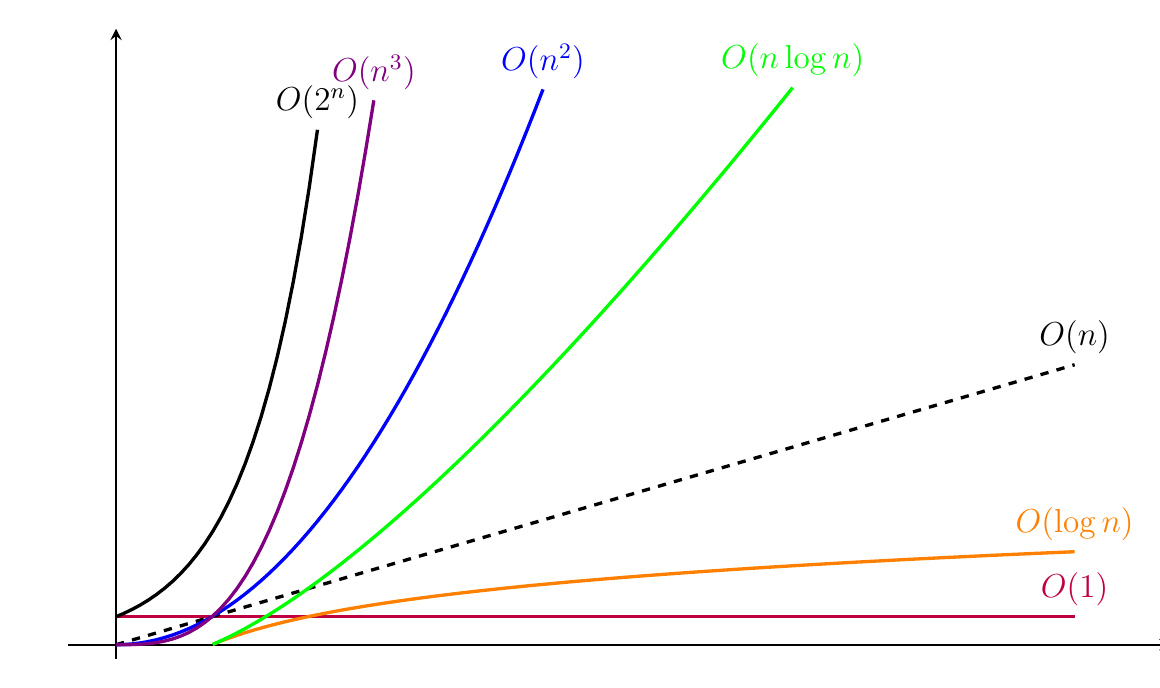
\begin{tikzpicture}[
	    mystyle/.style={above, style = {font=\large}}
	]
	    \begin{axis}[
	        % grid = major,
	        clip = true, ticks = none,
	        width = 14cm, height = 8cm,
	        enlargelimits = false,
	        scale only axis = true,
	        every axis plot/.append style = {very thick},
	        axis line style = thick,
	        clip mode = individual,
	        domain = 0:10,
	        samples = 120,  % https://stackoverflow.com/questions/59806658/how-to-draw-a-smooth-curve-in-pgfplots-and-how-to-remove-y-axis-ticks
	        no markers,
	        restrict y to domain=0:20,
	        restrict x to domain=0:10,
	        axis x line = center,
	        axis y line = center,
	        xmin = -0.5, xmax = 11,
	        ymin = -0.5, ymax = 22,
	        xlabel = {}, ylabel = {},
	        label style = {font=\large\bfseries\sffamily},
	        xlabel style = {at={(axis description cs:0.5,-0.05)}, anchor=south},
	        ylabel style = {at={(axis description cs:0.05,0.5)}, anchor=south},
	    ]
	    \addplot[color=purple] {1}                 node[mystyle]{\(O(1)\)};
	    \addplot[color=orange] {log2 x}            node[mystyle]{\(O(\log n)\)};
	    \addplot[dashed, color=black] {x}                 node[mystyle]{\(O(n)\)};
	    \addplot[color=blue] {x^2}               node[mystyle]{\(O(n^2)\)};
	    \addplot[color=green] {x*(log2 x)}        node[mystyle]{\(O(n\log n)\)};
	    \addplot[color=violet] {x^3}               node[mystyle]{\(O(n^3)\)};
	    \addplot[color=black] {2^(2*x)}               node[mystyle]{\(O(2^n)\)};    
	    %\addplot[color=factorial]    gnuplot{gamma(x+1)} node[mystyle, yshift=0.6cm]{\(\Omicron(n!)\)};
	    \end{axis}
	\end{tikzpicture}
	\caption{Several examples of asymptotic behaviours}
\end{figure}

\begin{definition} \label{TtimeTM}
Let $T$ be a function with
signature $\N \rightarrow \R^+$. We say that a Turing machine $M$ runs
in time $T$ if $M$ stops on every input $s$ after at most $T(|s|)$
steps.
\end{definition}

We also say {\em $M$ is a $T$-time Turing machine}. The algorithm
implemented by $M$ is of course $O(T)$, but the converse is not
true. (Why not?)

\begin{definition}[A polynomial algorithm]
An algorithm is {\bf polynomial} if its time complexity is $O(n^k)$
for some $k\in \N$.
\end{definition}

\begin{definition}[An exponential algorithm]
An algorithm is {\bf exponential} if its time complexity is
$O(c^n)$ for some real number $c>1$.
\end{definition}

A quick comparison shows that exponential algorithms are eventually
less efficient than polynomial algorithms. Suppose that a particular
problem can be solved by algorithm $A$ with $time_A(n)=n^5$, and also
by $B$ with $time_B(n)=2^n$. On a machine that can execute 10 million
instructions each second, $A$ solves a problem of size $n=60$ in
less than 2 minutes, while $B$ needs more than 3500 years. We say {\em
$B$ scales badly}.

It feels like it is in our interest to have polynomial algorithms for
particular problems. That is however not always possible, and even it
is, the degree of the polynomial might be too high for practical
purposes. Other (approximative/iterative) methods will need to be employed in that case: these
methods are not part of this course.



\paragraph{What if we use other types of machines?} Many other
computing formalisms are Turing-complete, so it feels a bit arbitrary
to build complexity theory starting from TMs. We will later see why it
works anyway. Another attack on TMs would be that one could express
the cost of an algorithm in terms of the number of elementary
operations needed, as for instance the comparison of swapping of two
array elements. One can read sentences like {\em quicksort is
$O(n^2)$}, but the $n$ is the number of items to sort, not the size of
the input. The $n^2$ is a (worst case) measure for the number of
comparisons, and indeed, for quicksort that is $O(n^2)$. But one
comparison takes many steps on a TM, and moreover depends on the size
of the representation of the numbers to compare. On top of that, {\em
sorting} is not a decision problem ...


\paragraph{To decide or to compute?}

A decider behaves like a function whose range has only two values:
accept and reject. On the other hand, we can interpret the contents
of the tape at the end of a decision process as the result of a
computation. If we look at it that way, the TM $M_f$ implements a
function $f$ with range $\Sigma^*$. Also, you can construct a TM $M_{fbit}$
with a tuple $\langle s,i,b \rangle$ as input -- the TM accepts if the
$i$-th bit of $f(s)$ equals $b$: $M_{fbit}$ uses $M_f$ as a {\em
subroutine}\footnote{Please make the construction more explicit}. This
shows a strong link between deciding and computing. It also works the
other way around: if you get $M_{fbit}$, you can build $M_f$ (even if
$M_{fbit}$ does not have $M_f$ inside) ... well, almost ... What is
missing?

\paragraph{Non-deterministic time complexity classes}
We later need a complexity measure for non-deterministic Turing
machines (NDTM). The non-deterministic analogue of
Definition~\ref{TtimeTM} is

\begin{definition} \label{TtimeNDTM}
Let $T$ be a function with
signature $\N \rightarrow \R^+$. We say that a non-deterministic
Turing machine $M$ runs in time $T$ if $M$ stops on every input $s$
after at most $T(|s|)$ steps for each choice of the transition.
\end{definition}


\section{Time Complexity of Languages}


Now we know about the time complexity of algorithms, we could try to
determine the {\em best} algorithm for a given language $L$. That
would give a characterization of the inherent difficulty of the
problem. That approach fails in most cases. Still, there is a way to
get some understanding of the difficulty of a problem.

\subsection{Time complexity classes}

\begin{definition}[DTIME$(T)$]
DTIME$(T)$ is the set of languages that can be decided by a
  (deterministic) $c \cdot T$-time Turing machine, with $c > 0$.
\end{definition}


$NDTIME(T)$ is similar but for a decision by a $c \cdot T$-time NDTM.

\begin{exercise}
Argue that:
\begin{itemize}
	\item If $f = O(g)$, then $DTIME(f) \subseteq DTIME(g)$.
	\item $DTIME(T) \subseteq NDTIME(T)$.
\end{itemize}
\end{exercise}

The following definition captures the class of languages that can be
decided by a polynomial Turing machine:

\begin{definition}
\P = $\cup_{k\geq 1} DTIME(n^k)$
\end{definition}

\paragraph{Examples of languages in \P}
\begin{itemize}
\item
$Sum = \{\langle a,b,c \rangle\mid a,b,c \in \N \wedge a+b=c\}$
\item
$Sorted = \{[a_1,a_2,...,a_n]\mid a_i \in \N \wedge (a_i \leq a_{i+1})\}$
\item
$Connected = \{\langle G \rangle\mid \text{$G$ is a connected graph}\}$
\end{itemize}

\paragraph{The definition of \P is robust.}
We previously committed to expressing the time complexity function on
a Turing machine with one read/write two-sided tape, and with the
possibility for the head to not move. What happens to $\P$ if we use
another machine ? The answer is ...{\em nothing} on condition we keep
it reasonable: more than one tape, one-side tape ... it does not
matter. We can even use random-access machines, n-dimensional tapes
... Each of those variant TMs can be simulated by the type of TMs we
committed to, with only a polynomial overhead. It would become tricky when
one would allow one memory cell to contain an arbitrarily large
number, or count some arithmetic operations on such numbers as unit
cost. For instance, it would be weird (but scientifically valid) to
define the time cost of the $n^{th}$ step during a T execution as
$2^{-n}$: each algorithm takes at most one time unit\footnote{This machine is known as a Zeno-machine.} ... and we can fold the
complexity theory books.


\paragraph{Outside of \P ...}
Some problems cannot be solved in polynomial time. The class of
languages that need at most exponential time contains such languages:

\begin{definition}
\EXP = $\cup_{k\geq 1} DTIME(2^{n^k})$
\end{definition}

It should be clear that $\P \subseteq \EXP$. The inclusion is even strict: see Section~\ref{timeshierarchie}.
%
The complement of \EXP is is not empty: Presburger arithmetic provides
an example.

\paragraph{How about the encoding?}
It is time to worry about the encoding of a problem, or of a language.
A decision problem is usually formulated without direct reference to
its possible encoding. For instance: we can talk about the language of
even numbers, or the problem to decide whether a number is odd or
even. Once the encoding is fixed, we can construct an algorithm, and
then perhaps determine its complexity.

For numbers, we have (at least) two natural encodings: we can use a
unary alphabet, or a binary one. In the unary one, the number $2048$
has representation length 2048, in the binary one, it has length 12. Let
us imagine a $TM_u$ and a $TM_b$ for either encoding. The best
possible $TM_u$ needs to count (modulo 2) the number of characters in
$s$, so it is $O(|s|)$. The best $TM_b$ needs to skip all characters
until it finds the last one, and then takes the decision: it is
$O(|s|)$ as well. But in terms of the size of the number represented
by $s$, the binary representation is superior: for deciding about
$2048$, $TM_b$ needs a little more than $\log_2(2048)$ steps, while
$TM_u$ needs about 2048. On the one hand, both algorithms have linear
complexity, on the other hand, the unary encoding needs exponentially
more time for deciding the same number.

A second example makes it worse: consider a naive algorithm to decide
whether a number $n$ is prime. It has a loop of the form

\begin{algorithmic}
    \State{i := 2}
    \While {$i \leq n$}
         \If{i divides n}
         \State{REJECT;}
         \EndIf
    \State{i += 1;}
    \EndWhile
    \State{ACCEPT}
\end{algorithmic}

In both encodings, the loop is executed $n$ times, but in terms of the
size of the encoding, that is exponentially less with the binary
representation than with the unary one. In one case we could think
that the algorithm is polynomial, in the other case that it is
exponential.

Clearly, we need to agree on the encoding in order to talk
unambiguously about the complexity of a problem and an algorithm. Here
is rule number one: for numbers do not use the unary encoding. You may
use binary, ternary or decimal ...: that makes no real difference
since all these representations can be transformed into each other at
only a polynomial cost. For other objects, we might have to find an
ad-hoc agreement, or sometimes, it is clear that some encodings are
bad. For graphs, we should use the adjacency matrix. Think up some
unreasonable representation for graphs, and explain why it is.


\subsection{The complexity of multiplication: an excursion}

For convenience, we use the decimal representation of numbers.
We can consider the multiplication of two numbers in the range $0..9$
as elementary. How many elementary multiplications do we need to
multiply two numbers? For simplicity, we consider numbers of the same
length (add zeros if needed):$a= a_na_{n-1}...a_1$, and
$b = b_nb_{n-1}...b_1$. We want to compute $a \times b$. At school, we
learned to do this with $n^2$ elementary multiplications, and some
additions. People have thought for a long time that it could not be
done with essentially less: the great A. Kolmogorov even put this
forward as a conjecture he strongly believed in. A. Karatsuba showed
that it was possible anyway.

Again for simplicity, assume that $n$ is even and equal to $2m$. Then
one can write $a$ and $b$ as
%
$a = A_{2}10^m + A_1$ and $b = B_{2}10^m + B_1$.
%
Then
\begin{equation*}
	a \times b = (A_{2}\times B_{2})10^{2m} + (A_{2}\times B_1 + A_1\times B_{2})10^m + A_1\times B_1
\end{equation*}
in which you can see 4 multiplications.

A. Karatsuba noticed that the coefficient of $10^m$ can be computed in
a different way:
\begin{equation*}
	(A_{2}\times B_1 + A_1\times B_{2}) = (A_{2} + A_1) \times (B_{2} +
B_1) - (A_{2}\times B_{2}) - (A_1\times B_1).
\end{equation*}
The last two multiplications give the coefficients of $10^{2m}$ and
$10^0$. By remembering the result of the last two multiplications, and
reusing it, one now gets $a \times b$ in only 3 multiplications.
By applying this principle recursively (divide and conquer) the number
of elementary multiplications is $O(n^{\log_2(3)})$. In the mean time,
algorithms with an even lower complexity have been discovered.

What did we learn from this excursion? Sometimes, intuition tells us
that there is only one possible way to compute a result, and later we
learn we were wrong: there is another (better) way, perhaps many other
ways.

\subsection{Certificates and verifiers}

The concepts of certificate and verifier are introduced here
independent of their use in complexity: you must be able to understand
and interpret their definitions (and properties) without referring to
complexity.

\begin{definition} \label{verifiercertificate}
A {\bf verifier} for a language $L$ is a deterministic TM $V$
such that

~~~~~~~~~~~~~~~~~~~~~~
$\forall s \in \Sigma^* : (s \in L \leftrightarrow \exists c \in \Sigma^*: V(\langle s,c \rangle) = accept)$

$c$ is named a {\bf certificate} for $s$.
\end{definition}

\begin{example}
Some examples of certificates and verifiers:
\begin{itemize}
\item Let $L$ be the set of composite numbers. There exists of course a TM
$M$ that decides that language: a typical algorithm would try to find
a divisor for a given number. However, if a number $n \in L$ then
there exists a divisor $d$, and we could give the numbers $n$ and $d$
to a TM $V$ that verifies that $d$ is indeed a divisor of $n$: $V$
has less work to do than $M$, and according to the definition, it is a
verifier for $L$, while the given divisor $d$ is the certificate. Note
that it impossible to fool or mislead the verifier: you cannot make it
accept a prime as a composite.

\item
Let $L$ be the language of tuples of the form $\langle G,a,b \rangle$
in which $G$ is a graph, and $a$ and $b$ are vertices connected by a
path in $G$. Once more, there exists a TM $M$ that decides exactly
this language, by just trying to construct a path. A verifier $V$ can
be easier: a possible certificate is a path between $a$ and $b$. $V$
merely needs to check that this certificate is really a path in $G$,
starting with $a$ and ending with $b$. Verifying something is a path
is easier than constructing it: $V$ needs less work than $M$. Try to
fool $V$ ... It is impossible.

\item
Let $L$ be the set of TMs $M$ for which $L_M$ is not empty. We showed
earlier that this language is not decidable. Still, for every TM $M$
with $L_M \neq \emptyset$, there is a certificate that it is in $L$,
namely any $c \in L_M$. The verifier just runs $M$ on $c$

\end{itemize}
\end{example}

The first two examples give the intuition that the job of a verifier
for $L$ is easier than the job of a decider for $L$. The last example
makes it blatantly clear: the language does not need to be decidable
in order to have a verifier/certificate.

Confused? Think about it, reread Definition~\ref{verifiercertificate}.

It might have escaped your attention:
Definition~\ref{verifiercertificate} does not mention strings that do
{\bf not} belong to the language. You get to know something about such
strings by juxtaposition. You get: for $s \notin L$, every $c$ is {\bf
not} a certificate.

Think about this: the definition of verifier/certificate says nothing
about strings {\bf not} in the language.

The intuition holds up: a verifier must work less than a decider. Some
questions remain:
\begin{itemize}
\item
does every language have a verifier and a certificate for each string
in the language?
\item
can a string have more than one certificate?
\item
how difficult is it to construct (by an algorithm) a certificate? is
that always possible?
\end{itemize}

The second question above has {\em yes} as answer for each of the
three examples: every divisor is a certificate for a composite number.
Every path is a certificate for the fact that $a$ and $b$ are
connected. Every $s \in L_M$ is a certificate.

As for the last question: for the first two examples, the certificate
can be generated by an algorithm (although nobody knows whether it can
be done in polynomial time in the first example); in the third
example, no algorithm can generate a certificate for each
string. Think about this: it might be a bit more subtle than you think
at first.

\begin{exercise}
An additional question can be asked about the length of the certificate: is there a relation between the length of $s \in L$ and the length of its certificate, and the complexity (or decidability) class of $L$?

Consider all three examples and comment on that question.
\end{exercise}
Suppose there is a function $f$ so that for a verifier $V$ and
certificate $c$ for $s$, the length of $c$ has an upper bound of
$f(|s|)$, or:
%
$|c| \leq f(|s|)$. Now we can generate a certificate for
any $s \in L$ as follows:

\begin{algorithmic}
    \ForAll {$(i \leq f(|s|) \wedge (c \in \Sigma^i)$}
         \If {$V(\langle s,c \rangle)$ accepts}
         \State{ACCEPT}
         \EndIf
    \EndFor
    \State{REJECT}
\end{algorithmic}

This deterministic algorithm\footnote{Is it an algorithm or can you
turn it into one?} tries all potential certificate candidates. Can we
say something about its complexity?


\begin{itemize}
\item
in the worst case, the for-loop is executed $O(2^{f(|s|)})$ times (we assume
the alphabet has two elements)
\item
if $V$ is a $g$-time machine, the cost of the body of the for-loop is
$O(g(|s|+|c|))$, or $O(g(|s|+f(|s|)))$
\item
this results in an overall complexity $O(g(n+f(n))\times 2^{f(n)})$
where $n$ is the size of the input
\end{itemize}

If $f$ and $g$ are at least linear, the complexity of this algorithm
is exponential or worse, even if $g$ is not. You might feel like
arguing that for some problems there is a less naive way to generate
certificates (think about the connected vertices), and you are right
... but there are quite a lot of problems for which science has not
achieved that. We will see more about this later.

The algorithm above {\em guesses systematically} for a
certificate. One can model that with a non-deterministic procedure,
e.g.\ by a Prolog predicate. It can also be modelled with a
non-deterministic Turing machine {\em NDTM$_V$} with just two
transitions at each stage. On input $s$, {\em NDTM$_V$} writes in its
first $f(|s|)$ steps non-deterministically a string from
$\Sigma^{f(|s|)}$ on the tape. It then calls the deterministic
verifier $V$. If one of the branches accepts, $s$ is accepted.
Figure~\ref{nondetverifier} illustrates this: the length of the
certificate is 2.


\begin{figure}[h]
	\centering
	\includegraphics[height=0.2\textheight,keepaspectratio]{nondetverifier}
	\caption{Generation of a certificate when the length is
	known}\label{nondetverifier}
\end{figure}

Vice versa, we can transform this {\em NDTM$_V$} into a verifier: it
needs a certificate. Give as certificate a string representing the
choices needed for arriving at an accepting state. Now simulate
{\em NDTM$_V$} with those choices, of course with a deterministic TM
...

We have just (informally) shown that one can go back and forth between
a verifier+certificate (with known length) and a non-deterministic
Turing machine.



\subsection{Two definitions of \NP}

The class \NP can be defined in two ways: the material in the previous
section contains the ingredients to prove their equivalence.

\begin{definition}[\NP with verifiers]
\NP is the set of languages $L$ for which there exists a polynomial
verifier and a polynomial $p$ such that for each $s \in L$, there
exists a certificate $c$ so that $|c| \leq p(|s|)$.  ~\\ ~\\
More formally: $L \in \NP$ if and only if

$~~~~~~~~\exists$ a polynomial TM $M$ and a polynomial $p: \N
\rightarrow \R^+$, so that

$~~~~~~~~~~~~~~~s \in L  \Leftrightarrow  \exists c \in \Sigma^{p(|s|)}$ with $M(\langle s,c \rangle) = accept$
\end{definition}

The alternative definition of \NP uses non-deterministic Turing machines:

\begin{definition}[\NP with non-determinism]
\NP is the set of languages decided by a polynomial non-deterministic
Turing machine.
\end{definition}

You should be able to argue that these two definitions define the same
set. Also, you must be able to argue that \NP is robust with respect
to the execution model.

{\bf Careful:} \NP means {\em non-deterministic polynomial},
and {\bf not} {\em non-polynomial}.

\begin{example}
Some examples of languages in $\NP$:

\begin{itemize}
\item
since $\P \subseteq \NP$ (why?) each language in \P can serve as an example ...
\item
pairs of isomorphic graphs (*)
\item
graphs with a Hamiltonian cycle (*)
\item
non-connected graphs
\item
weighted graphs with a simple path shorter than
a given number between two given nodes (*)
\item
Come up with something yourself!
\end{itemize}
Note that for the examples marked with (*), no polynomial
algorithm is known, neither whether one exists.
\end{example}

\begin{exercise}
Give for each example a description of a verifier and a certificate
for a string belonging to the language. Argue that it is
polynomial.
\end{exercise}

\subsection{Polynomial reduction}

In a previous chapter, we have reduced languages to each other: the
many-one reduction $\leq_m$ {\mbox is an example} (see
page~\pageref{manyone}). The reduction below takes
complexity into account.

\begin{definition}[Polynomial reduction]
Given two languages $L_1\subseteq \Sigma_1^*$ (over alphabet $T_1$)
and $L_2\subseteq \Sigma_2^*$ (over $T_2$). We say that $L_1$
reduces polynomially to $L_2$ if there exists a mapping $f:\Sigma_1^*
\rightarrow \Sigma_2^*$ so that:
\begin{verse}
1. $\forall x\in \Sigma_1^*$: \ \ \ $x\in L_1\Leftrightarrow f(x)\in
L_2$\\[2mm] 2. There exists a deterministic TM that computes $f$ in
polynomial time.
\end{verse}
We denote this by $L_1 \leq_p  L_2$.
\end{definition}

$\leq_p$ differs from $\leq_m$ only in the fact that the mapping must
be computable in polynomial time. This makes $\leq_p$ finer than $\leq_m$:
if $A \leq_p B$ then $A \leq_m B$. Check whether some of the examples
of $\leq_m$ earlier in this course notes were actually $\leq_p$?

\begin{theorem} \label{transitief}
The relation $ \leq_p $ is transitive, or more explicitly:\\
if $L_1 \leq_p L_2$ and $L_2 \leq_p L_3$ then $L_1 \leq_p L_3$.
\end{theorem}
\begin{proof}
Let $f$ be the polynomial computable function belonging to $L_1
\leq_p L_2$, and $g$ to $L_2 \leq_p L_3$. $M_f$ and $M_g$ are the
corresponding TMs: the first is a $T_f$-machine, the second a
$T_g$-machine, and $T_f$ and $T_g$ are polynomials. We prove that
%
the function $h = g\circ f$ is good for $L_1 \leq_p L_3$.

Clearly, $s \in L_1 \Leftrightarrow h(s) \in L_3$, and $h$ is
computable by a TM $M_h$: first let $M_f$ run on $s$, and when it is
finished, move the head to the left, and then let $M_g$. We just need
to show that $M_h$ is polynomial.

Let $s$ be a string with {\em a large enough} length be the input for
$M_h$. When $M_f$ is finished, the tape contains a string $s_f$ with
length at most $T_f(|s|)$. So, moving the head to the left costs at
most a polynomial (in $|s|$) amount of work. Executing $M_g$ on $s_f$
takes at most $T_g(T_f(|s|)$ time, so together we have as an upper
bound for the total time of $M_h$:
%
$T_f(|s|) + T_f(|s|) + (T_g \circ T_f)(|s|)$ which is polynomial in
$|s|$.
\end{proof}


The next theorem has the same feel as an earlier theorem about
$\leq_m$.

\begin{theorem} \label{P_is_klein}
If $L_1  \leq_p  L_2$ and $L_2\in \P$ then $L_1 \in \P$.
\end{theorem}
\begin{proof} Let $L_1\subseteq \Sigma_1^*$, $L_2\subseteq \Sigma_2^*$, and $L_1
\leq_p L_2$ via the function $f: \Sigma_1^*\rightarrow \Sigma_2^*$ that is
polynomially computable by TM $M_f$. Since $L_2\in \P$, there exists a
TM $M_2$ that decides $L_2$ in polynomial time. Construct TM $M$: it
executes $M_f$ and $M_2$ in sequence. Just as in the previous theorem,
we can prove that $M$ has polynomial time complexity. Moreover, $M$
decides $L_1$, so $L_1\in \P$.
\end{proof}

We name two languages equivalent if each can be polynomially reduced
to the other.

\begin{definition}[Polynomial equivalence of languages]
Two languages $L_1$ and $L_2$ are polynomial equivalent (denoted by
$L_1\sim_p L_2$) if
\[ L_1 \leq_p  L_2 \mbox{ \ and \ } L_2  \leq_p  L_1\]
\end{definition}


The wording in this definition is justified by

\begin{theorem}
The relation $\sim_p$ is an equivalence relation.
\end{theorem}
\begin{proof} We need to show that $\sim_p$ is reflexive, symmetric
and transitive. Reflexivity is trivial, symmetry follows directly from
the definition of $\sim_p$, and transitivity was already proven in
Theorem~\ref{transitief}.
\end{proof}

As with any equivalence relation, we can consider the equivalence
classes induced by the relation. They form a partition. \P consists
of exactly three equivalence classes.

\begin{theorem}
	$\sim_p$ partitions \P into the equivalence classes $\{\emptyset\}$, $\{\Sigma^*\}$ and $\P \setminus \{\emptyset, \Sigma^*\}$.
\end{theorem}
\begin{proof}
Consider two languages $L_1,L_2\in \P \setminus \{\emptyset, \Sigma^*\}$. To prove $L_1 \leq_p L_2$ and vice versa, we need a mapping reduction that maps all strings $x\in L_1$ to a string in $L_2$ and all strings $x\notin L_1$ to a string outside of $L_2$, and which finds these mappings with a time complexity polynomial in $|x|$.

Verifying whether a string is in or out of $L_2$ takes polynomial time in the size of the verified string, but constant time in $|x|$. Enumerating strings in $\Sigma_2^*$ is also independent of the size of $x$, so it too is constant-time in $|x|$. Hence, we can search for a string $a \in L_2$ and a string $b \notin L_2$ for free!

A polynomial mapping $f(x)$ from $L_1$ to $L_2$ is then simply:
\begin{equation*}
	f(x) = \begin{dcases}
		a &\quad(x\in L_1)\\
		b &\quad(x\notin L_1)
	\end{dcases}
\end{equation*}
... since the check $x\in L_1$ takes polynomial time in $|x|$ and finding $a$ and $b$ is independent of the size of $x$. Hence, $\P \setminus \{\emptyset, \Sigma^*\}$ is entirely part of one equivalence class.

Do $a$ and $b$ always exist? Yes, except in two languages: $L = \emptyset$ has no $a$, and $L = \Sigma^*$ has no $b$. The above $f$ is only one approach to the reduction, but it's easy to see how the lack of $a$ or $b$ plagues every reduction, except from $\emptyset$ to itself and $\Sigma^*$ to itself. This means $\{\emptyset\}$ and $\{\Sigma^*\}$ are two separate (singleton) equivalence classes of $\P$, and that no other languages are missing in the equivalence class we started above for the rest of $\P$.
\end{proof}

\subsection{NP--complete}
Within $\NP$, there exists a special class of languages: the most
difficult of all in $\NP$!

\begin{definition}[The class $\NP$--complete] \label{defnpc}
	A language $L$ is $\NP$--complete iff
	\begin{enumerate}
		\item $L\in \NP$ and
		\item for each language $L'\in\NP$, it is true that $L' \leq_p  L$.
	\end{enumerate}
	We denote the class of $\NP$--complete languages by $\NPC$.
\end{definition}

Informally, an $\NP$--complete language is so difficult that any other
language can be translated to it in polynomial time. In terms of problems:
a problem is $\NP$--complete if it has a solution (in the form of an
algorithm) so that every other $\NP$ problem has a solution that can
be deduced from the $\NP$--complete solution by a polynomial reduction. 

A language $L$ that fulfills at least the second condition of Definition
\ref{defnpc} is named {\em $\NP$--hard}. (One also uses $\NP$--hard for
optimization problems whose decision version is $\NP$--complete.)

A priori, it is not clear whether
$\NP$--complete or $\NP$--hard languages exist at all, neither whether $\NPC$
coincides with $\NP$ or $\P$. The first is easy to solve: all the undecidable problems of past chapters belong to $\NPhard$ and not to $\NP$. The relevance of $\NPC$ is captured in the following theorem:

\begin{theorem}~
	\begin{enumerate}
		\item \NPC is an equivalence class for $\sim_p$.
		\item If $\NPC\cap\P\neq \emptyset$ then $\NP=\P$.
	\end{enumerate}
\end{theorem}
\begin{proof*}
\begin{enumerate}
	\item Suppose $L_1,L_2\in\NPC$. By the definition of $\NP$--completeness,
	both $L_1 \leq_p L_2$ and $L_2 \leq_p L_1$. So, $L_1$ and $L_2$ are
	polynomially equivalent. The class $\NPC$ is therefore part of one
	equivalence class $C$. Are there other languages in $C$? Suppose that $L_* \in C\setminus \NPC$. For all $L\in\NPC$, the equivalence $L\sim_p L'$ holds by definition of $C$, so two things are true: 
	\begin{enumerate}
		\item $L \leq_p L_*$: by transitivity with the rest of $\NP$, $L_* \in\NPhard$;
		\item $L_* \leq_p L$: this means $L_*$ can be solved in $\NPC$ complexity (after negligible polynomial overhead), meaning that $L_*\in\NP$ (and not $L_*\in\NPhard\setminus\NPC$).
	\end{enumerate}
	Thus $C = \NPC$.
	
	\item Suppose $L\in\P \cap\NPC$. Consider any other language $L'\in
	\NP$. Since $L\in\NPC$, we know that $L' \leq_p L$. Since also
	$L\in\P$, it follows from Theorem~\ref{P_is_klein} that $L'\in
	\P$. So, $\NP=\P$.\vspace{-2em}
\end{enumerate}
\end{proof*}

The previous theorem shows that if one $\NP$--complete
problem can be solved in polynomial time, all problems in \NP can be
solved in polynomial time. There is however lots of evidence that \NP
does not equal $\P$.\footnote{On the other hand ... Donald Knuth
believes in $\P = \NP$.}

Figure~\ref{NP-venn} shows the two possibilities: either $\P \neq \NP$
or $\P = \NP$.

\begin{figure}[ht]
	\centering
	\includegraphics[width=0.7\linewidth,keepaspectratio]{NP-venn}
	\caption{The possible relation between $\P$, $\NP$ and $\NPC$
	 \label{NP-venn}}
\end{figure}
The set $\NP$-intermediate is not empty if $\P \neq \NP$. A candidate
$\NP$-intermediate problem is {\em graph isomorphism}.

The first problem proven to be in \NPC is the {\em satisfiability}
problem, often abbreviated by SAT. We need some definitions to specify
the SAT language. Let $U = \{u_1,u_2,\ldots,u_n\}$ a finite set of
boolean variables, i.e.\ each variable $u_i$ can take the values {\em
true} or {\em false}.  By a literal (or an atom) from $U$ we mean either one
of the variables $u_i$, or its negation denoted by $\neg {u}_i$ (read
this as {\em not $u_i$}). Consider a formula in Conjunctive Normal
Form (CNF) over $U$, i.e.\ a conjunction of disjunctions of literals
over $U$ as in the following example:
%
$C= (u_1 \vee u_2) \wedge (u_2 \vee \neg u_4 \vee u_7) \wedge  (\neg u_2 \vee u_3)$.

The SAT problem is: given a formula in CNF, does there exist a truth
assignment to the variables so that the formula is true?

More precisely, SAT is the language of CNF formulas that have a
satisfying assignment.

Stephen A. Cook\footnote{Turing award 1982} proved in 1971

\begin{theorem}[The Cook-Levin Theorem]
$SAT \in \NPC$
\end{theorem}

We do not study the proof of this theorem in this course. What you
should be able to do is: show that $SAT \in \NP$, once using the
non-deterministic definition of $\NP$, and once using the verifier
definition. What is the size of the certificate? How did you encode
the language?

Once the first $\NP$--complete problem was known, many more
were found.
\begin{example}
A few languages/problems in $\NPC$: Hamiltonian
graphs, N-colorable graphs, subgraph isomorphism, the knapsack
problem, pancake sorting, 0-1 integer programming, lots of
combinatorial problems and even puzzles like Sudoku.
\end{example}

\begin{exercise}
$SAT$ has a polynomial reduction to $H_{TM}$,
and so does every other problem in $\NP$. Work this one out!
\end{exercise}


\subsection{Examples of polynomial reductions}

\subsubsection{SAT to 3-SAT}

3-SAT is SAT with the restriction that each disjunction in the CNF has
exactly three literals. One formula in 3-SAT is
%
$(a \vee b \vee \neg c) \wedge (\neg a \vee b \vee c)$.

\begin{theorem}[SAT to 3-SAT]
Every propositional formula in CNF can be transformed to CNF with 3 literals per disjunction.
\end{theorem}
\begin{proof}
Consider each disjunction in the formula. There are three cases:
\begin{enumerate}
\item
the disjunction contains fewer than three literals: repeat one of the
literals until there are three
\item
the disjunction contains exactly three literals: just leave them
unchanged
\item
the disjunction contains strictly more than three literals: the
disjunction is of the form
%
$a_1 \vee a_2 \vee  ... \vee a_n$ with $n > 3$.

Take a new boolean variable, say $b$, and replace this one disjunction
by the two disjunctions
\begin{equation*}
	\left\{\begin{aligned}
		b &\vee a_{n-1} \vee a_n \\
		\neg b &\vee a_1 \vee a_2 \vee  ... \vee a_{n-2}
	\end{aligned}\right.
\end{equation*}

Repeat all this until no disjunction contains more than three literals.\vspace{-1.75em}
\end{enumerate}
\end{proof}

This brings us one step closer to proving that 3-SAT is in $\NPC$: a formula $\in SAT$ is mapped to a formula $ \in$ 3-SAT, and a string $\notin SAT$ is mapped to a string $ \notin$ 3-SAT. Furthermore, this transformation can be implemented on a polynomial TM. Hence, 3-SAT is at least as hard as SAT: it is in $\NPhard$.

Members of 3-SAT also have a polynomial certificate (and a verifier like SAT), so 3-SAT $\in \NP$. In that case, 3-SAT $\in (\NP \cap \NPhard) = \NPC$.


You should now be able to show that $n$-SAT $\in \NPC$ whenever $n \geq 3$, but ... 2-SAT has a polynomial algorithm in the number of occurring
literals. It works something like this: any 2-SAT clause $a \vee b$ is equivalent to $\neg(\neg a)\vee b$ which is just $\neg a \Rightarrow b$. The CNF is a collection of these rules. Now make chains of implications: if you derive $a \Rightarrow \hdots \Rightarrow \neg a$, the CNF is unsatisfiable. One can even find in the literature that 2-SAT has a
linear algorithm, but that is on a random access machine, not on a
TM. In any case, 2-$SAT \notin \NPC$ (although ``not being in $\NPC$'' always has the caveat that $\P \neq \NP$).


\subsubsection{Reducing 3-SAT to $k$-CLIQUE}

The language $k$-CLIQUE consists of tuples $\langle G,i \rangle$
in which $G$ is a graph with a clique of size $i$, or otherwise said:
$G$ contains a subgraph isomorphic to $K_i$. Two examples show how the
reduction works:

\begin{figure}[h]
	\centering
	\includegraphics[height=0.2\textheight,keepaspectratio]{satclique}
	~~~~~~~~~\includegraphics[height=0.2\textheight,keepaspectratio]{satcliquesol}
	\caption{The graph corresponding to the first formula, and a
	4-clique}\label{satclique}
\end{figure}

\begin{example}
The formula in 3-SAT is

$(a \vee b \vee c) \wedge (a \vee \neg b \vee \neg c) \wedge (\neg a \vee b \vee \neg c) \wedge (\neg a \vee \neg b \vee c)$

Figure~\ref{satclique} shows at the left the graph resulting from the
reduction:
\begin{itemize}
	\item each occurrence of a literal corresponds to one vertex with as its name the literal. Note: this likely causes vertices with the same name; we tolerate this. 
	\item there is an edge between two vertices that are {\em compatible}: $p$
	and $\neg p$ are not compatible and two vertices (\emph{not} labels!) from the same
	disjunction are not compatible either.
\end{itemize}
The incidence matrix of this graph can be computed in polynomial
time. The required clique size (4 in the example) is the number of
disjunctions in the formula.
\end{example}

Convince yourself that the graph has a clique of the required size if
and only of the formula belongs to SAT.

\begin{figure}[h]
	\centering
	\includegraphics[height=0.2\textheight,keepaspectratio]{satclique2}
	\caption{The graph corresponding to the second formula: there is no 4-clique}\label{satclique2}
\end{figure}

\begin{example}
The reduction can be applied to smaller disjunctions as well. We take the following
as the formula: $(a \vee b) \wedge (\neg a \vee b) \wedge (a \vee \neg b)
\wedge (\neg a \vee \neg b)$.

Because the graph has no 4-clique, the formula does not belong to
SAT. Of course, the graph does have $k$-cliques: the maximal $k$ gives us
the maximal number of disjunctions that can be true at the same
time. In this way, two optimization problems are connected by a
polynomial reduction.

\end{example}

\begin{exercise}
On the topic of the above reduction:
\begin{itemize}
\item Do you see a correspondence between the reduction from SAT to 3-SAT
and how we put a CFG into Chomsky Normal Form?

\item Reduce $3$-SAT to SAT.
\end{itemize}
\end{exercise}

\begin{exercise}
We can generalise the previous question:

\begin{itemize}
\item Does $A \subseteq B$ and $A \in \P$ imply that $B \in \P$?

\item Does $A \subseteq B$ and $A \in \NP$ imply that $B \in \NP$?

\item Does $A \subseteq B$ and $A \in \NPC$ imply that $B \in \NPC$?

\item Does $A \subseteq B$ and $B \in \P$ imply that $A \in \P$?

\item Does $A \subseteq B$ and $B \in \NP$ imply that $A \in \NP$?

\item Does $A \subseteq B$ and $B \in \NPC$ imply that $A \in \NPC$?

\end{itemize}

\end{exercise}

\subsection{Why are some problems difficult?}

For SAT, one could argue as follows: there are $2^n$ possible
assignments ($n$ is the number of boolean variables), and our
intuition tells us that we need to check all of them to find the good
one (or on average half of them) ...

For Hamiltonian cycles, we would argue: the number of simple cycles in
a graph is exponential in the number of vertices, and our intuition
tells us ...


For MSTs, we would argue: the number of spanning
trees for a graph with $n$ vertices can be at worst $n^{n-2}$ -- that
is even worse than exponential, so our intuition ... would be totally
wrong. Indeed, we saw a greedy polynomial algorithm for this
problem: Prim and Kruskal. We relied on a graph theorem
that guaranteed the correctness of a polynomial algorithm without the
need to check all possibilities.

Perhaps we have not yet proven the right theorem for SAT, the
theorem that results in a polynomial algorithm for SAT, but if we do,
we will need to adjust our intuition just as with Karatsuba and
multiplication.

\section{The Time Hierarchy}\label{timeshierarchie}

As far as we discussed it, the structure of \P is rather uniform.
The time hierarchy theorem changes that: below is a correct version,
but not the strongest possible one:

\begin{theorem}
$DTIME(f) \subsetneq DTIME(f^2)$ for every {\em time-constructible}
$f$.
\end{theorem}

Loosely speaking, a function $f$ is time-constructible if $f$ can be
computed on a TM in $O(f)$ steps and $f(n) \geq n$. Most probably, you
will never during your life meet a (non-trivial)
non-time-constructible function :-)  % [NOTE TB] What about log(n)?

R. Stearns and J. Hartmanis proved the first version of the
time hierarchy theorem in 1965, quite a few years before the notion of
$\NP$--completeness came to life. For that - and other things - they
got the Turing award in 1993.

It is important to realize that strictly more problems can be solved
with a $O(n^4)$ algorithm than with $O(n^2)$: time is a resource, and
it is limited.
\begin{exercise}
This is a good moment to think about the following:
\begin{itemize}
	\item How many languages are in $DTIME(n^k)$?
	
	\item How many languages are in $\P$?
	
	\item How many languages are in $\NP$?
	
	\item If you answered {\em countably infinite} to one or more of these
	questions, would that also be effectively enumerable?
\end{itemize}
\end{exercise}


\section{co-\NP}

Since the definition of \NP treats elements of the language
differently from the ones not in the language, it is worthwhile
investigating the complement of languages in $\NP$:

\begin{definition}[co-\NP]
co-\NP = $\{L \mid \overline{L} \in \NP\}$
\end{definition}

Be careful: co-\NP does not equal $\overline{\NP}$. The latter
contains non-decidable languages like $A_{TM}$, but every language in
co-\NP is decidable (why?).

\begin{example}
Some examples provide the intuition that co-\NP might be different from $\NP$.
\begin{itemize}
\item $SAT \in \NP$ because we have a short (polynomial) certificate for
satisfiable formulas. $\overline{SAT} \in co$-$\NP$. How about
certificates for elements in $\overline{SAT}$? $\overline{SAT}$
contains the formulas for which no assignment is satisfying ... Could
that have a short certificate? Nobody knows.

\item Consider $TAUTOLOGY$. It is the language of formulas that are true
for {\bf every} assignment to the variables. $\overline{TAUTOLOGY}$
is definitely in $\NP$: a short certificate would be an assignment
that makes the formula false, but a short certificate that can be
verified in polynomial time to show the formula is a tautology
... Nobody knows.

\item The set of sorted sequences is a language in $\NP$. A certificate
for a non-sorted sequence would be an index $i$ so that the i$^{th}$
element is larger than the (i+1)$^{th}$ element. So the set of sorted
sequences belongs to co-$\NP$ as well. You could have argued: the set
of sorted sequences is in $\P$, so also in co-$\NP$. That is right, but
you would have missed thinking up a non-trivial polynomial certificate.

\item $COMPOSITE$ (the set of composite numbers) has a short certificate: a
divisor of the number. It is difficult to think of a short
certificate for PRIME (which is $\overline{COMPOSITE}$). On the other
hand, since 2004 we know that PRIME $\in \P$, so this short
certificate indeed exists ... Can you think of one?
\end{itemize}
\end{example}
After these examples, you should understand that $\P \subseteq \NP
~\cap$ co-$\NP$, and that $\NP = $ co-\NP is not a trivial question. You
must also be able to argue that $\P = \NP$ implies $\NP = $ co-$\NP$.
And what if $SAT \in$ co-$\NP$?

\section{$\NP$--complete or $\P$?}

In this section, we merely want to point out that the details of how a
problem is specified really matter. Consider the following two
languages:

\begin{verse}
- $k$-CLIQUE $= \{\langle G,i \rangle\mid \text{$i$ an integer, $G$ a graph with an $i$-clique}\}$

- 7-CLIQUE $= \{\langle G \rangle\mid \text{$G$ a graph with a 7-clique}\}$
\end{verse}

We showed that $k$-CLIQUE is in \NPC (we reduced SAT to it), but
7-CLIQUE is polynomial: let $n$ be the number of vertices in $G$. There
are $C_n^7$ subsets of vertices that potentially form a
7-clique. Checking one of them is polynomial in the size of $G$, say
$O(n^c)$ for some $c$. Moreover,
\begin{equation*}
	C_n^7 = \frac{n!}{(n-7)!\, 7!} = \frac{n(n-1)\hdots(n-6)}{7!} = O(n^7)
\end{equation*}
so we have a naive
algorithm with time complexity $O(n^{c+7})$. The encoding of $G$ has
size $O(n^2)$, so the 7-CLIQUE is in $\P$.

This phenomenon shows up quite often: by keeping one or more
parameters of the problem constant, we get a polynomial version of an
$\NP$-complete problem.

Reconsider the following two problems:

\begin{verse}
- $A_{TM} = \{\langle M,w \rangle \mid w \in L_M\}$

- $E_{TM} = \{\langle M \rangle \mid \epsilon \in L_M\}$
\end{verse}

By keeping one parameter in $A_{TM}$ fixed, we get $E_{TM}$. Did that
pay off in this case?



\section{Space Complexity}

Space is a resource: has your Java program ever stopped unexpectedly
because of stack overflow? Or has the progress of your program ever
become unacceptably slow because of excessive swapping or garbage
collection? If so, you know that space is a (limited) resource, and
space complexity deals with it. One could try to define the space
complexity of an algorithm (on a TM) as the number of cells that are
read/written on the tape. That would not be so useful:
\begin{itemize}
\item for non-trivial problems, the input needs to be read completely, so
space complexity could not be sublinear: the space cost of the input
is indeed unavoidable

\item on the other hand, many algorithms need very little {\em
extra} space (besides the input)
\end{itemize}

The latter should be familiar. E.g. testing whether a sequence is
sorted needs an index and a fixed amount of space for comparing the
two consecutive cells in the sequence: a constant space overhead.

Before we start with the definitions, think about this: one can reuse
space, one cannot reuse time! So one expects to need {\em less} space
than time for solving a given problem.

The definition of space complexity is based on a Turing machine model
with
\begin{enumerate}
\item one read-only tape containing the input string

\item one read-write tape
\end{enumerate}
The space cost of an algorithm is equal to the number of cells used on
the R/W tape.

\begin{definition}
DSPACE(f) is the set of languages decided by a deterministic Turing
machine using $O(f)$ cells on the R/W-tape.
\end{definition}

\begin{lemma} \label{grootte_van_string}
If the function $f$ is computed on a $T$-time TM, then
%
$|f(s)| \leq T(|s|)$.
\end{lemma}
This essentially says that a TM cannot write on more tape cells than
it makes steps.

Now, you argue that $DTIME(f) \subseteq DSPACE(f)$.

\begin{definition}
$\PSPACE = \cup_{k\geq 1} DSPACE(n^k)$
\end{definition}

It should be clear now that $\P \subseteq \PSPACE$.

Just as for time, there exists a space hierarchy
theorem. E.g. $DSPACE(f) \subsetneq DSPACE(f^2)$ for {\em decent} $f$.

\begin{definition}
$\NPSPACE$ is like $\PSPACE$, but with non-deterministic Turing
  machines.
\end{definition}

The inclusion $\PSPACE \subseteq \NPSPACE$ is easy to prove, and one
might suspect that $\PSPACE \neq \NPSPACE$, or that it is unknown.
Surprise ... $\PSPACE = \NPSPACE =$ co-$\NPSPACE$. The fact that
non-determinism does not change $\PSPACE$ is related to the fact that
space can be reused: a non-deterministic TM can be simulated
deterministically with little space overhead. That provides the
intuition that co-$\NPSPACE$ must equal $\NPSPACE$.


\paragraph{Less than linear space?} This is also possible. Consider the
language of even numbers: one can decide it with no extra space at all!
This works actually for all regular languages. There exist also
languages beyond RegLan that can be decided in sublinear space. As an
example, we consider the problem to decide whether there exists a path
between two given vertices in a given directed graph $(V,E)$. We
describe (in pseudo-code) a $\log(n)^2$-space algorithm: $n$ is the
number of vertices.

\begin{algorithmic}
\Function {existspath}{a,z,l}
\If {$(l = 0)$}
\State{return(a = z)}
\EndIf
\If {$(a,z) \in E$}
\State{return(TRUE)}
\EndIf


\ForAll {$(v \in V)$}
   \If {{\sc existspath}$(a,v,l/2)~ \wedge~ ${\sc existspath}$(v,b,l-l/2)$}
   \State{return(TRUE)}
   \EndIf
\EndFor
\State{return(FALSE)}
\EndFunction
\end{algorithmic}

{\sc existspath}$(a,z,n)$ returns TRUE if there exists a path from a
to z with length at most l. Its time complexity is horrible. If you
imagine it is executed on a classical machine (your laptop), you see
that no more than $\log(n)$ stack frames are needed, and that each
stack frame has size at most $\log(n)$ bits. The algorithm can be
implemented on a DTM with the same space complexity.

It is also interesting that one can trade space for time: you can make
a version of \mbox{{\sc existspath}} that uses less time, but more
space, e.g.\ by using a depth-first backtracking search through the
graph, while you remember the visited nodes: that is $O(n)$.

Algorithms (and problems requiring them) that use log-space are
interesting enough to warrant their own class:

\begin{definition}
$\LL = DSPACE(\log)$
\end{definition}


Log-space algorithms are important, e.g.\ in the context of large
databases, or long DNA-sequences: with the log of the space taken by a
database, you can keep a fixed number of pointers (in binary) and
that is often enough to traverse the database and answer queries.

\section{Discussion}
\subsection{Informal class definitions}
It's useful to know single-sentence summaries of the big time complexity classes we saw.
\begin{itemize}
	\item $\P$: decidable in polynomial time w.r.t.\ input size.
	\item $\NP$: decidable by verifying a polynomial-sized certificate in polynomial time, both w.r.t.\ input size.
	\item $\NPC$: most complex languages in $\NP$.
	\item $\NPhard$: languages at least as complex as the most complex languages in $\NP$.
\end{itemize}
Other terminology exists: ``deciding a language'' is often cited as ``solving a problem'', and ``complex'' becomes ``hard/difficult/expensive''.

On a Venn diagram, all of these are drawn as their own ellipse (see), except for $\NPC$, which is the \emph{intersection area between} two (or more?) circles.

\subsection{A sequence of inclusions}
We know enough at this point to justify the following
sequence of inclusions:

\begin{verse}
$\LL \subseteq \NL \subseteq \P \subseteq \NP \subseteq \PSPACE
  = \NPSPACE \subseteq \EXP$
\end{verse}

Thanks to the hierarchy theorems, we know for sure that
$\LL \neq \PSPACE$ and $\P \neq \EXP$. This means that some of the
inclusions are strict, but currently nobody knows which ones.


\subsection{Complexity and Chomsky hierarchy}

What is the connection between the complexity of a language and its
place in the Chomsky hierarchy?

It is easy to see that a regular language can be decided in $O(n)$
steps if $n = |s|$ on an FSA, and this stays the same if used as the brain of a TM.
One needs very little extra space to
decide a regular language, actually none at all. Besides, only regular
languages can be decided with strictly less than $\log$-SPACE.

Context free languages can be recognized by a general $O(n^3)$
algorithm (on a 3-tape TM) known by the names of the authors
as Cocke-Younger-Kasami. It is a form of {\em chart} or {\em tabular
  parsing}, or dynamic programming. Moreover, you only need linear space on the stack of the PDA, so $CFL \subset SPACE(n)$.

The class of non-deterministic LBAs decides languages by using no more
than the space occupied by the input, so context-sensitive languages
constitute the class {\bf NDSPACE}$(n)$.



\subsection{Conclusion}

A basic concern in the study of algorithm complexity\footnote{Its
  roots are at least 150 years old.} is the characterization of {\em
  fast} algorithms in a formal way, and also of problems allowing a
fast algorithm. Very soon it was realized that the size of the input
to the algorithm has an important role in this characterization.

Only in 1965 did Jack Edmonds propose to define {\em fast} as {\em
  polynomial in the input length}: this followed the general feeling
that a polynomial algorithm might be fast enough, but an exponential
one certainly is not. The (decision) problems with a fast solution
form together the class $\P$. Problems not in $\P$ are considered {\em
  intractable} - at least for practical means.

By the end of the 1960's, it became clear that for some seemingly
simple problems (like SAT) nobody was able to construct a polynomial
algorithm. Steve Cook cooked up the notion of {\em verifiable in
  polynomial time} and the class $\NP$ was born. In 1971 Cook proved
that within $\NP$ there exists a class of {\em most difficult}
problems, i.e.\ the class $\NP$-complete, and that $\NP$-complete is
not empty. Leonid Levin (USSR) proved the same result almost
simultaneously and independently: he published in Russian, and - also
because of the cold war -- his result was not well-known in the West.
The finishing touch was the understanding that one problem in
$\NP$-complete $\cap \P$ is enough to collapse $\P$ and $\NP$, or to
put it in words: verifying [a solution] would be as difficult as
computing [it] (modulo the exponent in the polynomial of
course). However, the strict inclusion of $\P$ in $\NP$ is an open
problem. It feels like betting on the opposite is a bad choice,
because there are so many $\NP$-complete problems for which researchers
have tried to find a polynomial algorithm ... and they failed. Still,
you should make up your own mind about this fundamental problem in CS!

Currently, the separation between $\NP$-complete and $\P$ is important
because one should not hope for an efficient solver for intractable
problems (for ever-growing input size). Most everyday real problems
are $\NP$-complete (vehicle routing, exam rostering ...) or they have
algorithms with an impractical exponent (PRIME). Fortunately,
efficient solvers based on different principles have been developed,
as well as the theory on which they are based. We have very fast
probabilistic algorithms for checking whether a number is prime (they almost never
fail), we have heuristics and approximation schemes for
optimization problems for which we have no polynomial algorithm (at
this moment). Sometimes we can fix a parameter and that results in a
tractable problem. Complexity theory has ramifications in other
scientific activities like cryptography, quantum computing, information
theory, circuit-design ..., but for now, the central question
is $\P =? \NP$.


\subsection{References}
\begin{itemize}
% \item S.A. Wiitala, ``Discrete Mathematics, a unified approach'',
% McGraw--Hill Book Company, 1987
% \item A.K. Dewdney, ``The Turing Omnibus, 61 Excursions in computer
% science'', Computer Science Press, 1989
% \item J.K. Truss, ``Discrete Mathematics for Computer Scientists'', 2nd edition,
% Addison--Wesley, 1999
\item Sanjeev Arora and Boaz Barak, ``Computational Complexity: A Modern Approach'',
Cambridge University Press
\end{itemize}






\end{document}
